% Load the kaobook class
\documentclass[
fontsize=11pt, % Base font size
	twoside=false, % Use different layouts for even and odd pages (in particular, if twoside=true, the margin column will be always on the outside)
	%open=any, % If twoside=true, uncomment this to force new chapters to start on any page, not only on right (odd) pages
	secnumdepth=1, % How deep to number headings. Defaults to 1 (sections)
]{kaobook}

% Choose the language
\usepackage[english]{babel} % Load characters and hyphenation
\usepackage[english=british]{csquotes}	% English quotes

% Load the bibliography package
\usepackage{styles/kaobiblio}
\addbibresource{minimal.bib} % Bibliography file

% Load mathematical packages for theorems and related environments. NOTE: choose only one between 'mdftheorems' and 'plaintheorems'.
\usepackage{styles/mdftheorems}
%\usepackage{styles/plaintheorems}

% Load the package for hyperreferences
\usepackage{styles/kaorefs}

\makeindex[columns=3, title=Alphabetical Index, intoc] % Make LaTeX produce the files required to compile the index

% Own modifications

%\usepackage{minitoc}
%\setcounter{minitocdepth}{1}
%\dominitoc

\usepackage{etoc}

%\newcommand{\chaptertoc}[1][Contents]{%
%  \etocsettocstyle{%\addsec*{#1}}{}%
%  \addsec*{\rule{\textwidth}{0.4pt}\\#1}}{}%
%  \localtableofcontents%
%}

% see https://tex.stackexchange.com/a/359758, https://tex.stackexchange.com/questions/501018/how-to-write-a-minitoc-with-plain-koma-script/502077#502077
%\usepackage{scrwfile}
%\usepackage{hyperref}

%\makeatletter
%\newif\ifusechaptertoc% Switch to tell \addtocentrydefault to not only make %entries to the toc-file but also to the current section-toc-file
%\newcommand*{\chaptertoc}[1][\thechapter]{% new command to generate and %show a chapter toc
%  \usechaptertoctrue% switch on chapter-toc-entries
  \edef\ext@subtoc{toc#1}% extension of the section-toc-file, e.g., toc1
%  \DeclareNewTOC{\ext@subtoc}% declare a new toc file
%  \addsec*{Contents}% header of the chaptertoc
%  \begin{minipage}{.9\linewidth}
%    \value{tocdepth}=\sectiontocdepth% we want entries down to subsection
%    \listoftoc*{\ext@subtoc}% show the toc without header
%  \end{minipage}\par
%  \rule
%  \bigskip\noindent\ignorespaces% add some vertical space after the toc and %do not indent the following text
%}
%\usepackage{xpatch}
%\xapptocmd\addtocentrydefault{% patch the KOMA-Script's generic toc entry %generator
%  \ifusechaptertoc% if chapter toc entries should be generated
    %\expandafter\tocbasic@addxcontentsline\expandafter{\ext@subtoc}{#1}{#2}{#3}%% do it
%  \fi
%}{}{}
%\xpretocmd\chapter{\usechaptertocfalse}{}{}% automatically switch of %chapter toc entries at start of every \chapter
%\makeatother



\hyphenation{wave-guide}

\definecolor{headingbordeaux}{HTML}{AF2E46}
\definecolor{headingblue}{HTML}{004A90}
\definecolor{greenbackground}{HTML}{F0F7ED}
\definecolor{bluebackground}{HTML}{EFF8FD}

\addtokomafont{chapter}{\color{headingbordeaux}}
\addtokomafont{section}{\color{headingblue}}
\addtokomafont{subsection}{\color{headingbordeaux}}

% Only used for important formulas.

\renewcommand\fbox{\fcolorbox{red}{white}}
\setlength{\fboxrule}{1.5pt}
\setlength{\fboxsep}{10pt}

% Box style
\mdfsetup{skipabove=\topskip,skipbelow=0pt}%-.5\topskip}
\mdfdefinestyle{mdfkaoexer}{
	skipabove=\topskip,
	skipbelow=\topskip, % Does not work :(
	rightmargin=0pt,
	leftmargin=0pt,
	innertopmargin=4pt,
	innerbottommargin=6pt,
	innerrightmargin=3pt,
	innerleftmargin=3pt,
	topline=true,
	bottomline=true,
	rightline=false,
	leftline=false,
	%linewidth=1pt,
	%roundcorner=0pt,
	%font={},
	%frametitlefont={},
	frametitlerule=true,
	%linecolor=black,
	%backgroundcolor=LightBlue,
	%fontcolor=black,
	%frametitlebackgroundcolor=LightBlue,
  }
  
\theoremstyle{kaoexercise}
\declaretheorem[
	name=Exercise,
	%refname={example,examples},
	refname={Exercise,Exercises},
	Refname={Exercise,Exercises},
	numberwithin=chapter,
	mdframed={
		style=mdfkaoexer,
		backgroundcolor=bluebackground,
		%frametitlebackgroundcolor=\@theorembackground,
	},
]{exer}

\declaretheoremstyle[
	%spaceabove=.5\thm@preskip,
	%spacebelow=.5\thm@postskip,
	%headfont=\normalfont\bfseries,
	%notefont=\normalfont, notebraces={ (}{)},
	%bodyfont=\small,
	%headformat={\NAME\space\NUMBER\space\NOTE},
	headpunct={},
    postheadspace=0em,
    headindent=0em,
	%prefoothook={\hfill\qedsymbol}
	%refname={theorem,theorems},
	%Refname={Theorem,Theorems},
]{kaocue}

\theoremstyle{kaocue}
\declaretheorem[
	name=,
	numbered=no,
	mdframed={
		style=mdfkaoexer,
		backgroundcolor=greenbackground,
	},
    ]{cue}

\theoremstyle{kaocue}
\declaretheorem[
	name=,
	numbered=no,
	mdframed={
		style=mdfkaoexer,
		backgroundcolor=bluebackground,
	},
    ]{exunmarked}
    
  
% Dummy environments for use by the Python preprocessor.

\newenvironment{sol}% 
{% begin code
 \linebreak\textbf{Solution}%
}%

\newenvironment{hnt}% 
{% begin code
 \linebreak\textbf{Hint}%
}%


% Different icons.

\newcommand\iconmarginoffset{-3pt}
\newcommand\iconheight{15pt}
\newcommand{\trivial}{
\includegraphics[height=\iconheight]{icons/trivial.png}}
\newcommand{\normal}{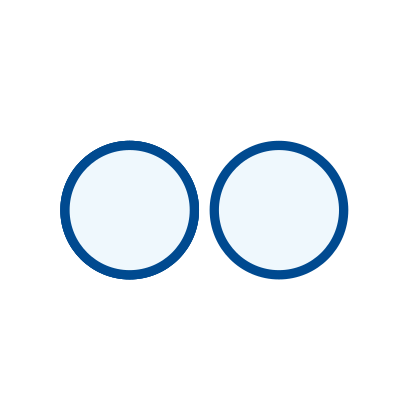
\includegraphics[height=\iconheight]{icons/normal.png}}
\newcommand{\hard}{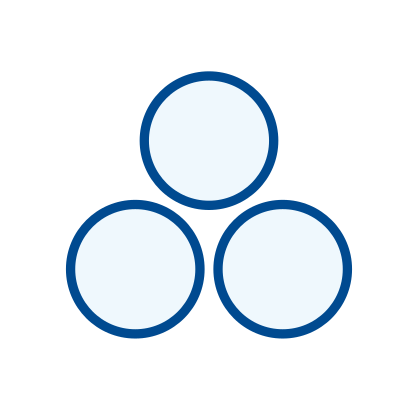
\includegraphics[height=\iconheight]{icons/hard.png}}
\newcommand{\hint}{
\includegraphics[height=\iconheight]{icons/hint.png}}
\newcommand{\solution}{
\includegraphics[height=\iconheight]{icons/answer.png}}
\newcommand{\ugent}{
\includegraphics[height=\iconheight]{icons/ugent.png}}
\newcommand{\youtube}{\,\,
\includegraphics[height=\iconheight]{icons/video.png}\,\,\,}


\newcommand{\sectionmarginoffset}{-1pt} % hack
\newcommand{\sectionyoutubeugent}[2]{\section[#1]{\noindent\marginnote[\sectionmarginoffset]{\href{https://youtu.be/#2}{\youtube}\,\ugent}#1}}
\newcommand{\sectionyoutube}[2]{\section[#1]{\noindent\marginnote[\sectionmarginoffset]{\href{https://youtu.be/#2}{\youtube}}#1}}
\newcommand{\sectionugent}[1]{\section[#1]{\noindent\marginnote[\sectionmarginoffset]{\ugent}#1}}

\begin{document}

%----------------------------------------------------------------------------------------
%	BOOK INFORMATION
%----------------------------------------------------------------------------------------

\titlehead{}
\title[Mathematics for Photonics]{Mathematics for Photonics}
\author[PB]{Peter Bienstman}
\date{\today}

%----------------------------------------------------------------------------------------

\KOMAoptions{twoside=semi}
%%\thispagestyle{empty}

%\oddsidemargin -.9in
\begin{figure}
\centering
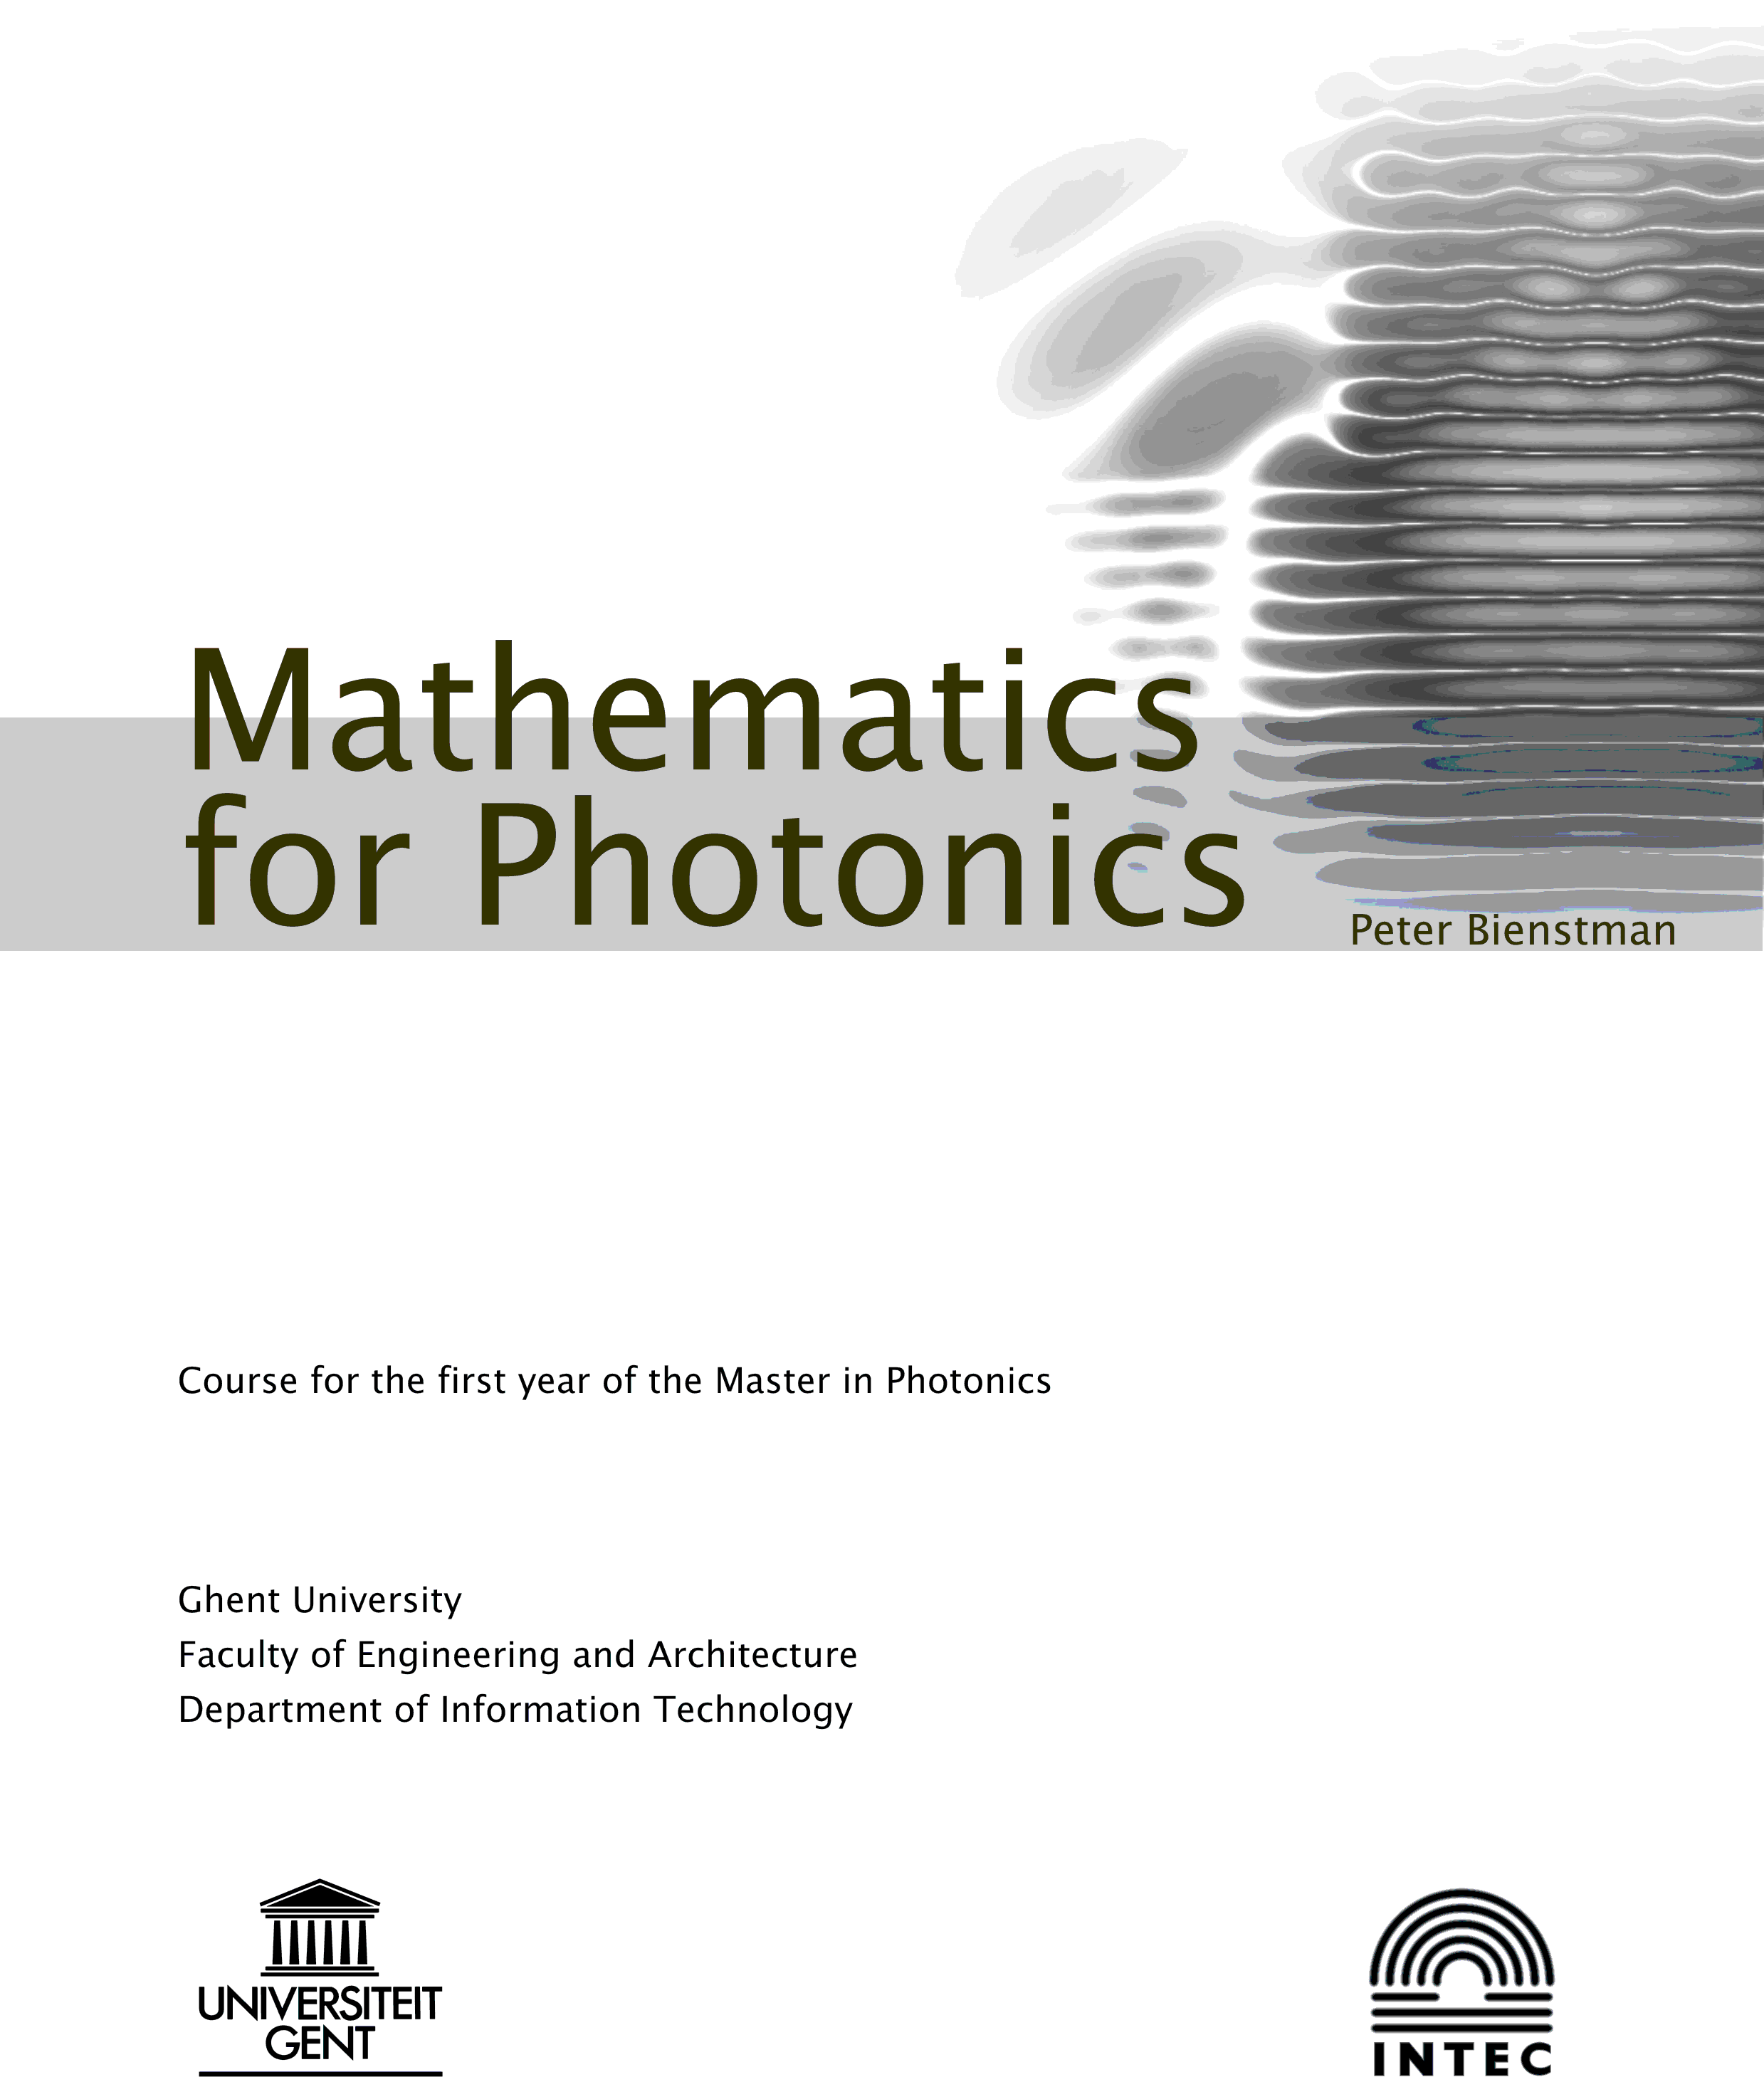
\includegraphics[width=\textwidth]{preamble/frontpage}
\end{figure}

%\mbox{}\\[3cm]

%\begin{center}
%{\Huge Mathematics for Photonics}\\[30mm]
%{\centering \large Peter Bienstman}\\[45mm]
%\end{center}

%{\noindent 1st year Master in Photonics course}\\[10mm]

%{\noindent Academic year 2004-2005} \\[10mm]


%{\noindent Ghent University}\\
%{Faculty of Applied Sciences}\\
%{Department of Information Technology}\\

%\thispagestyle{empty}


%\end{titlepage} %%%%%

%\thispagestyle{empty}

\cleardoublepage

%%% Local Variables:
%%% mode: latex
%%% TeX-master: "../main"
%%% End:

\KOMAoptions{twoside=false}

\frontmatter % Denotes the start of the pre-document content, uses roman numerals

\setcounter{page}{1}

%----------------------------------------------------------------------------------------
%	COPYRIGHT PAGE
%----------------------------------------------------------------------------------------

\makeatletter
\uppertitleback{\@titlehead} % Header

\lowertitleback{
	
	\textbf{Licence} \\
	\ccbyncsa \\
	This work is licenced under a Creative Commons 4.0 Attribution-NonCommercial-ShareAlike licence.
	
	%\medskip
	
	%\textbf{Publisher} \\
	%First printed in May 2019 by \@publishers
}
\makeatother

%----------------------------------------------------------------------------------------
%	DEDICATION
%----------------------------------------------------------------------------------------

%\dedication{
%	The harmony of the world is made manifest in Form and Number, and the heart and soul and all the poetry of Natural Philosophy are embodied in the concept of mathematical beauty.\\
%	\flushright -- D'Arcy Wentworth Thompson
%}

%----------------------------------------------------------------------------------------
%	OUTPUT TITLE PAGE AND PREVIOUS
%----------------------------------------------------------------------------------------

% Note that \maketitle outputs the pages before here

% If twoside=false, \uppertitleback and \lowertitleback are not printed
% To overcome this issue, we set twoside=semi just before printing the title pages, and set it back to false just after the title pages
\KOMAoptions{twoside=semi}
\maketitle
\KOMAoptions{twoside=false}

%----------------------------------------------------------------------------------------
%	PREFACE
%----------------------------------------------------------------------------------------


\chapter*{Preface}
\label{h:Preface}

The aim of this course is to expose students to various mathematical concepts often used in the field of photonics. Neither mathematical rigour nor extensive detail are envisaged, as the purpose of this course is to get students acquainted with a wide range of basic principles, which should allow them to independently refine their knowledge of mathematical topics that might emerge during their later career. As such, an important emphasis is placed on demonstrating the links of these mathematical concepts to concrete problems in the field of photonics.

The list of topics treated in this course also illustrates this focus on breath rather than depth:

The first four chapters deal with solving the wave equation in the case of time-harmonic optical signals, which gives rise to an equation in the complex plane. Chapter 1 therefore gives a brief introduction to complex calculus. Chapter 2 treats the solution of this equation for various special cases, for which we will need special functions and orthogonal polynomials. In order to solve this equation in the general case however, numerical techniques are required, so Chapter 3 will briefly discuss finite elements, finite differences and expansion in basis functions. Finally, Chapter 4 deals with the influence of periodicity and symmetry on the solutions of the complex wave equation.

After having treated time-harmonic systems, Chapter 5 will consider dynamical optical systems where the solutions can have a more general time dependence.

Finally, we wish to thank the people who provided feedback for this course and pointed out errors: Peter Vandersteegen, Kristof Vandoorne, Lieven Verslegers, Karel Van Acoleyen, Ziyue Zhang, Yancan Wu, Ruqi Shi, Martin Virte. We are also grateful to Wim Bogaerts for providing some of the figures for Chapter 4.\\[1cm]

\hspace{10cm} Peter Bienstman

\chapter{How to use this text}

\newcommand{\iconoffset}{\raisebox{-.25\height}} 

Research has shown that the best way to learn and master a subject, and especially one like mathematics, is through \textbf{active learning}: you have to grapple with the material yourself, trying to wrap your head around it and trying to understand how it fits together with concepts you already know. Also, you have to try and apply your knowledge creatively in new situations, as opposed to just passively absorbing how someone else has done this before. Listening to a lecture, however expertly given, or reading through an explanation, however clearly written down, actually does surprisingly little to form the brain connections that are required for you to truly master the material.

This text is constructed based on these observations. First of all, what in other textbooks would be a long theoretical explanation, is split up using \textbf{cues}:

\begin{cue}
\textbf{Cues} will give you a couple of hints, and based on these, you should take the next steps in the derivation yourself. That way, you will recall the material much better, and you will also be able to identify the gaps in your knowledge.
\end{cue}

We strongly encourage you to really take the time to actually work through these steps yourself. The temptation to skip ahead to the result, which is presented just below, is obviously great, given the attractiveness of the path of least resistance. However, doing so would deprive you of a valuable opportunity to process the material yourself, and would only lead to a superficial illusion of competence, and ultimately, a waste of time.

A second ingredient for active learning are the diverse \textbf{exercises}:

\begin{exunmarked}
\textbf{Exercises} are crucial to allow you to practice what you have learned in many different circumstances. The majority of your effort should be spent on them. Also here, actually put in the effort yourself, as opposed to wasting your time by just looking up the solution without an honest attempt to wrestle with the problem.
\end{exunmarked}

The exercises are (somewhat subjectively) ranked in three different levels:

\begin{itemize}
\item \iconoffset\trivial : trivial problems, just to get you used to the new concepts.
\item \iconoffset\normal : problems with 'normal' difficulty, that you should be able to tackle after some thought.
\item \iconoffset\hard : hard problems, for when you like more of a challenge.
\end{itemize}

For some of these hard problems, hints\iconoffset\hint are provided, which lower the difficulty from a hard problem to a regular one. Feel free to use these hints, at least after banging your head against the problem for a while.

Many exercises also include a solution \iconoffset\solution, so that you can check your answers.

In the ebook version of this text, you can click on the\iconoffset\hint or \iconoffset\solution icons to view hints or solutions. Clicking on the exercise number in the solution or hint chapter will take you back to the exercise itself.

There is also an amount of \textbf{video material} to support this text (still growing). Clicking the video icon \iconoffset\youtube will take you to the video of the corresponding exercise or theory part. Exercise solution videos are only there as a safety net, in case you get stuck or when you want to double check your intermediate steps. The main purpose of the theory videos is to provide people who prefer listening to a human over reading text, with an alternative way of being exposed to the material. In case you understand everything just by working with the text, there is absolutely no need to waste your time watching the videos, since they do not contain extra material or new insights (unless explicitly mentioned). On the other hand, if your preferred way of working is through the videos, we still recommend you to read this text, as being able to concentrate on a non-trivial amount of textual material is a useful skill to cultivate.

\textbf{Review questions} are also included and refer to the main basic concepts of the material. Reviewing these from time to time is a helpful way to solidify the most important points in your mind.

We also encourage you to create your \textbf{own summaries} or mind maps of the discussed concepts (preferably in handwriting), as a way to further actively engage with the material and to help you see the connections between different parts of this text.

Finally, since this is so crucial, let us once more repeat the only way to master the material:
\\

\fbox{\textbf{Do not skip to solutions or explanations before putting in some serious effort!}}


%%% Local Variables:
%%% mode: latex
%%% TeX-master: "../main"
%%% End:

\chapter{Practical aspects related to the course}

The \textbf{contact hours} of this course are a mix between a flipped classroom and a study group. To explain the rational behind this, let's first look at some drawbacks of other models:

A traditional theory lecture is a quite inefficient way of transferring knowledge. Some people quip that a lecture is a way to transfer information from the notes of the instructor to the notes of the student, without passing through the brains of either...

In a flipped classroom model, students are asked to study the material beforehand, and then use the time in class to ask questions or solve exercises. This works fine, unless you had an exceptionally busy week (let's face it, life happens!) and could not preread the lecture notes. In that case, you would be wasting your time in class.

Solving exercises all together in class is also not an optimal use of everybody's time. If you're quick and you've finished all the assigned exercises, you're wasting your time at that point. If you need a bit more time to work on a exercise (which is perfectly fine!), when the instructor brings the solution to the board, they deny you an important learning opportunity, when you would have been able to solve it completely by yourself if only you had had a few more minutes.

This means that the optimal way to work through the material, which is most respectful of everybody's time, is essentially self-paced, instead of following a rythm which is collectively imposed on the entire class. This self-pacing is facilitated through the existence of solutions, video clips, etc... (again, as a safety net to check your answers, not as a deceptive low-effort shortcut).

Therefore, in class, a combination of the following can happen:

\begin{itemize}
\item Anonymous multiple choice quizzes to help you assess your progress and to help the instructors identify problems.
\item Working in small groups through questions or exercises suggested by the instructor, if that's how you prefer to learn.
\item Working at your own pace through theory and exercises.   
\end{itemize}

An instructor is present to guide you and to answer any questions you might have.

A UGent icon \iconoffset\ugent\, indicates the minimum set of theory and exercises you should cover for this course. We do hope that you will go beyond that minimum, especially when it comes to the exercises.

To help you monitor your progress, the following table gives you a rough indication of what material you should have covered after each week:

\begin{center}
\begin{tabular}{ |c|c| } 
 \hline
  \textbf{Week} & \textbf{Material} \\
  \hline
 Week 1 & Section \ref{week1} \\ 
 Week 2 & Section \ref{week2} \\
 Week 3 & Section \ref{week3} \\
 Week 4 & Section \ref{week4} \\
 Week 5 & Section \ref{week5} \\
 Week 6 & Section \ref{week6} \\ 
 Week 7 & Section \ref{week7} \\
 Week 8 & Section \ref{week8} \\
 Week 9 & Section \ref{week9} \\
 Week 10 & Section \ref{week10}  \\
 Week 11 & Section \ref{week11} \\ 
 Week 12 & Section \ref{week12} \\
 \hline
\end{tabular}
\end{center}

Your final grade for this course is a combination of three factors:

To gently encourage you to put in sustained effort throughout the semester, as opposed to wasting your time by cramming just before the exam, we ask that every week you email us the written traces of your engagement with this course (solved cues, exercices, ...). Do not spend any time cleaning these up, your draft notes are perfectly fine, even if they are difficulty to read or messy, as we only consider whether or not you were active, and not the details of your notes. So, this is very different from homework. Email either a scanned version of your paper notes, or pictures of the pages you took with your phone using a tool like Microsoft Lens or Google Lens. You are allowed to skip two weeks, to accomodate for exceptional circumstances. \textbf{Weekly mailing your notes} counts for 5 points out of 20 for the final grade.

We also ask that you provide \textbf{improvements to the course text}, either in the form of corrections, clearer formulations of things you found confusing, new exercises, new theory topics, ... . This counts for 2 points. The best entries will be incorporated in the next version of these notes.

Finally, the remainder of your grade consists of the exam, which is an \textbf{oral open book exam}. The main goal of the exam is to check that you thoroughly internalised the concepts in the course and that you can apply them. In terms of exercises, you are expected to be able to do trivial\iconoffset\trivial exercises on the fly. For problems belonging to the normal \iconoffset\normal\, category, which are a bit more involved, we are only interested in your general strategy to tackle them, and not the detailed calculations. The point of the exam is NOT to check your ability to accurately perform calculations under stress, nor to see how creative you can be under time pressure. 

%%% Local Variables:
%%% mode: latex
%%% TeX-master: "../main"
%%% End:


%----------------------------------------------------------------------------------------
%	TABLE OF CONTENTS & LIST OF FIGURES/TABLES
%----------------------------------------------------------------------------------------

\begingroup % Local scope for the following commands

% Define the style for the TOC, LOF, and LOT
%\setstretch{1} % Uncomment to modify line spacing in the ToC
\hypersetup{linkcolor=headingblue} % Uncomment to set the colour of links in the ToC
\setlength{\textheight}{230\vscale} % Manually adjust the height of the ToC pages

% Turn on compatibility mode for the etoc package
\etocstandarddisplaystyle % "toc display" as if etoc was not loaded
\etocstandardlines % "toc lines as if etoc was not loaded

\tableofcontents % Output the table of contents

%\listoffigures % Output the list of figures

% Comment both of the following lines to have the LOF and the LOT on different pages
%\let\cleardoublepage\bigskip
%\let\clearpage\bigskip

%\listoftables % Output the list of tables

\endgroup

%----------------------------------------------------------------------------------------
%	MAIN BODY
%----------------------------------------------------------------------------------------

\mainmatter % Denotes the start of the main document content, resets page numbering and uses arabic numbers
\setchapterstyle{kao} % Choose the default chapter heading style

%\setcounter{chapter}{-1}
\setchapterpreamble[u]{\margintoc}
\chapter{The Helmholtz equation}
\label{h:helmholz}

In this introductory chapter, we will review the Helmholtz equation, as it is fundamental in photonics, and will be used in many of the subsequent chapters.

\sectionyoutubeugent{Maxwell's equations in the frequency domain}{Rx6ptGNSuKA}

\begin{marginfigure}[+0.0cm]
  % credits: Wikipedia
  % url: https://en.wikipedia.org/wiki/James_Clerk_Maxwell#/media/File:James_Clerk_Maxwell.png
  \includegraphics{helmholtz/figures/james_clerk_maxwell}
  \caption{James Clerk Maxwell (1831-1879)}
\end{marginfigure}

To start with, let's recall Maxwell's curl equations in the time domain. In the absence of current sources, they are given by

\begin{equation}
\nabla \times {\mathbf E} ({\mathbf r},t) = - \mu({\mathbf r)} \frac{\partial {\mathbf H} ({\mathbf r} ,t)}{\partial t} \label{eq-rot-E}
\end{equation}
\begin{equation}
\nabla \times {\mathbf H} ({\mathbf r},t) = \varepsilon({\mathbf r}) \frac{\partial {\mathbf E}({\mathbf r},t)}{\partial t} \label{eq-rot-H}
\end{equation}

For the common case of linear isotropic media, the dielectric permittivity $\varepsilon$ and the magnetic permeability $\mu$ are scalars, which can however be a function of the spatial coordinate ${\mathbf r}$.

In the next chapters, we will restrict ourselves to the important case where all the fields have a harmonic time dependence with a fixed frequency $\omega$, e.g. for the $x$--component of the electric field:

\begin{equation}
E_x({\mathbf r},t) = E_{x,0}({\mathbf r}) \cos \left( \omega t + \phi_{E_x} ({\mathbf r})
\right) \label{eq-phasor}
\end{equation}

Similar expressions can be written for the other field components and for the magnetic field. It is convenient to introduce a complex number $\tilde{E}_x$ called a \emph{phasor}, that is defined as

\begin{equation}
\tilde{E}_x(\mathbf{r})=E_{x,0}({\mathbf r}) e^{j \phi_{E_x}({\mathbf r})} \label{eq:phasor}
\end{equation}

\begin{cue}
Given such a complex-valued phasor, how can we recover the real-valued electric field?
\end{cue}

\noindent\marginnote{Note that some people use a different convention, which results in $e^{-j \omega t}$. This can give rise to some surprising sign changes in formulas, so be aware of this!}The relation between the phasor and the electric field is given by

\begin{equation}
E_x({\mathbf r},t) = \Re \left(\tilde{E}_x({\mathbf r}) e^{j \omega t}\right)
\end{equation}

\begin{cue}
What is the phasor corresponding to $\partial E_x({\mathbf r},t) / \partial t$ ?
\end{cue}

By taking the time derivative of Eq.~\ref{eq-phasor}, it is easy to show that 

\begin{equation}
\frac{\partial E_x({\mathbf r},t)}{\partial t} = \Re \left(j \omega \tilde{E}_x({\mathbf r}) e^{j \omega t}\right)
\end{equation}

Therefore, the phasor corresponding to $\partial E_x({\mathbf r},t) / \partial t$ is given by $j \omega \tilde{E}_x({\mathbf r})$.

In what follows, we will omit the tilde and implicitly assume that we are always dealing with phasors. We can also collect the phasors for all field components in complex vectors ${\mathbf E}$ and ${\mathbf H}$. 

\begin{cue}
Write Eq.~\ref{eq-rot-E} and \ref{eq-rot-H} using phasor notation.
\end{cue}

Using phasor notation, Eq.~\ref{eq-rot-E} and \ref{eq-rot-H} become

\begin{equation}
\nabla \times {\mathbf E}({\mathbf r}) = - j \omega \mu({\mathbf r}) {\mathbf H}({\mathbf r})
\label{eq-rot-E-phas}
\end{equation}
\begin{equation}   
\nabla \times {\mathbf H}({\mathbf r}) = j \omega \varepsilon({\mathbf r}) {\mathbf E}({\mathbf r}) \label{eq-rot-H-phas}
\end{equation}

These are Maxwell's equations expressed in the frequency domain.

\begin{exer}
  % difficulty: trivial
  % ugent
  What phasor corresponds to time integration of $\tilde{E}_x$?
\end{exer}

\begin{exer}
  % difficulty: trivial
 How do you need to change Eq.~\ref{eq-phasor}, so that the time dependence of a phasor corresponds to $e^{-j \omega t}$? 
\end{exer}

\sectionugent{The Helmholtz equation}

\begin{cue}
Take the curl of Eq.~\ref{eq-rot-E-phas} and use Eq.~\ref{eq-rot-H-phas}.
\end{cue}

By taking the curl of Eq.~\ref{eq-rot-E-phas} and plugging Eq.~\ref{eq-rot-H-phas} in the result, we get

\begin{equation}
  \nabla \times \nabla \times {\mathbf E}({\mathbf r}) = \omega^2 \varepsilon({\mathbf r}) \mu({\mathbf r}) {\mathbf E}({\mathbf r})
  \label{eq-helm-1}
\end{equation}

From vector calculus we know that

\begin{equation}
\nabla \times \nabla \times {\mathbf E}({\mathbf r}) = \nabla (\nabla \cdot {\mathbf E}({\mathbf r})) - \nabla^2 {\mathbf E}({\mathbf r})
\end{equation}

\begin{cue}
Use this to simplify Eq. \ref{eq-helm-1} in a uniform medium without charge $\rho$. 
\end{cue}

Let's for the moment consider a uniform medium without charge $\rho$. In that case, Maxwell's divergence laws tell us that $\nabla \cdot {\mathbf E}({\mathbf r})=0$, leading to

\begin{equation}
\nabla^2 {\mathbf E}({\mathbf r}) + k^2 {\mathbf E}({\mathbf r}) = 0 \label{eq-helmholtz}
\end{equation}

where we have introduced the wave vector $k=\omega \sqrt{\varepsilon \mu}$.

Eq.~\ref{eq-helmholtz} is called the (vectorial) Helmholtz equation. Note that the same equation can also be derived for the magnetic field ${\mathbf H}$. In Cartesian coordinates, each of the vectorial components of ${\mathbf E}$ and ${\mathbf H}$ satisfy a scalar Helmholtz equation:

\begin{marginfigure}[-0.0cm]
  % credits: Wikipedia
  % url: https://en.wikipedia.org/wiki/Hermann_von_Helmholtz#/media/File:Hermann_von_Helmholtz.jpg
  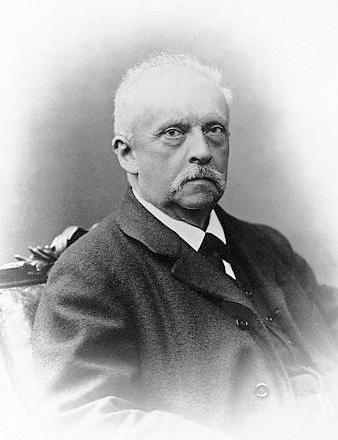
\includegraphics{helmholtz/figures/Hermann_von_Helmholtz}
  \caption{Hermann von Helmholtz (1821-1894)}
\end{marginfigure}

\begin{equation}
\nabla^2 \psi({\mathbf r}) + k^2 \psi({\mathbf r}) = 0 \label{eq-helmholtz-1}
\end{equation}

Now, if we are studying a system which has a piecewise constant refractive index, Eq.~\ref{eq-helmholtz-1} will be valid in each of the uniform subregions. So formally we can write for the scalar Helmholtz equation in a medium with discrete index jumps:

\begin{equation}
\fbox{$\displaystyle \nabla^2 \psi({\mathbf r}) + k_0^2 n^2({\mathbf r}) \psi({\mathbf r}) = 0
\label{eq-helmholtz-3}$}
\end{equation}

Here, $k_0=\omega \sqrt{\varepsilon_0 \mu_0}$ is the wave vector in vacuum, and the refractive index $n$ is defined by $n=\sqrt{\varepsilon \mu} \sqrt{\varepsilon_0 \mu_0}$.

Eq.~\ref{eq-helmholtz-3} is strictly speaking only valid \emph{inside} each uniform subregion. At the interface between different media we still have to deal with the appropriate continuity conditions for the fields.

Since $\psi$ is a complex number, it seems worthwhile to study the calculus of functions of a complex variable. We will see that this has a number of direct applications in photonics, e.g. the Kramers--Kronig dispersion relations, and the use of conformal transformations to study waveguide bends.

\begin{exer}
    % difficulty: trivial
Solve the Helmholtz equation in a single uniform medium.
\end{exer}

\begin{exer}
    % difficulty: trivial
What does the Helmholz equation look like in case we use the time convention  $e^{-j \omega t}$? 
\end{exer}

\begin{exer}
      % difficulty: hard
The Helmholtz equation we derived here is only valid for uniform media. Exactly which step of the derivation breaks down in non-uniform media?
\end{exer}

\section*{Review questions}

\begin{itemize}
\item What is a phasor?
\item Write down Maxwell's curl equations in the frequency domain.
\item Write down the Helmholtz equation.
\end{itemize}



%%% Local Variables:
%%% mode: latex
%%% TeX-master: "../main"
%%% End:

%\chapter{Complex calculus}
\label{h:complex}

\begin{quote}
The shortest path between two truths in the real domain passes through the complex domain.

--- Jacques Hadamard
\end{quote}

\begin{quote}
The imaginary number is a fine and wonderful recourse of the divine spirit, almost an amphibian between being and not being.

--- Gottfried Wilhelm Leibniz
\end{quote}

\begin{quote}
  Life is complex: it has both real and imaginary components.
  
--- Rich Rosen
\end{quote}

\chaptertoc

In this chapter, we will discuss the basic principles of complex analysis and its applications.

We will define functions of a complex variable and show how to differentiate and integrate them. In order to facilitate the calculation of integrals, residue calculus is introduced. This will give us a powerful tool to also calculate some real-valued integrals in a much more straightforward way. Finally, we discuss conformal transformations as a way to map problems to equivalent ones having an 'easier' geometry. 

We will also study a number of direct applications of complex analysis, e.g. the Kramers--Kronig dispersion relations, and the use of conformal transformations to model waveguide bends.



\pagebreak


\sectionugent{Functions of a complex variable}

A function of a complex variable is simply defined as

\begin{equation}
f(z) \stackrel{def}{=} f(x + j y) \stackrel{def}{=}  u(x,y) + j v(x,y)
\end{equation}

Here, $u$ and $v$ are two real--valued functions of $x$ and $y$. Unsurprisingly, we call $u$ the real part of $f$ and $v$ the imaginary part of $f$.

\begin{cue}
Take
$$u = x^2 - y^2$$
$$v = 2 x y$$
What is $f(z)$?
\end{cue}

In this case,

$$f(z) = u + j v = x^2 - y^2 +2j x y = (x + jy)^2$$

So, formally we can say that $u$ and $v$ define the function $f(z) = z^2$

\begin{cue}
Given
$$f(z) = z z^* $$
such that
$$f(z) = (x + jy)(x - jy) = x^2 + y^2$$

What are the corresponding $u$ and $v$?
\end{cue}

The real and imaginary parts are:

$$u = x^2 + y^2$$
$$v = 0$$


\pagebreak


\sectionugent{Derivatives of complex functions}

Let us now differentiate complex functions. In analogy with real--valued functions, we would like to define the complex derivative as

\begin{equation}
f' (z)=\frac{df}{dz} \stackrel{def}{=} \lim_{\Delta z \to 0} \frac{f(z+\Delta z) - f(z)}{z+\Delta z - z} \label{eq-deriv}
\end{equation} 

\begin{cue}
Use this definition to find the derivative of $f(z)=z^2$.
\end{cue}

To calculate the derivative of  $f(z)=z^2$, we find that

$$f'(z)=\lim_{\Delta z \to 0} \frac{(z+\Delta z)^2 - z^2}{\Delta z} = \lim_{\Delta z \to 0} \frac{2 z \Delta z + (\Delta z)^2}{\Delta z}=2z $$

This gives the same result as in the real-valued case.

At this point, you might wonder what all the fuzz is about, as complex analysis seems to boil down to simply replacing $x$ by $z$. However, there's more going on than meets the eye.

\begin{cue}
Try to find the derivative of $f(z)=|z|^2$.
\end{cue}

In this case, we get

$$f'(z)=\lim_{\Delta z \to 0} \frac{|z+\Delta z|^2 - |z|^2}{\Delta z} $$

The numerator is obviously real-valued, but the denominator is in general complex, so that the result of this operation would depend on the direction of approach encoded in $\Delta z$.

This is obviously undesirable. Now, we can ask ourself the question, what are the conditions under which the derivative Eq.~\ref{eq-deriv} of a complex function is independent of the direction of approach?

\begin{marginfigure}[-2cm]
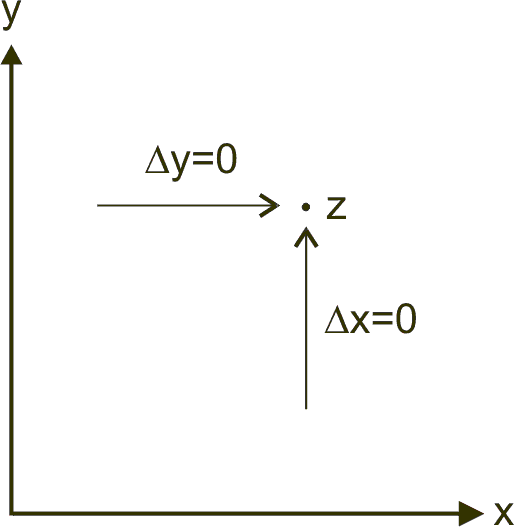
\includegraphics[width=4cm]{complex/figures/approach_z}
\caption{Different approaches to $z$ in the complex plane.}
\label{fig-approach-z}
\end{marginfigure}

Let's have a look at the necessary conditions first. If the direction of approach does not matter at all, than we should certainly get the same result if we pick two special directions (see Fig.~\ref{fig-approach-z}).

\begin{cue}
 By splitting both $f$ and $z$ into their real and imaginary components, take the limit of $\Delta f / \Delta z$ along the horizontal direction.
\end{cue}

Along the horizontal direction, $\Delta y = 0$, so taking the limit $\Delta x \to 0$, we get

\begin{align}
\lim_{\Delta z \to 0} \frac{\Delta f}{\Delta z}
& = \lim_{\Delta z \to 0} \frac{\Delta u + j \Delta v}{\Delta x + j \Delta y}
\nonumber \\
& = \lim_{\Delta x \to 0} \frac{\Delta u}{\Delta x} + j \frac{\Delta v}{\Delta
x} \nonumber \\
& = \frac{\partial u}{\partial x} + j \frac{\partial v}{\partial
x}\label{eq-deriv-dx}
\end{align} 

\begin{cue}
Do the same for an approach along the vertical direction.
\end{cue}

Along the vertical direction, $\Delta x = 0$ and we should take the limit $\Delta y \to 0$:

\begin{align}
\lim_{\Delta z \to 0} \frac{\Delta f}{\Delta z}
& = \lim_{\Delta z \to 0} \frac{\Delta u + j \Delta v}{\Delta x + j \Delta y}
\nonumber \\
& = \lim_{\Delta y \to 0} -j\frac{\Delta u}{\Delta y} +  \frac{\Delta v}{\Delta
y} \nonumber \\
& = -j\frac{\partial u}{\partial y} +  \frac{\partial v}{\partial
y}\label{eq-deriv-dy}
\end{align}

\begin{cue}
Now derive a necessary condition for the complex derivative to be independent of the direction of approach.
\end{cue}

A necessary condition for the complex derivative to be independent of the direction of approach, can be derived from equating the real and imaginary parts of Eq.~\ref{eq-deriv-dx} and \ref{eq-deriv-dy}:

\begin{equation}
\fbox{$\displaystyle
\frac{\partial u}{\partial x} = \frac{\partial v}{\partial y}, \hspace{.5cm}
\frac{\partial v}{\partial x} = -\frac{\partial u}{\partial y}
\label{eq-Cauchy-Riemann}
$}
\end{equation} 

\begin{marginfigure}[-4.0cm]
  % credits: Wikipedia
  % url: https://en.wikipedia.org/wiki/Bernhard_Riemann#/media/File:Georg_Friedrich_Bernhard_Riemann.jpeg
  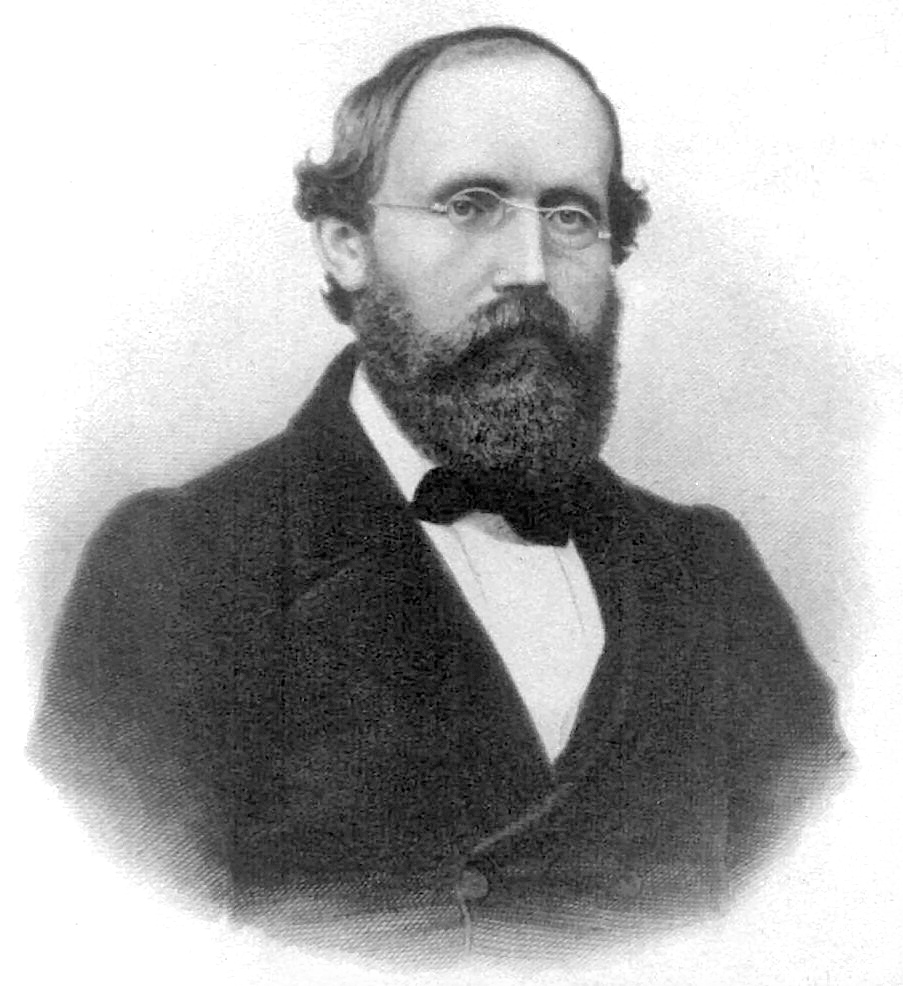
\includegraphics{complex/figures/b_riemann}
  \caption{Bernhard Riemann (1826-1866)}
\end{marginfigure}

These are called the \emph{Cauchy--Riemann conditions}. A complex function that satisfies these conditions is called \emph{analytic} (or holomorphic). Important to note is that for a function to be analytic, it necessarily has to be continuous and should not contain any singularities, otherwise the derivative would certainly be undefined.

We will now show that the Cauchy--Riemann conditions are not only necessary, they are also sufficient (assuming all partial derivatives are continuous).

We can write the total differential

\begin{equation}
d f = \left( \frac{\partial u}{\partial x}+j\frac{\partial v}{\partial x}\right) d x+\left(\frac{\partial u}{\partial y}+j\frac{\partial v}{\partial y}\right) d y
\end{equation} 

such that

\begin{equation}
\frac{d f}{d z} = \frac{\left(\frac{\partial u}{\partial x}+j\frac{\partial v}{\partial x}\right) d x+\left(\frac{\partial u}{\partial y}+j\frac{\partial v}{\partial y}\right) d y}{d x + j d y}
\end{equation} 

or

\begin{equation}
\frac{d f}{d z} = \frac{\left(\frac{\partial u}{\partial x}+j\frac{\partial v}{\partial x}\right) +\left(\frac{\partial u}{\partial y}+j\frac{\partial v}{\partial y}\right) \frac{d y}{d x}}{1 + j \frac{d y}{d x}} \label{eq-cr-suf}
\end{equation} 

\begin{cue}
Where in Eq.~\ref{eq-cr-suf} is the direction of approach encoded? Get rid of that term by applying the Cauchy-Riemann conditions.
\end{cue}

We now need to prove that this expression is independent on $d y / d x$ in order for the complex derivatives to be independent of the direction of approach. Indeed, each direction of approach will have its own value of $d y / d x$ .

Applying the Cauchy--Riemann conditions to the $y$--derivatives, we obtain

\begin{equation}
\frac{\partial u}{\partial y}+j\frac{\partial v}{\partial y} = -\frac{\partial v}{\partial x}+j\frac{\partial u}{\partial x}
\end{equation}

Substituting this into Eq.\ref{eq-cr-suf}, we get that the $d y / d x$ dependence cancels out to give

\begin{equation}
\fbox{$\displaystyle
\frac{d f}{d z} = \frac{\partial u}{\partial x}+j\frac{\partial v}{\partial x}
$}
\end{equation} 

This equation also shows that only derivatives with respect to $x$ are needed to calculate the complex derivative.

\pagebreak

\begin{exer}
% difficulty: trivial
% ugent
% youtube: l81NZVwQmW0
Are the following functions analytic? If so, calculate their derivative.
$$\begin{array}{lcll}a) & f(z)=z^2 \\b) & f(z)=z z^* \\c) & f(z)= \Re(z)=x \end{array}$$

What rule-of-thumb can you derive from these results?

\begin{sol}
Analytical and $f'(z)=2z$ / non-analytical / non-analytical. Real-valued functions where you replace $x$ by $z$ are typically analytical. Functions where you make explicit reference to the real and imaginary components of a complex number or to its complex conjugate are not.
\end{sol}
  
\end{exer}

\begin{exer}
  % difficulty: trivial
  % youtube: 8wbS4_Ztd3A
\label{ex-harmonic}
$u$ and $v$ are the real and imaginary parts, respectively, of an analytic function $f(z)$. Show that $u$ and $v$ are \emph{harmonic} functions, i.e. they satisfy Laplace's equation
$$\nabla^2 u = \nabla^2 v = 0$$
\end{exer}

\begin{exer}
  % difficulty: trivial
  % youtube: MZS3Z9o_Bs0
$u$ and $v$ are the real and imaginary parts, respectively, of an analytic function $f(z)$. Show that $|f'(z)|^2$ is equal to the Jacobian determinant
$$\frac{\partial (u,v)}{\partial (x,y)} =  \begin{vmatrix} \partial u / \partial x & \partial u / \partial y \\ \partial v / \partial x & \partial v / \partial y \end{vmatrix}$$
\end{exer}


\pagebreak


\sectionugent{Integrals of complex functions}

With differentiation under control, it is time to study integrals of complex functions. The integral of a complex function along a specified path ${C}$ between $z_0$ and $z_1$ (see Fig.~\ref{fig-integral}) is defined by

\begin{marginfigure}[]
\centering
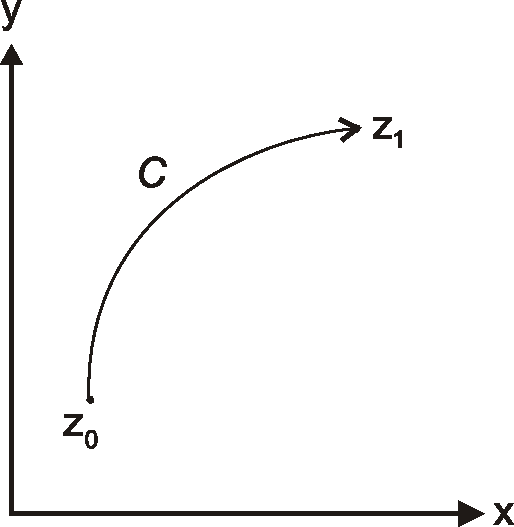
\includegraphics{complex/figures/integral}
\caption{A complex line integral.}
\label{fig-integral}
\end{marginfigure}

\begin{align}
\int_{C}f(z)dz = & \int_{C}\left(u(x,y)+jv(x,y)\right)(dx+jdy)
\nonumber \\
  = & \int_{C}\left[u(x,y)dx-v(x,y)dy\right] + \nonumber\\
  & j\int_{C}\left[v(x,y)dx+u(x,y)dy\right] \label{eq-complex-int}
\end{align} 

So, the integral of a complex function has been expressed in terms of well-known real line integrals, which are calculated in the normal way by parametrisation of the curve. (Note that in Eq.~\ref{eq-complex-int} $dx$ and $dy$ are not independent, but related by the choice of the integration path.)

Let's calculate the contour integral $\oint_{C}z^ndz$ where the contour ${C}$ is a counterclockwise circular path of radius $r$ around the origin $z=0$. Note that we do not necessarily need to split up the integral into its real and imaginary components, but that we can directly parametrise the complex path if we want.

\begin{cue}
Parametrise the curve in polar coordinates using $z=r\exp(j\theta)$ for $\theta=0\to 2 \pi$ and calculate the integral. 
\end{cue}

Expressing the unit cirle as $z=r\exp(j\theta)$ for $\theta=0\to 2 \pi$, we get

$$\oint_{C} z^n dz = \int_0^{2\pi} \left(r^n e^{jn\theta}\right) \left(jr e^{j \theta}d \theta\right)=j r^{n+1} \int_0^{2\pi} e^{j(n+1)\theta} d \theta $$

For $n \neq -1$ this is equal to

$$ \frac{r^{n+1}}{n+1}\left[e^{j(n+1)\theta}\right]_0^{2\pi}=0 $$

because of the periodicity of the exponential. For $n=-1$, we obtain 

$$ \oint_{C} \frac{dz}{z} = j \int_0^{2\pi} d \theta = 2 \pi j $$

which is independent of $r$.

Note that the results of this seemingly trivial integral will prove to have deep consequences later.

\begin{exer}
  % difficulty: trivial
  % youtube: i7F2OP3yENM
Revisit the calculation of  $\oint_{C}z^ndz$, but this time use the parametrisation  $z=r\exp(j\theta^2)$. 
\end{exer}


\pagebreak


\sectionugent{Cauchy's integral theorem}

\begin{marginfigure}[+0.3cm]
  % credits: Wikipedia
  % url: https://en.wikipedia.org/wiki/Augustin-Louis_Cauchy
  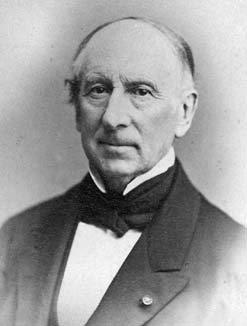
\includegraphics{complex/figures/cauchy}
  \caption{Augustin-Louis Cauchy (1789-1857)}
\end{marginfigure}

One of the major theorems in complex calculus is Cauchy's integral theorem. It states that 

\begin{equation}
\fbox{$\displaystyle
\oint_{{C}} f(z) dz = 0 \label{eq-cauchy-1}
$}
\end{equation}

Important to note is that Eq.~\ref{eq-cauchy-1} only holds if $f(z)$ is analytic for all the points enclosed by the contour ${C}$, as well as for the points on the contour itself. The symbol $\oint$ is used to emphasise that the path is closed.

\begin{cue}
To prove Eq.~\ref{eq-cauchy-1}, first apply the definition of the complex contour integral given in Eq.~\ref{eq-complex-int}.
\end{cue}

This gives

\begin{align}
\oint_{C}f(z)dz = & \oint_{C}\left(u(x,y)+jv(x,y)\right)(dx+jdy)
\nonumber \\
  = & \oint_{C}\left[u(x,y)dx-v(x,y)dy\right] + \nonumber \\
  & j \oint_{C}\left[v(x,y)dx+u(x,y)dy\right]  \label{eq-cauchy-proof}
\end{align}

\begin{marginfigure}[-0.0cm]
  % credits: Wikipedia
  % url: https://en.wikipedia.org/wiki/Sir_George_Stokes,_1st_Baronet#/media/File:Ggstokes.jpg
  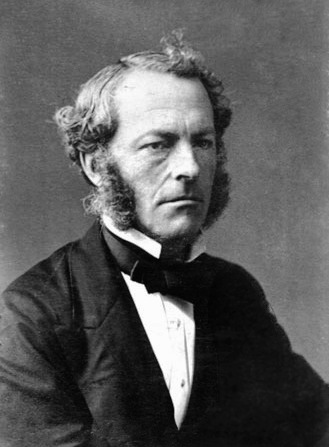
\includegraphics{complex/figures/stokes}
  \caption{George Stokes (1819-1903)}
\end{marginfigure}

In order to be able to use the Cauchy-Riemann conditions, we somehow need to bring partial derivatives into this formula. For this, we will use Stokes's theorem:

\begin{equation}
\oint_{{{C}}} {\mathbf A} \cdot d {\mathbf l} = \iint_S \nabla \times {\mathbf A} \cdot d {\mathbf S}
\end{equation}

\begin{cue}
Convert Stokes's theorem to our two-dimensional case.
\end{cue}

In two dimensions (i.e. $A_z=0$ and the contour contained in the $(x,y)$--plane), Stokes becomes:

\begin{equation}
\oint_{{C}} \left(A_x dx + A_y dy\right) = \iint_S \left(\frac{\partial
A_y}{\partial x} - \frac{\partial A_x}{\partial y} \right)dx dy
\end{equation} 

\pagebreak

\begin{cue}
Figure out which values of $A_x$ and $A_y$ to use, so that we can apply Cauchy--Riemann to the first term in Eq.~\ref{eq-cauchy-proof}.
\end{cue}

For the first term in Eq.~\ref{eq-cauchy-proof}, we choose $A_x=u$ and $A_y=-v$ such that

\begin{align}
\oint_{C}\left[u(x,y)dx-v(x,y)dy\right] =& \oint_{{C}} \left(A_x dx + A_y dy\right) \nonumber \\
=& \iint_S \left(\frac{\partial A_y}{\partial x} - \frac{\partial A_x}{\partial y} \right)dx dy \nonumber \\ =& -\iint_S \left(\frac{\partial v}{\partial x} + \frac{\partial u}{\partial y} \right)dx dy 
\end{align} 

Because of the Cauchy--Riemann conditions Eq.~\ref{eq-Cauchy-Riemann}, this
vanishes.

\begin{cue}
Which values of $A_x$ and $A_y$ should we use for the second term in Eq.~\ref{eq-cauchy-proof}?
\end{cue}

A similar conclusion can be drawn for the second term in Eq.~\ref{eq-cauchy-proof} by setting $A_x=v$ and $A_y=u$, which proves that the entire integral in Eq.~\ref{eq-cauchy-1} vanishes.

\begin{exer}
  % difficulty: trivial
  % youtube: _u3lqk3sxyQ
Prove that for an analytic function $f(z)$ the line integral 
$$\int_{z_0}^{z_1}f(z)dz$$
is independent on the exact path between $z_0$ and $z_1$.
\end{exer}


\pagebreak


\sectionugent{Cauchy's integral formula}
\label{week1}

The second major theorem in complex calculus is Cauchy's integral \emph{formula} (as opposed to Cauchy's integral \emph{theorem} from the previous section). Cauchy integral formula states that for an analytic function $f(z)$

\begin{equation}
\fbox{$\displaystyle
\frac{1}{2 \pi j}\oint_{{C}} \frac{f(z)} {z-z_0} dz = f(z_0)
\label{eq-cauchy-2}
$}
\end{equation}

Important here is that $z_0$ is a point enclosed by the contour ${C}$.

\begin{cue}
What would happen to Eq.~\ref{eq-cauchy-2} if  $z_0$ were outside of the contour?  
\end{cue}

If $z_0$ were outside of the contour, then the integrand of Eq.~\ref{eq-cauchy-2} would be analytic in the entire region enclosed by the contour. In that case, Cauchy's theorem applies and the integral vanishes.

\begin{marginfigure}[-1cm]
\centering
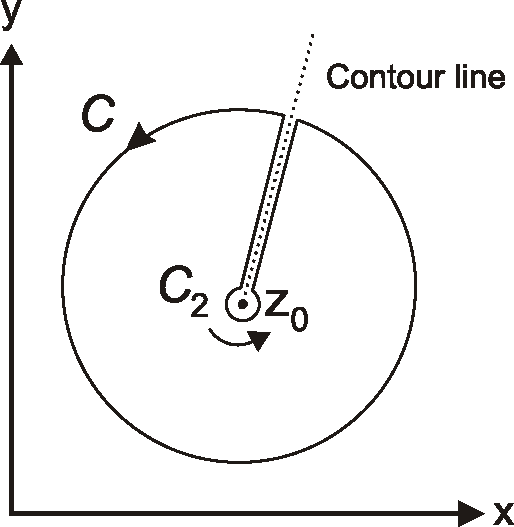
\includegraphics[width=5cm]{complex/figures/cauchy_II}
\caption{Contour to prove Cauchy's formula.}
\label{fig-cauchy-II}
\end{marginfigure}

To prove Eq.~\ref{eq-cauchy-2}, we note that although the function $f(z)$ is analytic, $f(z)/(z-z_0)$ is not, because is has a singularity at $z=z_0$. However, if we deform ${C}$ to exclude the singularity as in Fig.~\ref{fig-cauchy-II}, we end up with a contour where Cauchy's theorem does apply.

\begin{cue}
Apply Cauchy's theorem to this extended contour, splitting up the contributions from its different parts. What happens to the contributions of the straight lines?
\end{cue}

The result is

\begin{equation}
\oint_{{C}} \frac{f(z)} {z-z_0} dz -\oint_{{C}_2} \frac{f(z)}
{z-z_0} dz=0
\end{equation} 

Here, ${C}$ is the original outer contour and ${C}_2$ is the circle surrounding the point $z_0$ traversed in a counterclockwise direction (hence the minus sign). The two sections of the path along the contour line cancel because $f(z)$ is continuous (a side effect of it being analytic).

\begin{cue}
Parametrise ${C}_2$ and calculate its contribution to the integral. Then, take the limit $ r \to 0 $ to prove Cauchy's formula.   
\end{cue}

To calculate the integral along ${C}_2$, we use the parametrisation $z=z_0 + r e^{j\theta}$:

\begin{equation}
\oint_{{C}_2} \frac{f(z)} {z-z_0} dz = \oint_{{C}_2} \frac{f(z_0
+ r e^{j\theta})} {r e^{j\theta}} \left(rje^{j \theta} d \theta\right)
\end{equation}

In the limit $ r \to 0 $ this becomes

\begin{align}
\oint_{{C}_2} \frac{f(z)} {z-z_0} dz = & \, j f(z_0) \oint_{{C}_2} d \theta \nonumber \\
 = & \, 2 \pi j f(z_0)
\end{align}
 
which proves Cauchy's integral formula.

Note that this formula is quite remarkable. It means that as soon as the values of an analytic function are specified on a contour, we immediately know the function values at all the interior points.

\begin{exer}
% difficulty: trivial
% ugent
% youtube: F8DqIP6fnpw
Use Cauchy's formula to calculate 
$$\oint_{{C}}  \frac {e^z} {z+1} dz$$
Here ${C}$ is a circle of radius 4 centered at the origin.
\begin{sol}
$$\frac{2 \pi j}{e}$$
\end{sol}
\end{exer}

\begin{exer}
  % difficulty: normal
  % youtube: G4Fm4Vgk0VU
Use Cauchy's formula to calculate 
$$\oint_{{C}}  \frac {e^{az}} {z} dz$$
Here ${C}$ is the unit circle and $a$ is a real-valued constant. Then, write this integral in terms of $\theta$ and show
$$ \int_0^\pi e ^{a \cos \theta} \cos (a \sin \theta) d\theta = \pi $$
\begin{sol}
$$2 \pi j$$
\end{sol}
\end{exer}

\begin{exer}
% difficulty: hard
% ugent
% youtube: YtdU-XXWwnk
\label{ex-cauchy-diff}
Prove the following identity:

$$f'(z_0)=\frac{1}{2 \pi j} \oint_{{C}} \frac{f(z)} {(z-z_0)^2} dz$$

This expression can be used to (numerically) calculate the derivative of an analytic function.
\begin{hnt}
Apply Cauchy's formula to each of the terms of $$\frac{f(z_0+\Delta z_0) - f(z_0)}{\Delta z_0}$$ Then take the limit ${\Delta z_0} \to 0$.
\end{hnt}
\end{exer}

\begin{exer}
  % difficulty: hard
  % youtube: tyNs5agWKZw
Show that

  $$f^{(n)}(z_0)=\frac{n!}{2 \pi j} \oint_{{C}} \frac{f(z)} {(z-z_0)^{n+1}} dz$$
  
This also means that if a function is analytic, then the derivatives of any order automatically exist.
\begin{hnt}
Use induction and repeat the technique used in Ex. \ref{ex-cauchy-diff}.
\end{hnt}  
\end{exer}


\pagebreak


\sectionugent{Laurent series}


\begin{marginfigure}
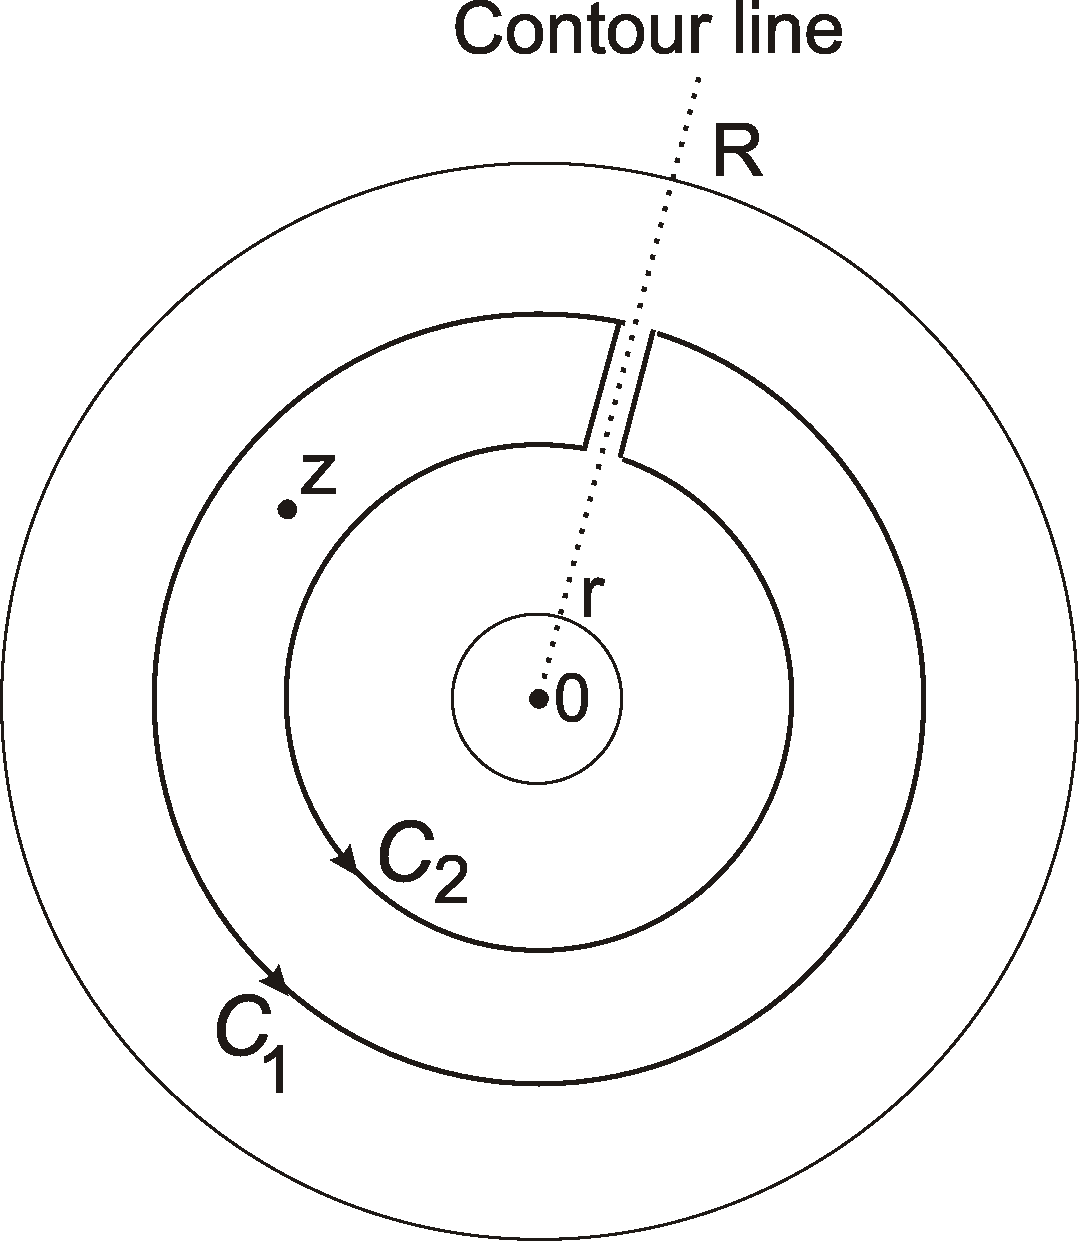
\includegraphics{complex/figures/laurent}
\caption{Contour to derive Laurent series.}
\label{fig-laurent}
\end{marginfigure}

Let's try to come up with a series expansion for complex functions. Here, special care has to be taken with respect to the convergence area. Consider e.g. a function that is analytic in some annular region around the origin of inner radius $r$ and outer radius $R$.

\begin{cue}
Would a circular contour work in this situation, if we want to apply Cauchy's formula?
\end{cue}

A simple circular contour would enclose the inner region where the function is not analytic, so we need to construct a more complicated contour that only encloses points where the function is analytic (Fig.~\ref{fig-laurent})

\begin{cue}
  Apply Cauchy's formula, splitting up the contour into its different parts.
\end{cue}

Cauchy's formula gives us

\begin{equation}
f(z)=\frac{1}{2 \pi j }\oint_{{C}_1} \frac{f(z')} {z'-z} dz' -\frac{1}{2
\pi j }\oint_{{C}_2} \frac{f(z')} {z'-z} dz' \label{laurent_0}
\end{equation} 

Here, $z$ is a fixed point on the inside of the contour, while $z'$ is the integration variable running along the contour. The two line segments cancel once again.

Our aim is to transform this formula into a series expansion. One can prove that the following straightforward generalisation of the well--known geometric series expansion holds:

\begin{equation}
\frac{1}{1-z} = \sum_{n=0}^\infty z^n, \hspace{.5cm} |z| < 1
\end{equation}

\begin{cue}
Manipulate the different terms in Eq.~\ref{laurent_0} so that we are able to use the geometric series. Pay special attention to the radius of convergence, by dividing the numerator and denominator by $z$ or $z'$.
\end{cue}

Simple manipulation of Eq.~\ref{laurent_0} yields

\begin{equation}
f(z)=\frac{1}{2 \pi j }\oint_{{C}_1} f(z') \frac{1 / z'} {1-z / z'} dz' + \frac{1}{2 \pi j }\oint_{{C}_2} f(z') \frac{1 / z} {1 - z' / z} dz'
\label{eq-laurent-1}
\end{equation} 

Note that $z$ is on the inside of ${C}_1$, such that $| z | < |z'| $, or $ |z / z' | < 1$ in the first term in Eq.~\ref{eq-laurent-1}. Similarly, $z$ is on the outside of ${C}_2$, such that $|z'| < | z | $, or $ |z'  / z| <
1$ in the second term in Eq.~\ref{eq-laurent-1}.

With this, we can write Eq.~\ref{eq-laurent-1} as

\begin{equation}
f(z)=\frac{1}{2 \pi j }\oint_{{C}_1} \frac{f(z')}{z'} \sum_{m=0}^{\infty} \left( \frac{z}{z'}\right)^m dz' + \frac{1}{2 \pi j }\oint_{{C}_2} \frac{f(z')}{z} \sum_{n=0}^{\infty} \left(\frac{z'}{z}\right)^n dz'
\end{equation}

\begin{cue}
Clean up this formula so that the coefficients of the power series become clearly visible.
\end{cue}

Provided we can exchange summation and integration, we can write

\begin{equation}
f(z)=\frac{1}{2 \pi j } \sum_{m=0}^{\infty} z^m \oint_{{C}_1} \frac{f(z')}{z^{\prime (m+1)}} dz' + \frac{1}{2 \pi j } \sum_{n=0}^{\infty} z ^ {-n-1} \oint_{{C}_2}  {f(z')}  (z')^ n dz'
\end{equation} 

or more symmetrically

\begin{equation}
f(z)=\frac{1}{2 \pi j } \sum_{m=0}^{\infty} z^m \oint_{{C}_1} \frac{f(z')}{z^{\prime (m+1)}} dz' + \frac{1}{2 \pi j } \sum_{n=1}^{\infty} z ^ {-n} \oint_{{C}_2} \frac{f(z')}{z^{\prime^ {(-n+1)}}} dz'
\label{eq-laurent-int}
\end{equation} 

This means that we can expand $f(z)$ in a power series containing both negative and positive powers of $z$:

\begin{equation}
f(z)= \sum_{m=-\infty}^{\infty} a_m z^m
\end{equation} 

\begin{marginfigure}[-2.0cm]
  % credits: Wikipedia
  % url: https://upload.wikimedia.org/wikipedia/commons/d/d8/Pierre_Alphonse_Laurent.jpeg
  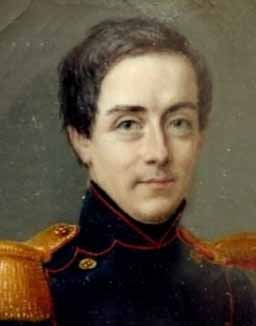
\includegraphics{complex/figures/pierre_laurent}
  \caption{Pierre Alphonse Laurent (1813–1854)}
\end{marginfigure}

This generalisation of a Taylor series in the presence of singularities is called a \emph{Laurent series}, in this case a Laurent series around the origin.


As an example, let's develop

$$f(z)=\frac{1}{z(z-1)}$$

in a Laurent series around the origin for the two rings $0 < | z | < 1$ and $ 1 < |z|$.

\begin{cue}
Do this first for the region where  $| z | < 1$, using the geometric series.
\end{cue}

For the first ring where $| z | < 1$, we can easily write

$$f(z)=\frac{1}{z} \cdot \frac{1}{z-1} = -\frac{1}{z} \sum_{m=0}^{\infty} z^m =-\frac{1}{z}-1-z-z^2 \cdots$$

However, in the second ring  $ 1 < |z|$, the previous series does not converge.

\begin{cue}
Divide the numerator and denominator of $f(z)$ by $z$, such that you can use the geometric series again.
\end{cue}

We can write

$$f(z)=\frac{1}{z} \cdot \frac{1 / z }{1-1/z} = \frac{1}{z^2} \sum_{m=0}^{\infty} \frac{1}{z^m} =\cdots+\frac{1}{z^4}+\frac{1}{z^3} + \frac{1}{z^2}$$

This series converges in the second ring, since $|1/z| < 1$ there.

\pagebreak

\begin{exer}
% difficulty: normal
% ugent
% youtube: 59Xeatg1Css
\label{ex_laurent_1}
Develop

$$f(z)=\frac{e^z}{z-1}$$

in a Laurent series around the origin for the ring $0 < | z | < 1$.

$e^z$ is a function which is analytic in all of $\mathbb{C}$ and defined by

$$e^z \stackrel{def}{=} \sum_{m=0}^{\infty} \frac{z^m}{m!} $$

Can you also think of a graphical representation that helps you take the product of the two series expansions? (It's helpful to look at the solution video here.)

\begin{sol}
$$f(z)= - \sum_{k=0}^{\infty} \left(\sum _{m=0}^k \frac{1}{m!} \right) z^k $$
\end{sol}

\end{exer}

\begin{exer}
  % difficulty: normal
  % youtube: Jo_c_zza3aA
  Same as Exercise \ref{ex_laurent_1}, but for the outer ring  $1 < | z |$.

\begin{sol}
$$f(z)=  \sum_{k=-\infty}^{\infty} \left(\sum_{m=k+1}^\infty \frac{1}{m!} \right) z^k $$
\end{sol}
  
\end{exer}

\begin{exer}
  % difficulty: normal
  % youtube: KRT-6y-UJjQ
  Show that you can change the radii of the contours used to derive the Laurent series, as long as they stay in the holomorphic region and keep their relative position with respect to $z$.

\end{exer}

\begin{exer}
  % difficulty: hard
  % youtube: _O9GqRJrZuM
  What is the relationship between a Fourier and a Laurent series?
  \begin{hnt}
  Transform a Fourier series in exponential notation to a Laurent series.
  \end{hnt}
\end{exer}


\pagebreak


\sectionugent{Singularities}

$z_0$ is a singular point of $f(z)$ if $f(z)$ is not analytic there. There are two important types of singularities, \emph{poles} and \emph{branch points}, which we will now discuss.

\subsection*{Poles}

We develop $f(z)$ in a Laurent series around $z_0$:

\begin{equation}
f(z)= \sum_{m=-\infty}^{\infty} a_m (z-z_0)^m
\end{equation} 

If the index $m$ doesn't run all the way to $-\infty$, but only to a finite value $-M$, $z_0$ is called a \emph{pole of order $M$}. As a trivial example, $f(z)=1/z$ has a pole of order 1 at $z=0$ (also called a \emph{simple pole}). $f(z)=1/z^2$ has a pole of order 2 at $z=0$

On the other hand, if there is an infinite number of negative $m$--values for which $a_m$ is non--zero, $z_0$ is called an \emph{essential singularity}.

\begin{cue}
  Verify by looking at the series expansion that $f(z)=e^{1/z}$ is an essential singularity.  
\end{cue}

Since

$$e^{1/z} = \sum_{m=0}^{\infty} \frac{1}{z^m m!} $$

has an infinite number of negative powers of $z$, it is an essential singularity.

Note that a pole of order $M$ can be removed by multiplying $f(z)$ by $(z-z_0)^M$. This obviously cannot be done for an essential singularity.

\noindent\marginnote{This is shown in Picard's Great Theorem.}One can also prove that in a small neighbourhood around an essential singularity, the function actually takes all possible complex values (with at most a single exception)! So, obviously it makes no sense to talk about the limit of that function there.

\pagebreak

\subsection*{Branch points}

Consider the relation

\begin{equation}
w = f(z) = z^{1/2} \label{eq-sqrt}
\end{equation}

(As a notational oddity, the complex square root is designated by the power $1/2$, to distinguish it from the real-valued square root.)

\begin{cue}
For a given value of $z$, how many solutions $w$ does the complex square root have? 
\end{cue}

For $z=\rho e^{j\theta}$, a possible solution to Eq.~\ref{eq-sqrt} is $w_1 = \rho^{1/2} e^{j\theta/2}$. However, there is a different point in the $w$--plane that corresponds to the same $z$, namely $w_2 = \rho^{1/2} e^{j(\theta/2+\pi)} = -w_1$. This is the complex analog of the real equation $y^2 = x$ for $x > 0$, which has two solutions $y = \pm \sqrt{x}$.

So, Eq.~\ref{eq-sqrt} is clearly not a single--valued function: a single point in the $z$--plane (except $z=0$) corresponds to two points in the $w$--plane. To get a handle on the multivaluedness of $z^{1/2}$, it's instructive to look at a graphical representation of this complex function. Since this is essentially a 4D--object, we can plot e.g. a 3D projection $(\Re(z),\Im(z),\Re(w))$ and use the phase of $w$ to colour the surface. This is done in Fig.~\ref{fig-riemann}.

\begin{marginfigure}[-3cm]
\centering
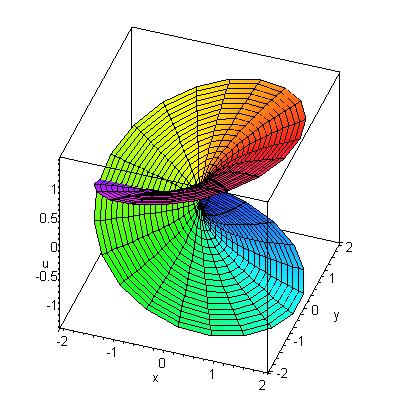
\includegraphics{complex/figures/riemann}
\caption{Riemann surface of $w=z^{1/2}$. Note that $u=\Re(w)$. }
\label{fig-riemann}
\end{marginfigure}

This 4D--object is also called the \emph{Riemann surface} of the complex square root function and Fig.~\ref{fig-riemann} shows a representation of it. It clearly shows the multivaluedness of the square root: for each point in the $z$--plane there are two points on the Riemann surface. Another way to appreciate this multivaluedness is by looking at how the argument of $w$ changes if we pick a point on the surface, make a full round trip on the Riemann surface, and arrive back at our original point.

\begin{cue}
When you do such an excursion in the complex plane, how does the angle of $w$ change? 
\end{cue}

From the figure, it is clear that we will have circled twice around the origin for that, so one could say that on the Riemann surface, the argument $w$ needs to change over $4 \pi$ in order to complete a full round trip. Therefore, this Riemann surface can be seen as an extension of the complex plane which is 'twice as large' as the regular complex plane.

Although the Riemann surface is a very profound and beautiful mathematical concept, for practical purposes people often like to work with single--valued functions mapping the complex plane to the regular (i.e. non-extended) complex plane. To do this, we can adopt a convention to restrict ourselves e.g. to values in the right half of the $w$--plane, i.e. where $\Re(w)>0$.


\begin{marginfigure}[-1cm]
\centering
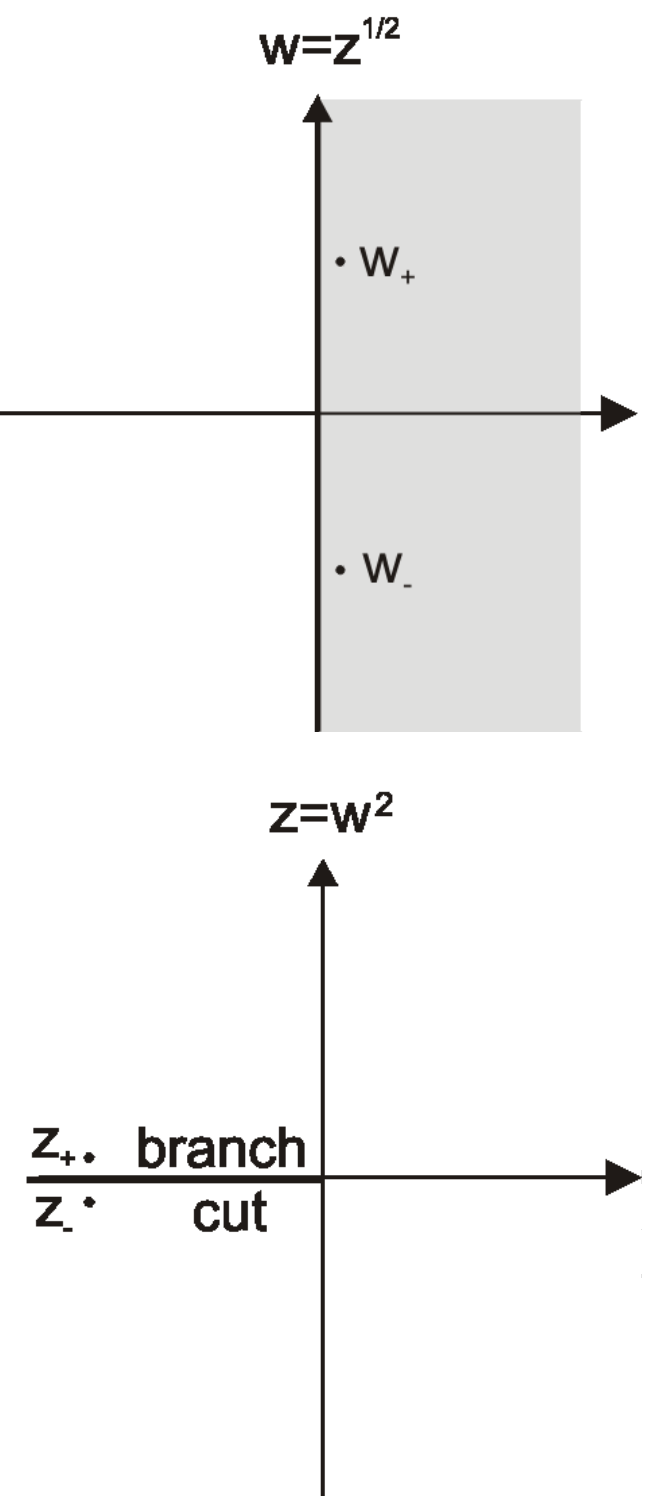
\includegraphics[width=4cm]{complex/figures/branchcut_portrait}
\caption{The mapping $w=z^{1/2}$.}
\label{fig-branchcut}
\end{marginfigure}


\begin{cue}
To which figure in the $z$--plane does the boundary $\Re(w)=0$ map?
\end{cue}

The boundary $\Re(w)=0$ between these two halves of the $w$--plane corresponds to the negative real axis in the $z$--plane. We call this negative real $z$--axis a \emph{branch cut}, originating from the \emph{branch point} $z=0$ (see Fig.~\ref{fig-branchcut}).

\begin{cue}
Looking at Fig.~\ref{fig-branchcut}, once we introduce the branch cut, what is the square root of $z_+$ and $z_-$? What happens to the output of the function if you cross the branch cut in the $z$--plane? 
\end{cue}

Our function is now no longer continuous when crossing the branch cut: for $z_+ = \rho e^{j (\pi - \epsilon)}$, we get $w_+ = \sqrt{\rho} e^{j (\pi/2 - \epsilon/2)}$, whereas for $z_- = \rho e^{j (\pi + \epsilon)}$, we get $w_- = \sqrt{\rho} e^{j (\pi/2 + \epsilon/2)} e^{j \pi}$. (This can be seen by looking at Fig.~\ref{fig-branchcut}.) In the limit of zero $\epsilon$, $w_+$ tends to $j\sqrt{\rho}$, whereas $w_-$ tends to $-j\sqrt{\rho}$.

\begin{marginfigure}[1cm]
\centering
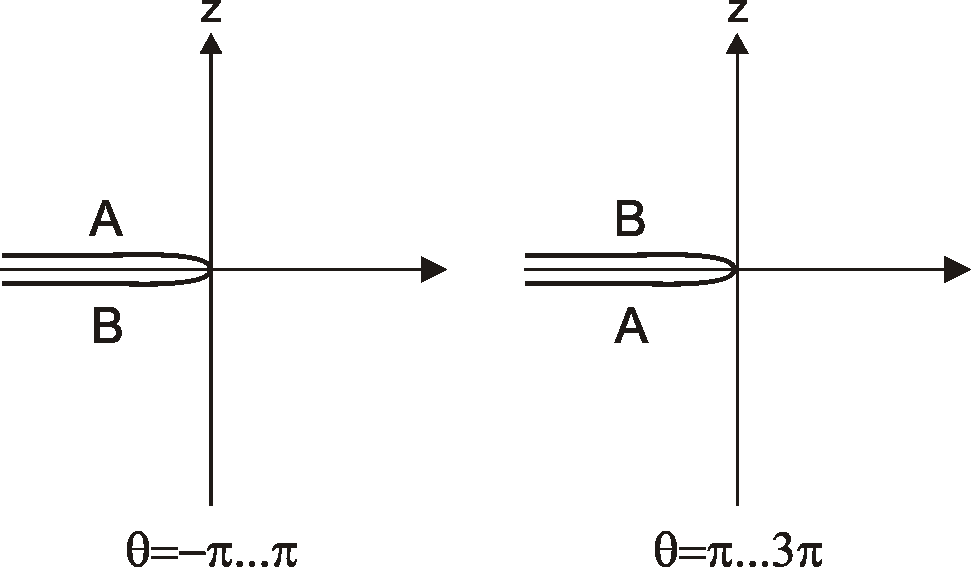
\includegraphics{complex/figures/sheets}
\caption{The branch cut cuts the Riemann surface in two separate Riemann sheets.
Adjacent regions on the Riemann surface are marked by the same letters.}
\label{fig-sheets}
\end{marginfigure}

The relationship between branch cuts and the Riemann surface is show schematically in Fig.~\ref{fig-sheets}: our branch cut cuts the Riemann surface in two separate \emph{Riemann sheets}, one corresponding to arguments $[-\pi, \pi]$, the other one corresponding to arguments $[\pi,3 \pi]$.

It is important to remark that, when choosing a contour to evaluate the integral theorems we've seen so far, we are not allowed to cross a branch cut, as the resulting discontinuity would make the function no longer analytic. However, skirting on one edge of a branch cut, circling around the branch point and returning along the other edge is allowed, as the function stays continuous and analytic throughout the entire path. 

Note that integrals on both sides of a branch cut will generally not cancel out, unlike integrals on both sides of the contour cut in Fig.~\ref{fig-cauchy-II}, which only serves to transform a contour into one which can be used to apply Cauchy's theorem.

The choice of branch cut is in no way unique: any line (even a curved one) from $z=0$ to infinity would suit the purpose equally well. Its only goal is to lift the ambiguity with respect to the choice of $w$. There are however often physical reasons which inspire the choice of branch cut.

\pagebreak

\begin{exer}
% difficulty: normal
% ugent
% youtube: 6ecPpRUTieg
\label{ex-branch-ang}
Show that asking that $\Re(w)>0$ is equivalent to asking that you restrict the angle of $z$ to $[-\pi, \pi]$ before halving it to calculate the square root. Do this by looking at 4 strategically located points in the $z$-plane (just above/below the positive/negative real axis). Write down their angles, and then see what the corresponding angles in the $w$--plane are. Are the results in the correct half plane? Verify that crossing the branch cut leads to a discontinuity. (It's helpful to look at the solution video here.)
\end{exer}

\begin{exer}
% difficulty: normal
% ugent
% youtube: y-F1acXHgAk
\label{ex-product-roots}
\begin{marginfigure}[0.5cm]
\centering
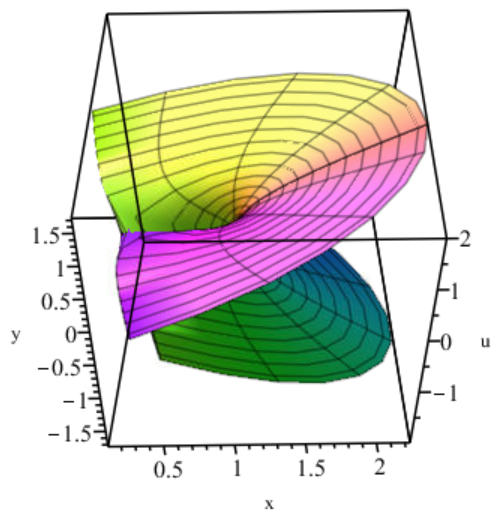
\includegraphics[width=4cm]{complex/figures/riemann2}
\caption{Half the Riemann surface of $w=(z-1)^{1/2}(z+1)^{1/2}$. Note that $u=\Re(w)$. }
\label{fig-riemann2}
\end{marginfigure}
Consider

$$f(z)=(z-1)^{1/2}(z+1)^{1/2}$$

Using the conventional choice of branch cut for an individual square root (expressed in terms of angles as in Ex.~\ref{ex-branch-ang}), show that the branch cut for this product of square roots is the segment $-1 \le x \le 1$. Do this by looking at 8 strategically located points in the $z$--plane, and calculate the angle of the corresponding $w$--value.


Verify that it is possible to establish a single--valued function using this cut, and that any contour which does not cross this cut does not encounter discontinuities.
\end{exer}

\begin{exer}
  % difficulty: normal
  % youtube: 2jV5xidyl2o
How many sheets does the Riemann surface of $w=\ln(z)$ have?
\end{exer}

\begin{exer}
  % difficulty: hard
  % youtube: siBBZMkJrB8
\begin{marginfigure}[0.cm]
\centering
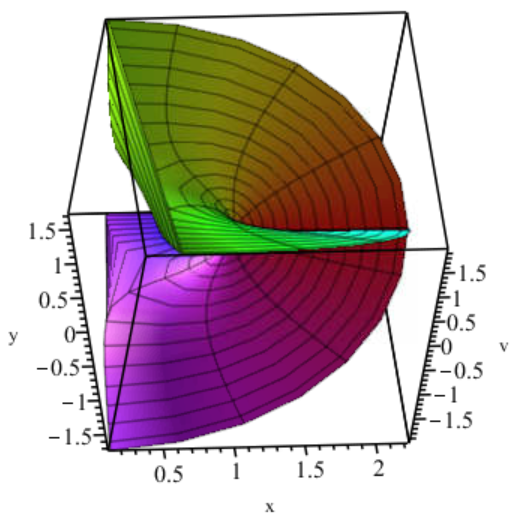
\includegraphics[width=4cm]{complex/figures/riemann3}
\caption{Half the Riemann surface of $w=(z-1)^{1/2}(z+1)^{1/2}$. Note that $v=\Im(w)$. }
\label{fig-riemann3}surf
\end{marginfigure}

For Eq.~\ref{ex-product-roots}, what range of angles would you need to chose for the arguments of each of the square roots in order to end up with a branch cut consisting of the union of  $x \le -1$ and $1 \le x$?


Note that Fig.~\ref{fig-riemann2} and \ref{fig-riemann3} each seem to suggest a different natural choice for a branchut, even though they both correspond to the same Riemann surface.


Why is that? Which branch cut is more natural?
  \begin{sol}
    $\arg(z-1) \in [0, 2 \pi], \arg(z+1) \in [-\pi,\pi]$. Figs.~\ref{fig-riemann2} and \ref{fig-riemann3} are both different projections of a 4D Riemann surface. That they seem to suggest a certain natural choice for the branchcut is purely accidental.
\end{sol}
\end{exer}

\pagebreak


\sectionugent{Residue calculus}

One of the main goals of this chapter is to provide you with a powerful way of calculating some real-valued integrals by transforming them to complex contour integrals, and solve them using straightforward algebra, as opposed to using tricky calculus. An important ingredient in this recipe is the use of so-called \emph{residue calculus}.

\subsection*{Residue}

Suppose $z_0$ is an isolated singularity of $f(z)$. We can develop this function in a Laurent series around $z_0$:

\begin{equation}
f(z)= \sum_{m=-\infty}^{\infty} a_m (z-z_0)^m
\end{equation} 

The \emph{residue} of $z_0$ is defined as $a_{-1}$, i.e. the coefficient of $1/z$ in the Laurent series. Using Eq.~\ref{eq-laurent-int}, we immediately get

\begin{equation}
\mathrm{Res}_{z_0}=\frac{1}{2 \pi j }  \oint_{{C}} f(z) dz \label{eq-res-int}
\end{equation}

\begin{cue}
  By looking at their series expansion, calculate the residues of the following functions at $z=0$.
  $$\begin{array}{lcll}a) & f(z)=1/z \\b) & f(z)=1/z^2 \\c) & f(z)=e^{1/z}\end{array}$$
\end{cue}

For $f(z)=1/z$ and $f(z)=1/z^2$, the series expansion is the function itself, so we can quickly see that the residues are 1 and 0 respectively.

$z=0$ is an essential singularity of $f(z)=e^{1/z}$ with residue 1, since

$$e^{1/z} = \sum_{m=0}^{\infty} \frac{1}{z^m m!} $$

\begin{exer}
  % difficulty: trivial
  % youtube: 3yTQUc3fZSU
  Integrate the Laurent series around a singularity term-by-term. What formula do you recover?
\end{exer}

\begin{exer}
  % difficulty: normal
  % youtube: B5Il6eMovPg
  Use a series expansion to calculate the residue at $z=0$ of
  $$z \cos \frac{1}{z}$$
  \begin{sol}
    $$-1/2$$
  \end{sol}
\end{exer}

\begin{exer}
  % difficulty: normal
  % youtube: IZGlLE09wOQ
  Use a series expansion to calculate the residue at $z=0$ of

  $$\frac{z - \sin z}{z}$$
  \begin{sol}
    $$0$$
  \end{sol}
\end{exer}


\subsection*{Residue theorem}

Suppose $f(z)$ is analytic inside a contour ${C}$, except for some isolated singularities $z_k$ inside ${C}$ (so, branch cuts are not allowed, but e.g. poles are OK). Then

\begin{equation}
\fbox{$\displaystyle
\oint_{{C}} f(z) dz = 2 \pi j \sum_k \mathrm{Res}_{z_k} \label{eq-res-theorem}
$}
\end{equation} 

The summation index $k$ runs over all singularities enclosed by the contour. Note that no singularity should lie on the contour itself.

\begin{marginfigure}
\centering
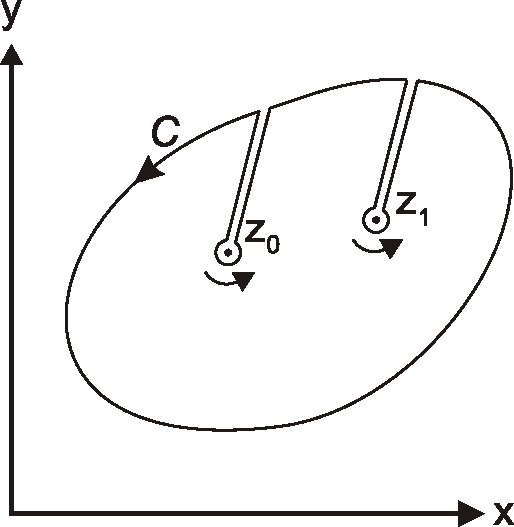
\includegraphics{complex/figures/residue}
\caption{Contour to prove residue theorem.}
\label{fig-residue}
\end{marginfigure}

To prove Eq.~\ref{eq-res-theorem}, we make use of the contour in Fig.~\ref{fig-residue}.

\begin{cue}
  Apply Cauchy's theorem on this contour. Then, use the relation between the residue and a contour integral around the singularity (Eq.~\ref{eq-res-int}) to prove the residue theorem. 
\end{cue}

Applying Cauchy's theorem on this contour (the straight segments cancel as before):

\begin{equation}
\oint_{{C}} f(z) dz - \sum_k \oint_{{C}_k} f(z) dz = 0
\label{eq-res-proof-1}
\end{equation}

The integral around any singular point can be written as (Eq.~\ref{eq-res-int})

\begin{equation}
\oint_{{C}_k} f(z) dz = 2 \pi j \mathrm{Res}_{z_k} \label{eq-res-proof-2}
\end{equation} 

Combining Eq.~\ref{eq-res-proof-1} and Eq.~\ref{eq-res-proof-2} immediately proves the theorem.

\subsection*{Calculating residues}

The residue theorem is of enormous practical importance, as it allows us to replace the cumbersome problem of evaluating contour integrals by the algebraic problem of calculating residues at enclosed singular points. Because of its importance, we will now discuss a number of techniques that allow us to easily calculate the residues, apart from writing down the Laurent series, or applying Eq.~\ref{eq-res-int}. The proofs are left as an exercise. The formulas for the case of a single pole are worth memorising.

\begin{exer}
% difficulty: normal
% ugent
% youtube: eeAa-wZ2iDc
  If $z_0$ is a simple pole of $f(z)$, use the Laurent series to prove that
  $$\mathrm{Res}_{z_0} = \left[f(z)(z-z_0)\right]_{z=z_0}$$

  (Explicitly writing down the first few terms of the Laurent series makes this slightly easier to solve.)
  
\label{ex-res1}
\end{exer}

\begin{exer}
  % difficulty: trivial
  % youtube: UUbcQvMs134
  Calculate the residue at $z=0$ of

   $$\frac{1}{z+z^2}$$ 
\begin{sol}
  $$1$$
\end{sol}
\end{exer}

\begin{exer}
% difficulty: hard
% ugent
% youtube: rVRDlqpRcxk
  If $z_0$ is a simple pole of $f(z)=\frac{g(z)}{h(z)}$, i.e. $z_0$ is a simple zero of $h(z)$ and $g(z_0) \ne 0$, show that
    $$\mathrm{Res}_{z_0} = \frac{g(z_0)}{h'(z_0)}$$
\begin{hnt}
Write $h(z)$ as $r(z)(z-z_0)$, and apply the result from Ex.~\ref{ex-res1}.
\end{hnt}
\end{exer}

\begin{exer}
  % difficulty: hard
  % youtube: LQNlwXZKlQo
If $z_0$ is a pole of order $M$ of $f(z)$, prove that
$$\mathrm{Res}_{z_0} = \frac{1}{(M-1)!}{\left[\frac{d^{M-1}}{dz^{M-1}}[f(z)(z-z_0)^M]\right]}_{z=z_0}$$
\end{exer}


\pagebreak


\sectionugent{Limit theorems}
\label{week2}

Sometimes, we are dealing with contours that are infinitely large or infinitely small. For these cases, the following limit theorems (which we will present mostly without proof) are of great practical importance.

\subsection*{Jordan's lemma}

\begin{marginfigure}
\centering
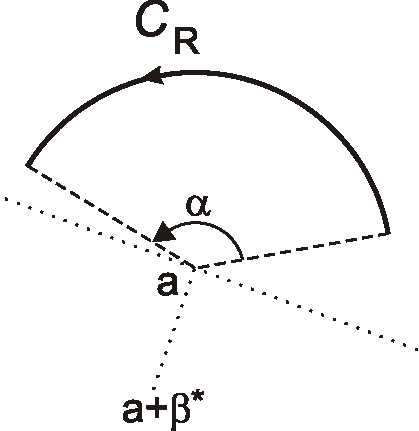
\includegraphics[width=4cm]{complex/figures/jordan}
\caption{Jordan's lemma.}
\label{fig-jordan}
\end{marginfigure}

Jordan's lemma deals with integrals along a circular path  (see Fig.~\ref{fig-jordan}) containing a complex exponential: 

$$ \int_{{C}_R} f(z) e^{\beta z} dz$$

Note that here (and also for the next limit theorems) ${{C}_R}$ only includes the circular part of the contour and not the straight line segments.

Under which circumstances does this integral go to zero if the radius $R$ goes to infinity? It seems reasonably that both factors of the integrand should go to zero for that. However, the exponential does not go to zero at infinity everywhere in the complex plane. 

\begin{cue}
Show that if $b>0$, then $e^{jbz}$ goes to zero if $z$ goes to infinity, but only in the upper half plane.
\end{cue}

It can be shown that in general, for a contour lying on the 'proper' side of $a$, i.e. the half plane not containing $a+\beta^*$ (see Fig.~\ref{fig-jordan}), we have that if

\begin{marginfigure}[-2.5cm]
  % credits: Wikipedia
  % url: https://en.wikipedia.org/wiki/Camille_Jordan
  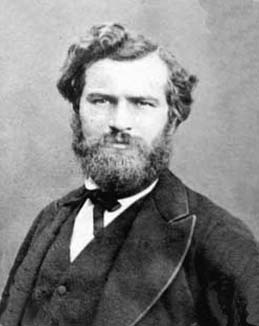
\includegraphics{complex/figures/camille_jordan}
  \caption{Camille Jordan (1838–1922) }
\end{marginfigure}

\begin{equation}
\lim_{z \to \infty} f(z) = 0
\end{equation}
then
\begin{equation}
\lim_{R \to \infty} \int_{{C}_R} f(z) e^{\beta z} dz = 0
\end{equation}

\begin{cue}
Verify that the construction of the 'proper' half plane reduces to the upper half plane in case $a=0$ for $ \int_{{C}_R} f(z) e^{jb z} dz$ with $b>0$.
\end{cue}

\subsection*{Big limit theorem}

For a circular contour spanning an angle $\alpha$ with top at $z=a$ (see Fig.~\ref{fig-limit-theorem}), we have that if

\begin{equation}
\lim_{z \to \infty}  f(z) (z-a) = A
\end{equation}
then
\begin{equation}
\lim_{R \to \infty} \int_{{C}_R} f(z) dz = j \alpha A
\end{equation}

\begin{marginfigure}
\centering
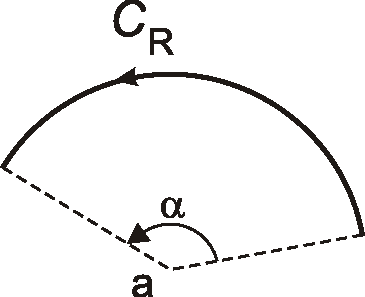
\includegraphics[width=3.5cm]{complex/figures/limit_theorem}
\caption{Contours for big and small limit theorems.}
\label{fig-limit-theorem}
\end{marginfigure}

Important: do not confuse when to use Jordan's lemma and when to use the big limit theorem (look for the presence of an exponential). Also do not confuse when to add a factor $z-a$ to the limit related to $f(z)$.

\subsection*{Small limit theorem} 

For a circular contour spanning an angle $\alpha$ with top at $z=a$ (see Fig.~\ref{fig-limit-theorem}), we have that if

\begin{equation}
\lim_{z \to a}  f(z) (z-a) = A
\end{equation}
then
\begin{equation}
\lim_{R \to 0} \int_{{C}_R} f(z) dz = j \alpha A
\end{equation}

\begin{exer}
  % difficulty: hard
  % youtube: kv1-JzPvAwI
  Prove the small limit theorem for the special case where $f(z)$ has a single pole at $z=a$.
  \begin{hnt}
    Integrate the Laurent series term by term.
  \end{hnt}
\end{exer}

\subsection*{Cauchy principal value}

\begin{marginfigure}
\centering
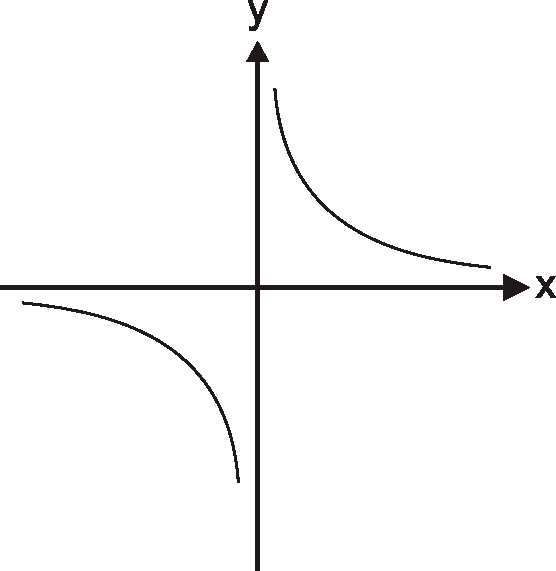
\includegraphics[width=4cm]{complex/figures/pv}
\caption{The function $1/x$.}
\label{fig-pv}
\end{marginfigure}

Let's discuss a final technicality that will come handy in some cases. Consider the integral $\int_0^1 dx / x$ (see Fig.~\ref{fig-pv}). As the area under this curve is infinite, this integral clearly diverges.

Strictly speaking, the same is true for the integral $\int_{-1}^1 dx / x$, as this should be seen as

\begin{equation}
\lim_{\epsilon_1 \to 0} \int_{-1}^{-\epsilon_1} \frac{dx}{x} + \lim_{\epsilon_2
\to 0} \int_{\epsilon_2}^1 \frac{dx}{x}
\end{equation}  

because each term separately diverges, and the limits are taken independently. However, Fig.~\ref{fig-pv} suggests that both singularities will cancel out. Mathematically, this means that

\begin{equation}
\lim_{\epsilon \to 0} \int_{-1}^{-\epsilon} \frac{dx}{x} + \lim_{\epsilon \to 0}
\int_{\epsilon}^1 \frac{dx}{x} = 0 \label{eq-pv}
\end{equation}  

if both limits are taken at the same time. This is written succinctly as

\begin{equation}
PV \int_{-1}^1 \frac{dx}{x} = 0
\end{equation} 

where $PV$ stands for the Cauchy \emph{principal value} and represents the balancing process of Eq.~\ref{eq-pv}. However, $\int_{-1}^1 dx / x$ still diverges.

The same balancing process can also be applied to limits at infinity:

\begin{equation}
PV \int_{-\infty}^\infty f(x) dx = \lim_{a \to \infty} \int_{-a}^{a} f(x) dx
\end{equation} 

\pagebreak

\sectionugent{Evaluation of real--valued integrals}

Now we have all the necessary tools in our box to tackle the important problem
of calculating real--valued integrals by means of complex contour integration.
We will present a number of examples which illustrate some typical techniques
used in this respect.

\subsection*{Example 1: integrals of the type $\int_0^{2 \pi} f(\cos \theta, \sin \theta) d \theta$}

Consider integrals of the type

\begin{equation}
\int_0^{2 \pi} f(\cos \theta, \sin \theta) d \theta \label{eq-cont-int-1}
\end{equation} 

By letting $z=e^{j \theta}$, we get 

\begin{equation}
\cos \theta = \frac{z + 1/z}{2}
\end{equation} 

\begin{equation}
\sin \theta = \frac{z - 1/z}{2j}
\end{equation} 

\begin{equation}
d \theta = \frac{1}{j}\frac{dz}{z}
\end{equation} 

such that the integral Eq.~\ref{eq-cont-int-1} becomes

\begin{equation}
-j \oint_{{C}} f\left(\frac{z + 1/z}{2}, \frac{z - 1/z}{2j}\right)
\frac{dz}{z}
\end{equation} 

The integration contour ${C}$ is the unit circle, and the integral can easily be evaluated using the residue theorem.

As an example, we will calculate

\begin{equation}
I = \int_0^{2 \pi} \frac{d \theta}{1 + \epsilon \cos \theta}, \hspace{0.5cm}
|\epsilon| < 1
\end{equation} 

\begin{cue}
  Transform this to a complex contour integral.
\end{cue}

This transforms into

\begin{equation}
I = -j \oint_{{C}} \frac{1}{1 + (\epsilon / 2)\left(z + 1/z\right)}
\frac{dz}{z}
\end{equation} 

or

\begin{equation}
I = -\frac{2j}{\epsilon} \oint_{{C}} \frac{dz}{z^2 + (2 / \epsilon)z +
1}
\end{equation} 

\begin{cue}
  Where are the poles of this function? Calculate the relevant residues.
\end{cue}

The poles of this function are

\begin{equation}
z = - \frac{1}{\epsilon} \pm \frac{1}{\epsilon} \sqrt{1 - \epsilon^2}
\end{equation} 

Only the pole with the plus sign lies within the unit circle, as can be verified e.g. by a series expansion for small values of $\epsilon$. By using the formula from Ex. \ref{ex-res1} to calculate the residue there, we get

\begin{equation}
I = -\frac{2j}{\epsilon} \cdot 2 \pi j \left[\frac{1}{z - (-\frac{1}{\epsilon} -
\frac{1}{\epsilon} \sqrt{1 - \epsilon^2})}\right]_{z = - \frac{1}{\epsilon} +
\frac{1}{\epsilon} \sqrt{1 - \epsilon^2}}
\end{equation}

or

\begin{equation}
I = -\frac{2j}{\epsilon} \cdot 2 \pi j \cdot \frac{1}{\frac{2}{\epsilon} \sqrt{1
- \epsilon^2}}
\end{equation}

\begin{cue}
  Combine everything to calculate the original integral.
\end{cue}

So finally

\begin{equation}
\int_0^{2 \pi} \frac{d \theta}{1 + \epsilon \cos \theta} = \frac{2 \pi}{\sqrt{1
- \epsilon^2}}, \hspace{0.5cm} |\epsilon| < 1
\end{equation} 

\pagebreak
\subsection*{Example 2: integrals of the type $\int_\infty^{\infty} f(z) e^{jbz} dz$}

Let's calculate

\begin{equation}
\int_0^{\infty}\frac{\cos \lambda x}{1 + x^2} dx, \hspace{0.5cm} \lambda > 0
\end{equation}

\noindent\marginnote{Alternatively, we could have made use of $\cos z = (e^{j z} + e^{-jz})/2$, but then Jordan's lemma would have required two separate integrals for each of the complex exponentials, each with a different contour.}To do this, we will calculate the real part of the following contour integral (Fig.~\ref{fig-example-2}):

\begin{equation}
I = \oint_{{C}} \frac{e^{j \lambda z}}{1 + z^2} dz
\end{equation}

\begin{marginfigure}
\centering
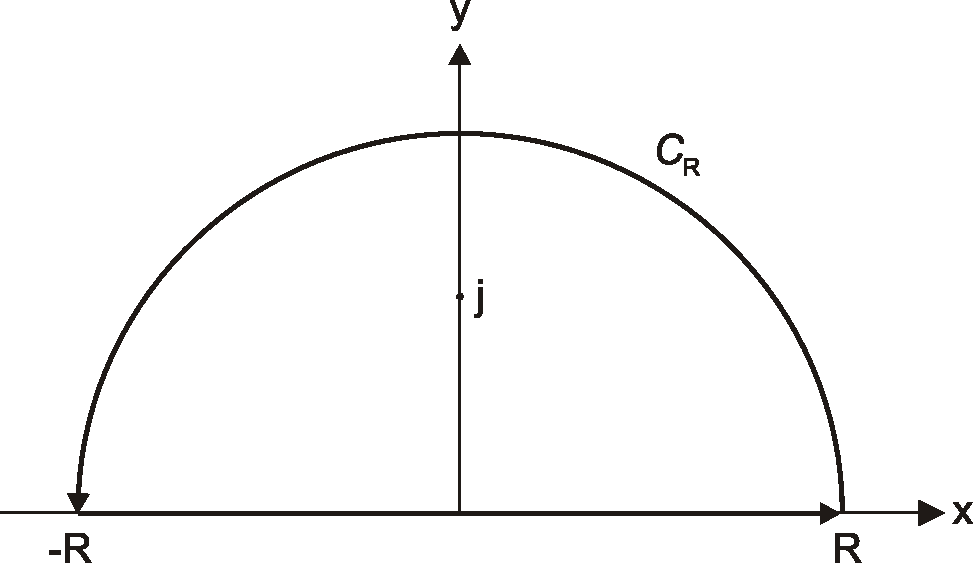
\includegraphics{complex/figures/int_ex_2}
\caption{Contour for example 2.}
\label{fig-example-2}
\end{marginfigure}

Evaluating the part of this contour on the positive real axis, and then taking the real part will recover the required cosine in the integral. It is true that we are only interested in the contribution from the positive real axis, but as you'll see, we'll be able to deal with the other contributions in due course.

\begin{cue}
Use residue calculus to evaluate the contour integral.
\end{cue}

The only pole enclosed by the contour is at $j$, with residue $e^{-\lambda}/(j+j)$, such that the residue theorem leads to

\begin{equation}
\int_{-R}^{R} \frac{e^{j \lambda x}}{1 + x^2} dx + \int_{{C_R}}
\frac{e^{j \lambda z}}{1 + z^2} dz = 2 \pi j \frac{e^{-\lambda}}{2 j} = \pi
e^{-\lambda}
\end{equation}

Let's now take the limit $R \to \infty$ and study the different contributions to the contour.

\begin{cue}
Can we apply Jordan's lemma to ${C_R}$? 
\end{cue}

If $\lambda > 0$, the contour lies indeed in the 'proper' part of the complex plane. For the second condition, we need to calculate the following limit:

\begin{equation}
\lim_{z \to \infty}\frac{1}{1+z^2} = \lim_{z \to \infty}\frac{1}{1+|z|^2 e^{2 j
\arg z}}
\end{equation}

Since $e^{2 j \arg z}$ always stays bounded, this limit goes to zero for all directions in the complex plane. So, we can apply Jordan's lemma and the contribution from ${C_R}$ vanishes.

\begin{cue}
Write down what remains of the contour integral and use this to calculate our original real-valued integral.
\end{cue}

\begin{equation}
\int_{-\infty}^{\infty}\frac{e^{j \lambda x}}{1 + x^2} dx = \pi e^{-\lambda}
\end{equation}

\noindent\marginnote{Only for readers that like to lie awake at night about mathematical rigour: strictly speaking, you should take the real part \emph{before} taking the limit $R \to \infty$. Can you see why?}After taking the real part of the result, we get

\begin{equation}
\int_{-\infty}^{\infty}\frac{\cos \lambda x}{1 + x^2} dx = \pi e^{-\lambda}
\end{equation}

Finally, due to the even character of the integrand, we arrive at

\begin{equation}
\int_0^{\infty}\frac{\cos \lambda x}{1 + x^2} dx = \frac{\pi}{2} e^{-\lambda}
\end{equation}

\subsection*{Example 3: integrals with branch cuts}

Let's now try an example with branch point singularities:

\begin{equation}
\int_0^{\infty}\frac{\sqrt{x}}{x^2+a^2}dx, \hspace{0.5cm} a > 0
\end{equation}

\begin{marginfigure}[-0cm]
\centering
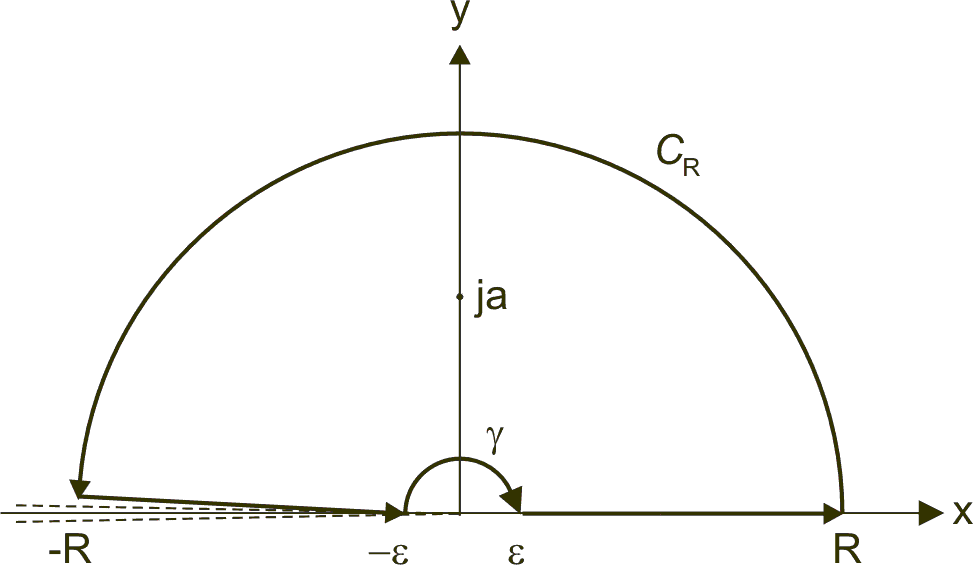
\includegraphics{complex/figures/int_ex_3}
\caption{Contour for example 3.}
\label{fig-example-3}
\end{marginfigure}

We stick to the traditional choice of branch cut, namely the negative real axis (Fig.~\ref{fig-example-3}). The contour is placed 'just above' this branch cut. In order to avoid the branch point at $z=0$, we also make a small detour around the origin.

\begin{cue}
Use residue calculus to evaluate the contour integral.
\end{cue}

\begin{align}
I = \oint_{{C}} \frac{z^{1/2}}{z^2+a^2} dz =& \, 2 \pi j \textrm{Res}_{j a}
\nonumber \\
=& \, 2 \pi j \frac{(j a)^{1/2}}{ja + ja} \nonumber \\
=& \, \pi \frac{\sqrt{a}e^{\frac{1}{2}j\frac{\pi}{2}}}{a} \nonumber \\
=& \, \frac{\pi}{\sqrt{a}} e^{j \pi /4}
\end{align}

\begin{cue}
What is the contribution of ${C_R}$ to the integral in the limit of infinite radius?
\end{cue}

We use the big limit theorem to calculate the contribution of the outer circular part ${C_R}$ to the integral. For that, we calculate the following limit:

\begin{equation}
\lim_{z \to \infty}\frac{z^{1/2}}{z^2+a^2} \cdot z = \lim_{z \to
\infty}\frac{\sqrt{|z|}e^{j \arg z / 2}}{|z|^2 e^{2 j \arg z}+a^2} \cdot |z|
e^{j \arg z}
\end{equation}

Just as before, the complex exponentials involving $\arg z$ always stay bounded, so this limit goes to zero and the contribution from this part of the contour vanishes.

\begin{cue}
What is the contribution of the small inner circle $\gamma$ to the integral in the limit of zero radius?
\end{cue}

Similarly, we use the small limit theorem to show that the contribution for the semicircle around the branch point vanishes in the limit of zero radius:

\begin{equation}
\lim_{z \to 0}\frac{z^{1/2}}{z^2+a^2} \cdot z = \frac{0}{a^2} = 0
\end{equation}

\begin{cue}
Write down what remains of the contour integral and use this to calculate our original real-valued integral.
\end{cue}

So finally we are left with

\begin{equation}
I = \int_{- \infty}^{0}\frac{z^{1/2}}{z^2+a^2}dz + \int_{0}^{\infty}\frac{z^{1/2}}{z^2+a^2}dz
\end{equation} 

Returning from $z$ to $x$, we get with our choice of branch cut (see the calculation of $w_+$ in the section on branch cuts) that 

\begin{equation}
z^{1/2} = 
\begin{cases}
\sqrt{x}, & x > 0\\
j \sqrt{-x}, & x < 0
\end{cases}
\end{equation} 

such that

\begin{align}
I = & \int_{- \infty}^{0}\frac{j\sqrt{-x}}{x^2+a^2}dx +
\int_{0}^{\infty}\frac{\sqrt{x}}{x^2+a^2}dx \nonumber \\
 = & \, (1 + j) \ \int_{0}^{\infty}\frac{\sqrt{x}}{x^2+a^2}dx \nonumber \\
 = & \, \frac{\pi}{\sqrt{a}} e^{j \pi /4}
\end{align} 

So finally

\begin{equation}
\int_0^{\infty}\frac{\sqrt{x}}{x^2+a^2}dx = \frac{\pi}{\sqrt{2a}}
\end{equation}

\begin{exer}
% difficulty: trivial
% ugent
% youtube: v09NSxfVNY0
  \label{ex-contour-integral-1}
Use complex contour integration to calculate
$$\int_0^{\infty} \frac{dx}{1+x^2}$$
\begin{sol}
$$\frac{\pi}{2}$$
\end{sol}
\end{exer}

\begin{exer}
  % difficulty: trivial
  % youtube: YhbD-ye_RTE
Repeat Ex.~\ref{ex-contour-integral-1}, but show that you get the same result if you close the contour in a different half plane.
\end{exer}

\begin{exer}
% difficulty: trivial
% ugent
% youtube: 3RJv9Nf1lts
  Comment on the suitability of the following contours for calculating
  $$ \int_0^{\infty} \frac{\sin x}{x} dx$$

  (All of these were harvested from actual students trying their hand at this problem.)

\begin{center}
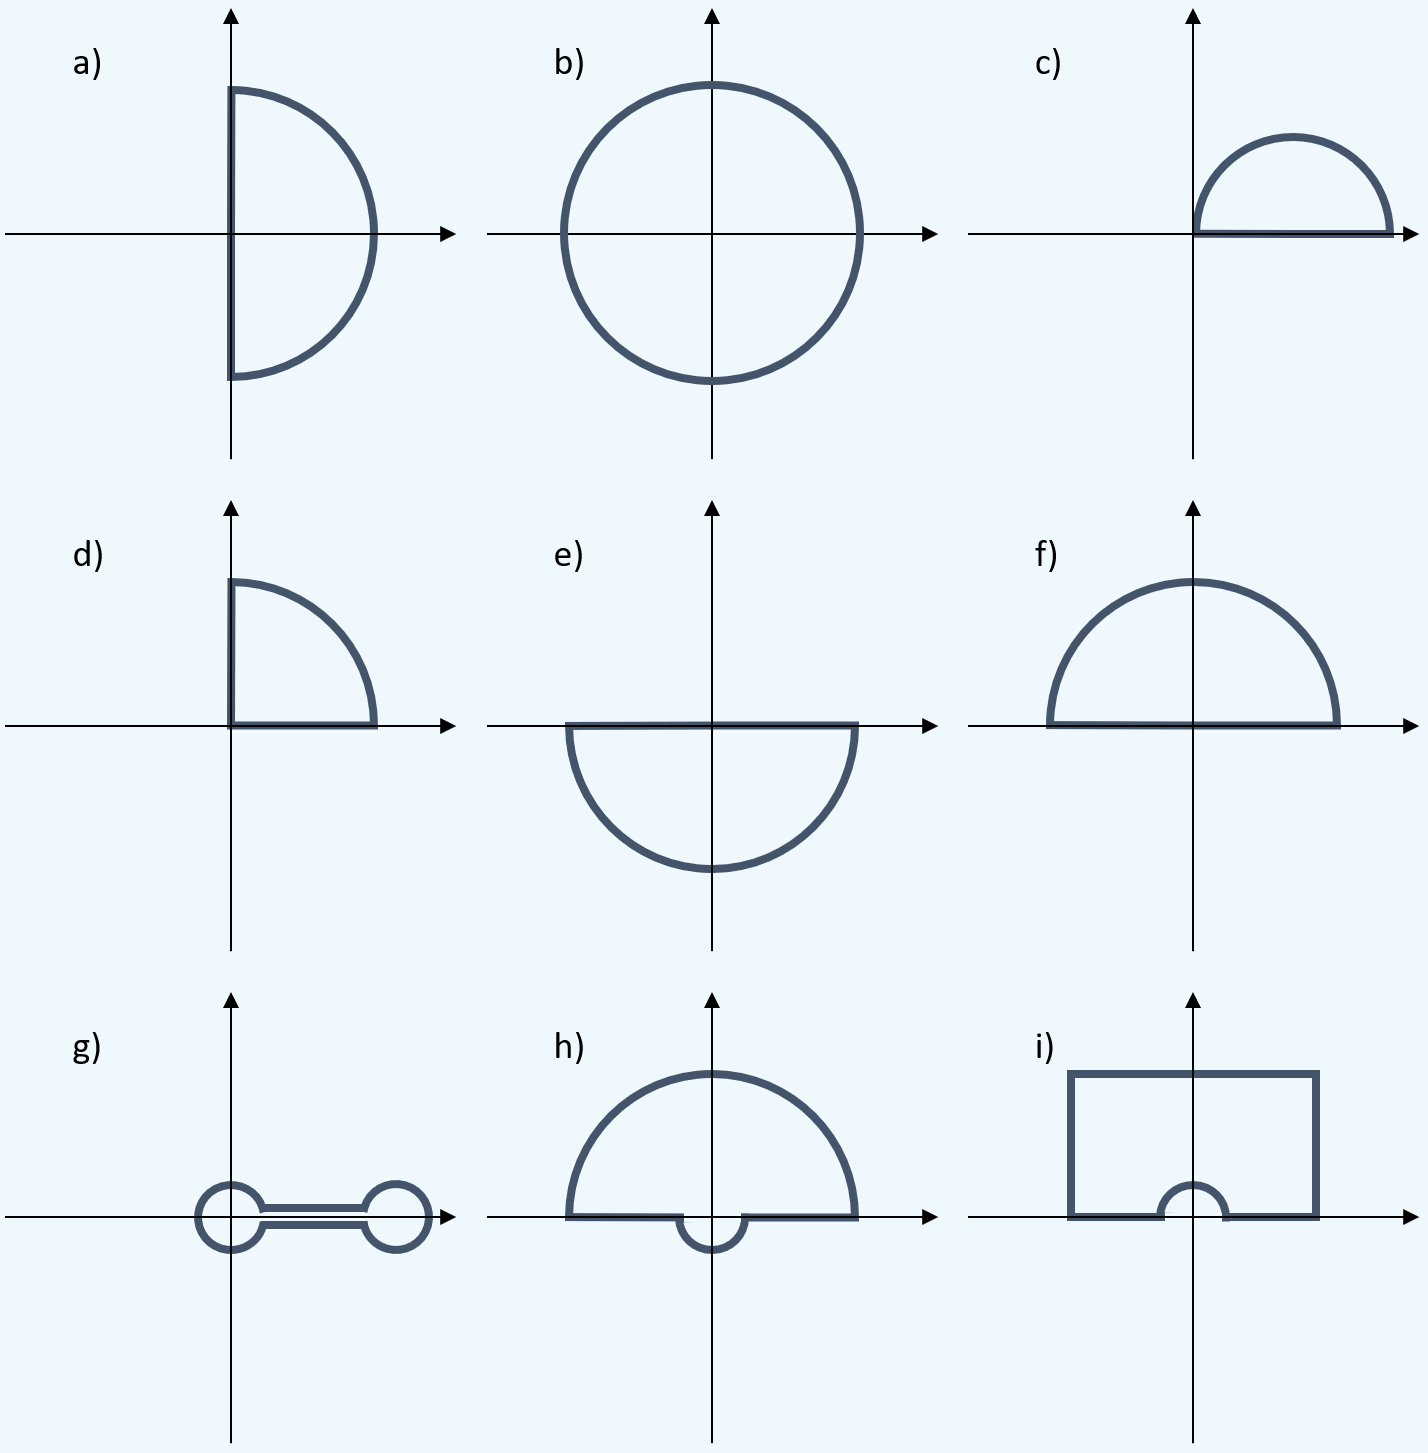
\includegraphics[width=10cm]{complex/figures/contours}
\end{center}
  
\end{exer}

\begin{exer}
% difficulty: normal
% ugent
% youtube: _DBoH63WDGk 
Use complex contour integration to calculate
$$ \int_0^{\infty} \frac{\sin x}{x} dx$$
\begin{sol}
$$\frac{\pi}{2}$$
\end{sol}
\end{exer}

\begin{exer}
  % difficulty: normal
  % youtube: 46bqZ-w-rSI
Use complex contour integration to calculate
$$ \int_0^{\infty} \frac{1}{\left(x^2 + a^2\right)^2} dx$$
Here $a$ is a positive real-valued number.
\begin{sol}
$$\frac{\pi}{4 a^3}$$
\end{sol}
\end{exer}

\begin{exer}
  % difficulty: normal
  % youtube: tQnHZ3Oa4XI
Use complex contour integration to calculate
$$ \int_{-\infty}^{\infty} \frac{\sin \pi x}{x (x-1) (x-2)} dx$$
\begin{sol}
$$2 \pi$$
\end{sol}
\end{exer}

\begin{exer}
  % difficulty: normal
 % youtube: PudvMdmpljw 
Use complex contour integration to calculate
$$ \int_0^{2\pi} \frac{\cos^2 \theta d \theta}{13-5\cos 2 \theta}$$
\begin{sol}
$$\frac{\pi}{10}$$
\end{sol}
\end{exer}

\begin{exer}
  % difficulty: hard
  % youtube: K6vOAX72XwM 
Use complex contour integration to calculate
$$ \int_0^\pi \sin^{2n} \theta d \theta$$
Here, $n \ge 1$.
\begin{sol}
$$\frac{(2n)!}{ 2^{2n}(n!)^2} \pi$$
\end{sol}
\end{exer}

\begin{exer}
  % difficulty: hard
  % youtube: xwUzDDkHVnY
Use complex contour integration to calculate
$$ \int_0^\infty \frac{x ^ {2m}}{x^{2n} + 1} dx$$
Here $m$ and $n$ are integers and $0 \le m < n$.
\begin{sol}
$$\frac{\pi}{2n} \mathrm{cosec} \left( \frac{2m+1}{2n} \pi \right)$$
\end{sol}
\end{exer}


\pagebreak


\sectionugent{Application: Kramers--Kronig dispersion relations}

Suppose $f(z)$ is an analytic function with $\lim_\infty f(z) = 0$ in the upper half of the complex plane.

\begin{marginfigure}[-0.5cm]
\centering
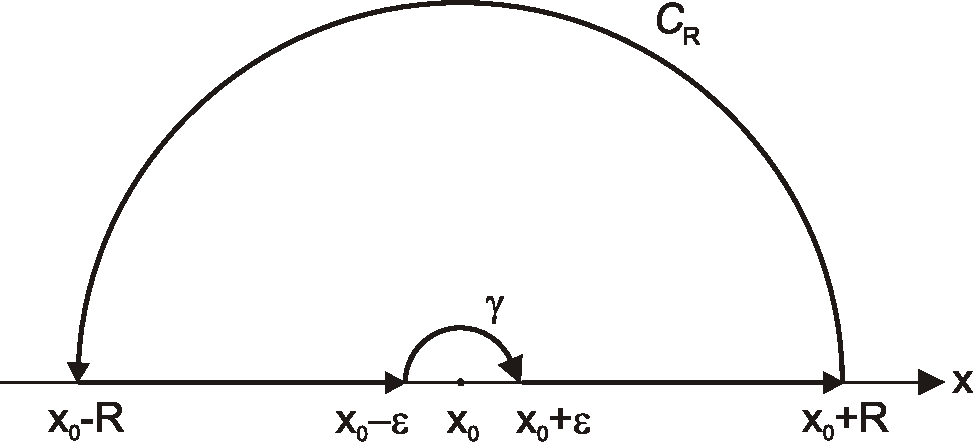
\includegraphics{complex/figures/kk}
\caption{Contour for Kramers--Kronig dispersion relations.}
\label{fig-KK}
\end{marginfigure}

Applying Cauchy's theorem to the contour in Fig.~\ref{fig-KK} leads to

\begin{equation}
\oint_{{C}} \frac{f(z)}{z-x_0} dz = 0
\end{equation}

\begin{cue}
Split up the contour integral into contributions from its different parts.
\end{cue}

\begin{marginfigure}[1.0cm]
  % credits: Wikipedia
  % url: https://en.wikipedia.org/wiki/Hans_Kramers
  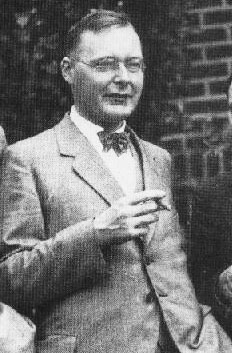
\includegraphics[]{complex/figures/h_kramers}
  \caption{Hans Kramers (1894–1952)}
\end{marginfigure}

The integral over the large semi--circle vanishes because of the big limit theorem. For the contribution of the small semi--circle around the pole $x_0$ we could use the small limit theorem, or alternatively calculate it directly:

\begin{align}
\lim_{\epsilon \to 0} & \int_{- \infty}^{x_0-\epsilon} \frac{f(x)}{x-x_0}dx + \nonumber \\
\lim_{\epsilon \to 0} & \int_{\pi}^0 \frac{f(x_0+\epsilon e^{j \theta})}{\epsilon e^{j\theta}} \epsilon j e^{j \theta} d \theta + \nonumber \\
\lim_{\epsilon \to 0} & \int_{x_0+\epsilon}^{\infty} \frac{f(x)}{x-x_0}dx = 0
\end{align} 

This leads to 

\begin{equation}
f(x_0) = \frac{1}{\pi j} PV \int_{- \infty}^{\infty} \frac{f(x)}{x-x_0}dx
\label{eq-kk-1}
\end{equation} 

If you squint a bit, you could say that the singularity $x_0$ lies more or less on our contour (although we avoided it with the small semicircle). You could therefore say that it's halfway between a singularity outside of the contour (Cauchy's theorem) and one inside the contour (Cauchy's formula). This is also reflected in the result of the integral, which is the average of these two cases, with an extra principal value thrown in for good measure.

\begin{exer}
  % difficulty: trivial
  % youtube: lSqZlxCTX-s
Show that Eq.~\ref{eq-kk-1} can also be obtained by choosing a contour that circles around $x_0$ in the lower half of the complex plane.
\end{exer}

\begin{cue}
Split up Eq.~\ref{eq-kk-1} into its real and imaginary parts to derive expressions for $ u(x_0)= \Re f(x_0)$ and $ v(x_0)= \Im f(x_0)$.
\end{cue}

\begin{marginfigure}[-1.5cm]
  % credits: Wikipedia
  % url: https://en.wikipedia.org/wiki/Ralph_Kronig
  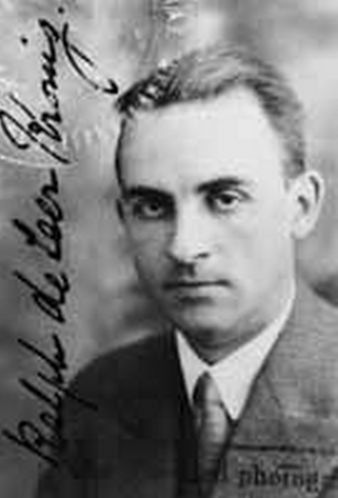
\includegraphics{complex/figures/r_kronig}
  \caption{Ralf Kronig (1904–1995)}
\end{marginfigure}

Splitting Eq.~\ref{eq-kk-1} into real and imaginary parts yields

\begin{align}
f(x_0) =& \, u(x_0) + jv(x_0) \nonumber \\
       =& \, \frac{1}{\pi j} PV \int_{- \infty}^{\infty} \frac{u(x)+jv(x)}{x-x_0}dx
 \nonumber \\
       =& \, \frac{1}{\pi} PV \int_{- \infty}^{\infty} \frac{v(x)}{x-x_0}dx -
\frac{j}{\pi} PV \int_{- \infty}^{\infty} \frac{u(x)}{x-x_0}dx
\end{align}

or

\begin{subequations} 
\begin{equation}
u(x_0) = \frac{1}{\pi} PV \int_{- \infty}^{\infty} \frac{v(x)}{x-x_0}dx
\end{equation} 
\begin{equation}
v(x_0) = -\frac{1}{\pi} PV \int_{- \infty}^{\infty} \frac{u(x)}{x-x_0}dx
\end{equation}
\label{eq-KK}
\end{subequations}

\begin{marginfigure}[-1.5cm]
  % credits: Wikipedia
  % url: https://en.wikipedia.org/wiki/David_Hilbert
  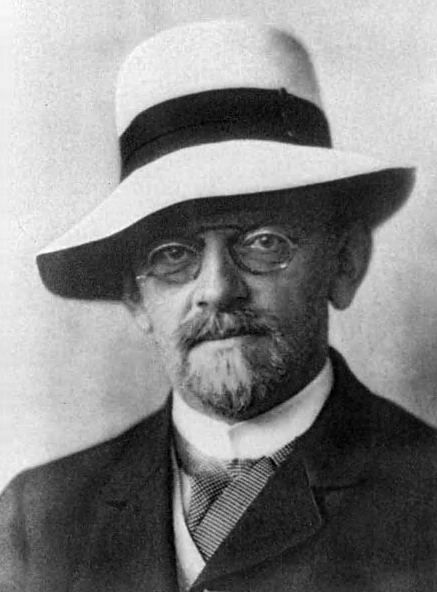
\includegraphics{complex/figures/d_hilbert}
  \caption{David Hilbert (1862–1943)}
\end{marginfigure}

Equations \ref{eq-KK} are called the \emph{Kramers--Kronig} dispersion relations. They state that under the conditions given above, the real part of a function can be expressed as an integral over the imaginary part and vice--versa.

By definition, equations \ref{eq-KK} also express that the real and imaginary parts are \emph{Hilbert transforms} of each other. Hilbert transforms also find use in e.g. telecommunications.

Let's now apply this to the field of material dispersion by applying these relations to the function $f(z) = \chi(\omega) =
n(\omega)^2 -1$. $\chi(\omega)$ is a material's susceptibility and relates the polarisation $\mathbf{P}$ to the incident electric field $\mathbf{E}$ according to $\mathbf{P}(\omega)=\varepsilon_0 \chi(\omega) \mathbf{E}(\omega)$).

\begin{exer}
  % difficulty: normal
  % youtube: e5txdhhmaKI
What is the mathematical reason we used $f(z) = \chi(\omega)$ here, and not e.g. $f(z) = n(\omega)$? Link this to the physics of the problem. 
\end{exer}

Replacing $x_0$ by $\omega$, and $x$ by $\omega'$, we get

\begin{subequations} 
\begin{equation}
\Re \chi(\omega) = \frac{1}{\pi} PV \int_{- \infty}^{\infty} \frac{\Im
\chi(\omega')}{\omega'-\omega}d\omega'
\end{equation} 
\begin{equation}
\Im \chi(\omega) = -\frac{1}{\pi} PV \int_{- \infty}^{\infty} \frac{\Re
\chi(\omega')}{\omega'-\omega}d\omega'
\end{equation}
\label{eq-KK-2}
\end{subequations}

As you might remember, the imaginary part of the refractive index $n$ is a measure for optical absorption. So, this means e.g. that in theory it is enough to measure the losses of a material over a wide wavelength range to calculate its refractive index.

\begin{exer}
  % difficulty: normal
  % youtube: 4p0u-OYVqz8
Suppose you have a material without dispersion, i.e. where the real part of the squared refractive index is constant. Show that such a material is lossless, i.e. the imaginary part of the squared refractive index is zero.
\end{exer}

\begin{exer}
  % difficulty: trivial
  % youtube: RpV0_aDx9Gk
From basic logic and the result above, conclude that as soon as you have loss in a material, the material is necessarily dispersive. Also, convince yourself that the only non-dispersive material is vacuum.
\end{exer}

Recall the definition of the susceptibility in the time domain:

\begin{equation}
\mathbf{P}(t)=\varepsilon_0 \int_{-\infty}^t \chi(t-t') \mathbf{E}(t')\, dt'.
\end{equation}

From this, we can easily see that $\chi(t)$ is necessarily real, as complex numbers only show up in the frequency domain after the introduction of phasors. From this, one can derive that for its Fourier transform $\chi(-\omega) = \chi^*(\omega)$, which in turn has some implications on the even and odd character of the real and the imaginary parts of $\chi(\omega)$. These can be used to reformulate the Kramers--Kronig relations in another common form:

\begin{exer}
  % difficulty: hard
  % youtube: Goi6ApUWzbQ 
Given that $\chi(t)$ is real-valued, show that the Kramers--Kronig dispersion relations reduce to
$$\Re \chi(\omega) =  \frac{2}{\pi} PV \int_{0}^{\infty}{ \frac{\omega'\Im \chi(\omega')}{\omega'^2-\omega^2}d\omega'}$$
$$\Im \chi(\omega) = -\frac{2}{\pi} PV \int_{0}^{\infty}{ \frac{\omega \Re \chi(\omega')}{\omega'^2-\omega^2}d\omega'}$$

  \begin{hnt}
    Figure out whether $u(\omega)$ and $v(\omega)$ are even or odd, and split up the integral in contributions for positive and negative frequencies.
  \end{hnt}
\end{exer}

Finally, it's important to note that one can prove that there is a relation between the Kramers--Kronig dispersion relations and the fact that the systems considered are \emph{causal} (i.e. effect cannot precede cause)\noindent\marginnote{This is one of the subjects of the Titchmarsh theorem.}. Thus, there is an immediate physical significance of the Kramers--Kronig dispersion relations.


\pagebreak


\sectionugent{Conformal transformations}
\label{week3}

\subsection*{Angle--preserving transformations}

\begin{marginfigure}
\centering
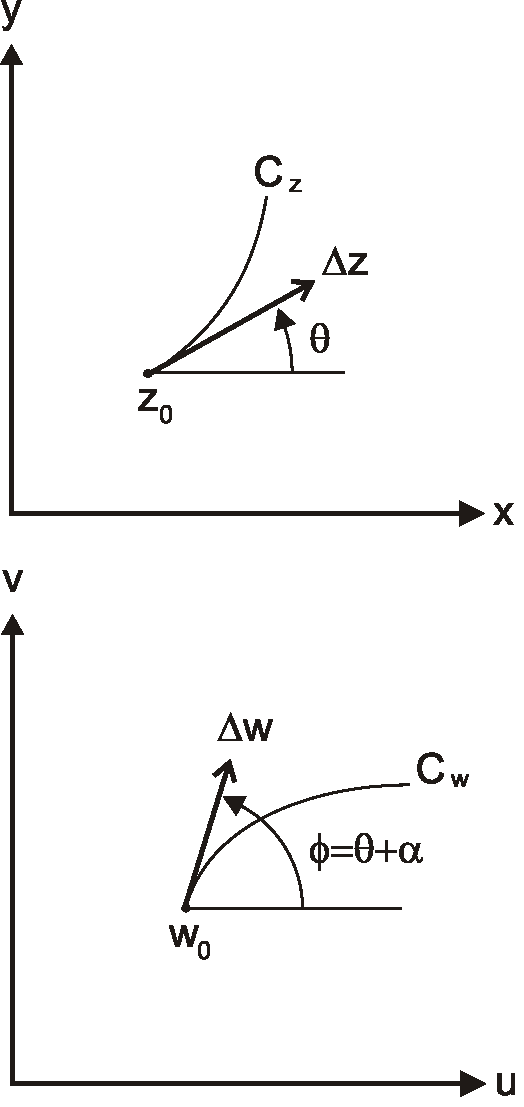
\includegraphics{complex/figures/conformal_portrait}
\caption{Conformal transformation.}
\label{fig-conformal}
\end{marginfigure}

A complex function $w = f(z) = u(x,y)+jv(x,y)$ can be seen as a mapping from the complex $z$--plane to the complex $w$--plane. One way to visualise this is to plot how a curve $C_z$ in the $z$--plane is transformed to a curve $C_w$ in the $w$--plane (see Fig.~\ref{fig-conformal}).

We can play this transformation game using two specific neighbouring points on $C_z$, e.g. $z_0$ and $z_0+\Delta z$. They get transformed to two neighbouring points on $C_w$, which we'll call imaginatively $w_0$ and $w_0+\Delta w$. In the limit of $\Delta z \to 0$, this will allow us to say something about the relationship between the tangents at the points $z_0$ and $w_0$.

\begin{cue}
Relate $\frac{df}{dz}$ to $\Delta z$ and $\Delta w$. Then look at the angles of the resulting expression to determine how the tangents rotate.
\end{cue}

As long as $w=f(z)$ is an analytic function, we have

\begin{equation}
\frac{df}{dz} = \frac{dw}{dz} = \lim_{\Delta z \to 0} \frac{\Delta w}{\Delta z}
\end{equation}

By putting this expression in polar form and looking at the angle, we can derive an expression relating the angles of the tangents at $z_0$ and $w_0$:

\begin{equation}
\arg \frac{df}{dz} = \arg \lim_{\Delta z \to 0} \frac{\Delta w}{\Delta z} = \arg
\lim_{\Delta z   \to 0} \Delta w - \arg \lim_{\Delta z \to 0} \Delta z
\end{equation} 

For an analytic function $\arg df / dz = \alpha$ (the angle of the derivative) depends on $z$, but for a given $z$ it is independent of the direction of approach. So, if in Fig.~\ref{fig-conformal} the angle of the increment $\Delta z$ with respect to the $x$--axis is $\theta$, and the increment $\Delta w$ forms an angle $\phi$ with the $u$ axis, we can relate these angles by

\begin{equation}
\phi = \theta + \alpha
\end{equation}

This also means that an analytic transformation will rotate any line in the $z$--plane over an angle of $\alpha$ in the $w$--plane. Since this result holds for any line through $z_0$, it obviously also holds for any \emph{pair} of lines. This means that for the angle between these two lines we get

\begin{equation}
\phi_2 - \phi_1 = (\theta_2 + \alpha) - (\theta_1 + \alpha) = \theta_2 -
\theta_1
\end{equation} 

From this we can see that such a transformation preserves the angle between any pair of lines. If such an angle--preserving transformation defined by an analytic function is also injective between two domains, it is called a \emph{conformal transformation}.

\subsection*{Conformal transformations and the Helmholtz equation}

Conformal transformations can be useful to solve the Helmholtz equation in a 'difficult' coordinate system. The idea is to use a conformal mapping to transform the coordinate system to a different one where the solution is more tractable. In this section, we will investigate what form the Helmholtz equation takes in the new domain.

Suppose our old $(x,y)$--coordinate system is related to a new $(u,v)$--coordinate system by a conformal transformation $f$:

\begin{equation}
u+jv = w = f(z) = f(x+jy)
\end{equation} 

In the $z$--plane, the Helmholtz equation in media with piecewise constant refractive index has the following form:

\begin{equation}
\frac{\partial^2 \psi(x,y)}{\partial x^2} + \frac{\partial^2 \psi(x,y)}{\partial y^2} + k_0^2 n^2(x,y) \psi(x,y) = 0
\end{equation}

\begin{cue}
Use the chain rule to express $\frac{\partial \psi}{\partial x}$ using partial derivatives with respect to $u$ and $v$.
\end{cue}

Application of the chain rule leads to

\begin{equation}
\frac{\partial \psi}{\partial x} = \frac{\partial \psi}{\partial u}
\frac{\partial u}{\partial x} + \frac{\partial \psi}{\partial v} \frac{\partial
v}{\partial x}
\end{equation} 

\begin{cue}
Now calculate $\frac{\partial^2 \psi}{\partial x^2}$.
\end{cue}

For the second derivative this becomes

\begin{equation}
\frac{\partial^2 \psi}{\partial x^2} = \frac{\partial}{\partial x} \left[
\frac{\partial \psi}{\partial u}\right]  \frac{\partial u}{\partial x} +
\frac{\partial \psi}{\partial u}\frac{\partial^2 u}{\partial x^2} +  
\frac{\partial}{\partial x} \left[ \frac{\partial \psi}{\partial v}\right] 
\frac{\partial v}{\partial x}  + \frac{\partial \psi}{\partial
v}\frac{\partial^2 v}{\partial x^2}
\end{equation} 

Or

\begin{align}
\frac{\partial^2 \psi}{\partial x^2} = &\left[ \frac{\partial^2 \psi}{\partial u^2 } \frac{\partial u}{\partial x} +  \frac{\partial^2 \psi}{\partial u \partial v} \frac{\partial v}{\partial x} \right] \frac{\partial u}{\partial x}  + \frac{\partial \psi}{\partial u}\frac{\partial^2 u}{\partial x^2} \nonumber \\ 
+ &\left[ \frac{\partial^2 \psi}{\partial v^2 } \frac{\partial v}{\partial x} + 
\frac{\partial^2 \psi}{\partial u \partial v} \frac{\partial u}{\partial x}
\right] \frac{\partial v}{\partial x} + \frac{\partial \psi}{\partial v}\frac{\partial^2 v}{\partial x^2}
\end{align} 

\begin{cue}
Now add these two second-order derivatives and go on a term-cancelling spree. Remember that the Cauchy-Riemann conditions hold. Also, note that for a holomorphic function $\nabla^2 u = \nabla^2 v=0$.
\end{cue}

For the total Laplacian we get

\begin{align}
\frac{\partial^2 \psi}{\partial x^2} &+ \frac{\partial^2 \psi}{\partial y^2}= \nonumber \\
  &\frac{\partial^2 \psi}{\partial u^2 }  \left [ \left(\frac{\partial u}{\partial x}\right)^2 + \left(\frac{\partial u}{\partial y}\right)^2\right]+ \frac{\partial \psi}{\partial u} \left[ \frac{\partial^2 u}{\partial x^2}  + \frac{\partial^2 u}{\partial y^2} \right] + 2\frac{\partial^2 \psi}{\partial u \partial v} \frac{\partial u}{\partial x} \frac{\partial v}{\partial x}    \nonumber \\  
+ &\frac{\partial^2 \psi}{\partial v^2}  \left[ \left(\frac{\partial v}{\partial
x}\right)^2 + \left(\frac{\partial v}{\partial y}\right)^2\right] + \frac{\partial
\psi}{\partial v} \left[ \frac{\partial^2 v}{\partial x^2} + \frac{\partial^2 v}{\partial y^2} \right] + 2\frac{\partial^2 \psi}{\partial u \partial v} \frac{\partial u}{\partial y} \frac{\partial v}{\partial y}
\label{eq-conf-trans-1}
\end{align} 

It is easy to see that terms three and six cancel because of the Cauchy--Riemann conditions.

We know from Ex.~\ref{ex-harmonic} that for a holomorphic function $\nabla^2 u =
\nabla^2 v=0$, so the second and the fifth term on the right--hand--side of
Eq.~\ref{eq-conf-trans-1} vanish as well.

\begin{cue}
What does Cauchy--Riemann teach us about the factors in square brackets in terms one and four?
\end{cue}

Because of the Cauchy--Riemann equations, we can write

\begin{equation}
\left(\frac{\partial u}{\partial x}\right)^2 + \left(\frac{\partial u}{\partial
y}\right)^2 = \left(\frac{\partial v}{\partial x}\right)^2  +
\left(\frac{\partial v}{\partial y}\right)^2 = 
\left(\frac{\partial u}{\partial x}\right)^2 + \left(\frac{\partial v}{\partial
x}\right)^2 
 \stackrel{def}{=} \frac{1}{T(u,v)^2} \label{eq-T-factor}
\end{equation} 

So finally, we can write the Helmholtz equation in the transformed domain as

\begin{equation}
\frac{\partial^2 \psi(u,v)}{\partial u^2} + \frac{\partial^2 \psi(u,v)}{\partial
v^2} + k_0^2 T^2(u,v)n^2(u,v) \psi(u,v) = 0
\end{equation} 

Formally, this is identical to the Helmholtz equation in the $z$--plane, except that \emph{the index distribution $n$ has been replaced by a transformed index distribution $T \cdot n$}.

\subsection*{Application: bent waveguides}

\begin{marginfigure}[-6cm]
\centering
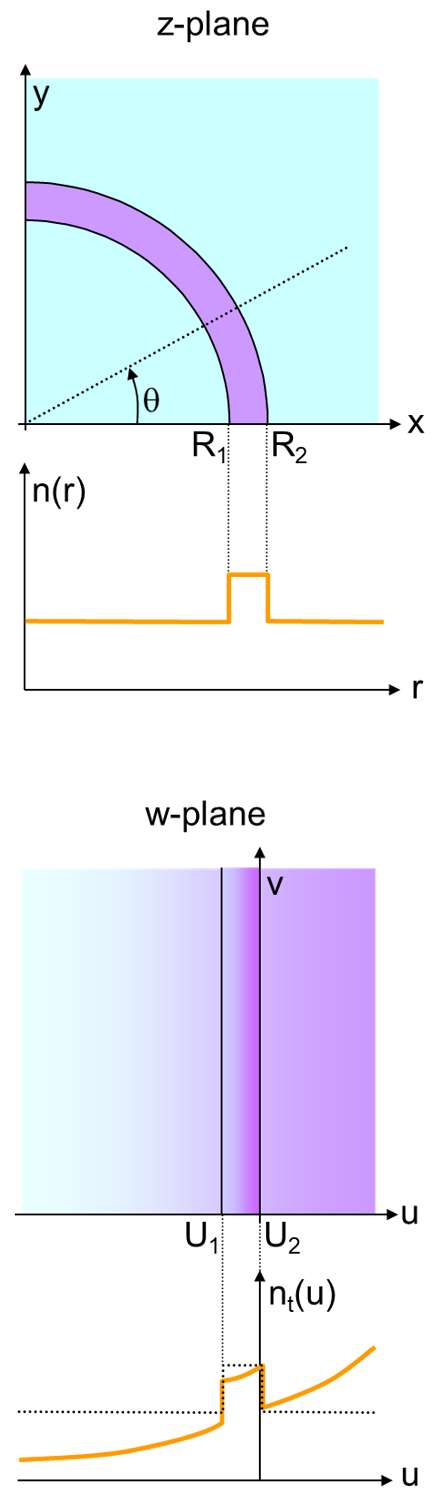
\includegraphics{complex/figures/bends_portrait}
\caption{Calculating bend modes using conformal transformation.}
\label{fig-bends}
\end{marginfigure}

To give an example of the power of conformal transformations, we will use it to find the eigenmodes of a bent dielectric waveguide (Fig.~\ref{fig-bends}). We consider the system to be invariant in the $z$--direction.

To tackle this problem, we could formulate the Helmholtz equation in cylindrical
coordinates, and the solution would involve Bessel functions. Here however, we will use the following conformal transformation to convert the curved geometry to a straight one:

\begin{equation}
w = R_2 \ln \frac{z}{R_2}
\end{equation} 

\begin{cue}
Transform this to polar coordinates and verify that this indeed straightens the bend.  
\end{cue}

With $z=r e^{j \theta}$, we can write this as

\begin{equation}
u + jv = R_2 \ln \frac{r}{R_2} + j R_2 \theta
\end{equation} 

This clearly shows the effect of the transformation: a circular path in the $z$--plane with constant $r$ is transformed to a straight path in the $w$--plane with constant $u$ (see Fig.~\ref{fig-bends}).

\begin{cue}
Calculate the transformation factor $T$. 
\end{cue}

Using the definition of the transformation factor $T$ from Eq.~\ref{eq-T-factor}, we get

\begin{equation}
\frac{\partial u}{\partial x} = \frac{R_2}{r}\frac{\partial r}{\partial x} = 
\frac{R_2}{\sqrt{x^2+y^2}} \cdot \frac{2x}{2\sqrt{x^2+y^2}} = R_2
\frac{x}{x^2+y^2}
\end{equation} 

Also,

\begin{equation}
\frac{\partial v}{\partial x} = R_2 \frac{\partial}{\partial x} \arctan
\frac{y}{x} = \frac{R_2}{1 + \frac{y^2}{x^2}} \cdot y \cdot \frac{-1}{x^2}= -R_2
\frac{y}{x^2+y^2}
\end{equation} 

So finally

\begin{equation}
T = \frac{1}{\sqrt{u_x^2+v_x^2}} = \frac{\sqrt{x^2+y^2}}{R_2} =
\frac{r}{R_2}=e^{\frac{u}{R_2}}
\end{equation} 

In the new coordinate system, the transformed index profile looks like

\begin{equation}
n_t(u) = n(u)e^{\frac{u}{R_2}}
\end{equation} 

This profile is sketched in Fig.~\ref{fig-bends}. The rest of the solution now proceeds as follows. The continuous index profile is approximated by a stepwise constant profile with a large number of steps. The modes of such a waveguide can be readily found by using standard techniques.

When this way of calculating the modes of a bent waveguide was first proposed in the 1970s, the calculation power of computers was nothing to write home about, so any trick that could simplify a problem was very welcome. Today, the interest of these techniques is more instructional than practical, although it does allow us to get some physical insight.

\begin{cue}
Making use of the tendency of light to concentrate in regions with high refractive index, think about how light in these bent waveguides will behave. What happens if the radius of curvature decreases?  
\end{cue}

Because the refractive index is higher near the outside of the bend, the mode will tend to be concentrated there. There is also the opportunity for the light to tunnel towards the outer cladding, where the index is even higher. This is the origin of the radiation losses in waveguide bends. Tighter bends (i.e. shorter radii) will be more prone to this phenomenon, because the steeper exponential will reduce the tunneling distance.


\section*{Review questions}

\begin{itemize}
\item What is a holomorphic function?
\item What are the Cauchy-Riemann conditions?
\item What is Cauchy's theorem?
\item What is Cauchy's formula?
\item What is a Laurent series?
\item What type of poles can a function have?
\item What are branch points and branch cuts?
\item What is the Riemann surface?
\item What is a residue?
\item How do you calculate the residue of a single pole?
\item What is the residue theorem?
\item What is Jordan's lemma?
\item What are the big and small limit theorems?
\item What is the principal value of an integral?
\item How do you solve integrals of the type $\int_0^{2 \pi} f(\cos \theta, \sin \theta) d \theta$?
\item How do you solve integrals of the type  $\int_\infty^{\infty} f(z) e^{jbz} dz$?
\item What do the Kramers-Kronig relations express?
\item What are conformal transformations and what are they used for?
\end{itemize}

%%% Local Variables:
%%% mode: latex
%%% TeX-master: "../main"
%%% End:

\chapter{Special functions}
\label{h:special}

\begin{quote}
We must admit with humility that, while number is purely a product of our minds, space has a reality outside our minds, so that we cannot completely prescribe its properties a priori.

-- Carl Friedrich Gauss, letter to Bessel
\end{quote}

\begin{quote}
We are servants rather than masters in mathematics.

--- Charles Hermite
\end{quote}

\etocsetstyle{section}
{}
{\leavevmode\leftskip 0cm\relax}
{\bfseries\normalsize\makebox[1.cm][l]{\etocnumber}%
\etocname\nobreak\hfill\nobreak
\rlap{\makebox[0.5cm]{\etocpage\mdseries}}\par}
{}

\etocsetstyle{section}
{}
{\leavevmode\leftskip 0.2cm \rightskip 0.6cm  \relax}
{\makebox[1.cm][l]{\etocnumber}%
\etocname\nobreak\dotfill\nobreak
\rlap{\makebox[0.7cm][r]{\etocpage}}\par\vspace{-2mm}}
{}

\etocsettocdepth{1}

%\etocsettocstyle{{\bfseries{\textcolor{headingbordeaux}{{\large %Contents}}}}\\\rule{\textwidth}{0.4pt}\\\begin{small}}%
%  {\end{small}\rule{\textwidth}{0.4pt}}

\etocsettocstyle{}{}

\bigskip
\bfseries
\textcolor{headingbordeaux}{\large Contents}
\vspace{-5mm}

\rule{\textwidth}{0.4pt}
\vspace{-7mm}
\begin{small}
\localtableofcontents
\end{small}
\mdseries
\vspace{-3mm}
\rule{\textwidth}{0.4pt}
\smallskip

In this chapter, we will look at two different classes of 'special' functions. The first class consists of Bessel functions and their cousins the Neumann and the Hankel functions. These naturally occur when solving problems in cylindrical coordinate systems. The second class of functions are the Hermite polynomials. These are an example of a family of so-called orthogonal polynomials. They appear in the higher-order solutions of the paraxial wave equation.

For both classes, we will follow a similar structure. After presenting their corresponding differential equations, we introduce a different way of defining these functions based on so-called generating functions. These are useful to more easily prove all sorts of useful properties, like recurrence relationships. Additionally, we will tackle integrals involving the special functions, derive their orthogonality, as well as use them in series expansions.


\pagebreak


\sectionugent{Bessel's differential equation}\label{sec-bessel-eq}

Writing the Helmholtz equation Eq.~\ref{eq-helmholtz} in cylindrical coordinates gives us

\begin{equation}
\frac{\partial^2 \psi}{\partial r^2} + \frac{1}{r} \frac{\partial \psi}{\partial r} +\frac{1}{r^2} \frac{\partial^2 \psi}{\partial \theta^2} + \frac{\partial^2 \psi}{\partial z^2} + k_0^2 n^2\psi = 0 \label{eq-helmholtz-cyl}
\end{equation}

Here, $\psi$ can represent any of the Cartesian components of the electric or magnetic field, or the axial coordinates $E_z$ and $H_z$ in cylindrical coordinates.

We assume that we are looking at a region of space where $n$ is constant. Let's try a solution of the following form, with $k_\theta$ and $k_z$ constant: 

\begin{equation}
\psi(r,\theta,z) = R(r)e^{-j k_\theta \theta }e^{-j k_z z}
\label{eq-bessel-ansatz}
\end{equation}  

Later in this chapter, we will deal with the physical interpretation behind this expression.

\begin{cue}
Substitute Eq.~\ref{eq-bessel-ansatz} in Eq.~\ref{eq-helmholtz-cyl}.
\end{cue}

This leads to

\begin{equation}
\frac{d^2 R(r)}{d r^2} + \frac{1}{r} \frac{d R(r)}{d r} + \left[k_0^2 n^2 - k_z^2 - \frac{k_\theta^2}{r^2} \right] R(r) = 0
\end{equation} 

Or

\begin{equation}
r^2\frac{d^2 R(r)}{d r^2} + r \frac{d R(r)}{d r} + \left[ r^2 (k_0^2 n^2 - k_z^2)- k_\theta^2 \right] R(r) = 0
\end{equation}

Let's make this a little bit more generic, without explicit references to the wave equation.

For that, we can renaming $R$ to $X$ and $k_\theta$ to $\nu$, as well as make the following change of variables

\begin{equation}
x = r \sqrt{k_0^2 n^2 - k_z^2} \stackrel{def}{=} k_t r
\end{equation}

\begin{cue}
  Implement those changes.
\end{cue}

This leads to

\begin{equation}
\fbox{$\displaystyle
x^2\frac{d^2 X(x)}{d x^2} + x \frac{d X(x)}{d x} + \left(x ^ 2 - \nu^2 \right)X(x) = 0 \label{eq-bessel}
$}
\end{equation}

Eq.~\ref{eq-bessel} is called Bessel's differential equation. A solution to this equation is given by $J_\nu(x)$, the Bessel function of the first kind of order $\nu$.

In what follows, we will mostly consider the important special case where $\nu$ is an integer. In this situation, we will use the notation $J_n(x)$, where $n$ is the integer version of $\nu$ and is not to be confused with the refractive index $n$ in Eq.~\ref{eq-helmholtz-cyl}.

\sectionugent{Generating function for Bessel functions}

One way of figuring out what these Bessel functions look like, would be to propose a Taylor series expansion, substitute that into the differential equation, and then derive the expansion coefficients. However, here we'll take a completely different approach to define Bessel functions (at least for integer order). Later on, we'll show that this new approach is equivalent to the original differential equation.

\noindent\marginnote{This is a purely mathematical trick. $t$ does not represent time, and in fact has no physical meaning at all.}Let's introduce a function of two variables, a so-called \emph{generating function}:

\begin{equation}
g(x,t) \stackrel{def}{=} e^{x/2(t-1/t)} \label{eq-gen-bessel}
\end{equation}

When we expand this function in a Laurent series in $t$, we \emph{define} the coefficients as being the Bessel functions:

\begin{equation}
e^{x/2(t-1/t)}  \stackrel{def}{=} \sum_{n = - \infty}^{\infty} J_n(x)t^n \label{eq-g-bessel}
\end{equation}

\begin{cue}
By expanding the exponentials in the equation above, derive a series expansion for  $J_n(x)$.  
\end{cue}

Expanding the exponentials in Eq.~\ref{eq-g-bessel} gives us

\begin{equation}
e^{xt/2} \cdot e^{-x/2t} = \sum_{r = 0}^{\infty} {\left(\frac{x}{2}\right)}^r \frac{t^r}{r!} \cdot \sum_{s = 0}^{\infty} {(-1)}^s { \left(\frac{x}{2}\right)}^s \frac{t^{-s}}{s!}
\end{equation} 

Introducing a new variable $n = r - s$ and getting rid of $r$, we can reorganise this equation to give

\begin{equation}
e^{xt/2} \cdot e^{-x/2t} = \sum_{n = -\infty}^{\infty} \left[ \sum_{s = 0}^{\infty} {\left(\frac{x}{2}\right)}^{n+s} \frac{1}{(n+s)!} \cdot (-1)^s {\left(\frac{x}{2}\right)}^{s} \frac{1}{s!} \right] t^n
\end{equation} 

This means that

\begin{equation}
\fbox{$\displaystyle
J_n(x) = \sum_{s = 0}^{\infty} \frac {{(-1)}^s}{s!(n+s)!} {\left(\frac{x}{2}\right)}^{n+2s} \label{eq-bessel-series}
$}
\end{equation} 

This series expansion can be used to numerically calculate the Bessel functions. Fig.~\ref{fig-bessel-J} plots $J_0(x)$, $J_1(x)$, $J_2(x)$. These functions oscillate, but are not periodic.

\begin{figure}
\centering
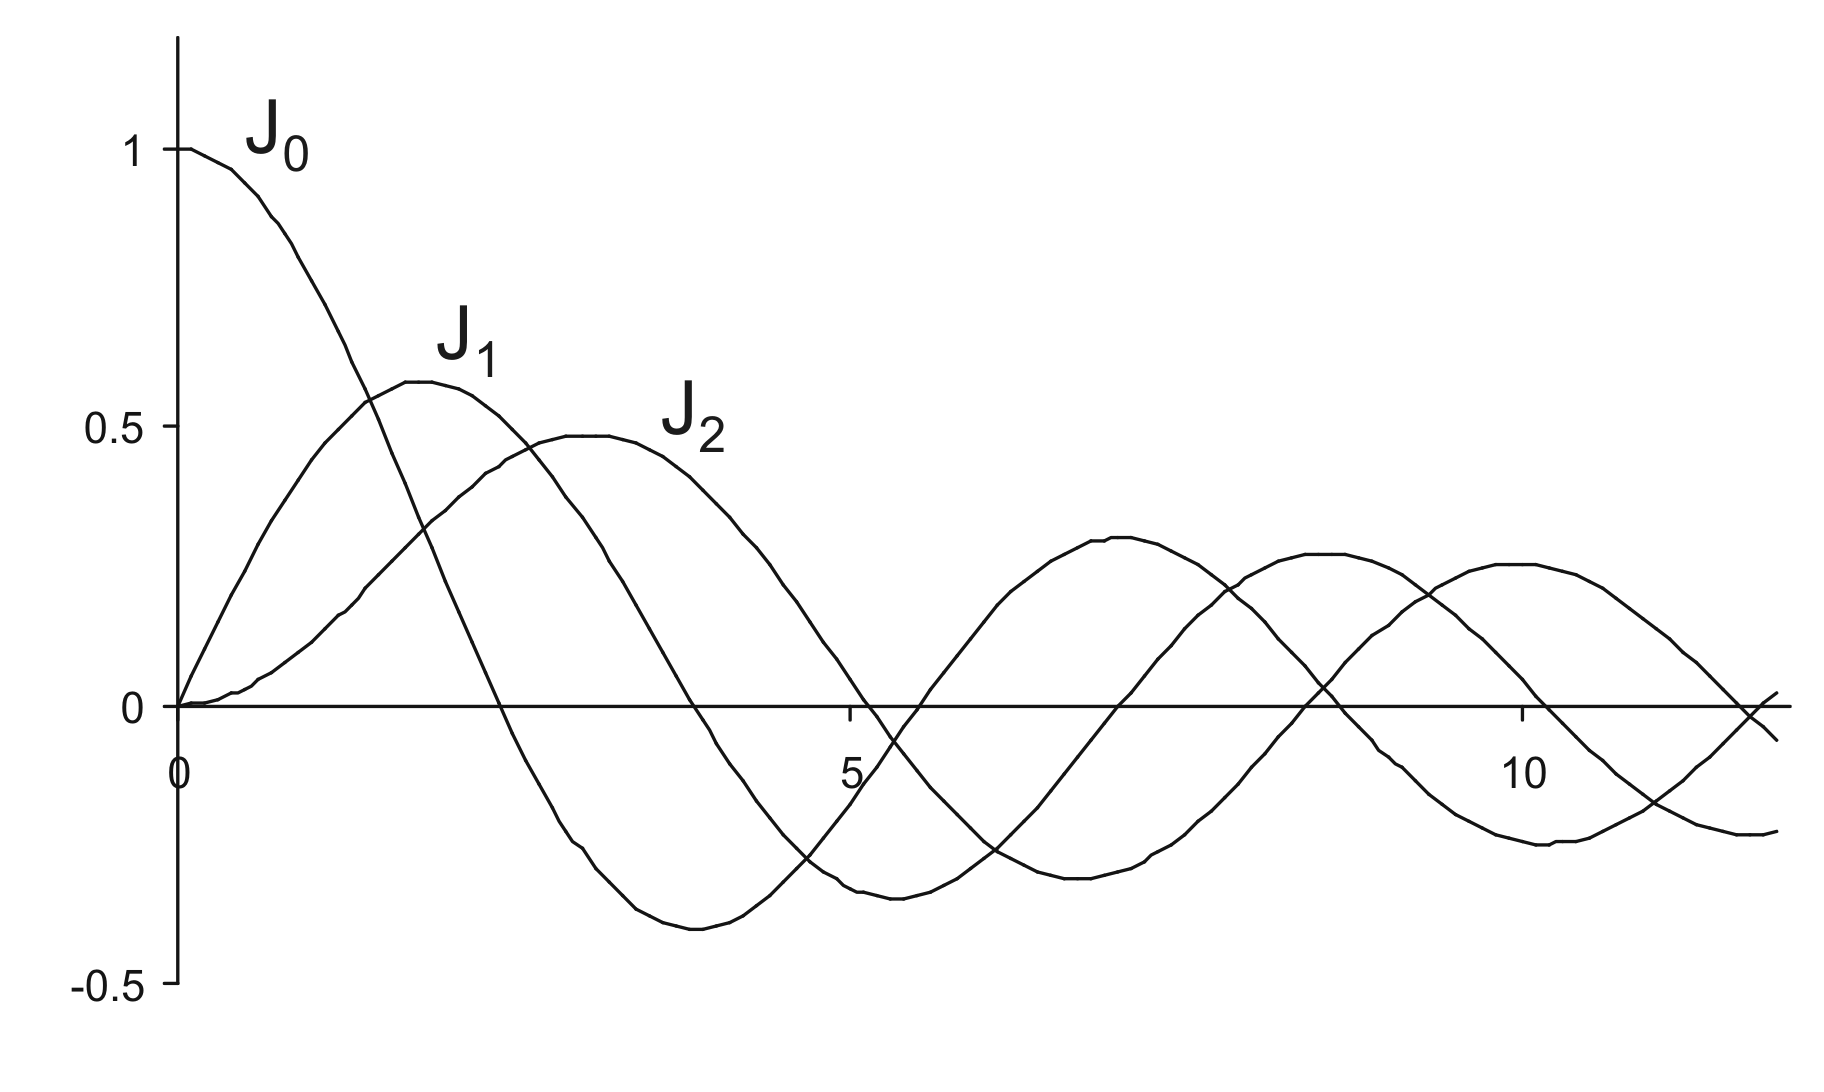
\includegraphics[scale=0.7]{special/figures/j}
\caption{The Bessel functions $J_0(x)$, $J_1(x)$ and $J_2(x)$.}
\label{fig-bessel-J}
\end{figure}

\begin{exer}
% difficulty: normal
Show that
$$\lim_{x \to 0} \frac{J_1(x)}{x}= \frac{1}{2}$$
\end{exer}

\begin{exer}
% difficulty: trivial
% ugent
Use the definition of the generating function Eq.~\ref{eq-g-bessel} to show that
$$J_{-n}(x)=(-1)^nJ _n(x)$$
Hint: try replacing $t$ by $-1/t$ in the generating function.
\end{exer}

\begin{exer}
% difficulty: normal
Use the product of the generating functions $g(x,t)$ and $g(x,-t)$ to show that
$$\left[ J_0(x) \right]^2 + 2 \sum_{n=1}^\infty \left[ J_n(x) \right]^2 = 1 $$
\end{exer}

\begin{sidebar}
\begin{ex}
By evaluating the generation function in a suitable point, prove the following
$$ \cos x =  J_0(x) + 2 \sum_{n=1}^\infty (-1)^n J_{2n}(x)  $$
$$ \sin x =  2 \sum_{n=0}^\infty (-1)^n J_{2n+1}(x)  $$
\end{ex}
\end{sidebar}

\begin{sidebar}
\begin{ex}
Evaluate the following contour integral along the unit circle in the complex $t$-plane:

$$ \oint_C t^{-n-1} g(x,t) dt $$

In doing so, derive the following equations:

$$J_n(x) = \frac {1}{2\pi} \int_0 ^ {2 \pi} \cos (n \theta - x \sin \theta ) d\theta $$

$$ J_0(x) =  \frac {1}{2\pi} \int_0 ^ {2 \pi}  e^{j x \cos \theta} d \theta $$
\end{ex}
\end{sidebar}


\sectionugent{Recurrence relations for Bessel functions}

If we differentiate Eq.~\ref{eq-g-bessel} with respect to $t$, we get

\begin{equation}
\frac{x}{2}\left({1 + \frac{1}{t^2}}\right) e^{x/2(t-1/t)} = \sum_{n = - \infty}^{\infty} n J_n(x)t^{n-1}
\end{equation}

Substituting Eq.~\ref{eq-g-bessel} back into this, we get

\begin{equation}
\frac{x}{2}\left({1 + \frac{1}{t^2}}\right) \sum_{n = - \infty}^{\infty} J_n(x)t^n = \sum_{n = - \infty}^{\infty} n J_n(x)t^{n-1}
\end{equation} 

Equating the coefficients of like powers of $t$ we get

\begin{equation}
\frac{x}{2} J_n(x) + \frac{x}{2} J_{n+2}(x) = (n+1)J_{n+1}(x)
\end{equation} 

Or with the substitution $n+1 \to n$

\begin{equation}
\fbox{$\displaystyle
J_{n-1}(x) + J_{n+1}(x) = \frac{2n}{x} J_n(x)
$}
\end{equation} 

\begin{sidebar}
\begin{ex}
Differentiate the generating function with respect to $x$ to show that
$$\fbox{$\displaystyle J_{n-1}(x) - J_{n+1}(x) = 2 J_n'(x)$}$$ \label{ex-recur}
\end{ex}
\end{sidebar}

\begin{sidebar}
\begin{ex}
Show that
$$\begin{array}{lcll}a) & J_{n-1}(x) = \frac{n}{x}J_n(x) + J_n'(x) \\b) & J_{n+1}(x) = \frac{n}{x}J_n(x) - J_n'(x) \\c) & \frac{d}{dx}\left[x^n J_n(x)\right] = x^n J_{n-1}(x) \\d) & \frac{d}{dx}\left[x^{-n} J_n(x)\right] = -x^{-n} J_{n+1}(x)\end{array}$$ \label{ex-recurrence}
\end{ex}
\end{sidebar}


\begin{sidebar}
\begin{ex}
First, show that
$$\int_0^\infty J_1( x) dx =  1$$
Then, extend this to show that
$$\int_0^\infty J_1( x) dx = \int_0^\infty J_3( x) dx = \int_0^\infty J_5( x) dx = \cdots = 1$$
\end{ex}
\end{sidebar}

\begin{sidebar}
\begin{ex}
Show that
$$\int_0^1 x^3 J_0(k x) dx =  \frac{J_1(k)}{k} - 2 \frac{J_2(k)}{k^2}$$
If $k$ is a zero of $J_0$, show that this integral is equal to
$$\frac{J_1(k)}{k^3}\left(k^2-4\right)$$
\end{ex}
\end{sidebar}

\begin{sidebar}
\begin{ex}
Fraunhofer diffraction is governed by the following equation:

$$U(x_0, y_0) \sim \iint_{-\infty}^{\infty} U(x_1, y_1) e ^{j \frac{2\pi}{\lambda z} (x_0 x_1 + y_0 y_1)} dx_1 dy_1  $$

By using polar coordinates both in the aperture plane

$$x_1 = \rho_1 \cos \theta_1; \quad y_1 = \rho_1 \sin \theta_1$$

and the observation plane

$$x_0 = \rho_0 \cos \theta_0; \quad y_0 = \rho_0 \sin \theta_0$$

show that for rotationally symmetric apertures this reduces to

$$U(\rho_0) \sim  \int_0^{\infty} \int_0^{2 \pi} U(\rho_1)  e ^{j \frac{2\pi}{\lambda z} \rho_0 \rho_1 \cos \theta_1} \rho_1 d\rho_1 d\theta_1  $$

Then, proceed to calculate the so-called Airy diffraction pattern for a circular aperture of radius $a$:

$$U(\rho_0) \sim \frac {J_1\left( 2 \pi \frac {\rho_0 a}{\lambda z} \right)}{\frac{\rho_0}{\lambda z a}}$$

\end{ex}
\end{sidebar}

\section{Bessel's differential equation revisited}

From Ex. \ref{ex-recurrence}, we get

\begin{equation}
J_{n-1}(x) = \frac{n}{x}J_n(x) + J_n'(x)
\end{equation}

This can be written as

\begin{equation}
x J_n'(x) + n J_n(x) - x J_{n-1}(x) = 0 \label{eq-bessel-dif-rec}
\end{equation} 

Differentiating with respect to $x$, we get

\begin{equation}
J_n'(x) + x J_n''(x) + n J_n'(x) - J_{n-1}(x) - x J_{n-1}'(x)= 0
\end{equation} 

or after multiplying by $x$:

\begin{equation}
x^2 J_n''(x) + (n + 1) x J_n'(x) - x J_{n-1}(x) - x^2 J_{n-1}'(x)= 0
\end{equation} 

We now subtract Eq.~\ref{eq-bessel-dif-rec} multiplied by $n$:

\begin{equation}
x^2 J_n''(x) + (n + 1) x J_n'(x) - x J_{n-1}(x) - x^2 J_{n-1}'(x) - n\left(x J_n'(x) + n J_n(x) - x J_{n-1}(x)\right)= 0
\end{equation} 

This simplifies to

\begin{equation}
x^2 J_n''(x) +  x J_n'(x) - x^2 J_{n-1}'(x) - n^2 J_n(x) + (n - 1) x J_{n-1}(x)= 0 \label{eq-bessel-dif-rec-2}
\end{equation} 

As a next step, we now take another recurrence equation from Ex. \ref{ex-recurrence}:

\begin{equation}
J_{n+1}(x) = \frac{n}{x}J_n(x) - J_n'(x)
\end{equation} 

Replacing $n$ with $n-1$, this can be written as

\begin{equation}
x J_{n}(x) = (n-1)J_{n-1}(x) - x J_{n-1}'(x)
\end{equation} 

With this, we can eliminate $J_{n-1}$ and $J_{n-1}'$ from Eq.~\ref{eq-bessel-dif-rec-2}:

\begin{equation}
x^2 J_n''(x) +  x J_n'(x) + x^2 J_n(x) - n^2 J_n(x) = 0
\end{equation} 

This is nothing other than Bessel's differential equation Eq.~\ref{eq-bessel}.

This shows that any function satisfying the recurrence relations used (also for non--integer values of $n$), also satisfies Bessel's equation. This is true in particular for the functions defined through our generating function Eq.~\ref{eq-gen-bessel}.

\sectionugent{Fourier--Bessel series}

Bessel functions can be used as a basis set for a series expansion of an arbitrary function. Before we can tackle this, we require some orthogonality relations for which we need to calculate a certain type of integral.

\subsection*{Lommel's integral}

Consider the following two differential equations:

\begin{equation}
x^2 \frac{d^2 \phi}{dx^2}  + x \frac{d \phi}{dx} + \left(l^2x^2 - n^2\right) \phi = 0 \label{eq-bessel-orth-1}
\end{equation} 

\begin{equation}
x^2 \frac{d^2 \psi}{dx^2}  + x \frac{d \psi}{dx} + \left(k^2x^2 - n^2\right) \psi = 0 \label{eq-bessel-orth-2}
\end{equation} 

Solutions to these equations are $J_n(lx)$ and $J_n(kx)$ respectively. By multiplying Eq.~\ref{eq-bessel-orth-1} with $\psi/x$, Eq.~\ref{eq-bessel-orth-2} with $\phi/x$ and subtracting the two results, we get

\begin{equation}
x \left( \frac{d^2 \phi}{dx^2}\psi - \frac{d^2 \psi}{dx^2} \phi \right) + \left(\psi \frac{d \phi}{dx}- \frac{d \psi}{dx}\phi\right) + \left(l^2 - k^2\right) x \phi \psi = 0
\end{equation}

This can be written as

\begin{equation}
\frac{d}{dx}\left[x \left( \frac{d \phi}{dx} \psi - \frac{d \psi}{dx} \phi\right)\right] = \left(k^2 - l^2\right) x \phi \psi
\end{equation}

such that

\begin{equation}
x \left[{\frac{dJ_n(lx)}{dx}  J_n(kx) - \frac{dJ_n(kx)}{dx} J_n(lx)}\right] + C = \left(k^2 - l^2\right)\int x J_n(lx)J_n(kx)dx
\end{equation}

With prime denoting derivation with respect to the \emph{entire} argument, we have $dJ_n(kx)/dx = kJ_n'(kx)$ and $dJ_n(lx)/dx = lJ_n'(lx)$, such that for $l \ne \pm k$

\begin{equation}
\int x J_n(lx)J_n(kx)dx = \frac{x}{k^2 - l^2} \left[{l J_n'(lx) J_n(kx) -  k J_n'(kx) J_n(lx)}\right] + C \label{eq-lommel-1}
\end{equation} 

The second recurrence relation from Ex. \ref{ex-recurrence} takes the form

\begin{equation}
J_n'(lx) =  \frac{n}{lx}J_n(lx)-J_{n+1}(lx)
\end{equation} 

Likewise,
\begin{equation}
J_n'(kx) =  \frac{n}{kx}J_n(kx)-J_{n+1}(kx)
\end{equation} 

So, Eq.~\ref{eq-lommel-1} becomes

\begin{equation}
\int x J_n(lx)J_n(kx)dx = \frac{x}{k^2 - l^2} \left[{k J_{n+1}(kx) J_n(lx) - l J_{n+1}(lx) J_n(kx)}\right] + C \label{eq-lommel-2}
\end{equation} 

Eq.~\ref{eq-lommel-2} is called Lommel's integral.

\subsection*{Orthogonality of Bessel functions}

Suppose that $\xi_i$ and $\xi_j$ are two different zeros of $J_n(x)$. Then, from Lommel's integral Eq.~\ref{eq-lommel-2}, it immediately follows that

\begin{equation}
\fbox{$\displaystyle
\int_0^1 x J_n(\xi_i x)J_n(\xi_j x)dx = 0 \label{eq-bessel-ortho}
$}
\end{equation} 

This can be seen as an orthogonality condition that $J_n(\xi_i x)$ and $J_n(\xi_j x)$ satisfy.

\subsection*{Fourier--Bessel series}

Eq.~\ref{eq-bessel-ortho} can be used to expand functions in a so--called \emph{Fourier--Bessel} series. Suppose $\xi_i$ is the set of zeros of $J_n(x)$. (One can prove that all $\xi_i$ are real and that there is an infinite number of them.) For a function $f(x)$ defined in the interval $[0,1]$, we can write:

\begin{equation}
f(x) = \sum_{i=0}^{\infty} a_i J_n(\xi_i x) \label{eq-fourier-bessel}
\end{equation} 

To determine the unknown coefficients $a_i$, we multiply Eq.~\ref{eq-fourier-bessel} by $x J_n(\xi_m x)$ and integrate over $[0,1]$. Thanks to the orthogonality relations, we get

\begin{equation}
\int_0^1 x J_n(\xi_m x) f(x) dx = a_m \int_0^1 x J_n^2(\xi_m x) dx \label{eq-fourier-bessel-2}
\end{equation} 

The integral on the left--hand side of Eq.~\ref{eq-fourier-bessel-2} can be calculated analytically or numerically, depending on the nature of $f(x)$. To evaluate the integral on the right--hand side of \ref{eq-fourier-bessel-2}, we cannot use Lommel's integral Eq.~\ref{eq-lommel-2}, because $k=l$. So we need to calculate this normalisation integral in a different way, which we will do now.

\subsubsection{Normalisation}

We need to calculate

\begin{equation}
I = \int x J_n^2(k x) dx
\end{equation}

which after a change of variables $kx = t$ becomes

\begin{equation}
I = \frac{1}{k^2} \int t J_n^2(t) dt
\end{equation}

Partial integration yields

\begin{equation}
I = \frac{t^2}{2 k^2}J_n^2(t) - \frac{1}{k^2} \int t^2 J_n(t) J_n'(t) dt
\end{equation} 

But $J_n(t)$ is a solution of Bessel's equation Eq.~\ref{eq-bessel}, such that

\begin{equation} 
- t^2 J_n(t) = t^2 J_n''(t) + t J_n'(t) - n^2 J_n(t)
\end{equation}

Multiplying this by $J_n'(t)$ we get

\begin{align} 
- t^2 J_n(t) J_n'(t) = & t^2 J_n''(t)J_n'(t) + t J_n'^2(t) - n^2 J_n(t)J_n'(t) \nonumber \\
 = & \frac{1}{2} \left[{t^2 J_n'^2(t) - n^2 J_n^2(t)}\right]'
\end{align}

So finally

\begin{equation}
I = \frac{t^2}{2 k^2}J_n^2(t) + \frac{1}{2 k^2} \left[{t^2 J_n'^2(t) - n^2 J_n^2(t)}\right] + C
\end{equation} 

or

\begin{equation}
\int x J_n^2(k x) dx = \frac{x^2}{2}\left[{J_n'^2(kx) + \left(1 - \frac{n^2}{k^2x^2}\right) J_n^2(kx)}\right] + C
\end{equation} 

Returning to our normalisation integral in Eq.~\ref{eq-fourier-bessel-2}, we get that

\begin{equation}
\int_0^1 x J_n^2(\xi_m x) dx = \frac{1}{2}\left[{J_n'^2(\xi_m) + \left(1 - \frac{n^2}{\xi_m^2}\right) J_n^2(\xi_m)}\right] + \frac{n^2}{2\xi_m^2} J_n^2(0)
\end{equation} 

This reduces to

\begin{align}
\int_0^1 x J_n^2(\xi_m x) dx =& \frac{1}{2}J_n'^2(\xi_m) + \frac{n^2}{2\xi_m^2} J_n^2(0) \nonumber \\
 =& \frac{1}{2}J_{n+1}^2(\xi_m) + \frac{n^2}{2\xi_m^2} J_n^2(0) \nonumber \\
 =& \frac{1}{2}J_{n+1}^2(\xi_m)
\end{align} 

where the second step makes use of the recurrence relations and the fact that $\xi_m$ is a zero of $J_n(x)$. The last transition is based on the fact that $J_n(0)=0$ for $n \ne 0$ (see Fig.~\ref{fig-bessel-J} or Eq.~\ref{eq-bessel-series}).

So, finally we get from Eq.~\ref{eq-fourier-bessel-2} the following expression for the expansion coefficients in the Fourier--Bessel series:

\begin{equation}
\fbox{$\displaystyle
a_m = \frac{2}{J_{n+1}^2(\xi_m)}\int_0^1 x J_n(\xi_m x) f(x) dx
$}
\end{equation} 

\begin{sidebar}
\begin{ex}
Show that
$$-\frac{1}{2} \ln x = \sum_{i=0}^{\infty} \frac{J_0(\xi_i x)}{\xi_i^2 J_1^2(\xi_i)}$$
where $\xi_i$ are the zeros of $J_0(x)$.
\end{ex}
\end{sidebar}

\sectionugent{Neumann and Hankel functions}

From the theory of differential equations, it can be derived that Bessel's equation has two linearly independent solutions. One of them is the Bessel function of the first kind $J_\nu(x)$. It can be shown that a second independent solution is given by the Bessel function of the second kind defined by

\begin{equation}
\fbox{$\displaystyle
Y_\nu(x) = \frac{\cos(\nu \pi)J_\nu(x) - J_{-\nu}(x)}{\sin(\nu \pi)}
$}
\end{equation} 

This function is sometimes also called the \emph{Neumann} or the Weber function, and sometimes symbolised by $N_\nu(x)$.

Fig.~\ref{fig-bessel-Y} plots the Neumann functions of the lowest three orders. Note the logarithmic type singularity at $x=0$.

\begin{figure}
\centering
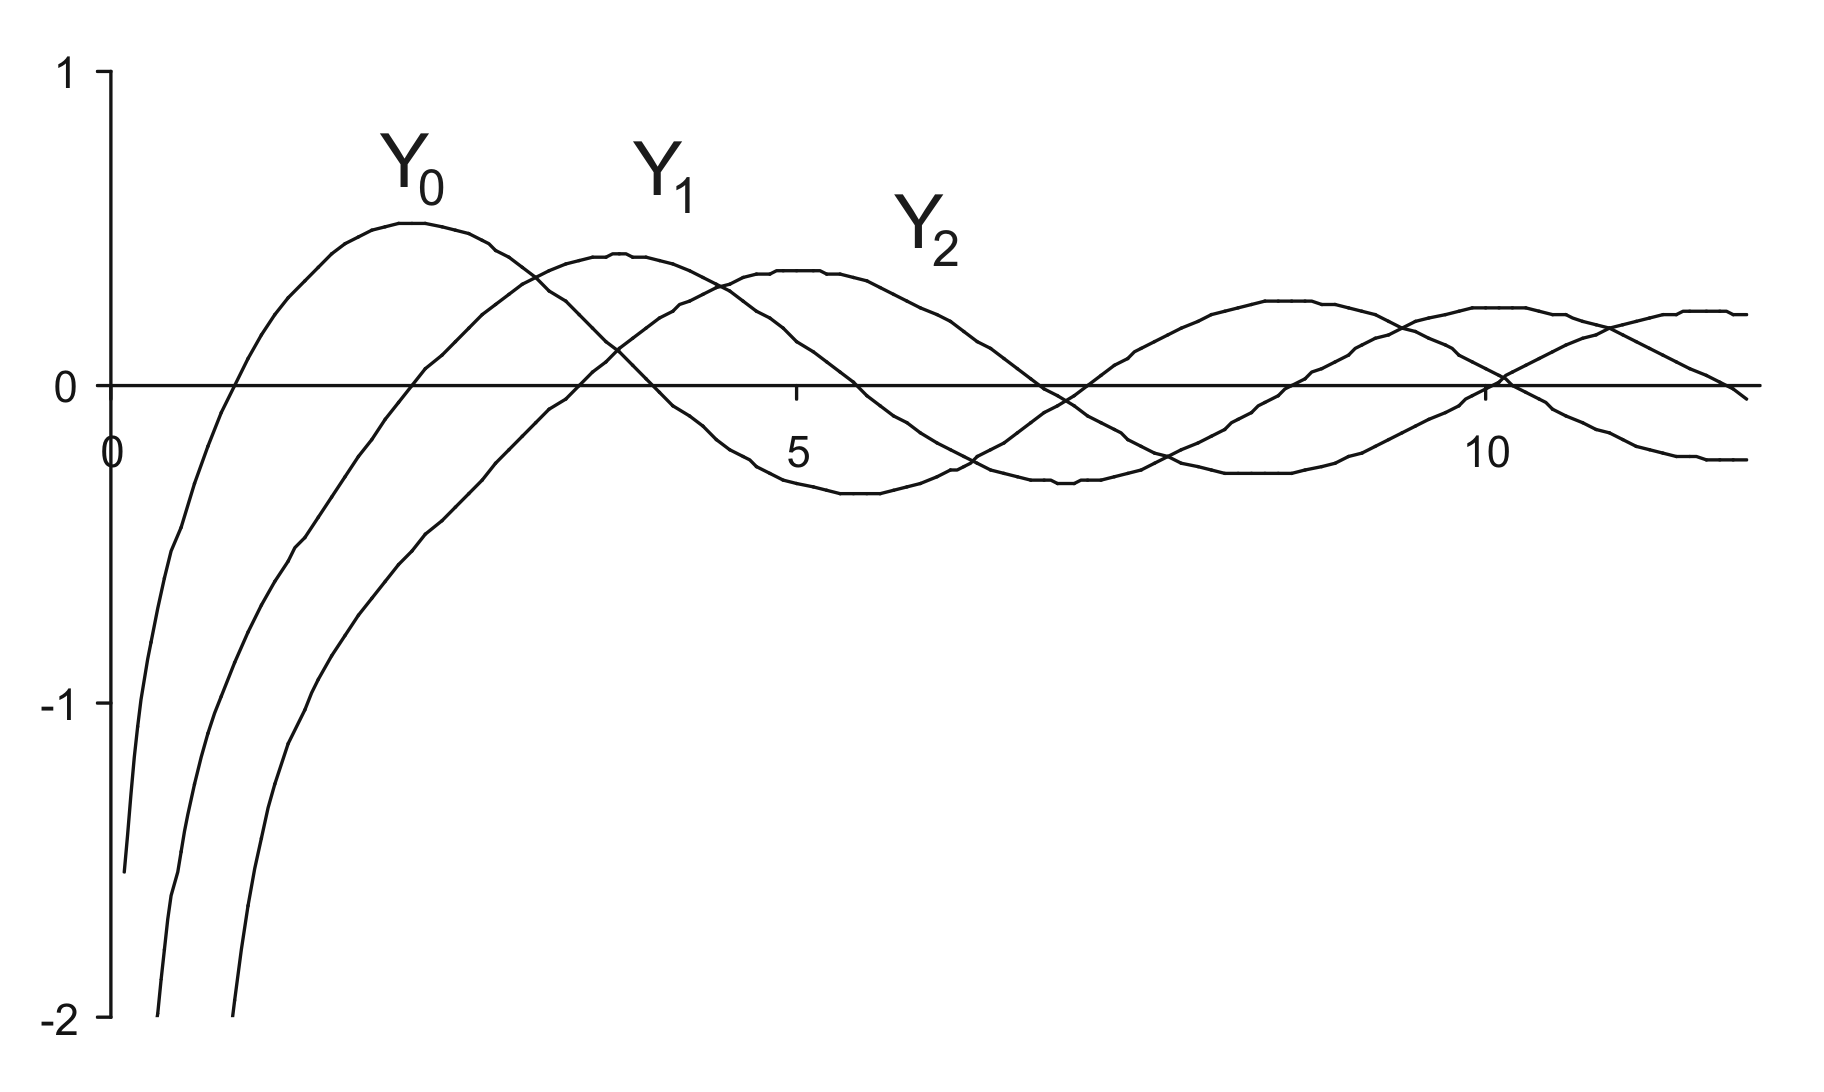
\includegraphics[scale=0.7]{special/figures/y}
\caption{The Neumann functions $Y_0(x)$, $Y_1(x)$ and $Y_2(x)$.}
\label{fig-bessel-Y}
\end{figure}

So the general solution of Bessel's equation can be written as

\begin{equation}
f(x) = A J_{\nu}(x) + B Y_{\nu}(x)
\end{equation} 

Of course, any other linearly independent combination of $J_{\nu}(x)$ and $Y_{\nu}(x)$ can also be used to express the solution, e.g.

\begin{equation}
f(x) = C H_{\nu}^{(1)}(x) + D H_{\nu}^{(2)}(x)
\end{equation} 

Here, $H_{\nu}^{(1)}(x)$ and $H_{\nu}^{(2)}(x)$ are the \emph{Hankel} functions of the first and second kind respectively, defined by

\begin{subequations}
\begin{equation}
\fbox{$\displaystyle H_{\nu}^{(1)}(x) = J_{\nu}(x) + j Y_{\nu}(x)$}
\end{equation} 
\begin{equation}
\fbox{$\displaystyle H_{\nu}^{(2)}(x) = J_{\nu}(x) - j Y_{\nu}(x)$}
\end{equation} 
\label{eq-hankel}
\end{subequations} 

Of course, if we are solving Eq.~\ref{eq-helmholtz-cyl} instead of Eq.~\ref{eq-bessel}, the arguments of the functions above are $k_t r$ instead of $x$. It is instructive to compare these functions to the solutions of the Helmholtz equation in a 1D Cartesian coordinate system:

\begin{equation}
f''(x) + k^2 f(x) = 0 \label{eq-helmholtz-1D}
\end{equation} 

The solutions of Eq.~\ref{eq-helmholtz-1D} are

\begin{equation}
f(x) = A \cos(kx) + B \sin(kx)
\end{equation} 

The sine and cosine solutions are oscillating solutions which can be interpreted physically as standing waves. Note the correspondence to $J_n(x)$ and $Y_n(x)$ which are also oscillating functions. Therefore, they can be thought of as the representation of standing waves in a circular coordinate system, with the only difference that $Y_n(x)$ diverges at the origin.

Another way of writing the solutions of Eq.~\ref{eq-helmholtz-1D} is

\begin{equation}
f(x) = C e^{jkx} + D e^{-jkx}
\end{equation} 

because $e^{\pm j \theta} = \cos \theta \pm j \sin \theta$ (compare this to Eq.~\ref{eq-hankel}).

Physically, $e^{-jkx}$ corresponds to an outgoing wave travelling towards $x=+\infty$, while $e^{jkx}$ is an incoming wave from $x=+\infty$ \footnote{This is for a choice of $e^{j \omega t}$ as time dependence in the definition of phasors. Some authors choose $e^{-j \omega t}$ as time dependence, and then $e^{-jkx}$ is an incoming wave.}.

It can be proven that for large $x$ the following asymptotic expansions hold:
$H_{\nu}^{(1)}(x) \sim e^{jx}$ and  $H_{\nu}^{(2)}(x) \sim e^{-jx}$. So, $H_{\nu}^{(2)}(x)$ is the cylindrical equivalent of an outgoing plane wave, while $H_{\nu}^{(1)}(x)$ is an incoming plane wave.

Whether to use Bessel/Neumann functions or rather Hankel functions to represent the solution of Bessel's differential equation, is usually determined by physical and/or practical considerations, as we will illustrate next for the case of finding eigenmodes in an optical fibre.

\sectionugent{Application: the eigenmodes of an optical fibre}

Consider the optical fibre from Fig.~\ref{fig-fibre}: a central core with radius $R$ made of a material with refractive index $n_1$, surrounded by a cladding with refractive index $n_2 < n_1$. The cladding is taken to be infinitely thick. 

\begin{figure}
\centering
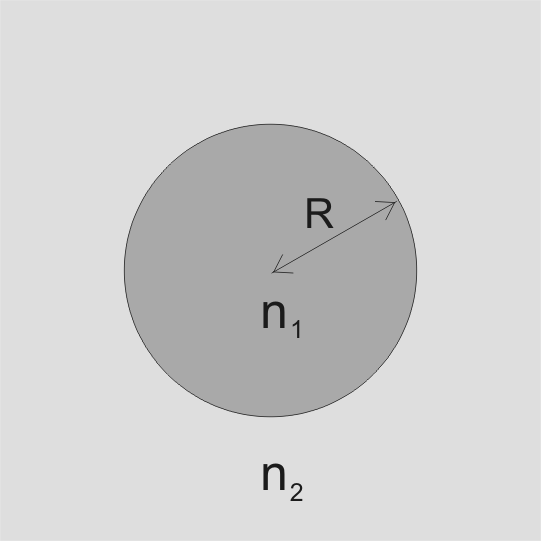
\includegraphics{special/figures/fibre}
\caption{Optical fibre.}
\label{fig-fibre}
\end{figure}

Fields in the optical fibre have to satisfy the Helmholtz equation. Just like in Section~\ref{sec-bessel-eq}, we propose solutions of the form 

\begin{equation}
\psi(r,\theta,z) = R(r)e^{-j k_\theta \theta }e^{-j k_z z} \\
\end{equation}  

These kinds of solutions are actually the eigenmodes of this particular waveguide, because of the form of their $z$--dependence\footnote{These eigenmodes propagate along $z$. Contrast this with the treatment of bent waveguides in the previous chapter, where the $z$--dimension didn't come in play because of the 2D nature of the problem and where the propagation was essentially along $\theta$.}.  Also, the fields must be periodic in the $\theta$--direction with period $2 \pi$. This means $k_\theta$ has to be an integer, which we will call $l = 0, \pm 1, \pm 2, \ldots$.

As we've seen before, $R$ has to satisfy this equation:

\begin{equation}
r^2\frac{d^2 R(r)}{d r^2} + r \frac{d R(r)}{d r} + \left[{r^2 \left(k_0^2 n^2(r) - k_z^2\right) - l^2}\right]R(r) = 0 \label{eq-fibre-0}
\end{equation} 

We define $k_{t,i}^2=k_0^2 n_i^2 - k_z^2$, where $i=1$ for the core and $i=2$ for the cladding.

We already know that in each of the regions $i$ the solutions of Eq.~\ref{eq-fibre-0} are Bessel functions of order $l$ with argument $k_{t,i} r$.

For the core, we write the general solution as

\begin{equation}
R(r) = A J_l\left(k_{t,1}r\right) + B Y_l\left(k_{t,1}r\right), \hspace{0.5 cm} r<R \label{eq-fibre-1}
\end{equation} 

But since the Neumann functions diverge at $r=0$, it immediately follows that $B=0$.

For the cladding, it is more advantageous to write the general solution in terms of Hankel functions:

\begin{equation}
R(r) = C H_l^{(1)}\left(k_{t,2}r\right) + D H_l^{(2)}\left(k_{t,2}r\right), \hspace{0.5 cm} r>R \label{eq-fibre-2}
\end{equation} 

For physical reasons, there can only be outgoing waves towards infinity, so $C=0$. Note that contrary to $k_{t,1}$, $k_{t,2}$ is imaginary for $k_0 n_2 < k_z < k_0 n_1$, so the fields for guided modes are exponentially decaying in the cladding.

So far, the treatment has been fully vectorial because solutions of the form (\ref{eq-fibre-1}) and (\ref{eq-fibre-2}) have to written both for $E_z$ and $H_z$, and these two fields couple because of the continuity conditions at $r=R$. For the sake of simplicity, we will only consider a scalar approximation here, where the modes are approximately TEM and the continuity conditions are simplified to the continuity of $R$ and $d R / d r$. This approximation turns out to be valid for weakly guided fibres where $n_1 \approx n_2$.

Imposing the continuity of $R$ and $d R / dr$ leads to

\begin{equation}
A J_l\left(k_{t,1}R\right) = D H_l^{(2)}\left(k_{t,2}R\right)
\end{equation} 

\begin{equation}
A k_{t,1} J'_l\left(k_{t,1}R\right) = D k_{t,2} H_l'^{(2)}\left(k_{t,2}R\right)
\end{equation} 

This only has non--trivial solutions if

\begin{equation}
\frac{J_l\left(k_{t,1}R\right)}{k_{t,1} J'_l\left(k_{t,1}R\right)} = \frac{H_l^{(2)}\left(k_{t,2}R\right)}{k_{t,2} H_l'^{(2)}\left(k_{t,2}R\right)} \label{eq-disp-fibre}
\end{equation}

Since $k_{t,1}$ and $k_{t,2}$ are functions of $k_z$, Eq.~\ref{eq-disp-fibre} can be used to calculate the $k_z$'s of the eigenmodes of the fibre. After that, the field profiles can be calculated from Eq.~\ref{eq-fibre-1} and \ref{eq-fibre-2}.

\begin{sidebar}
\begin{ex}
Solve the Helmholtz equation in free space in cylindrical coordinates. Look at the evolution of the intensity of the solution as a function of $z$. What do you notice? These modes are called \emph{Bessel beams}.
\end{ex}
\end{sidebar}


\pagebreak


\sectionugent{Hermite's differential equation}

In the Bachelor's level Photonics course, Gaussian beams were introduced as solutions to the paraxial wave equation. We will briefly review this material, and then go on to look for higher--order solutions to this equation. In this process, Hermite polynomials will pop up and we will study their properties as a model for other orthogonal polynomials.

The paraxial wave equation is an approximation to the Helmholtz equation under the so--called slowly varying envelope approximation (SVEA). This approximation looks for solutions which are essentially plane waves propagating along the $z$--direction, but which are modulated by a slowly varying function $A({\bf r})$:

\begin{equation}
\psi({\bf r}) = A({\bf r})e^{-jkz}
\end{equation} 

So,

\begin{equation}
\frac{\partial \psi({\bf r})}{\partial z} = \frac {\partial A({\bf r})}{\partial z}e^{-jkz} -j k A({\bf r})e^{-jkz}
\end{equation} 

and

\begin{equation}
\frac{\partial^2 \psi({\bf r})}{\partial z^2} = \frac{\partial^2 A({\bf r})}{\partial z^2}e^{-jkz} - 2 j k \frac{\partial A({\bf r})}{\partial z}e^{-jkz} - k^2 A({\bf r})e^{-jkz}
\end{equation} 

The fact that $A({\bf r})$ is a slowly varying function of $z$ means that we can neglect $\partial^2 A / \partial z^2$ with respect to $j k \partial A / \partial z$in the previous equation. With this, the Helmholtz equation reduces to

\begin{equation}
\fbox{$\displaystyle
\nabla_T^2 A({\bf r}) -2jk \frac{\partial A({\bf r})}{\partial z} = 0
$}
\label{eq-paraxial}
\end{equation} 

Here, $\nabla_T^2$ stands for the transverse part $(\partial^2 / \partial x^2) + (\partial^2 / \partial y^2)$ of the Laplacian operator.

A solution to this equation is the Gaussian beam, which is given by

\begin{equation}
A_G({\bf r}) = \frac{1}{q(z)}e^{-\frac{jk\rho^2}{2q(z)}} \label{eq-gauss}
\end{equation}   

where $q(z)=z+jb_0$. 

In this context, the function $W(z)$ is defined as

\begin{equation}
W(z)=\sqrt{\frac{2 b_0}{k} \left(1 + \frac{z^2}{b_0^2}\right)} \label{eq-W}
\end{equation} 

$W(z)$ can be interpreted as the beam width of the Gaussian beam.

\subsection*{Higher--order solutions of the paraxial wave equation}

Let's try to find a modulated version of the Gaussian beam which also satisfies the paraxial wave equation:

\begin{equation}
A(x,y,z) = X\left({\frac{\sqrt{2}x}{W(z)}}\right) Y\left({\frac{\sqrt{2}y}{W(z)}}\right) e^{-jZ(z)} A_G(x,y,z) \label{eq-gauss-higher}
\end{equation} 

Here, $A_G$ is the Gaussian beam from Eq.~\ref{eq-gauss} and $X()$, $Y()$ and $Z()$ are three real--valued functions that we still need to determine such that Eq.~\ref{eq-gauss-higher} satisfies the paraxial Helmholtz equation.

For the derivatives of Eq.~\ref{eq-gauss-higher} we get

\begin{equation}
\frac{\partial A}{\partial x} = \frac{\sqrt{2}}{W}X'Ye^{-jZ} A_G + XYe^{-jZ} \frac{\partial A_G}{\partial x} 
\end{equation} 

and

\begin{equation}
\frac{\partial^2 A}{\partial x^2} = \frac{2}{W^2}X''Ye^{-jZ} A_G  + 2\frac{\sqrt{2}}{W}X'Ye^{-jZ} \frac{\partial A_G}{\partial x}  + XYe^{-jZ} \frac{\partial^2 A_G}{\partial x^2}
\end{equation} 

Or, using Eq.~\ref{eq-gauss} to calculate $\partial A_G / \partial x$:

\begin{equation}
\frac{\partial^2 A}{\partial x^2} = \frac{2}{W^2}X''Ye^{-jZ} A_G  - 2j k x \frac{\sqrt{2}}{qW}X'Ye^{-jZ}A_G  + XYe^{-jZ} \frac{\partial^2 A_G}{\partial x^2} \label{eq-hermite-gauss-1}
\end{equation} 

and similar equations for the $y$--derivatives. For the $z$--derivative we get

\begin{align}
\frac{\partial A}{\partial z} =  -\frac{\sqrt{2}x W'}{W^2}X'Ye^{-jZ} A_G -\frac{\sqrt{2}y W'}{W^2}XY'e^{-jZ} A_G \nonumber \\ 
+ XY\left(-jZ'\right)e^{-jZ} A_G + XYe^{-jZ}\frac{\partial A_G}{\partial z} \label{eq-hermite-gauss-2}
\end{align} 

Let's substitute this in the paraxial equation Eq.~\ref{eq-paraxial}. Because $A_G$ is itself a solution of this equation, the last terms from Eq.~\ref{eq-hermite-gauss-1} and \ref{eq-hermite-gauss-2} cancel and we get:

\begin{align}
\frac{2}{W^2}\left(X''Y+XY''\right)e^{-jZ} A_G   \nonumber \\
-2jk \frac{\sqrt{2}}{Wq}\left(xX'Y+yXY'\right)e^{-jZ}A_G \nonumber \\
+2jk \frac{\sqrt{2} W'}{W^2}\left(xX'Y+yXY'\right)e^{-jZ}A_G \nonumber \\
-2jk XY\left(-jZ'\right)e^{-jZ} A_G = 0
\end{align}

Getting rid of the common factors and dividing by $XY$, we get

\begin{equation}
\frac{1}{W^2}\left(\frac{X''}{X}+\frac{Y''}{Y}\right)  
- j k \left(\frac{\sqrt{2}}{Wq} - \frac{\sqrt{2}W'}{W^2}\right)\left(x\frac{X'}{X}+y\frac{Y'}{Y}\right)
-kZ' = 0
\end{equation} 

or
\begin{equation}
\left(\frac{X''}{X}+\frac{Y''}{Y}\right)  
- j k  \left(\frac{W^2}{q} - W'W\right)\frac{\sqrt{2}}{W}\left(x\frac{X'}{X}+y\frac{Y'}{Y}\right)
-kW^2Z' = 0
\end{equation} 

Using the definitions for $W$ and $q$, it follows that $W^2/q - W'W = -j \lambda / \pi$. If we now perform the change of variables $u = \sqrt(2) x / W(z)$ and  $v = \sqrt(2) y / W(z)$, we get

\begin{equation}
\left[{\frac{X''(u)}{X(u)} - 2 u\frac{X'(u)}{X(u)}}\right] + 
\left[{\frac{Y''(v)}{Y(v)} - 2 v\frac{Y'(v)}{Y(v)}}\right] -kW^2(z)Z'(z) = 0
\end{equation} 

The left--hand side of this equation is a sum a three terms, each of which is a function of a single independent variable ($u$, $v$ and $z$ respectively). Therefore, each of these terms must be equal to a constant. Equating the first term to $-2\mu_1$ and the second to $-2\mu_2$, the third must be equal to $2(\mu_1+\mu_2)$. This separation of variables leads to the following ordinary differential equations:

\begin{equation}
X''(u) - 2 u X'(u) = - 2 \mu_1 X(u) \label{eq-diff-hermite-0}
\end{equation} 

\begin{equation}
Y''(v) - 2 v Y'(v) = - 2 \mu_2 Y(v)
\end{equation} 

\begin{equation}
b_0\left(1 + \frac{z^2}{b_0^2}\right)Z'(z) = -(\mu_1+\mu_2)
\end{equation} 

From this, it follows immediately that $Z(z) = -(\mu_1+\mu_2) \arctan(z/b_0)$. However, the differential equations for $X$ and $Y$ have no obvious solutions at first sight. In the next sections, we will show that their solutions are \emph{Hermite polynomials}, and that $\mu_1$ and $\mu_2$ are integers.

In similar vein to the treatment of Bessel functions, we will start by introducing a generating function and then continue to derive recurrence relations which will lead to a differential equation.

\sectionugent{Generating function for Hermite polynomials}

The generating function of the Hermite polynomials takes the following form:

\begin{equation}
g(x,t) = e^{-t^2 + 2tx} \label{eq-gen-hermite}
\end{equation}

The Hermite polynomials $H_n(x)$ are \emph{defined} from the the Laurent series in $t$ of $g(x,t)$ as 

\begin{equation}
e^{-t^2 + 2tx}= \sum_{n = 0}^{\infty} H_n(x)\frac{t^n}{n!} \label{eq-g-hermite}
\end{equation} 

Note the absence of a superscript in $H_n(x)$, which distinguishes them from the unrelated Hankel functions.

\begin{sidebar}
\begin{ex}
Show that
$$H_n(x) = \sum_{r=0}^{\lfloor n/2 \rfloor}(-1)^r {(2x)}^{n-2r} \frac{n!}{(n-2r)! r!}$$
\end{ex}
\end{sidebar}

\sectionugent{Recurrence relations for Hermite polynomials}

Similar to the treatment of Bessel functions, we can derive recurrence relations by differentiating the generating function.

E.g. by differentiating Eq.~\ref{eq-g-hermite} with respect to $t$, we get

\begin{equation}
(-2t+2x)e^{-t^2 + 2tx} = \sum_{n = 0}^{\infty} H_n(x) \frac{nt^{n-1}}{n!}
\end{equation} 

Substituting Eq.~\ref{eq-g-hermite} back in this, we get

\begin{equation}
(-2t+2x) \sum_{n = 0}^{\infty} H_n(x)\frac{t^n}{n!} = \sum_{n = 0}^{\infty} H_n(x) \frac{nt^{n-1}}{n!}
\end{equation} 

This leads to

\begin{equation}
-2  \frac{H_{n-1}(x)}{(n-1)!} + 2 x \frac{H_n(x)}{n!} = H_{n+1}(x) \frac{n+1}{(n+1)!}
\end{equation} 

where $n \geq 1$, or

\begin{equation}
\fbox{$\displaystyle
H_{n+1}(x) = 2 x H_n(x) - 2 n H_{n-1}(x)
$} \label{eq-recur-hermite-1}
\end{equation} 

Direct expansion of the generating function yields that $H_0(x) = 1$ and that $H_1(x) = 2x$. With this and Eq.~\ref{eq-recur-hermite-1}, we can iteratively construct all the Hermite polynomials. For reference, Table \ref{tab-hermite} lists the first Hermite polynomials. Fig.~\ref{fig-hermite} plots the first three Hermite polynomials.

\begin{figure}
\centering
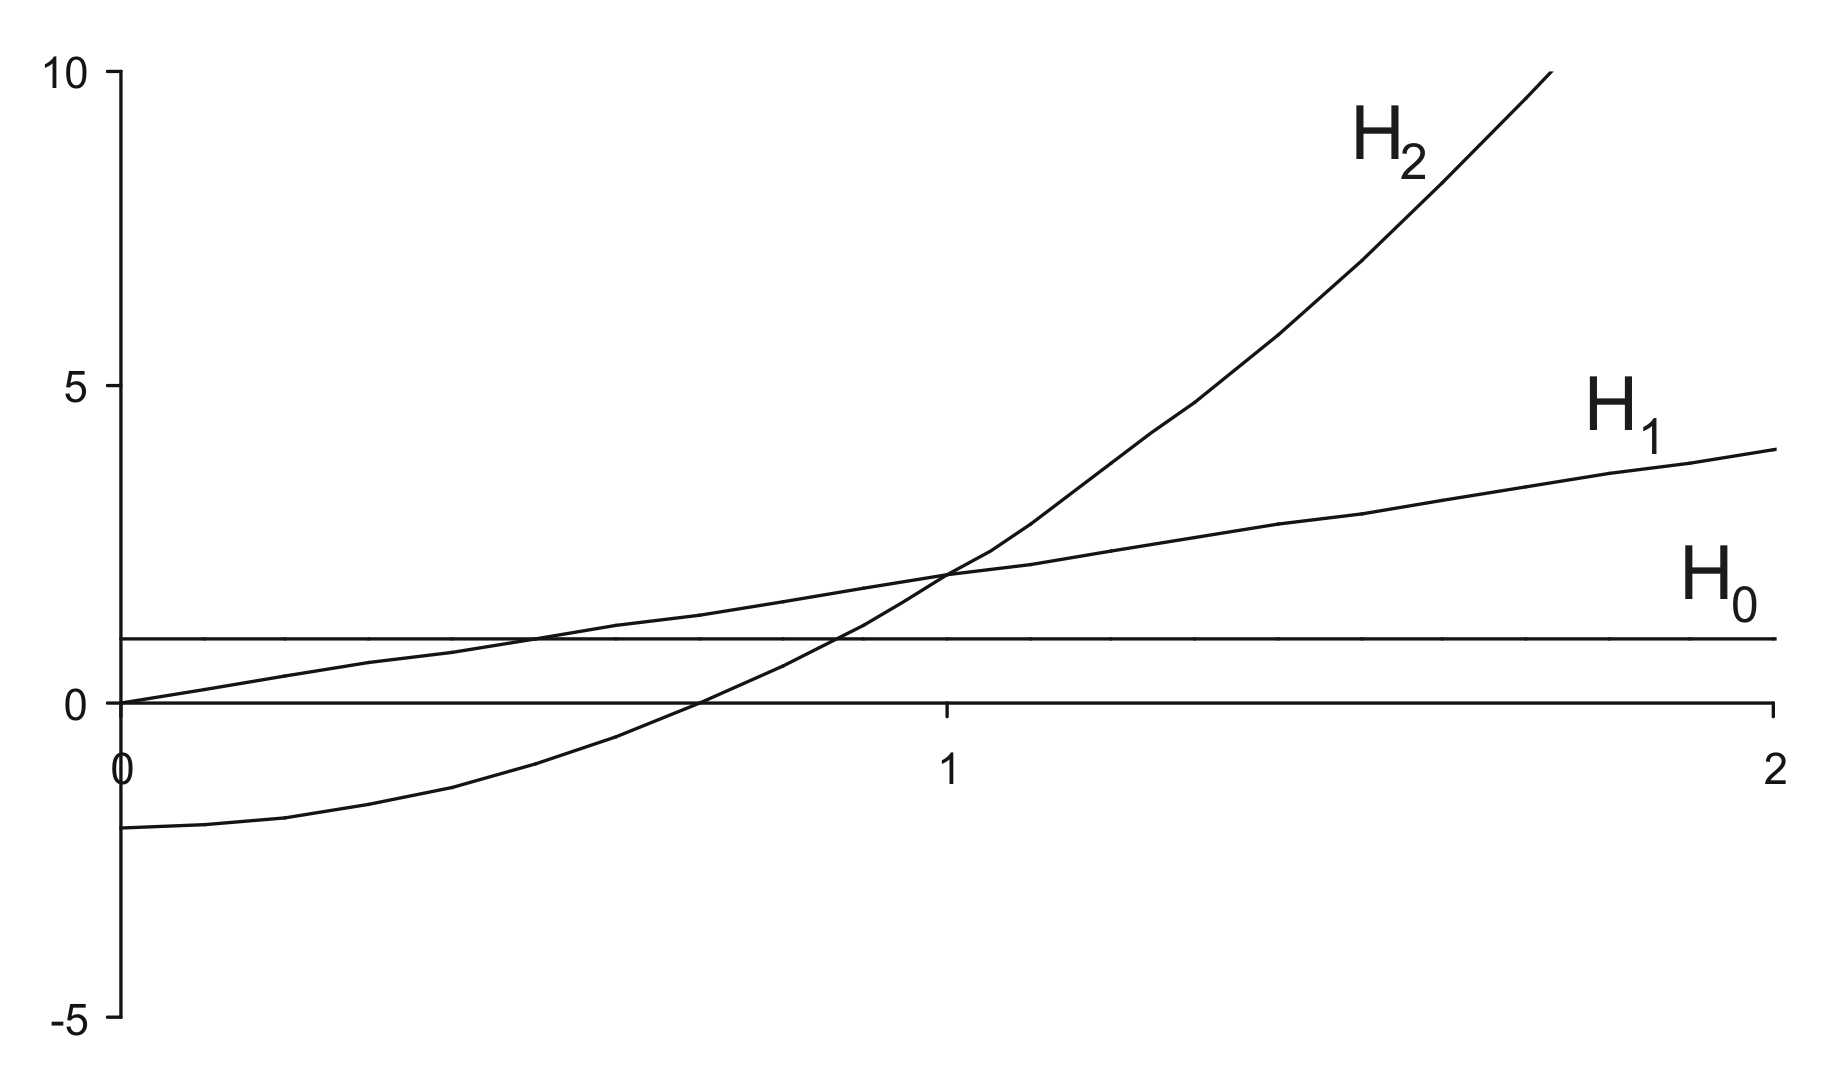
\includegraphics[scale=0.7]{special/figures/hermite}
\caption{The Hermite polynomials $H_0(x)$, $H_1(x)$, $H_2(x)$.}
\label{fig-hermite}
\end{figure}

\begin{table}
\begin{align}
H_0(x) = & 1 \nonumber \\
H_1(x) = & 2x \nonumber \\
H_2(x) = & 4x^2-2 \nonumber \\
H_3(x) = & 8x^3-12x \nonumber \\
H_4(x) = & 16x^4-48x^2+12 \nonumber \\
H_5(x) = & 32x^5-160x^3+120x \nonumber \\
H_6(x) = & 64x^6-480x^4+720x^2-120 \nonumber
\end{align}
\caption{Hermite polynomials}
\label{tab-hermite}
\end{table}  

\begin{sidebar}
\begin{ex}
Show that
$$\fbox{$\displaystyle H_n'(x) = 2nH_{n-1}(x)$}$$ \label{eq-recur-hermite-2}
\end{ex}
\end{sidebar}

\sectionugent{Hermite's differential equation revisited}

Differentiating Eq.~\ref{eq-recur-hermite-1} with respect to $x$, we get

\begin{equation}
H_{n+1}'(x) = 2  H_n(x) + 2 x H_n'(x)- 2 n H_{n-1}'(x)
\end{equation} 

Using the results from  Ex. \ref{eq-recur-hermite-2}, we have $H_{n+1}'(x) = 2(n+1)H_n(x)$ and $2 n H_{n-1}'(x) = H_n''(x)$:

\begin{equation}
2(n+1)H_n(x) = 2  H_n(x) + 2 x H_n'(x)- H_n''(x)
\end{equation} 

This reduces to

\begin{equation}
\fbox{$\displaystyle
H_n''(x) - 2 x H_n'(x) + 2n H_n(x) = 0 \label{eq-diff-hermite-1}
$}
\end{equation} 

which is indeed Eq.~\ref{eq-diff-hermite-0}, with $\mu_1=n$.

Returning to our higher--order solutions of the paraxial wave equation, Fig.~\ref{fig-gauss-hermite} plots the field profile of some of these so--called \emph{Gauss--Hermite modes}. They are characterised by two integer indices, indicating the order of the Hermite polynomials for the $x$ and $y$ direction.

\begin{figure}
\centering
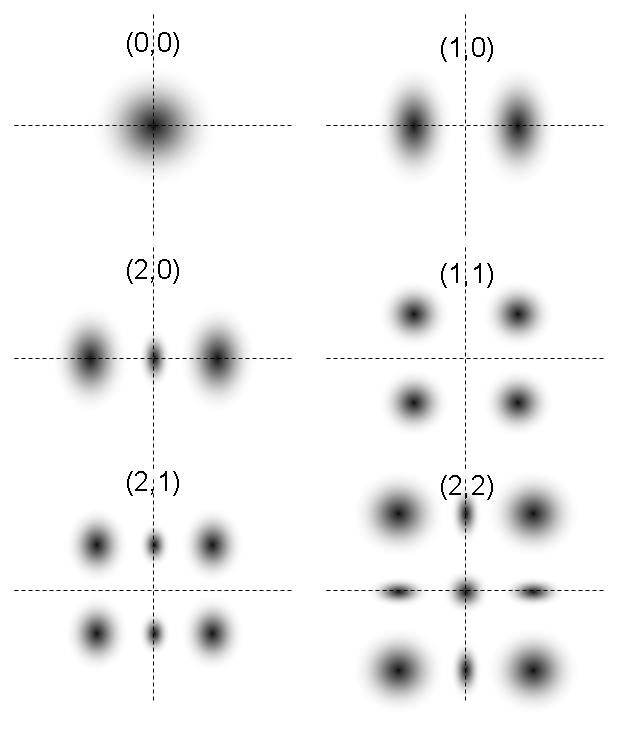
\includegraphics[scale=0.5]{special/figures/gauss}
\caption{Some Gauss--Hermite modes.}
\label{fig-gauss-hermite}
\end{figure}

\sectionugent{Series expansion using Hermite polynomials}

Just as we did with Bessel functions, we can use Hermite polynomials to expand a function in a series. In order to do that, we will need to establish the correct orthogonality relation between Hermite polynomials and normalise them.

Consider the following two differential equations:

\begin{equation}
\phi'' - 2 x \phi' + 2m \phi = 0 \label{eq-hermite-ortho-1}
\end{equation}
\begin{equation}
\psi'' - 2 x \psi' + 2n \psi = 0 \label{eq-hermite-ortho-2}
\end{equation}

The solutions of these are $H_m(x)$ and $H_n(x)$ respectively. Multiplying Eq.~\ref{eq-hermite-ortho-1} by $\psi e^{-x^2}$, Eq.~\ref{eq-hermite-ortho-2} by $\phi e^{-x^2}$ and subtracting, we get

\begin{equation}
e^{-x^2}\left(\phi''\psi -\psi''\phi\right)- e^{-x^2} 2 x \left(\phi'\psi -\psi'\phi\right)+ e^{-x^2}2(m-n)\phi\psi = 0
\end{equation} 

This can be written as

\begin{equation}
\left[e^{-x^2}\left(\phi'\psi -\psi'\phi\right)\right]' = e^{-x^2}2(n-m)\phi\psi
\end{equation} 

Integrating this between $-\infty$ and $\infty$ we get

\begin{equation}
2(n-m)\int_{-\infty}^{\infty}e^{-x^2}\phi\psi dx = \left[e^{-x^2}\left(\phi'\psi -\psi'\phi\right)\right]_{-\infty}^{+\infty}
\end{equation} 

The right hand side is equal to zero, because $e^{-{\infty}^2}$ goes to zero more quickly than any polynomial.

So in the end we get

\begin{equation}
\fbox{$\displaystyle
\int_{-\infty}^{\infty}e^{-x^2}H_n(x)H_m(x)dx = 0, \hspace{0.5cm} n \ne m \label{eq-hermite-ortho}
$}
\end{equation} 

This is the orthogonality relation for Hermite polynomials: they are orthogonal over the interval $[-\infty, \infty]$ with the weighting function $e^{-x^2}$.


To normalise the Hermite polynomials, we need to calculate

\begin{equation}
I = \int_{-\infty}^{\infty}e^{-x^2}H_n^2(x)dx
\end{equation}

We do this by multiplying the generating function Eq.~\ref{eq-g-hermite} by itself and by  $e^{-x^2}$:

\begin{equation}
e^{-x^2} e^{-t^2 + 2tx} e^{-s^2 + 2sx}= \sum_{m, n = 0}^{\infty}e^{-x^2} H_n(x)\frac{t^n}{n!}H_m(x)\frac{s^m}{m!}
\end{equation} 

When we integrate this over $x$ from $-\infty$ to $\infty$, the terms with $m \ne n$ on the right--hand side drop out because of the orthogonality relation Eq.~\ref{eq-hermite-ortho}:

\begin{equation}
\int_{-\infty}^{\infty} e^{-x^2} e^{-t^2 + 2tx} e^{-s^2 + 2sx} dx= \sum_{n = 0}^{\infty} \int_{-\infty}^{\infty} e^{-x^2} H_n^2(x)\frac{(st)^n}{n!n!} dx \label{eq-hermite-norm-1}
\end{equation} 

For the integral on the left--hand side, we get \footnote{To calculate $\int_{-\infty}^{\infty}e^{-x^2}dx$, write it as $\sqrt{\int_{-\infty}^{\infty} e^{-x^2}dx\int_{-\infty}^{\infty} e^{-y^2}dy}$ and transform it to polar coordinates with $x^2+y^2=r^2$ and $dxdy = r dr d\theta$.}

\begin{align}
\int_{-\infty}^{\infty} e^{-x^2} e^{-t^2 + 2tx} e^{-s^2 + 2sx} dx 
  = & \int_{-\infty}^{\infty} e^{-(x-s-t)^2} e^{2st}dx \nonumber \\
  = & \sqrt{\pi} e^{2st} \nonumber \\
  = & \sqrt{\pi} \sum_{n = 0}^{\infty} \frac{2^n{(st)}^n}{n!}  \label{eq-hermite-norm-2}
\end{align} 

By equating like powers of $st$ in the the right--hand sides of Eq.~\ref{eq-hermite-norm-1} and \ref{eq-hermite-norm-2} we get the value of the normalisation integral:

\begin{equation}
\int_{-\infty}^{\infty} e^{-x^2} H_n^2(x) dx = 2^n n! \sqrt{\pi}
\end{equation} 

With this we can finally write the complete expression to expand a function $f(x)$ in a series of Hermite polynomials:

\begin{equation}
f(x) = \sum_{n=0}^{\infty}a_n H_n(x)
\end{equation} 

with

\begin{equation}
\fbox{$\displaystyle
a_n = \frac{1}{2^n n!\sqrt{\pi}} \int_{-\infty}^{\infty} e^{-x^2} H_n(x) f(x) dx
$}
\end{equation} 


\begin{sidebar}
\begin{ex}
Prove the following parity relation:
$$H_n(x) = (-1)^nH_n(-x)$$
a) by using the series expansion of Hermite polynomials
b) by replacing $t$ by $-t$ and $x$ by $-x$ in the generating function
\end{ex}
\end{sidebar}

\begin{sidebar}
\begin{ex}
Use the definition of the generating function for Hermite polynomials to prove that
$$H_{2n}(0) = (-1)^n \frac{(2n)!}{n!}$$
$$H_{2n+1}(0) = 0$$
\end{ex}
\end{sidebar}

\begin{sidebar}
\begin{ex}
Prove the Rodriguez formula for Hermite polynomials:
$$H_n(x) = (-1)^n e^{x^2}\frac{d^n}{d x^n}\left(e^{-x^2}\right)$$
\emph{Hint}: verify this formula for a few values of $n$ to get a feeling for how it works, and then use mathematical induction.
\end{ex}
\end{sidebar}

\begin{sidebar}
\begin{ex}
For $0 \leq m \leq n-1$, use the Rodriguez formula to show that 
$$\int_{-\infty}^{\infty}x^m e^{-x^2} H_n(x) dx = 0$$
\end{ex}
\end{sidebar}

\begin{sidebar}
\begin{ex}
Prove that 
$$ | H_n(x) | \le  | H_n(jx) | $$
\emph{Hint}: remove factors from the series expansion of $ H_n(jx) $ so that it contains only positive terms.
\end{ex}
\end{sidebar}


\begin{sidebar}
\begin{ex}
Show that 
$$\left( 2x - \frac{d}{dx} \right)^n 1 = H_n(x)$$
\emph{Hint}: verify this formula for a few values of $n$ to get a feeling for how it works, and then use mathematical induction.
\end{ex}
\end{sidebar}

\begin{sidebar}
\begin{ex}
Show that
$$ \int_{-\infty}^{\infty} e^{-x^2} x^2 H_n^2(x) dx = 2^{n-1} (2n + 1) n! \sqrt{\pi} $$
\emph{Hint}: expand $x H_n(x)$ using a recurrence relation and apply the orthogonality conditions.
This integral occurs in the calculation of the mean-square displacement of a quantum oscillator.
\end{ex}
\end{sidebar}

\begin{sidebar}
\begin{ex}
Expand the following integral in a power series in $t$

$$ \int_{-\infty}^{\infty} e^{-x^2/2} g(x,t) dx$$

and use the result to show that

$$\int_{-\infty}^{\infty} e^{-x^2/2} H_{2m}(x) dx = \frac{(2m)!}{m!} \sqrt{2\pi} $$
$$\int_{-\infty}^{\infty} e^{-x^2/2} H_{2m+1}(x) dx = 0 $$
\end{ex}
\end{sidebar}


\begin{sidebar}
\begin{ex}
Multiply the generating function by $t^{-k-1}$ and integrate over the unit circle in the complex $t$-plane to show that

$$H_k(x) =\frac{k!}{2 \pi j} \oint \frac{e^{-t^2 +2tx}}{t^{k+1}}dt $$

Then, show by direct substitution that this expression satisfies Hermite's differential equation. \emph{Hint}: try to write the integrand as a total differential.
\end{ex}
\end{sidebar}

\begin{sidebar}
\begin{ex}
Assume that based only on Hermite's differential equation, we managed to derive the recurrence relation involving $H_n'(x)$, as well as the values of $H_n(0)$. Based only on this information, derive the explicit form of the generating function $g(x,t)$ defined as

$$g(x,t) = \sum_{n = 0}^{\infty} H_n(x)\frac{t^n}{n!} $$

a) Take the derivative of $g(x,t)$ above with respect to $x$, use the recurrence relationship, and derive a first-order differential equation for $g(x,t)$.\\

b) Solve this equation to give

$$g(x,t) = e^{2tx} f(t)$$

c) Derive $f(t)$ by evaluating the expression for $x=0$.
\end{ex}
\end{sidebar}

\pagebreak
Friedrich Wilhelm Bessel (1784--1846)

%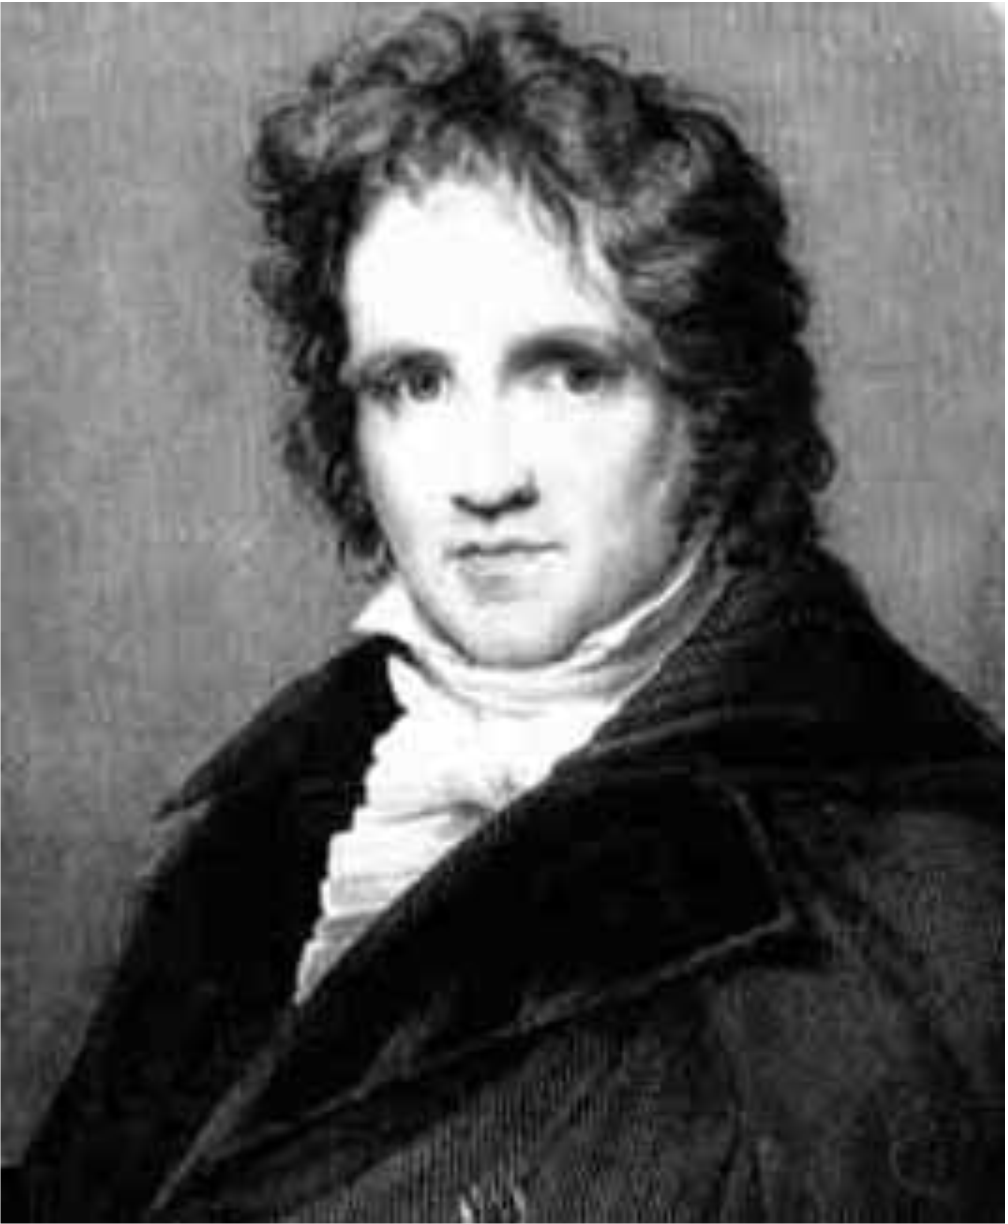
\includegraphics[scale=0.7]{special/figures/bessel}


%%% Local Variables:
%%% mode: latex
%%% TeX-master: "../main"
%%% End:

%\chapter{Numerical methods for photonics}
\label{h:numeric}

\begin{quote}
The purpose of computing is insight, not numbers.

--- Richard Hamming
\end{quote}

\begin{quote}
Understanding grows only logarithmically with the number of floating point operations 

--- J.P. Boyd
\end{quote}

\chaptertoc


In this chapter, we will briefly touch upon a number of techniques to numerically solve the wave equation in cases where no analytic solution is available. Four different classes of methods will be introduced.

First, in \textbf{finite difference} methods, we will replace continuous derivatives with discrete approximations on a grid. When applying this to the wave equation in the frequency domain, this results in a linear system, which can be solved in a number of ways. Doing this discretisation in the time domain results in the popular finite-difference time-domain method (FDTD).

The \textbf{finite element} method does not directly solve a differential equation. Rather, it tackles the problem obliquely by converting it into a minimisation procedure. This so-called variational approach has advantages when it comes to e.g. sensitivity to rounding errors.

\textbf{Eigenmode expansion} methods are used in layered photonic structures, in which the fields are expanded in the basis set formed by the eigenmodes of each layer. Thanks to this choice of basis functions that incorporate a lot of the physics of the problem, this approach can be very efficient.

Finally, a more abstract framework is presented, namely the \textbf{method of the weighted residuals}. This framework can be used to generalise a number of individual approaches, like point matching or the Galkerkin method.

Each of these subjects could be the topic of an entire course in its own right, so we will only be able to introduce the basic principle of these methods, without going into any level of detail. What is important however, is to get a feeling for each of these methods, to get to know their strengths and weaknesses, so that you can make the correct choice of tool for any given problem.


\pagebreak

\sectionyoutubeugent{Finite-difference approximation of derivatives}{KEirr8vynUI}

Let's say we are not interested in the solution to a certain differential equation in the entire domain of interest, but only in a limited number of discrete points inside the simulation domain. The set of discretisation points is called the \textbf{mesh}, and the distance between discretisation points is called the \textbf{mesh size}. A typical choice of 2D mesh is a rectangular one, where you only consider points of the form $(i \Delta x, j \Delta y)$, with $i$ and $j$ integers.

\begin{cue}
What do you think are some advantages and disadvantages of having a small mesh size?  
\end{cue}

Obviously the hope is that as the mesh becomes finer and finer, the solution that we obtain converges more and more to the true solution of the wave equation. However, the price we pay for this consists of increased computational resources (time, memory, ...).

\begin{marginfigure}[-2.0cm]
  % credits: Wikipedia
  % url: https://en.wikipedia.org/wiki/Brook_Taylor
  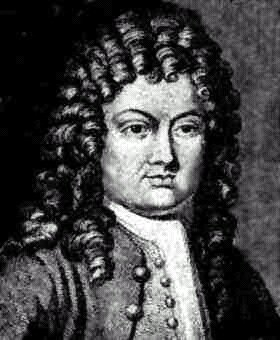
\includegraphics{numeric/figures/b_taylor}
  \caption{Brook Taylor (1685-1731)}
\end{marginfigure}

Since we only have information about the solution at discrete points, we will need to approximate the derivatives that appear in the differential equation using data from those discrete points. To write down these so--called \textbf{finite-difference} approximations for derivatives, we will develop e.g. an unknown 1D function $f(x)$ in a Taylor series.

\begin{cue}
\noindent\marginnote[2.0cm]{The symbol $\mathcal{O}$ relates to the \textbf{order} of the remaining terms, i.e. how they scale as a function of $\Delta x$. Here, $\mathcal{O}\left(\Delta x^4\right)$ should really be interpreted as $\mathcal{O}\left((\Delta x)^4\right)$, i.e. if the grid size becomes twice as small, the sum of the remaining terms becomes roughly 16 times as small.}Write down Taylor expansions of $f(x+\Delta x)$ and $f(x-\Delta x)$ up till the third derivative. 
\end{cue}

\begin{gather}
f(x+\Delta x) = f(x) + \Delta x \frac{d f}{d x} + \frac{{(\Delta x)}^2}{2} \frac{d^2 f}{d x^2} + \frac{{(\Delta x)}^3}{6} \frac{d^3 f}{d x^3} + \mathcal{O}\left(\Delta x^4\right) \label{eq-taylor-plus} \\
f(x-\Delta x) = f(x) - \Delta x \frac{d f}{d x} + \frac{{(\Delta x)}^2}{2} \frac{d^2 f}{d x^2} - \frac{{(\Delta x)}^3}{6} \frac{d^3 f}{d x^3} + \mathcal{O}\left(\Delta x^4\right) \label{eq-taylor-min}
\end{gather} 

\begin{cue}
Neglecting all the terms including $\left(\Delta x\right)^2$ or higher, use Eq.~\ref{eq-taylor-plus} to approximate the first derivative of $f$. How does the error term scale with $\Delta x$? 
\end{cue}

From Eq.~\ref{eq-taylor-plus} we get

\begin{equation}
\frac{d f}{d x} = \frac{f(x+\Delta x) - f(x)}{\Delta x} + \mathcal{O}\left(\Delta x\right)
\end{equation} 

This is called the \textbf{forward difference} approximation of $df / dx$. Since the error term is $\mathcal{O}(\Delta x)$ (note that in deriving the equation above, we needed to divide by $\Delta x$), this is called a first order approximation.

\begin{cue}
Do the same, but start from Eq.~\ref{eq-taylor-min}.
\end{cue}

Similarly from Eq.~\ref{eq-taylor-min}:

\begin{equation}
\frac{d f}{d x} = \frac{f(x) - f(x- \Delta x)}{\Delta x} + \mathcal{O}\left(\Delta x\right)
\end{equation} 

This so--called \textbf{backward difference} is also first--order accurate.

\begin{cue}
Now subtract Eq.~\ref{eq-taylor-plus} and Eq.~\ref{eq-taylor-min}. What is the order of accuracy of the approximation of the derivative now? Can you explain this intuitively?
\end{cue}

By subtracting Eq.~\ref{eq-taylor-plus} and Eq.~\ref{eq-taylor-min}, we get a \textbf{central difference} formula, which now however is second--order accurate, because the lower--order terms have cancelled:

\begin{equation}
\fbox{$\displaystyle
\frac{d f}{d x} = \frac{f(x + \Delta x) - f(x- \Delta x)}{2 \Delta x} + \mathcal{O}\left(\Delta x^2\right)
$}
\end{equation} 

This formula is second--order accurate thanks to the cancellation of terms in the Taylor expansion. Another way of looking at it is that the central difference involves not one but both neighbouring points, so it encorporates more information on the local behaviour of the function, which makes it more accurate.

\begin{marginfigure}
\centering
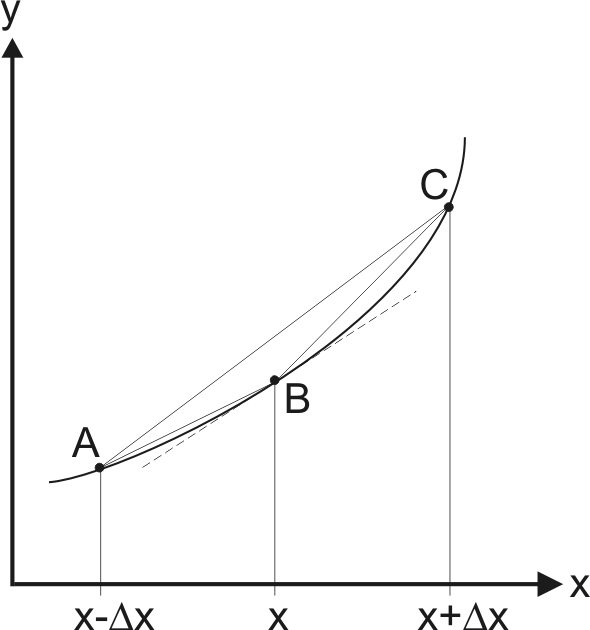
\includegraphics{numeric/figures/fd}
\caption{The arc AB represents backward differences, BC forward differences and AC central differences.}
\label{fig-fd}
\end{marginfigure}

Forward, backward and central differences are illustrated in Fig.~\ref{fig-fd}. From this figure, you can clearly see that the central difference is more accurate.


\begin{cue}
Construct an approximation for the second derivative $f''$, this time adding Eq.~\ref{eq-taylor-plus} and Eq.~\ref{eq-taylor-min}. What is the order of approximation? 
\end{cue}

By adding Eq.~\ref{eq-taylor-plus} and Eq.~\ref{eq-taylor-min}, we get an approximation for the second derivative:

\begin{equation}
\fbox{$\displaystyle
\frac{d^2 f}{d x^2} = \frac{f(x + \Delta x) -2 f(x) + f(x - \Delta x)}{ \Delta x^2} + \mathcal{O}\left(\Delta x^2\right)
$}
\end{equation} 

If we want to get more accurate results, we could either use a finer mesh or add more information by including higher order neighbours like $f(x-2\Delta x)$ and $f(x+2\Delta x)$.

Another way of looking at the second derivative is by rewriting the approximation as

\begin{equation}
\frac{d^2 f}{d x^2} \sim  \frac{f(x + \Delta x) + f(x - \Delta x)}{2} - f(x)
\end{equation}

\noindent\marginnote{Drawing a function with an inflection point, where $f''=0$, allows you to verify that there the function is indeed equal to the average of its surroundings.}This shows that the second derivative (or the Laplacian for that matter) is all about the difference between the value of a function at a certain point and the average value of that function around that point.

\begin{marginfigure}[1.0cm]
  % credits: Wikipedia
  % url: https://en.wikipedia.org/wiki/John_Crank
  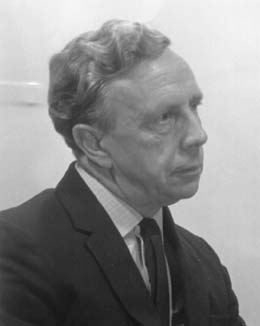
\includegraphics{numeric/figures/j_crank}
  \caption{John Crank (1916-2006)}
\end{marginfigure}

\begin{marginfigure}[8.5cm]
  % credits: Wikipedia
  % url: https://en.wikipedia.org/wiki/Phyllis_Nicolson
  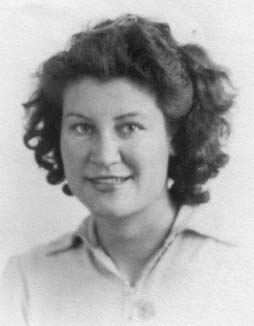
\includegraphics{numeric/figures/p_nicolson}
  \caption{Phyllis Nicolson (1917-1968)}
\end{marginfigure}

\begin{exer}
  % difficulty: normal
  % youtube: tU5OXUS6DxM
Construct a finite-difference scheme that will allow you to integrate the following differential equation:

$$\frac{du(t)}{dt} = -a u(t)$$

Calculate the approximations $u_n = u(n \Delta t)$ given an initial condition $u_0$ using several methods: \\

a) Approximate the time derivate using a forward difference. (This results in the forward Euler method.) \\

b) Same, but now use a backward difference. (This results in the backward Euler method.)\\

c) Construct a central difference at the intermediate time $t_{n+1/2}$ and eliminate $u_{n+1/2}$ by considering it to be the average of $u_{n}$ and $u_{n+1}$. (This results in the Crank-Nicholson method.) \\

d) Show that all of these methods can be formulated as one method (the $\theta$-rule):

$$u_{n+1} = \frac{1-(1-\theta) a \Delta t}{1+ \theta a \Delta t} u_n$$ \\

Which $\theta$-values correspond to which methods?

\end{exer}

\pagebreak

%\begin{exer}
% difficulty: normal
%Derive the following higher-order approximation of the second derivative:

%$$ \frac{d^2 f}{d x^2} = \frac{1}{12 \Delta x^2} \big[& -f(x + 2 \Delta x) + 16 f(x + \Delta x) -30 f(x) - f(x - 2 \Delta x) + 16 f(x- \Delta x) \big] + \mathcal{O}\left(\Delta x^4\right)$$

%\end{exer}


\begin{exer}
  % difficulty: normal
  % youtube: P6Fc_rOF_A0
Derive the following higher-order approximation of the second derivative:

\begin{align}  
  \frac{d^2 f}{d x^2} = \frac{1}{12 \Delta x^2} \big[& -f(x + 2 \Delta x) + 16 f(x + \Delta x) -30 f(x) \nonumber \\
  &  - f(x - 2 \Delta x) + 16 f(x- \Delta x) \big] + \mathcal{O}\left(\Delta x^4\right)
\end{align} 
\end{exer}


\pagebreak


\sectionyoutubeugent{Solving the 1D wave equation with finite differences}{TbIfp25tvQk}

Illustrating finite difference methods is best done using a simple example, so we will solve the 1D Helmholtz equation in a uniform medium:

\begin{equation}
\frac{d^2 f(x)}{d x^2} + k^2 f(x) = 0 \label{eq-helmholtz-1d}
\end{equation} 

We solve this problem at a fixed wavelength, i.e. a fixed value of $k$.

\begin{cue}
  Discretise this equation.
\end{cue}

The discretised version of Eq.~\ref{eq-helmholtz-1d} reads

\begin{equation}
\frac{f(x - \Delta x) -2 f(x) + f(x + \Delta x)}{ \Delta x^2} + k^2 f(x) = 0 \label{eq-hh-diff}
\end{equation}  
 
To make this example even more concrete, let us assume a uniform grid with $\Delta x=1$ from $x=1$ to $x=5$. To illustrate boundary conditions, let us further assume that the values of $f$ are fixed at the boundaries, e.g. $f(1)=f_1$ and $f(5)=f_5$. This could be from a source forcing the electric field to a constant value, or from a metal wall which forces the electric field to zero. 

We still need to determine the following unknowns: $f(2)$, $f(3)$ and $f(4)$.


\begin{cue}
Using the discretised equation and the boundary conditions, write down 5 expressions involving $f(1)$ through $f(5)$.
\end{cue}

The discretised version of Eq.~\ref{eq-helmholtz-1d}, including the boundary conditions, reads

\begin{align}
f(1)=& \, f_1 \\
f(1) -2f(2) + f(3) + k^2 f(2) =& \, 0 \\
f(2) -2f(3) + f(4) + k^2 f(3) =& \, 0\\
f(3) -2f(4) + f(5) + k^2 f(4) =& \, 0\\
f(5)=& \, f_5
\end{align} 

Using matrix notation, this becomes

\begin{gather}
\begin{bmatrix}
1& 0& 0& 0& 0 \\
1& k^2-2& 1& 0& 0 \\
0& 1& k^2-2& 1& 0  \\
0& 0& 1& k^2-2& 1  \\
0& 0& 0& 0& 1
\end{bmatrix}
\begin{bmatrix}
f(1) \\
f(2) \\
f(3) \\
f(4) \\
f(5)
\end{bmatrix}
= 
\begin{bmatrix}
f_1 \\
0 \\
0 \\
0 \\
f_5
\end{bmatrix} \label{eq-ex-fd}
\end{gather}

So, we've reduced the problem of solving a differential equation to the problem of solving a linear system of equations of the form ${\mathbf A}\cdot{\mathbf x}={\mathbf b}$.

It is important to realise that the discretisation step that we have introduced replaces the original equation with a new one, and that even an exact solution of the discretised problem will only yield an approximate solution of the original problem. The error we have introduced in this way, is called the \textbf{discretisation error}. The hope is that by refining the mesh size, we get successively smaller discretisation errors. 


\pagebreak


%\subsection{Solving the system ${\mathbf A} \cdot {\mathbf x}={\mathbf b}$}
\sectionyoutubeugent{Solving linear systems}{DetWn3j-P_c}


In order to solve the linear system ${\mathbf A}\cdot{\mathbf x}={\mathbf b}$ that arises from formulating a problem using finite differences, there are a number of options.

First of all, we can use a \textbf{direct method}, i.e. explicitly invert the matrix ${\mathbf A}$. Normally, this takes $O(N^3)$ operations, so it doesn't scale very well with large problem sizes. However, inspecting Eq.~\ref{eq-ex-fd}, we notice that the discretisation of the wave equation yields a tridiagonal matrix, where only three diagonals are non--zero. Matrix equations of this type can be solved quite efficiently, using a fairly compact variant of Gaussian elimination, taking only $O(N^2)$ operations.

A second philosophy is to give up the notion of solving the system exactly, and search for a faster approximate solution, converged relative to the discretisation error but perhaps not relative to machine round--off. This seems acceptable, especially since the algebraic equations are only an approximation to the continuum equations anyway, subject to discretisation error.

A way of constructing such an approximate solution is to use an \textbf{iterative method}. Let's start from an initial guess (e.g. setting all unknowns to zero, or to a random value, or to a known solution of a related problem). Then, construct successive approximations in the hope that after a sufficient number of iterations, the estimate converges to the true solution. Of course, this is only interesting if you manage to calculate successive approximations fairly quickly, and if you don't need a lot of iterations, so that the overall method is still efficient.

There exists a plethora of literature on iterative methods, which we obviously cannot treat in detail here, but in order to get a flavour for the basic ideas, we will now discuss one of the most basic iterative schemes (which unfortunately has limited practical use in its most simple incarnation).


\pagebreak

\section{Jacobi method}

\subsectionyoutube{The Jacobi method for the Helmholtz equation}{pWJDRvmL3eE}

\begin{marginfigure}[0.0cm]
  % credits: Wikipedia
  % url: https://en.wikipedia.org/wiki/Carl_Gustav_Jacob_Jacobi
  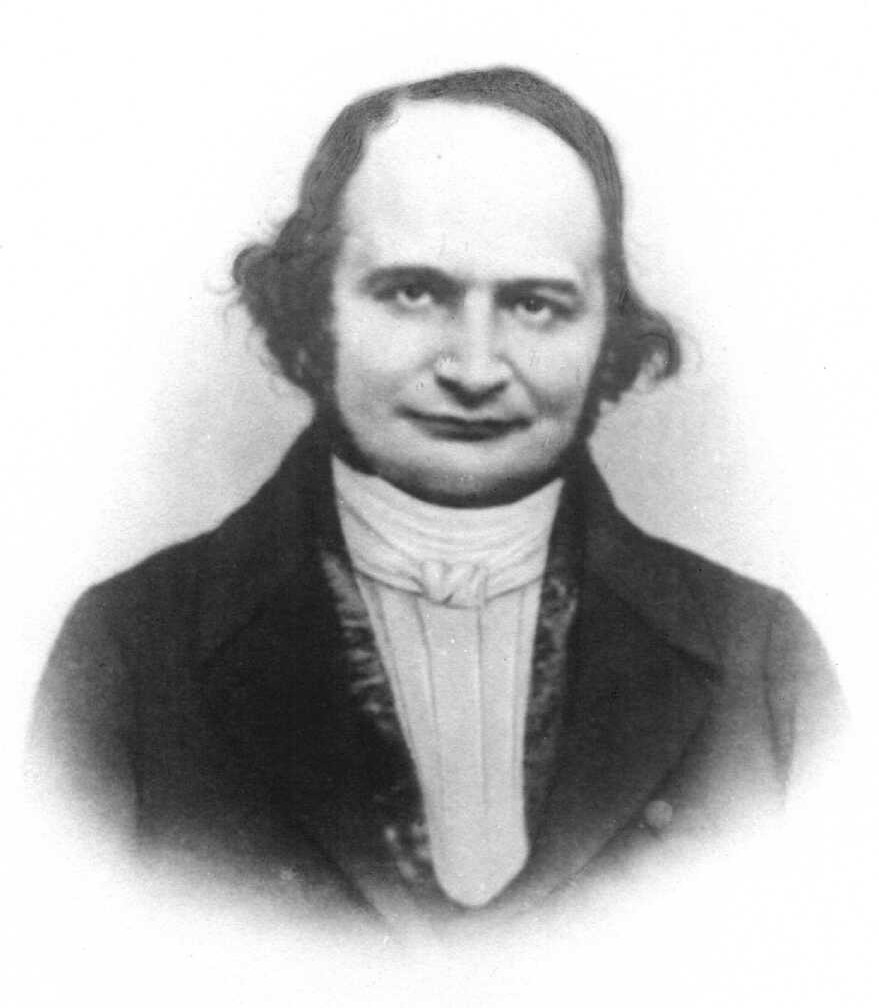
\includegraphics{numeric/figures/c_jacobi}
  \caption{Carl Gustav Jacob Jacobi (1804-1851)}
\end{marginfigure}

Let's return to the discretised version of the Helmholtz equation Eq.~\ref{eq-hh-diff}:

\begin{equation}
f_{i+1} -2 f_i + f_{i-1} + \Delta x^2 k^2 f_i = 0 \label{eq-hh-diff-2}
\end{equation}  

The subscript $i$ denotes the values at position $x_0 + i \Delta x$.

Now, let's start from an initial set of estimates $f_i^0$, where the superscript denotes the iteration number. For Jacobi iteration, the update rule to go from estimates $f_i^n$ to $ f_i^{n+1}$ is defined as

\begin{equation}
f_{i+1}^n -2 f_i^n + f_{i-1}^n + \Delta x^2 k^2 f_i^n = \alpha (f_i^{n+1} - f_i^n ) \label{eq-jacobi}
\end{equation}  

Here, $\alpha$ is by convention a positive real number. Another way of looking at Eq.~\ref{eq-jacobi} is saying that the difference between the old and the new field is proportional to the error (i.e. difference from zero) we get when plugging the old field in Eq.~\ref{eq-hh-diff-2}.

\begin{cue}
Have a look at this equation and try to understand why such an approach could work. What happens in case the method has found the true solution?  
\end{cue}

This can be understood as follows. If the method has converged, then the successive estimates won't change significantly anymore, such that $ f_i^{n+1} \thickapprox f_i^n $. But this means that the right--hand side of Eq.~\ref{eq-jacobi} will be equal to zero, or alternatively that $f_i^n$ is indeed the solution of Eq.~\ref{eq-hh-diff-2}.

The (positive) parameter $\alpha$ is called the relaxation parameter, which can be fine--tuned by the user of the method.

\begin{cue}
What could be advantages/disadvantages of having a small/large value of $\alpha$? 
\end{cue}

A small value of $\alpha$ means that the $f$ values will change rapidly from iteration to iteration, but with the risk of taking such large steps that the method won't converge. On the other hand, a larger value of $\alpha$ reduces the risk of diverging solutions, but on the other hand more iterations will be needed to reach convergence.

To clarify this further, we will now investigate when the Jacobi method diverges, i.e. when the $f$--values become unbounded for a bounded initial estimate.

\subsectionyoutube{Stability analysis of the Jacobi method}{HpHmTQILeCA}

Ideally, we'd like to know under what circumstances this method will converge to the exact solution. However, in this section, we're going to look at an easier subproblem: figuring out when the procedure will diverge, i.e. result in infinite field values. This stability is a necessary step for convergence.\marginnote{Turns out it's also a sufficient criterion, because of something called the Lax equivalence theorem.}

To study divergence, we take an approach that is based on Fourier analysis: the field profile at any iteration can be written as a sum of Fourier components $e^{-j k_x x}$, which are nothing other than plane waves with wavevector $k_x$. Let's take such a plane wave and investigate what happens when iterating through the Jacobi method. If the amplitude of a plane wave stays bounded when iterating, and this is true for all admissible wavevectors $k_x$, then we can be sure that whatever initial estimate will be used, the method will not produce an unbounded result at some time.

Our plane waves take the following form:

\begin{equation}
f_i^n = e^{-j k_x i \Delta x}
\end{equation} 

(Let's not worry about the amplitude, as we will be looking at the ratio $\frac{f_i^{n+1}}{f_i^{n}}$, and the Jacobi procedure is a linear one.)

\begin{cue}
Perform one Jacobi iteration on $f_i^n$, i.e. calculate $f_i^{n+1}$. Use that to calculate the ratio $\frac{f_i^{n+1}}{f_i^{n}}$, which will help us see whether this grows without bounds or not.  
\end{cue}

After one Jacobi iteration, we get:

\begin{align}
 e^{-j k_x (i+1) \Delta x} -2 e^{-j k_x i \Delta x} + 
  e^{-j k_x (i-1) \Delta x} + \Delta x^2 k^2  e^{-j k_x i \Delta x} \\ \nonumber
 = \alpha\left(f_i^{n+1} - e^{-j k_x i \Delta x} \right)
\end{align} 

or

\begin{align}
\alpha f_i^{n+1} -  \alpha e^{-j k_x i \Delta x} = e^{-j k_x i \Delta x}  \left[ e^{-j k_x \Delta x} -2 + e^{+j k_x \Delta x} + \Delta x^2 k^2 \right]
\end{align} 

Thanks to Euler, we can write that

\begin{align}
  \alpha f_i^{n+1}  =  e^{-j k_x i \Delta x}  \left[ \alpha +2 \cos {k_x \Delta x} -2 + \Delta x^2 k^2 \right]
\end{align} 

But $ e^{-j k_x i \Delta x}$ is $f_i^n$, so

\begin{equation}
\frac{f_i^{n+1}}{f_i^{n}} =  1 + \frac{1}{\alpha}\left[2 \cos ( k_x  \Delta x) - 2 + \Delta x^2 k^2\right]
\label{eq-jacobi-conv}
\end{equation} 

(That's actually the main reason we were studying the problem in the Fourier space: plane waves are eigenfunctions of the Helmholtz equation, so we can factor them out in our calculations here.)

\begin{cue}
Derive a criterion for this ratio to remain bounded, irrespective of the choice of a positive value of the relaxation parameter $\alpha$. Pay special attention to the DC plane wave component, i.e. $k_x=0$. 
\end{cue}

Remember that by convention $\alpha$ is positive. In order for Eq.~\ref{eq-jacobi-conv} not to diverge, we should have that $\left|f_i^{n+1} / f_i^{n}\right| \le 1$. \marginnote{This is not sufficient, as $f_i^{n+1} / f_i^{n}$ should also be bigger than -1.}A necessary condition for this, is that the stuff between square brackets is negative. So, at least we need to have that

\begin{equation}
2 \cos ( k_x  \Delta x) - 2 \lt - \Delta x^2 k^2 \label{eq-conv-jacobi}
\end{equation} 

Since the cosine lies between -1 and 1, the left--hand side of this equation lies between -4 and 0 and reaches its maximum for $k_x=0$, which is an important case as it corresponds to a uniform solution. Since it's very likely that the final solution has a DC component, we better make sure that the method converges in this case. However, for this case, we can only satisfy Eq.~\ref{eq-conv-jacobi} if $k=0$. \marginnote{People have tried to address this using a pair of \emph{complex} values for $\alpha$ (J. Comp. Phys. 203, 358–370, 2005).}So, this means that unfortunately the Jacobi method is non--convergent for the general Helmholtz equation, but only works for Laplace's equation, i.e. the special case where $k=0$.

\pagebreak

\sectionyoutubeugent{Finite differences in the time domain}{Pmx2rbBBuOc}
\label{week6}

Without going into any detail, we finally want to mention extremely briefly the existence of a very popular method to solve Maxwell's equations in the time domain. This \textbf{finite--difference time--domain} method (FDTD) uses central differences to discretise the full vectorial Maxwell's equations both in space and time.

It uses a staggered grid, i.e. the electric field and the magnetic field are not discretised at the same point in space, but are arranged in a \textbf{Yee cell} (Fig.~\ref{fig-yee}). The arrangement of the field components in a Yee cell is such that the discretised curl laws of Maxwell's equations can be written out in a natural form.

\begin{figure}
\centering
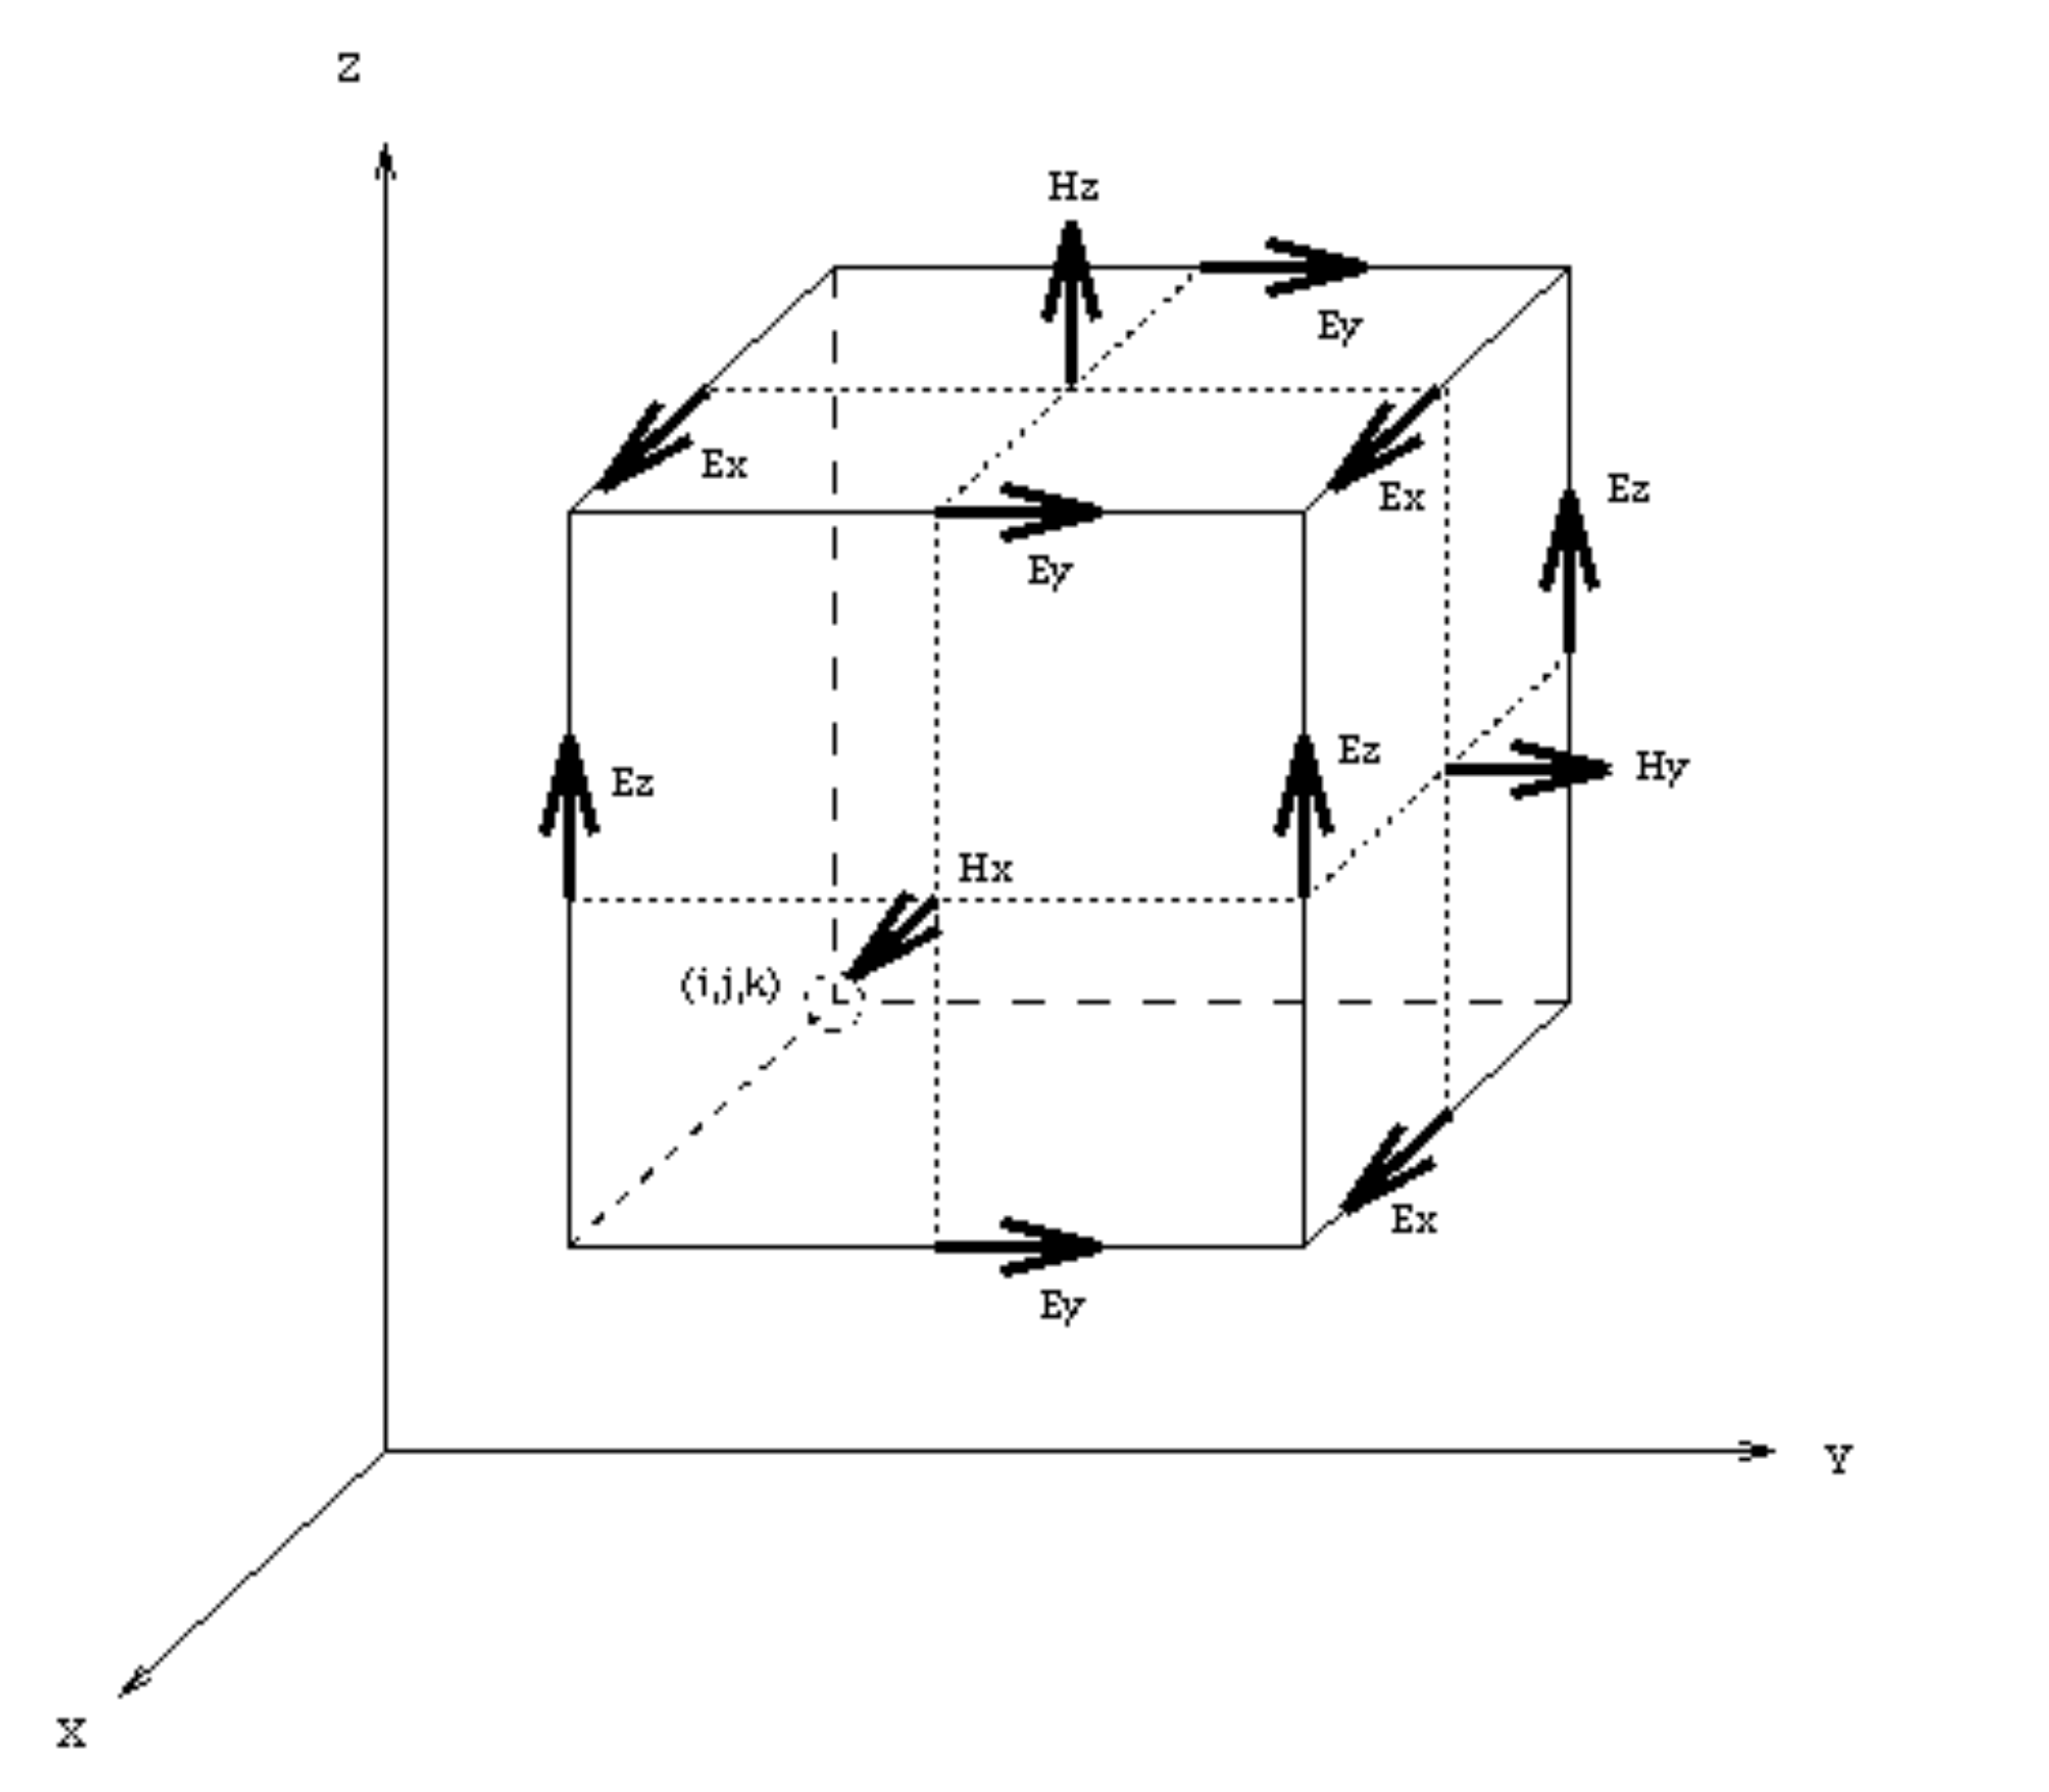
\includegraphics[width=7cm]{numeric/figures/yeecell}
\caption{The Yee cell in the FDTD algorithm.}
\label{fig-yee}
\end{figure}

As for the time evolution of the fields, FDTD uses a leap--frogging scheme, where the electric fields calculated at $t=0$ are used to determine the magnetic fields at $t=0.5$. These are subsequently used to calculate the electric fields at $t=1$ and so on.

Such a brief description obviously glosses over many important points, so consult the literature for more details.

What is important to remember though, is that this is a very general method, but the price you pay for its brute-force character is a large computational cost, combined with intrinsic errors due to the discretisation. So, always do a convergence analysis of your results as a function of the grid size.

\pagebreak

\begin{exer}
% difficulty: normal  
Use Python and its libraries NumPy and SciPy to program a finite-difference method to solve the following differential equation

$$ -\left(a(x) u'(x) \right)' + c(x)u(x) = f(x)$$

in the interval $[0,1]$, with the functions $a$, $a'$, $c$ and $f$ given, and $u(0) = u(1) = 0$. Assume that $a$ and $c$ are positive in the interval of interest.\\

Expand the derivative of the product, and use a backward-difference approximation for $u'$ and a central-difference approximation for $u''$. \\

Use a sparse solver to take advantage of the banded matrix structure. Consult the SciPy documentation for the right way to construct these matrices. \\

To check your results, try the solver using the following set of functions:

$$a_1(x) = 1 + x^2$$
$$c_1(x) = 0$$
$$u_1(x) = x(1-x) e^x $$

To do so, construct the required $f(x)$ from $a_1(x)$, $c_1(x)$ and the exact solution $u_1(x)$ and evaluate how close the numerical approximation of $u$ is to this analytical form.

\end{exer}



\pagebreak


\sectionyoutubeugent{Basic recipe for finite elements}{My6txtzMZHg}

Contrary to e.g. in finite differences, in finite elements we don't solve a differential equation directly, but rather take an oblique approach, as we will see below. All finite element methods more or less share the same philosophy, which is outlined in the following recipe:

\begin{itemize}
\item

\begin{marginfigure}
\centering
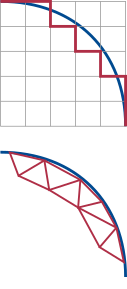
\includegraphics[width=3cm]{numeric/figures/staircase}
\caption{A triangular mesh follows a curved boundary much better than a square grid.}
\label{fig-staircasing}
\end{marginfigure}

\begin{marginfigure}
\centering
\includegraphics[scale=0.5]{numeric/figures/grid}
\caption{A triangular mesh that is locally refined.}
\label{fig-grid}
\end{marginfigure}

Subdivide the structure you want to model into $L$ finite subregions (the "finite elements"). A triangular mesh is a popular choice, because this allows one to approximate curved boundaries much better than e.g. with the rectangular grid that was used in finite difference methods (Fig.~\ref{fig-staircasing}). A second advantage is that all elements don't have to be the same size, so that you can use more elements where a higher resolution is required (Fig.~\ref{fig-grid}). Such a local refinement of the grid turns out to be much more complicated in a finite-difference method.
  
\item
In each separate element $l$, approximate the function $\psi$ you are looking for, using an approximation of the form
\begin{equation}
\psi_l(x,y) = \sum_{i=1}^M u_{i,l} b_{i,l}(x,y) \label{eq-fe-1}
\end{equation}

Here the $b_{i,l}(x,y)$ are some convenient set of known basis functions. In order to solve the problem, the $M$ unknown coefficients $u_{i,l}$ per element $l$ still need to be determined.

\item
Join the different elements, e.g. by ensuring that $\psi$ is continuous across the boundaries between the elements. This introduces some relationship between the $LM$ number of unknowns.


\item
Write down an expression $J$ involving the field in all elements, i.e. containing all the basis functions $b_{i,l}$ and all the expansion coefficients $u_{i,l}$. Because the  $b_{i,l}$ are chosen in advance and therefore known, $J$ is function of the unknown $u_{i,l}$ only. The precise form of $J$ differs from problem to problem, but is often related to the energy in the system.

\item
Find the coefficients $u_{i,l}$ such that $J$ is minimised. In a popular method due to \textbf{Rayleigh and Ritz}, this is done simply by setting all $\partial J / \partial u_{i,l}$ equal to zero and solving the resulting linear system. If $J$ is an expression for the total energy in the system, there is a clear physical interpretation for this procedure: the true solution to the problem is one that minimises the energy in the system.
\end{itemize}


\pagebreak


\sectionugent{Solving the 1D wave equation with finite elements}

\subsectionyoutube{Subdivide the structure}{wBzcZS_XkNo}

In order to make the recipe from the previous section more concrete, we will now indicate in more detail how finite elements can be used to solve the 1D Helmholtz equation in a uniform medium, i.e. the same problem we used to illustrate the concept of finite differences:

\begin{equation}
\frac{d^2 \psi (x)}{d x^2} + k^2 \psi(x) = 0 \label{eq-helmholtz-1d-2}
\end{equation} 

We will subdivide our domain into $L$ finite elements being line segments of identical length.

\subsectionyoutube{Approximate the unknown function}{ZGmyCwsTays}

To describe the unknown function $\psi$ in a certain element $l$, we will use a very simple but common approach, which is that of a piecewise straight approximation.  I.e., in each segment, we will assume that $\psi$ varies linearly between the end points (often called \textbf{nodes} of the mesh) $x_1$ and $x_2$ of that segment:

\noindent\marginnote[1cm]{To see that this is a linear interpolation, just substitute $x$ with $x_1$ and $x_2$ and check what happens.}

\begin{equation}
\psi_l(x) = \frac{x_2 - x}{x_2 - x_1} \psi_1 + \frac{x - x_1}{x_2 - x_1} \psi_2 \label{eq-fe-2}
\end{equation} 

Here $\psi_1$ and $\psi_2$ are the so far unknown values of $\psi$ at $x_1$ and $x_2$ respectively. (To lighten the notation, we omit the index $l$ here, but strictly speaking we should write $x_{1,l}$, $\psi_{2,l}$, etc.)

\begin{cue}
Looking at Eq.~\ref{eq-fe-2}, what would be the set of basis functions we use in this case?
\end{cue}

Comparing Eq.~\ref{eq-fe-1} and \ref{eq-fe-2}, we get that $M=2$, $u_i$ is $\psi_i$ and

\begin{align}
b_1(x) =& \, \frac{x_2 - x}{x_2 - x_1} \\
b_2(x) =& \, \frac{x - x_1}{x_2 - x_1}
\end{align} 

\begin{marginfigure}[-5cm]
\centering
\includegraphics{numeric/figures/interpol}
\caption{Simple shape functions $b_1(x)$ and $b_2(x)$ for a 1D finite element model.}
\label{fig-shape}
\end{marginfigure}

These shape functions or interpolation functions are sketched in Fig.~\ref{fig-shape}.

(It is sometimes useful to express the interpolation functions in terms of a local scaled coordinate $\xi=(x-x_1)/(x_2-x_1)$ ranging from 0 to 1. The advantage of local coordinates is that expressions can be more easily applied to the case where the size of the elements is not the same throughout the mesh.)

\subsectionyoutube{Join the elements}{5GLzU89pYc0}

As mentioned before, the elements are not independent, but are usually coupled through some continuity condition. In the case of our problem, $\psi$ needs to be continuous across elements. The effect of this is that the number of unknowns is reduced.

\begin{marginfigure}[0.5cm]
\centering
\includegraphics{numeric/figures/connect}
\caption{\textbf{Top}: disconnected local numbering. \textbf{Bottom}: connected global numbering.}
\label{fig-connect}
\end{marginfigure}

To see how this is done in practice, consider Fig.~\ref{fig-connect}. Rather than numbering the nodes $\psi_{l,1}$ and $\psi_{l,2}$, let's use a numbering scheme with only a single index. The top of Fig.~\ref{fig-connect} shows a \textbf{disconnected} local numbering scheme, where the two nodes of each element are always given a new number. On the other hand, the bottom of Fig.~\ref{fig-connect} shows a \textbf{connected} global numbering scheme, which already takes the continuity conditions into account. I.e., nodes with a different number in the disconnected scheme but which are physically the same, are merged and only given a single number.

\begin{cue}
For the example in Fig.~\ref{fig-connect}, use a matrix to express the relation between $\psi_{i, \mathrm{disc}}$ in the disconnected numbering scheme and  $\psi_{i, \mathrm{con}}$ in the connected numbering scheme.
\end{cue}
  
The disconnected values are related to connected values by the following matrix equation:

\begin{equation}
\begin{bmatrix}
\psi_1 \\ \psi_2 \\ \psi_3 \\ \psi_4 \\ \psi_5 \\ \psi_6
\end{bmatrix}_{\mathrm{disc}}
=
\begin{bmatrix}
1 & 0 & 0 & 0  \\ 
0 & 1 & 0 & 0  \\   
0 & 1 & 0 & 0  \\ 
0 & 0 & 1 & 0  \\   
0 & 0 & 1 & 0  \\  
0 & 0 & 0 & 1  
\end{bmatrix}
\begin{bmatrix}
\psi_1 \\ \psi_2 \\ \psi_3 \\ \psi_4
\end{bmatrix}_{\mathrm{con}}
\label{eq-con-matrix}
\end{equation} 

The matrix in Eq.~\ref{eq-con-matrix} is called the \textbf{connection matrix} {\mathbf C} of the mesh. Obviously, for such a simple case is seems overkill to write the continuity equations in matrix form, but for complicated 3D meshes such a matrix has its practical value for a computer implementation.

\pagebreak

\subsectionyoutube{Write down an expression for $J$}{vdAuouW_9NY}

In order to keep the method physically interpretable, let's use the electromagnetic energy of the system as an expression for $J$.

From the complex Poynting theorem, we know that the time--averaged stored energy $\mathcal{E}$ in a system is given by (assume our systems are lossless and therefore have real $\varepsilon$ and $\mu$)

\begin{align}
\mathcal{E} =& \, \frac{1}{2} \int \left( {\mathbf E} \cdot {\mathbf D}^* - {\mathbf H} \cdot {\mathbf B}^* \right ) dx \\
  =& \, \frac{1}{2} \int \left( \varepsilon |{\mathbf E}|^2 - \mu |{\mathbf H}|^2 \right) dx
\end{align} 

\begin{cue}
Use Maxwell to eliminate ${\mathbf E}$ from that expression. Then, simplify it for the TM case where ${\mathbf H} = H {\mathbf 1}_z = \psi {\mathbf 1}_z $.  
\end{cue}

To eliminate ${\mathbf E}$, we can use one of Maxwell's curl laws:

\begin{equation}
{\mathbf E} = \frac{1}{j \omega \varepsilon} \nabla \times {\mathbf H}
\end{equation}  

Let's assume that we are working in the TM case, where ${\mathbf H} = H {\mathbf 1}_z = \psi {\mathbf 1}_z $. This means that in our 1D case, $\nabla \times {\mathbf H}=-{\frac{d H}{d x}}{\mathbf 1}_y $, so that we get

\begin{equation}
\mathcal{E} = \frac{1}{2} \int \left( \frac{1}{\omega ^2 \varepsilon}\left|{\frac{d H}{d x}}\right|^2 - \mu |H|^2 \right) dx
\end{equation}

Although we will not prove it here, it can be shown that in the case of lossless media, we can always scale the solution by a complex factor such that the absolute values in the previous equation can be replaced by simple squares.

Remember that we're working in a uniform medium, such that $\varepsilon$ is constant everywhere. That way, to minimise $\mathcal{E}$, we can just as well multiply everything by the constant $2 \omega ^2 \varepsilon$. Therefore, we can define $J$, our quantity to be minimised, as

\begin{equation}
J = \int \left( \left(\frac{d H}{d x}\right)^2 - k^2 H^2 \right) dx
\end{equation}

or, going back to our function $\psi$:

\begin{equation}
\fbox{$\displaystyle
J = \int \left( \left(\frac{d \psi}{d x}\right)^2 - k^2 \psi^2 \right) dx \label{eq-J-power}
$}
\end{equation} 

The exact form of $J$ can now be calculated in terms of the unknown nodal values $\psi_i$, using the explicit form of the shape functions from Eq.~\ref{eq-fe-2}. This is tedious but straightforward, and we will not bother with it here. However, we will just look at the general structure. In view of the linear nature of $\psi$ and the quadratic structure of Eq.~\ref{eq-J-power}, the contribution $J_l$ of a single element $l$ leads to an equation containing squares $\psi_i^2$ and mixed products $\psi_i \psi_j$ of the nodal values. This means we can write it as a bilinear form:

\begin{equation}
J_l = \begin{bmatrix}
\psi_{2l-1} \psi_{2l} 
\end{bmatrix}_\mathrm{disc}
\begin{bmatrix}
A & B \\
C & D 
\end{bmatrix}
\begin{bmatrix}
\psi_{2l-1} \\ \psi_{2l}
\end{bmatrix}_\mathrm{disc}
\label{eq-J-power-i}
\end{equation} 

The elements of the matrix are complicated expressions whose exact value can be determined from evaluating $J$ exactly. To be consistent with the numbering of the nodal values we used before, the index $l$ starts at 1, so that e.g. the nodal elements of the first element are $\psi_{1,\mathrm{disc}}$ and $\psi_{2,\mathrm{disc}}$.

Next up, the total energy $J$ is just the sum of the contributions $J_l$ from all elements. This total energy can also be cast in matrix form, this time with a block diagonal matrix, each block corresponding to a matrix of the type from Eq.~\ref{eq-J-power-i}.

\begin{exer}
  % difficulty: trivial
  % youtube: MLrrcDAmzzg 
Explicitly write down this total energy $J=\sum J_l$ as 

$$J={\mathbf \Psi}^{T}_\mathrm{disc} {\mathbf M} {\mathbf \Psi}_\mathrm{disc}
$$ 

Here, ${\mathbf M}$ is a block diagonal matrix, and ${\mathbf \Psi}_\mathrm{disc}$ is a column vector containing all nodal elements $\psi_i$ in the disconnected numbering scheme.
\end{exer}

Finally, the expressions in terms of disconnected nodal values can be transformed in terms of connected values using the connection matrix ${\mathbf C}$, like e.g. the one from Eq.~\ref{eq-con-matrix}. 

\begin{equation}
J = {\mathbf \Psi}^{T}_\mathrm{con}  {\mathbf C}^T {\mathbf M} {\mathbf C}  {\mathbf \Psi}_\mathrm{con}
\end{equation} 

In this way, all the continuity conditions are imposed.

\pagebreak

\subsectionyoutube{Minimise $J$}{tVEGbGtwvFU}

\begin{marginfigure}[0.5cm]
  % credits: Wikipedia
  % url: https://en.wikipedia.org/wiki/John_William_Strutt,_3rd_Baron_Rayleigh
  \includegraphics{numeric/figures/Rayleigh}
  \caption{John William Strutt, 3rd Baron Rayleigh (1842-1919)}
\end{marginfigure}

To find the unknowns $\psi_{i,\mathrm{con}}$ that minimise $J$, we follow the Rayleigh-Ritz method and simply impose

\begin{equation}
\frac{\partial J}{\partial \psi_{i,\mathrm{con}}} = 0 \label{eq-rayleigh-ritz}
\end{equation} 

and this for all $i$. Remember that $J$ is a bilinear form, containing terms like $\psi_{i,\mathrm{con}}^2$ and $\psi_{i,\mathrm{con}}\psi_{j,\mathrm{con}}$. This means that Eq.~\ref{eq-rayleigh-ritz} takes the form of a set of linear equations, as many as there are unknowns. 

Just as was the case with the finite--difference method, this system can either be solved directly or iteratively.

If you're still uncomfortable that minimising $J$ is mathematically 100\% equivalent to solving the Helmholtz equation, don't worry, as we will show this more rigourously in a future section.

\pagebreak

\sectionyoutubeugent{Finite elements as a variational method}{klAmM-aV9rA}

In theory, the outline of the finite element method that we have given so far is perfectly adequate to describe it. However, it yields additional insight to cast it in the framework of a variational method.

Before doing that, let's recap some well-known facts, but in such a way that will make it easier for us to generalise to the new terminology.

A function $f(x)$ of one variable takes a number $x$ as input, and delivers another number as output. Suppose this function has a minimum for some value of $x$. At that point, the output of the function does not change to first order, i.e. $\delta f=0$ for all possible directions $\delta x$ around that point. Obviously, in this 1D case, there are only two trivial directions, i.e. $+x$ and $-x$.

A function $f(x,y)$ of two variables takes two numbers $x$ and $y$ as input, and spits out another number as output. Also here, when there is a minimum, the output of the function does not change, i.e. $\delta f=0$ for all possible directions  $\delta x \mathbf{1}_x  + \delta y\mathbf{1}_y$ you might explore in the neighbourhood of the minimum.

\begin{marginfigure}[-1.5cm]
  \includegraphics{numeric/figures/function_functional}
  \caption{Function vs. functional}
  \label{fig-function-functional}
\end{marginfigure}

Now, let's introduce a \textbf{functional}. This is an object $F(f(x))$ that consumes as input a function $f(x)$ and delivers a number as output (Fig.~\ref{fig-function-functional}). In contrast to functions, you could say that the input of a functional is not finite dimensional, but infinite dimensional, as it takes an infinite set of numbers to specify an arbitrary function. All of these objects however have a single number as output.

\begin{cue}
Can you think of examples of a functional?  
\end{cue}

The entity $J$ that we have introduced in this chapter is a functional, as it maps a function $\psi$ to a scalar (being in this case the energy of the system), so $\mathcal{E}=J(\psi)$.

\begin{exer}
  % difficulty: trivial
  % ugent
  % youtube: gbKEmkNIA6k
  Function or functional?

  a) $f(x)=\int_0^x t^2 dt$

  b) $f(x)=\int_0^1 x^2(t) dt$
  \begin{sol}
    a) function b) functional
  \end{sol}
\end{exer}

A \textbf{variational expression} comes from minimising a functional over a set of admissible functions. Indeed, every input $\psi$ to the functional will result in a different number $J(\psi)$ at the output, and we are looking for the special $\psi$ that will result in the smallest possible output.

In the case of finite elements, we have been solving the following variational expression:

\begin{equation}
\mathcal{E} = \min_\psi J(\psi)
\end{equation} 

where $\mathcal{E}$, is the total energy in the system, and $\psi$ are functions coming from an admissible set, e.g. continuous functions that satisfy the boundary conditions of the problem.

\begin{marginfigure}[-1.5cm]
  % credits: Wikipedia
  % url: https://en.wikipedia.org/wiki/Walther_Ritz
  \includegraphics{numeric/figures/w_ritz}
  \caption{Walther Ritz (1878-1909)}
\end{marginfigure}

The \textbf{Rayleigh--Ritz} method to minimise a functional is to expand $\psi$ in a finite number of known basis functions, and then determine the expansion coefficients such that the functional is minimised. This turns the infinite-dimensional problem into a much more tractable finite-dimensional one. (Nitpicking: this effectively turns the functional $J(\psi)$ into a vanilla function $J(\psi(\psi_i))$, albeit one of multiple arguments.)

\begin{cue}
What can you say about the sensitivity of $\mathcal{E}$, to e.g. rounding errors, given that we are working at the minimum of the functional? 
\end{cue}

\begin{marginfigure}[1.5cm]
  \includegraphics{numeric/figures/minimum}
  \caption{A function (or functional) does not vary to first order at its minimum.}
  \label{fig-functional-min}
\end{marginfigure}

So far, we don't seem to have done anything useful except introducing some new terminology. However, by looking at the energy $\mathcal{E}$, as a minimum of a functional, we realise that a small variation $\delta \psi$ (caused e.g. by numerical round--off errors) will not have a very big impact on the calculated value of $\mathcal{E}$, since $\delta J=0$ at the minimum of the functional, for all possible 'directions' $\delta \psi$. This insensitivity to errors is a big bonus for practical applications, and means that methods which have a variational basis can be much more robust.

Now, the energy $\mathcal{E}$ is a decidedly uninteresting quantity for practical applications, so the fact that we can calculate it without being very sensitive to rounding errors is of limited use. However, it is possible to derive variational expressions for e.g. the propagation constant of a waveguide, which is a much more relevant parameter that people are interested in.

\pagebreak


\sectionyoutubeugent{Variational form for the 3D Helmholtz equation}{vORxFwwLm6c}

In this section, we wish to provide some extra proof that a function that minimises the functional from Eq.~\ref{eq-J-power} is indeed a solution to the Helmholtz equation. So far, this was only made acceptable by invoking physical arguments based on minimum energy, but a mathematical proof for this was lacking. At the same time, let's extend the method to three dimensions:

\begin{equation}
J = \iiint \left((\nabla \psi)^2 - k^2 \psi^2 \right) dV \label{eq-variational1}
\end{equation} 

\noindent\marginnote{$\delta J=0$ can obviously also give us a maximum, but these situations are rare in practice and can be easily identified by exploring $J$ in the neighbourhood of the potential solution.}If a function $\psi$ minimises the functional $J$, then $\delta J$ has to be zero for $\psi$.

\begin{cue}
Calculate $\delta J = J(\psi + \delta \psi) - J(\psi)$ for this functional, neglecting second-order terms in $\delta \psi$.
\end{cue}

\noindent\marginnote[3.3cm]{Don't get confused: $\left( \nabla \psi \right)^2 = \nabla \psi \cdot \nabla \psi \ne \nabla^2 \psi = \nabla \cdot \nabla \psi$}For $\delta J$ (also called the \textbf{first variation} of $J$) we get

\begin{align}
\delta J =& \, J(\psi + \delta \psi) - J(\psi) \nonumber \\
  =& \, \iiint \left( (\nabla (\psi + \delta \psi))^2 - k^2 (\psi + \delta \psi)^2 \right) dV \nonumber   \\
  -& \, \iiint \left((\nabla \psi)^2 - k^2 \psi^2 \right) dV
\end{align} 

If we neglect second-order terms in $\delta \psi$, we get

\begin{equation}
\delta J = \iiint \left( 2 \nabla \psi \cdot \nabla (\delta \psi) - 2 k^2 \psi \delta \psi \right) dV \label{eq-var-helmholtz-1}
\end{equation}

Now, let's make use of the following vector identity:

\begin{equation}
\nabla \cdot (u \nabla v) = u \nabla \cdot \nabla v + (\nabla u) \cdot (\nabla v) \label{eq-vector-id-green-other}
\end{equation} 

\noindent\marginnote[-1.8cm]{To flex your vector calculus muscles, you can easily verify that all three terms turn out to be scalars.}

\begin{cue}
Take the volume integral of this identity and apply the divergence theorem. Next, use this expression to transform $\delta J$. Figure out how to best assign $u$, $v$ to $\psi$, $\delta \psi$, bearing in mind that the ultimate goal is to bring out the Helmholtz equation.
\end{cue}

Since the Helmholtz equation contains $\nabla^2 \psi = \nabla \cdot \nabla \psi$, let's assign $v$ to $\psi$ and $u$ to $\delta \psi$, as that will bring us closer to the Helmholtz equation. Additionally, this will result in a term that figures in Eq~\ref{eq-var-helmholtz-1}. By integrating Eq.~\ref{eq-vector-id-green-other}, we get

\begin{equation}
  \iiint  \nabla \cdot (\delta \psi \nabla \psi) dV =  \iiint \delta \psi  \nabla^2 \psi dV + 
  \iiint  \nabla (\delta \psi) \cdot \nabla \psi  dV  
\end{equation} 

Using the divergence theorem and bringing the final term, i.e. the term from Eq~\ref{eq-var-helmholtz-1}, to the left-hand side, we get

\begin{equation}
\iiint \nabla \psi \cdot \nabla (\delta \psi) dV = \iint \delta \psi {\nabla \psi} \cdot \mathbf{1}_n dS - \iiint \delta \psi \nabla^2 \psi dV
\end{equation} 

Here, $\mathbf{1}_n$ is the unit vector perpendicular to the surface, and ${\nabla \psi} \cdot \mathbf{1}_n $ is by definition equal to the normal derivative ${\partial \psi} / {\partial n}$. This means that

\begin{equation}
  \iiint \nabla \psi \cdot \nabla (\delta \psi) dV = \iint \delta \psi  \frac{\partial \psi}{\partial n} dS - \iiint \delta \psi \nabla^2 \psi dV
  \end{equation} 

\noindent\marginnote[-1.5cm]{This is actually one of the many incarnations of Green's theorem.}

\begin{cue}
Use this result in $\delta J$, and impose the condition that says that $\psi$ should minimise $J$.  
\end{cue}

Using this in the expression for $\delta J$, we get

\begin{equation}
\delta J = 2\iint \delta \psi  \frac{\partial \psi}{\partial n} dS - 2\iiint \delta \psi  \nabla^2 \psi dV - 2 \iiint k^2 \psi \delta \psi dV
\end{equation} 

Demanding that $\delta J = 0$ (a condition which is called \textbf{stationarity}), we get

\begin{equation}
\iiint \delta \psi (\nabla^2 \psi + k^2 \psi ) dV = \iint \delta \psi  \frac{\partial \psi}{\partial n} dS \label{eq-euler-lagrange-1}
\end{equation}

\begin{cue}
Think about how to deal with the term involving the boundary conditions, i.e. the 2D integral.  
\end{cue}

\pagebreak

\begin{marginfigure}[0.2cm]
  % credits: Wikipedia
  % url: https://en.wikipedia.org/wiki/Peter_Gustav_Lejeune_Dirichlet
  \includegraphics{numeric/figures/p_dirichlet}
  \caption{Peter Gustav Lejeune Dirichlet (1805-1859)}
\end{marginfigure}

Suppose that our boundary conditions are of the Dirichlet type such that $\psi=0$ on the boundary. In other words, we are restricting our search to only include functions that vanish at the boundary. Then, in order to be an admissible function that satisfies the boundary condition, $\delta \psi$ also has to be zero on the boundary, so that the right--hand side of Eq.~\ref{eq-euler-lagrange-1} will be zero.

Similarly, for Neumann--type boundary conditions where $\partial \psi / \partial n = 0$ on the boundary, the right--hand side of Eq.~\ref{eq-euler-lagrange-1} will also be zero.

So, for these common boundary conditions, we get that demanding that $\delta J = 0$ results in

\begin{equation}
\iiint \delta \psi (\nabla^2 \psi + k^2 \psi ) dV = 0
\end{equation} 

To minimise $J$, $\delta J$ should be zero not just for a particular lucky choice of $\delta \psi$, but it should actually be zero for any choice of $\delta \psi$. So, stationarity of the variational expression requires that $\psi$ has to satisfy

\begin{equation}
\nabla^2 \psi + k^2 \psi = 0 \label{eq-euler-lagrange-2}
\end{equation} 

This is of course the Helmholtz equation.

Eq.~\ref{eq-euler-lagrange-2} is called the \textbf{Euler} or the \textbf{Euler--Lagrange} equation of the variational formulation Eq.~\ref{eq-variational1}. So, rather than finding a function which minimises a certain functional in a variational formulation, we can explicitly solve a partial differential equation and achieve the same thing.

Other bits of terminology: a variational formulation of a problem is sometimes called a \emph{weak formulation}, whereas the corresponding differential equation is the \emph{strong formulation} of that problem.

\pagebreak

\begin{exer}
% difficulty: trivial
% ugent
% youtube: qM9NOykRESw
Show that demanding that the 1D Helmholtz equation is orthogonal to any arbitrary function leads to the variational form 

$$J = \int \left( \left(\frac{d \psi}{d x}\right)^2 - k^2 \psi^2 \right) dx$$

\end{exer}


\begin{exer}
  % difficulty: normal
  % youtube: 7Y6LC9GMrO8
  
Construct the best least-squares approximation to the parabola 

$$f(x) = 10(x-1)^2 -1$$ 

in the entire interval $[1,2]$ using only functions from $V = \mathrm{span} \{1, x\}$.

\begin{sol}
$$-\frac{38}{3} + 10x$$   
\end{sol}
\end{exer}


\begin{exer}
  % difficulty: normal
  % youtube: cwMI8XAVfCQ 
Use the identity

$$\iint_S p \nabla q \cdot \nabla r dS= - \iint_S q \nabla \cdot (p \nabla r) dS + \int_{\delta S} pq \frac{\partial r}{\partial n} dl$$

to find the Euler-Lagrange equation of the following variational expression

$$J(\phi)=\iint_S f(x,y) (\nabla \phi)^2 dS$$

with $f(x,y)$ a given scalar function.

\begin{sol}
$$\nabla \cdot \left( f \nabla \phi \right) = 0 $$
\end{sol}
\end{exer}

% Sorry Leonard, no space here.

%\begin{marginfigure}[3.0cm]
  % credits: Wikipedia
  % url: https://en.wikipedia.org/wiki/Leonhard_Euler
%  \includegraphics{numeric/figures/l_euler}
%  \caption{Leonhard Euler (1707-1783)}
%\end{marginfigure}

\begin{marginfigure}[-5.7cm]
  % credits: Wikipedia
  % url: https://en.wikipedia.org/wiki/Joseph-Louis_Lagrange 
  \includegraphics{numeric/figures/j_lagrange}
  \caption{Joseph-Louis Lagrange (1736-1813)}
\end{marginfigure}

\pagebreak

\begin{exer}
% difficulty: normal
% ugent
% youtube: cHTTlU_ewds
  
  Consider an arbitrarily shaped waveguide filled with air but bounded by perfectly conducting metal walls.

  a) Show that the eigenmodes of the waveguide, i.e. solutions which have a $z$-dependence of $\exp{(-j k_z z)}$, satisfy the following equation:

$$ \nabla_{xy}^2 \psi + \left( k^2 - k_z^2 \right)\psi = 0 $$ 

Here, $\nabla_{xy}$ is the transverse differential operator, which does not contain derivatives in the $z$-direction.

\noindent\marginnote{Note the difference between this cut-off condition for closed metal wave-guides and the one for open wave-guides, which is $k=k_{\mathrm{clad}}$} b) We are interested in finding the value of $k$ at cut--off ($k_z^2=0$), because we can get the cut-off wavelength from that. Show that the following is a variational expression for this cut--off wavevector $k_{\mathrm{cut}}$:

$$ k_{\mathrm{cut}}^2 = \frac{\iint_S (\nabla_{xy} \psi)^2 dS}{\iint_S \psi^2 dS}$$

Here $S$ is the cross--section of the waveguide.

c) Looking back at Eq.~\ref{eq-variational1}, what can you say about the energy of such a mode at cut-off?

\end{exer}


\pagebreak


\sectionugent{Eigenmode expansion}
\label{week7}

\subsectionyoutube{Introduction}{f2M9tZ8461o}

In this section, we'll discuss a method that is not as general as finite difference or finite element methods, but which, for a certain class of structures, can give an important speed boost because it exploits the properties of the structure to be modelled in a natural way.

In the so-called eigenmode expansion method, we are studying structures that consist of a number of layers where the refractive index profile does not change in the propagation direction (often taken to be the $z$--direction). \marginnote{If you're really desperate, you can even take a curved structure, and approximate it by slicing it up in a number of uniform layers, although in that case, you will suffer from staircasing.}This means that the structures are in essence a stack of waveguides, e.g. a Bragg reflector, or any structure that is like a layered cake. 
The simplest case is given in Fig.~\ref{fig-interface}, which shows the interface between two waveguides I and II. This is the building block of more complicated structures.

\begin{figure}[ht]
\centering
\includegraphics{numeric/figures/interface}
\caption{Interface between two layers.}
\label{fig-interface}
\end{figure}

We will expand the field in each waveguide using a basis set that incorporates already a lot of physics of the problem, namely the eigenmodes of that waveguide. It can be shown that these eigenmodes form a \textbf{complete} set, i.e. they can be used to expand any arbitrary field in that layer. Also, by enclosing the structure that we want to model in a metal box, this set of eigenmodes is a discrete set rather than a continuum.

The interface is placed at $z=0$ and a single mode with index $p$ is incident from medium I. This incident mode will give rise to a backward--propagating field in medium I, which we expand in terms of the eigenmodes of this medium. Likewise, we expand the transmitted field in the eigenmodes of medium II.

Before continuing, we need to determine a relationship between the fields of the forward and the backward propagating modes.

\begin{exer}
  % difficulty: trivial
  % youtube: W2p1YCQ6Ra0
Assume you solve Maxwell's equations to find a certain eigenmode solution, i.e. a solution with a $z$-dependence of $\exp{(-j \beta z)}$. Let's say this solution is characterised by the following tangential ($x$ and $y$) and normal ($z$) components:

$$\left( \mathbf{E}_{t},\mathbf{E}_{z},\mathbf{H}_{t},\mathbf{H}_{z},\beta \right)$$

By writing down the different components of Maxwell's curl equations, show that there also exists another solution:

$$  \left( \mathbf{E}_{t},-\mathbf{E}_{z},-\mathbf{H}_{t},\mathbf{H}_{z},-\beta \right) $$

Because of the negative propagation constant, this is the backward propagating version of the same eigenmode.

\end{exer}

\pagebreak

\subsectionyoutube{Mode matching}{q2mp-Y9VDxY}

Now that we've laid the groundwork, we can start applying the so-called \textbf{mode--matching} technique to the interface:

\begin{cue}
Impose the continuity of the tangential components of the total field on both sides of the interface in Fig.~\ref{fig-interface}.  
\end{cue}

Demanding continuity leads to: \marginnote[1.3cm]{Note that the expansion coefficients for $\mathbf{E}$ are the same as those for $\mathbf{H}$. This makes sense, because we're expanding in eigenmodes, and scaling each eigenmode will result in scaling both $\mathbf{E}$ and $\mathbf{H}$ with the same factor.} 

\begin{eqnarray}
\mathbf{E}^{I}_{p,t}+\sum _{j}R_{j,p}\mathbf{E}^{I}_{j,t} & = & \sum _{j}T_{j,p}\mathbf{E}^{II}_{j,t}\label{Eq:MM 1a} \\
\mathbf{H}^{I}_{p,t}-\sum _{j}R_{j,p}\mathbf{H}^{I}_{j,t} & = & \sum _{j}T_{j,p}\mathbf{H}^{II}_{j,t}\label{Eq:MM 1b} 
\end{eqnarray}

(The minus sign for the reflected tangential ${\mathbf H}$ field comes from the explicit form of the backward eigenmode we derived above.)

To calculate the unknown expansion coefficients $R_{j,p}$ and $T_{j,p}$ (which can be seen as reflection and transmission coefficients), we take the right cross product of Eq.~\ref{Eq:MM 1a} with $\mathbf{H}^{I}_{i,t}$ and the left cross product of Eq.~\ref{Eq:MM 1b} with $\mathbf{E}^{I}_{i,t}$. Here, $i$ is an arbitrary index. Afterwards, we integrate over the cross--section.

\begin{cue}
  Perform these operations.
\end{cue}

We get:

\begin{eqnarray}
\left\langle \mathbf{E}^{I}_{p},\mathbf{H}^{I}_{i}\right\rangle +\sum _{j}R_{j,p}\left\langle \mathbf{E}^{I}_{j},\mathbf{H}^{I}_{i}\right\rangle  & = & \sum _{j}T_{j,p}\left\langle \mathbf{E}^{II}_{j},\mathbf{H}^{I}_{i}\right\rangle \label{Eq:MM 2a} \\
\left\langle \mathbf{E}^{I}_{i},\mathbf{H}^{I}_{p}\right\rangle -\sum _{j}R_{j,p}\left\langle \mathbf{E}^{I}_{i},\mathbf{H}^{I}_{j}\right\rangle  & = & \sum _{j}T_{j,p}\left\langle \mathbf{E}^{I}_{i},\mathbf{H}^{II}_{j}\right\rangle \label{Eq:MM 2b} 
\end{eqnarray}

\noindent\marginnote{You can easily verify that in that definition, only the tangential components contribute to the integral.}where the scalar product is defined as the following overlap integral:

\begin{equation} 
\left\langle \mathbf{E}_{m},\mathbf{H}_{n}\right\rangle \equiv \iint _{s}\left( \mathbf{E}_{m}\times \mathbf{H}_{n}\right) \cdot d{\mathbf S}
\end{equation} 

If we decide to truncate the series expansion after $N$ terms, we have $2N$ unknowns: $N$ reflection coefficients and $N$ transmission coefficients. Eq.~\ref{Eq:MM 2a} and \ref{Eq:MM 2b} provide us exactly with $2N$ equations, since we can write them for all $i$ in $1 \cdots N$.

\subsectionyoutube{Exploiting orthogonality}{JdX-Ev-JK2I}

It's possible to show that eigenmodes in a waveguide satisfy the following orthogonality condition ($m \ne n$):

$$\iint_{S}\left( \mathbf{E}_{m}\times \mathbf{H}_{n}\right) \cdot d{\mathbf S}=0$$

\begin{cue}
Reduce the dimensionality of the linear system from the previous section by invoking this orthogonality relation, followed by adding and subtracting the resulting equations.
\end{cue}

The orthogonality condition leads to
  
\begin{eqnarray}
\delta _{ip}\left\langle \mathbf{E}^{I}_{p},\mathbf{H}^{I}_{p}\right\rangle +R_{i,p}\left\langle \mathbf{E}^{I}_{i},\mathbf{H}^{I}_{i}\right\rangle  & = & \sum _{j}T_{j,p}\left\langle \mathbf{E}^{II}_{j},\mathbf{H}^{I}_{i}\right\rangle \label{Eq:MM 3a} \\
\delta _{ip}\left\langle \mathbf{E}^{I}_{p},\mathbf{H}^{I}_{p}\right\rangle -R_{i,p}\left\langle \mathbf{E}^{I}_{i},\mathbf{H}^{I}_{i}\right\rangle  & = & \sum _{j}T_{j,p}\left\langle \mathbf{E}^{I}_{i},\mathbf{H}^{II}_{j}\right\rangle \label{Eq:MM 3b} 
\end{eqnarray}

Adding and subtracting these equations yields

\begin{eqnarray}
\sum _{j}\left[ \left\langle \mathbf{E}^{I}_{i},\mathbf{H}^{II}_{j}\right\rangle +\left\langle \mathbf{E}^{II}_{j},\mathbf{H}^{I}_{i}\right\rangle \right] T_{j,p}=2\delta _{ip}\left\langle \mathbf{E}^{I}_{p},\mathbf{H}^{I}_{p}\right\rangle  &  & \label{Eq:MM 4a} \\
R_{i,p}=\frac{1}{2\left\langle \mathbf{E}^{I}_{i},\mathbf{H}^{I}_{i}\right\rangle }\sum _{j}\left[ \left\langle \mathbf{E}^{II}_{j},\mathbf{H}^{I}_{i}\right\rangle -\left\langle \mathbf{E}^{I}_{i},\mathbf{H}^{II}_{j}\right\rangle \right] T_{j,p} &  & \label{Eq:MM 4b} 
\end{eqnarray}

This shows that we can first calculate the transmission coefficients by solving an $N \times N$ linear system, and then obtain the reflection coefficients by a simple matrix multiplication. This is much more efficient than solving the $2N \times 2N$ system from the previous section for the reflection and transmission coefficients simultaneously.

After obtaining $R$ and $T$ upon incidence of mode $p$, we can of course repeat the whole procedure using all modes $p$ in $ 1 \cdots N$.

\noindent\marginnote{Actually, when solving the system even an explicit inverse is not required, as we can use the LU decomposition of the system matrix.}Important to note is that this changes only the right--hand side in the linear system in Eq.~\ref{Eq:MM 4a}, so that we do not have to invert another system matrix. 

In what follows, we will also choose to normalise our modes such that \( \left\langle \mathbf{E}^{I}_{i},\mathbf{H}^{I}_{i}\right\rangle =1 \), which further simplifies the equations.

\pagebreak

\subsectionyoutube{Overlap matrices}{pdeceZHUlOU}

Let's now define the following overlap matrices:

\begin{eqnarray}
\mathbf{O}_{I,II}\left( i,j\right)  & \equiv  & \left\langle \mathbf{E}^{I}_{i},\mathbf{H}^{II}_{j}\right\rangle \label{Eq:O_I_II} \\
\mathbf{O}_{II,I}\left( i,j\right)  & \equiv  & \left\langle \mathbf{E}^{II}_{i},\mathbf{H}^{I}_{j}\right\rangle \label{Eq:O_II_I} 
\end{eqnarray}

\begin{cue}
Use these matrices to write Eq.~\ref{Eq:MM 4a} and \ref{Eq:MM 4b} more compactly.   
\end{cue}

With the superscript $T$ denoting transpose, we finally get\marginnote{If you need more details here, watch the video.}:

\begin{eqnarray}
\mathbf{T}_{I,II} & = & 2\left( \mathbf{O}_{I,II}+\mathbf{O}^{T}_{II,I}\right) ^{-1}\label{Eq:MM 5a} \\
\mathbf{R}_{I,II} & = & \frac{1}{2}\left( \mathbf{O}^{T}_{II,I}-\mathbf{O}_{I,II}\right)  \mathbf{T}_{I,II}\label{Eq:MM 5b} 
\end{eqnarray}

In these expressions $\mathbf{T}_{I,II}$ and $\mathbf{R}_{I,II}$ are the so--called transmission and reflection matrices. Their \( p \)--th columns consist of the $T_{j,p}$ and $R_{j,p}$ from Eq.~\ref{Eq:MM 4a} and \ref{Eq:MM 4b}. 

If we collect the expansion coefficients of an arbitrary incident field in a column vector $\mathbf{A}_\mathrm{inc}$, we can write very compactly for the reflected and transmitted fields, using the meaning of the $R_{i,j}$ and $T_{i,j}$ coefficients: 

\begin{eqnarray}
\mathbf{A}_\textrm{refl} & = & \mathbf{R}_{I,II} \mathbf{A}_\textrm{inc}\label{Eq:R matrix} \\
\mathbf{A}_\textrm{trans} & = & \mathbf{T}_{I,II} \mathbf{A}_\textrm{inc}\label{Eq:T matrix} 
\end{eqnarray}

Obviously, we can repeat the entire procedure for incidence from medium II, which gives us the matrices $\mathbf{R}_{II,I}$ and $\mathbf{T}_{II,I}$.

These four matrices completely characterise the scattering that occurs at an interface.

\begin{cue}
Study the structure of Eq.~\ref{Eq:MM 5a} and \ref{Eq:MM 5b}. Do they remind you of something?  
\end{cue}

\begin{marginfigure}[-5.0cm]
  % credits: Wikipedia
  % url: https://en.wikipedia.org/wiki/Augustin-Jean_Fresnel
  \includegraphics{numeric/figures/a_fresnel}
  \caption{Augustin-Jean Fresnel (1788-1827)}
\end{marginfigure}

Finally, we want to point out the similarity in structure between Eq.~\ref{Eq:MM 5a} and \ref{Eq:MM 5b} and the well--known Fresnel equations to calculate reflection and transmission for normal incidence of a plane wave upon the interface between two semi--infinite media:

\begin{eqnarray}
T & = & \frac{2n_{1}}{n_{1}+n_{2}}\label{Eq:T normal} \\
R & = & \frac{n_{1}-n_{2}}{n_{1}+n_{2}}\label{Eq:R normal} 
\end{eqnarray}

In fact, Eq.~\ref{Eq:T normal} and \ref{Eq:R normal} can also be derived from the more general treatment presented here. For homogeneous layers, where the refractive index does not vary in the transverse direction, it turns out that the overlap matrices are diagonal, meaning that there is no cross--coupling between the different modes. Further evaluation of the formulas can reveal that the Fresnel equations are indeed recovered.

Obviously, a realistic structure will consist of more than one interface, but that problem is outside the scope of this text.


\begin{exer}
  % difficulty: hard
  % youtube: 6fDVdWvl09c
Derive the matrix form for the eigenmode expansion equations for the reflection and the transmission matrix at an interface, in case the basis functions are not orthogonal. Write them using a block matrix involving the overlap matrices.

\begin{sol}
$$ \begin{bmatrix} \mathbf{O}^{T}_{II,I} & -\mathbf{O}^{T}_{I,I} \\ \mathbf{O}_{I,II} & \mathbf{O}_{I,I} \end{bmatrix} \begin{bmatrix} \mathbf{T}_{I,II} \\ \mathbf{R}_{I,II} \end{bmatrix} =  \begin{bmatrix} \mathbf{O}^{T}_{I,I} \\ \mathbf{O}_{I,I} \end{bmatrix} $$
\end{sol}

\end{exer}


\pagebreak


\sectionugent{Method of weighted residuals}

To conclude this chapter, we will present the method of weighted residuals, a very general scheme for converting linear differential and integral equations into a form suitable for numerical solution by standard matrix methods.

\subsectionyoutube{Working with an error residual}{hdMlNCC6H8s}

We start from a problem of the type

\begin{equation}
L u = v \label{eq-operator}
\end{equation}

where $v$ represents some known excitation and $u$ is the unknown and wanted field. $L$ is a linear operator involving differentiation, integration or both.

\begin{cue}
Cast the Helmholtz equation in this form.  
\end{cue}

For the Helmholtz equation, $v=0$ and $L=\nabla^2 + k^2$. 

Suppose we approximate the unknown $u$ by

\begin{equation}
\tilde{u}(x) = \sum_{i=1}^N u_i b_i(x) \label{eq-expansion}
\end{equation} 

where $b_i(x)$ are a complete set of known basis functions. The general problem is now to choose the coefficients $u_i$ to approximate as well as possible the unknown solution $u$ to Eq.~\ref{eq-operator} with a \emph{finite} number $N$ of basis functions.

\begin{cue}
How would you quantify 'as well as possible'? Is the method you propose useful in practice?  
\end{cue}

Your first hunch could be to try and minimise the difference between the exact solution $u$ and its approximation $\tilde{u}$. However, this will get you nowhere in practice: you don't know the exact solution, so you cannot evaluate the difference.

\begin{cue}
What happens if you apply $L$ to the difference between $\tilde{u}$ and $u$? 
\end{cue}

Doing this, leads to the definition of the \textbf{error residual}:

\begin{equation}
R(x) = L\tilde{u} - Lu = L\tilde{u} - v = L \left( \sum_{i=1}^N u_i b_i(x) \right) - v(x)
\end{equation} 

which is clearly zero if and only if we have an exact solution to Eq.~\ref{eq-operator}. Moreover, apart from the coefficients $u_i$, all the other quantities can be calculated. Now we have a realistic objective: trying to make the residual as small as possible.

\begin{cue}
Think about how you would quantify and minimise the size of this residual. 
\end{cue}

There are many approaches you could take here, e.g. asking that the energy of the residual is minimised, or imposing that the residual vanishes at a set of predefined points.

Here however, we will introduce a more general approach, of which the examples listed above are special cases.

\noindent\marginnote{Don't confuse the weight functions $w_i$ with the weight function you could choose to define your scalar product, e.g. $r$ in the scalar product of Bessel functions. These are completely independent choices.}To proceed, we choose another set of functions, the so--called \textbf{test} or \textbf{weight} functions $w_j$. We also introduce an inner product (scalar product) formally written as $\langle f(x),g(x) \rangle$. The definition of the inner product is in a sense arbitrary and often follows from the specifics of the problem considered.

Rather than asking the impossible that $R(x)=0$ for all $x$, we insist that the residual be orthogonal to each of the weight functions under the scalar product considered (hence the name of the method).

\begin{cue}
Impose this condition and put it in matrix form.  
\end{cue}

This results in the following $N$ equations for $N$ unknowns:

\begin{equation}
\left\langle  L \left(\sum_{i=1}^N u_i b_i(x)\right) - v(x) , w_j(x) \right\rangle = 0 \hspace{0.5cm} j=1,2\cdots,N \label{eq-weighted-res}
\end{equation}

In the above equation, $b_i(x)$, $v(x)$ and $w_j(x)$ are known functions of $x$. $L$ is the known operator and $u_i$ are the unknown and wanted scalars which when put into Eq.~\ref{eq-expansion} give our approximate solution.

Let's move the excitation part to the right-hand side, and exploit the linearity of $L$ to write Eq.~\ref{eq-weighted-res} as

\begin{equation}
  \left\langle  \sum_{i=1}^N u_i L b_i(x), w_j(x) \right\rangle = \left\langle v(x), w_j(x)\right\rangle 
\end{equation}

Of course, the scalar product is linear as well:

\begin{equation}
   \sum_{i=1}^N u_i \left\langle L b_i(x), w_j(x) \right\rangle = \left\langle v(x), w_j(x)\right\rangle  \label{eq-weighted-res-3}
\end{equation}

This can also be put into a compact matrix form:

\begin{equation}
{\mathbf L} {\mathbf u} = {\mathbf v}
\end{equation} 

Here, $\mathbf u$ denotes the unknown column vector containing $u_1, u_2, \hdots, u_N$. $\mathbf v$ denotes the column vector with elements $\left\langle v(x), w_j(x) \right\rangle$. Finally, ${\mathbf L}$ is a  $N \times N$ matrix with $(i,j)$-th element $\left\langle L b_j(x), w_i(x) \right\rangle$. $\mathbf v$ and ${\mathbf L}$ are known, because we can evaluate them based on our choice of basis and test functions.

So, our equation $Lu=v$ has been \emph{projected} by approximation into the matrix equation ${\mathbf L} {\mathbf u} = {\mathbf v}$, which can be solved with standard numerical routines.

Apart from the weighted residuals method, the above procedure is also called the \textbf{method of moments} or the \textbf{generalised Galerkin method}.

\pagebreak

\subsectionyoutube{Choice of basis and test functions}{yzLwNFePkhk}

\begin{marginfigure}[-.0cm]
  % credits: Wikipedia
  % url:  https://en.wikipedia.org/wiki/Boris_Galerkin
  \includegraphics{numeric/figures/b_galerkin}
  \caption{Boris Grigoryevich Galerkin (1871-1945)}
\end{marginfigure}

Starting from the general procedure outlined above, different numerical methods can be derived that are catalogued according to their choice of basis and test functions.

If basis and test functions are chosen equal, i.e. $b_i(x) = w_i(x)$, the method is called the (non--generalised) \textbf{Galerkin method}. Often this leads to a formulation which can be cast in a variational form, having the advantages already outlined previously.

Another choice is

\begin{equation}
w_j(x) = \delta(x-x_j)
\end{equation} 

\begin{cue}
What will be the effect of choosing the test functions that way?  
\end{cue}

This corresponds to demanding the the error residual vanishes exactly at the points $x_j$ when the scalar product is defined as the integral of the product:

\begin{equation}
\left\langle R(x), w_j(x) \right\rangle = \int R(x) \delta(x-x_j) dx = R(x_j) = 0
\end{equation} 

This is called the \textbf{point matching} or \textbf{collocation method}.

Another interesting choice is explored in the following exercise:

\begin{exer}
% difficulty: normal
% ugent
% youtube: ZdapTpUOIrE  
Assuming a commutative scalar product, show that the choice 

$$w_j(x) = L b_j(x)$$

leads to the minimisation of the norm of the error residual 

$$\left\langle R(x), R(x) \right\rangle$$ 

Because of this property, this choice is called the \textbf{least-squares residual} method.
\end{exer}

\pagebreak

\begin{exer}
  % difficulty: normal
  % youtube: yydWxzjMjUw
In the least-squares residual method, what is the geometrical interpretation of imposing that 

$$\left\langle R(x), w_j(x) \right\rangle = 0$$ 

for all values of $j$?
\end{exer}


\begin{exer}
  % difficulty: normal
  % youtube: hcwf0jV7Xd4
Construct an example where the Galerkin method and the least-squares residual method are identical.
\end{exer}



\section*{Review questions}

\begin{itemize}
\item What are the advantages and disadvantages of the different numerical methods for photonics? In what circumstances would you use them?
\item What is the difference between forward, backward and central difference approximations to the derivative?
\item How does the finite-element method distinguish itself from other methods?
\item What is the Rayleigh-Ritz method?
\item What is a functional?
\item What is a variational problem? Stationarity? First variation?
\item What is the Euler-Lagrange equation of a variational problem?
\item For what problems is eigenmode expansion best used?
\item What are some common choices for test functions in the method of weighted residuals?  
\end{itemize}

%%% Local Variables:
%%% mode: latex
%%% TeX-master: "../main"
%%% End:

%\setcounter{chapter}{3} % previous chapter number

\chapter{Symmetry and periodicity in photonics}
\label{h:periodic}

\begin{quote}
The mathematical sciences particularly exhibit order, symmetry, and limitation; and these are the greatest forms of the beautiful.

--- Aristotle
\end{quote}

\begin{quote}
Attaching significance to invariants is an effort to recognise what, because of its form or colour or meaning or otherwise, is important or significant in what is only trivial or ephemeral. A simple instance of failing in this is provided by the poll-man at Cambridge, who learnt perfectly how to factorise $a^2 - b^2$ but was floored because the examiner unkindly asked for the factors of $p^2 - q^2$.

--- H.W. Turnbull
\end{quote}

%$$\setcounter{page}{1}
\minitoc

Systems which exhibit symmetry and periodicity are important in photonics, as e.g. in so--called photonic crystals, which are artificial media where the refractive index has a periodicity on a scale of the order of the wavelength. This chapter introduces some concepts which are important for the study of these systems.

First, the scalar Helmholtz equation will be generalised to a vectorial equation which can also be used in the case of continuous index variations. We will interpret this as an eigenvalue problem, introduce the concept of a Hermitian operator and discuss some of its properties.

Next, we will analyse how we can use symmetries in these systems to classify modes. A very important symmetry is that of a discrete translational symmetry or periodicity. This will allow us to talk about Bloch's theorem, Brillouin zones and band diagrams. 

Finally, we will discuss some applications of photonic crystals, and show how they can be used to localise light in a cavity, or guide it along a waveguide.

\section{The vectorial Helmholtz equation in non--uniform media}

\subsection{The Helmholtz equation as an eigenvalue problem}

We will first derive the most general form of the Helmholtz equation which is also valid in the case of continuous refractive index variations. We start from

\begin{equation}
\nabla \times {\bf E({\bf r})} = - j \omega \mu {\bf H({\bf r})} \label{eq-maxwell-1}
\end{equation}
\begin{equation}   
\frac{1}{\varepsilon({\bf r})}\nabla \times {\bf H({\bf r})} = j \omega {\bf E({\bf r})} \label{eq-maxwell-2}
\end{equation}

Direct substitution of Eq.~\ref{eq-maxwell-2} into Eq.~\ref{eq-maxwell-1} yields

\begin{equation}
\fbox{$\displaystyle
\nabla \times \left[ \frac{1}{\varepsilon({\bf r})}\nabla \times {\bf H({\bf r})}  \right ] = \omega^2 \mu {\bf H({\bf r})} \label{eq-master}
$}
\end{equation} 

It is important not to yield to the temptation of bringing $\varepsilon({\bf r})$  outside of the $\nabla$--operator. This would be incorrect, because $\varepsilon$ is now no longer constant (although we assume that $\mu$ is constant since most 'normal' materials are non--magnetic).

Let's define the following linear differential operator:

\begin{equation}
\Theta \stackrel{def}{=} \nabla \times  \frac{1}{\varepsilon({\bf r})}\nabla \times
\end{equation} 

This operator takes the curl, divides by $\varepsilon({\bf r})$ and then takes the curl again. Using this notation, we can easily write Eq.~\ref{eq-master} as an eigenvalue problem:

\begin{equation}
\Theta {\bf H({\bf r})} = \omega^2 \mu {\bf H({\bf r})}
\end{equation} 

So, the eigenfunctions ${\bf H({\bf r})}$ of the $\Theta$--operator are field distributions that satisfy Maxwell's curl equations. The eigenvalues of these eigenfunctions are given by $\omega^2 \mu$. Note that in this point of view $\omega$ is seen as an unknown: for a given system with a certain index distribution, we are interested in finding the  $\omega$--values of the allowed solutions.

For physical reasons, we would obviously like these eigenvalues to be real and positive, as that would give rise to a real and positive value of the angular frequency $\omega$, provided that $\mu$ is real and positive.

To prove this, one of the concepts that we will need to use is that of \emph{Hermitian} operators.

\subsection{Hermiticity}

To define what it means for an operator to be Hermitian, we first need to introduce a scalar product (also called inner product). Let's define this inner product between two vector functions ${\bf F({\bf r})}$ and ${\bf G({\bf r})}$ as

\begin{equation}
\fbox{$\displaystyle
\left\langle {\bf F}, {\bf G}\right\rangle = \iiint {\bf F^*({\bf r})} \cdot {\bf G({\bf r})} dV
$}
\end{equation} 

From this simple definition. we immediately get that $\left\langle {\bf F}, {\bf G}\right\rangle = \left\langle {\bf G}, {\bf F}\right\rangle ^*$. We also see that $\left\langle {\bf F}, {\bf F}\right\rangle$ is always real, even if ${\bf F}$ itself is complex.

Now, an operator $\Xi$ is said to be Hermitian if

\begin{equation}
\fbox{$\displaystyle
\left\langle {\bf F}, \Xi {\bf G}\right\rangle = \left\langle \Xi {\bf F}, {\bf G}\right\rangle
$}
\end{equation} 

This means that it doesn't matter which function is operated upon before taking the inner product. Clearly this is a special property which not all operators have. Before showing that our operator $\Theta$ has this property, let's first derive an auxiliary result to help us manipulate the integrals involved in taking the scalar product. 

Starting from

\begin{equation}
\nabla \cdot ({\bf a} \times {\bf b}) = {\bf b} \cdot ( \nabla \times {\bf a}) - {\bf a}  \cdot (\nabla \times {\bf b})
\end{equation} 

we immediately get

\begin{equation}
\iiint {\bf a}  \cdot (\nabla \times {\bf b}) dV = \iiint {\bf b} \cdot ( \nabla \times {\bf a}) dV - \iiint \nabla \cdot ({\bf a} \times {\bf b}) dV 
\end{equation} 

With the divergence theorem, this can be written as

\begin{equation}
\iiint {\bf a}  \cdot (\nabla \times {\bf b}) dV = \iiint {\bf b} \cdot ( \nabla \times {\bf a}) dV - \iint  {\bf a} \times {\bf b} \cdot d{\bf S} \label{eq-part-int}
\end{equation} 

Now, back to our proof of the hermiticity of $\Theta$. Simply applying definitions, we get

\begin{equation}
\left\langle {\bf F}, \Theta {\bf G}\right\rangle = \iiint {\bf F}^* \cdot\nabla \times \left[ \frac{1}{\varepsilon({\bf r})}\nabla \times {\bf G({\bf r})}  \right ] dV 
\end{equation} 

By applying our lemma Eq.~\ref{eq-part-int}, we get

\begin{equation}
\left\langle {\bf F}, \Theta {\bf G}\right\rangle = \iiint [ \nabla \times {\bf F}]^* \cdot \left[ \frac{1}{\varepsilon({\bf r})}\nabla \times {\bf G({\bf r})}  \right ] dV 
\label{eq-pos-omega}
\end{equation} 

The term related to the surface integral was dropped because in all practical cases, one of two things will be true. Either the fields at infinity will decay to zero, or the fields are periodic on the surface. In both cases, the surface term will vanish.

If $\varepsilon$ is real (which will be the case for lossless media), we can write

\begin{equation}
\left\langle {\bf F}, \Theta {\bf G}\right\rangle = \iiint \left [\frac{1}{\varepsilon({\bf r})} \nabla \times {\bf F}\right]^* \cdot \left[ \nabla \times {\bf G({\bf r})}  \right ] dV 
\end{equation} 

Applying our lemma Eq.~\ref{eq-part-int} one more time, we get

\begin{equation}
\left\langle {\bf F}, \Theta {\bf G}\right\rangle = \iiint \left[ \nabla \times  \left [\frac{1}{\varepsilon({\bf r})} \nabla \times {\bf F}\right] \right ] ^* \cdot {\bf G({\bf r})}  dV  = \left\langle \Theta {\bf F}, {\bf G}\right\rangle 
\end{equation} 

This proves that our operator is indeed Hermitian.

\begin{sidebar}
\begin{ex}
In this exercise, we will explore the relation between Hermitian operators and Hermitian matrices. As an operator working on a function, we take a matrix ${\bf A}$ which multiplies a column vector ${\bf x}$, i.e. the effect of the operator is given by ${\bf A} \cdot {\bf x}$. Let us define the scalar product between two column vectors as

$$\left\langle {\bf x},{\bf y} \right\rangle \stackrel{def}{=} {\bf x}^H \cdot {\bf y} = \sum{x_i^* y_i}$$

Now show that the operator defined by matrix multiplication by ${\bf A}$ is Hermitian if the matrix ${\bf A}$ is Hermitian, i.e. ${\bf A} = {\bf A}^H$.
\end{ex}
\end{sidebar}

\begin{sidebar}
\begin{ex}
From Maxwell's curl equations, derive an eigenvalue problem for the electric field. Show that even in lossless media, the resulting operator is not Hermitian, which is why people often prefer a representation in terms of the magnetic field.
\end{ex}
\end{sidebar}


\subsection{Properties of a Hermitian operator}

\subsubsection{Real eigenvalues}

Let's return to our eigenvalue problem:

\begin{equation}
\Theta {\bf H} = \omega^2 \mu {\bf H}
\end{equation} 

Taking the inner product of this equation with ${\bf H({\bf r})}$, we get

\begin{equation}
\left\langle{\bf H} , \Theta {\bf H}\right\rangle  = \omega^2 \mu \left\langle {\bf H} , {\bf H}\right\rangle \label{eq-real-eigen-1}
\end{equation}

Now, taking the complex conjugate and using the fact that $\left\langle {\bf F}, {\bf F}\right\rangle$ is always real, we get

\begin{equation}
\left\langle{\bf H} , \Theta {\bf H}\right\rangle^*  = (\omega^2 \mu)^* \left\langle {\bf H} , {\bf H}\right\rangle 
\end{equation} 

For any operator $\left\langle {\bf G}, {\bf F}\right\rangle ^*  = \left\langle {\bf F}, {\bf G}\right\rangle$ such that

\begin{equation}
\left\langle \Theta {\bf H} , {\bf H} \right\rangle  = (\omega^2 \mu)^* \left\langle {\bf H} , {\bf H}\right\rangle 
\end{equation} 

But $\Theta$ is Hermitian, so we can write

\begin{equation}
\left\langle {\bf H} , \Theta {\bf H} \right\rangle  = (\omega^2 \mu)^* \left\langle {\bf H} , {\bf H}\right\rangle \label{eq-real-eigen-2}
\end{equation} 

Comparing Eq.~\ref{eq-real-eigen-1} and Eq.~\ref{eq-real-eigen-2}, we get that $(\omega^2 \mu)^* = \omega^2 \mu$, so \emph{the eigenvalues of a Hermitian operator are real}. If we now only consider lossless materials with real $\mu$, it immediately follows that $\omega^2$ is real.

\subsubsection{Positive $\omega^2$}

Using a different argument, we can show that not only is $\omega^2$ real, it is also always positive. Setting ${\bf F}={\bf G}={\bf H}$ in Eq.~\ref{eq-pos-omega}, we get

\begin{equation}
\left\langle {\bf H}, \Theta {\bf H}\right\rangle = \iiint \frac{1}{\varepsilon({\bf r})} \left | \nabla \times {\bf H({\bf r})} \right |^2  dV 
\label{eq-rot-H-bis}
\end{equation} 

With Eq.~\ref{eq-real-eigen-1} this becomes

\begin{equation}
\omega^2 \mu \left\langle {\bf H} , {\bf H}\right\rangle = \iiint \frac{1}{\varepsilon({\bf r})} \left | \nabla \times {\bf H({\bf r})} \right |^2  dV \label{eq-omega-pos}
\end{equation} 

For lossless dielectrics $\varepsilon$ is real and positive. Since now all terms in Eq.~\ref{eq-omega-pos} are positive, $\omega^2$ must be positive too. So, we can pick the positive square root, leading to a positive $\omega$ and a physical interpretation.

Note that the fact that the eigenvalues are positive here, is due to the special form of our operator. It is \emph{not} a general property of Hermitian operators.

\subsubsection{Orthogonality}

Consider two modes ${\bf H}_1$ and ${\bf H}_2$ with frequencies $\omega_1$ and $\omega_2$. Because these are eigenfunctions of $\Theta$ we can write

\begin{equation}
 \left\langle {\bf H}_1 , \Theta {\bf H}_2\right\rangle = \omega_2^2 \mu \left\langle {\bf H}_1 , {\bf H}_2\right\rangle 
\label{eq-ortho-1}
\end{equation}

and

\begin{equation}
 \left\langle \Theta {\bf H}_1 , {\bf H}_2\right\rangle = \omega_1^2 \mu \left\langle {\bf H}_1 , {\bf H}_2\right\rangle
\label{eq-ortho-2}
\end{equation}

Because $\Theta$ is hermitian, the left--hand sides of Eq.~\ref{eq-ortho-1} and Eq.~\ref{eq-ortho-2} are equal, so we get

\begin{equation}
(\omega_2^2 - \omega_1^2) \left\langle {\bf H}_1 , {\bf H}_2\right\rangle = 0
\end{equation} 

If $\omega_1 \ne \omega_2$, we have $\left\langle {\bf H}_1 , {\bf H}_2\right\rangle = 0$ and we say that ${\bf H}_1$ and ${\bf H}_2$ are orthogonal modes.

In the special case where two different modes have the same frequency $\omega_1 = \omega_2$, we call them \emph{degenerate} modes\footnote{Note: solutions which only differ by a propertionality constant are not considered to be degenerate, but rather, they are considered to be the ``same'' mode.}, which are not necessarily orthogonal. However, since $\Theta$ is a linear operator, any linear combination of these degenerate eigenmodes will also be an eigenmode with the same frequency. This means that we can always choose to work with linear combinations that are orthogonal. These combinations can be obtained by e.g. a Gram--Schmidt orthogonalisation procedure.

\subsection{A variational form of the eigenvalue problem}

In order to get some general feeling for the nature of the modes and derive some more of their properties, it is useful to look at a variational form:

\begin{equation}
J \stackrel{def}{=} \frac{\left\langle {\bf H} , \Theta {\bf H}\right\rangle}{\left\langle {\bf H} , {\bf H}\right\rangle} \label{eq-variational}
\end{equation}  

We will show that any function ${\bf H}$ for which $J$ is stationary (i.e. $\delta J=0$) will satisfy our eigenvalue problem.

We can calculate the first variation of $J$ directly from Eq.~\ref{eq-variational}. However, it turns out that the calculation is a bit easier if we first rewrite Eq.~\ref{eq-variational} as

\begin{equation}
\left\langle {\bf H},{\bf H} \right\rangle J = \left\langle {\bf H},\Theta {\bf H} \right\rangle \label{eq-variational-1}
\end{equation} 

Replacing ${\bf H}$ by ${\bf H} + \delta {\bf H}$ and $J$ by $J+ \delta J$, we get:
\begin{equation}
\left\langle {\bf H+\delta {\bf H}},{\bf H}+\delta {\bf H} \right\rangle J + \left\langle {\bf H}+\delta {\bf H},{\bf H+\delta {\bf H}} \right\rangle \delta  J= \left\langle {\bf H}+\delta {\bf H},\Theta {\bf H} + \Theta \delta {\bf H} \right\rangle \label{eq-variational-2}
\end{equation} 

Subtracting Eq.~\ref{eq-variational-1} from Eq.~\ref{eq-variational-2} and neglecting higher order variations gives

\begin{equation}
\left\langle \delta {\bf H},{\bf H} \right\rangle J + \left\langle {\bf H},\delta {\bf H} \right\rangle J + \left\langle {\bf H}, {\bf H} \right\rangle \delta J = \left\langle {\bf H},\Theta \delta {\bf H} \right\rangle + \left\langle \delta {\bf H},\Theta {\bf H} \right\rangle \label{eq-variational-3}
\end{equation} 

\begin{sidebar}
\begin{ex}
Show that we can transform Eq.~\ref{eq-variational-3} to

$$\delta J = \frac {\left\langle \delta {\bf H} , {\bf G} \right\rangle + \left\langle {\bf G} , \delta {\bf H} \right\rangle}{2}$$

with

$${\bf G} \stackrel{def}{=} \frac{2}{\left\langle {\bf H} , {\bf H}\right\rangle } \left[ \Theta {\bf H} - \frac{\left\langle {\bf H} , \Theta {\bf H}\right\rangle}{\left\langle {\bf H} , {\bf H}\right\rangle} {\bf H} \right]  $$
\end{ex}
\end{sidebar}

Now, if $\delta J$ needs to be zero for all possible ${\delta \bf H}$, this means that ${\bf G}$ should be equal to zero, or

\begin{equation}
\Theta {\bf H} = \frac{\left\langle {\bf H} , \Theta {\bf H}\right\rangle}{\left\langle {\bf H} , {\bf H}\right\rangle} {\bf H} \label{eq-variational-4}
\end{equation} 

Bearing in mind that the quotient on the right hand side is just a number, Eq.~\ref{eq-variational-4} can only be fulfilled if ${\bf H}$ is indeed an eigenvector of $\Theta$. Incidentally, we have also proven that its eigenvalue is $J$.

Having survived the gory mathematical details of verifying that Eq.~\ref{eq-variational} is indeed variational, it's time to do something useful with it and derive a physical heuristic for the modes in our system.

First of all, let's evaluate $J$ for the case where ${\bf H}$ is a solution to the eigenvalue problem:

\begin{equation}
J =  \frac{\left\langle {\bf H} , \Theta {\bf H}\right\rangle}{\left\langle {\bf H} , {\bf H}\right\rangle} = \frac{\left\langle {\bf H} , \omega^2 \mu {\bf H}\right\rangle}{\left\langle {\bf H} , {\bf H}\right\rangle} = \omega^2 \mu
\end{equation}

This shows that solutions ${\bf H}$ which have low values of $J$ will tend to have a low frequency $\omega$.

Second, using Eq.~\ref{eq-rot-H-bis}, we can write the functional Eq.~\ref {eq-variational} as

\begin{align}
J =& \frac{1}{\left\langle {\bf H} , {\bf H}\right\rangle}  \iiint \frac{1}{\varepsilon({\bf r})} \left | \nabla \times {\bf H({\bf r})} \right |^2  dV  \label{eq-variational-HH}
\end{align} 

\begin{sidebar}
\begin{ex}
When ${\bf H}$ is a solution to the eigenvalue problem, transform Eq.~\ref{eq-variational-HH} into the following form, which contains only the electric field:
$$J=\frac{\iiint \left | \nabla \times {\bf E({\bf r})} \right |^2  dV} {\iiint \epsilon \left | {\bf E({\bf r})} \right |^2  dV} $$
\end{ex}
\end{sidebar}

From this equation, we can see that $J$ is minimised if the electric field ${\bf E}$ is concentrated in regions where the refractive index is high. So, to minimise $J$, a mode will try to concentrate its field in regions of high dielectric, while remaining orthogonal to the modes below it in frequency. With this heuristic we can e.g. explain why it is that dielectric waveguides do indeed work: the field likes to be concentrated in regions where the refractive index is high. Also, because of the link between $J$ and $\omega$, concentrating a mode in regions of high refractive index (thus lowering $J$) will tend to lower its frequency.

The same equation also suggests that to minimise $J$, is is advantageous to keep spatial variations in the field as low as possible so as to keep  $\left| \nabla \times {\bf E({\bf r})} \right |$ small. Indeed, the fundamental mode has much slower spatial variations than the higher order modes.

We will use these heuristics in a later section to explain the peculiar behaviour of certain periodic structures.

\begin{sidebar}
\begin{ex}
a) Show that, if you have two Hermitian operators $A$ and $B$, the generalised eigenvalue problem $A {\bf H} = \lambda B {\bf H}$ is the Euler-Langrange equation of the following variational expression: \\

$$J = \frac{\left\langle {\bf H} , A {\bf H}\right\rangle}{\left\langle {\bf H} , B {\bf H}\right\rangle}$$

What is $\lambda$? \\

b) Derive a generalised eigenvalue problem for {\bf E}. Is it Hermitian, i.e. are the two operators $A$ and $B$ involved in the generalised eigenvalue problem Hermitian? Note that it should be a true generalised eigenvalue problem, i.e. with $B$ not equal to the identity operator.  \\

c) Show based on the previous two results that minimising the following variational expression is equivalent to solving Maxwell's equations: \\

$$J=\frac{\iiint \left| \nabla \times {\bf E ({\bf r})} \right| ^2  dV} {\iiint \epsilon \left| {\bf E ({\bf r})} \right| ^2  dV}$$

\end{ex}
\end{sidebar}

\section{Using symmetries to classify modes}

In this section the use of symmetries to classify the solutions of Eq.~\ref{eq-master} is discussed.  A symmetry is a change of coordinates which leaves the form of Eq.~\ref{eq-master} intact.  

\begin{figure}
\centering
\includegraphics[width=8cm]{periodic/figures/symmcav}
\caption{A 2D metal cavity with inversion symmetry. On the left, an even mode with ${\bf H}({\bf r}) = {\bf H}(-{\bf r})$, on the right an odd mode with ${\bf H}({\bf r})=-{\bf H}(-{\bf r})$.}
\label{fig-symmcav}
\end{figure}

To clarify this, we start with the structure from Fig.~\ref{fig-symmcav}. This structure is inversion symmetric around its centre, i.e. invariant under the coordinate change ${\bf r}' = -{\bf r}$. Later in this section, we will consider other symmetries, like e.g. systems invariant under the transformation ${\bf r}' = {\bf r} + {\bf R}$, which is called translation symmetry.

\subsection{Inversion symmetry}

Suppose we want to find the modes of the cavity from Fig.~\ref{fig-symmcav}. Solving Maxwell's equations for such a cavity will not be possible analytically, but the cavity has an important symmetry: by inverting it about its centre, you end up with the same shape. So, if somehow we find that a particular pattern ${\bf H({\bf r})}$ is a mode of the cavity with frequency $\omega$, then ${\bf H({\bf -r})}$ must also be a mode with frequency $\omega$, since the cavity cannot tell ${\bf r}$ from ${\bf -r}$.

Now suppose ${\bf H({\bf r})}$ is not degenerate, so that it is the only mode at frequency $\omega$. Then, since ${\bf H({\bf -r})}$ is also a mode with frequency $\omega$, it must really be the same mode, which means that it must be a simple multiple of ${\bf H({\bf r})}$:

\begin{equation}
{\bf H({\bf -r})} = \alpha {\bf H({\bf r})}
\end{equation} 

To determine $\alpha$, we can invert the system twice, meaning that we return to the original function ${\bf H({\bf r})}$ and pick up another factor $\alpha$ in the process. So

\begin{equation}
\alpha^2 {\bf H({\bf r})} = {\bf H({\bf r})}
\end{equation} 

This means that $\alpha$ is either 1 or -1. So, a given nondegenerate mode \footnote{This is not true for degenerate modes. But, although we do not prove it here, we can always form new modes which \emph{are} even or odd, by taking appropriate linear combinations of degenerate modes.} must be one of two types: either it is invariant under inversion, ${\bf H({\bf -r})} = {\bf H({\bf r})}$, and we call it \emph{even}, or it becomes its own opposite, ${\bf H({\bf -r})} = - {\bf H({\bf r})}$ and we call it \emph{odd}.

So, we have classified the modes on how they respond to one of the cavity's symmetry operations. Let's place this on a slightly more mathematical footing. 

Suppose $O_I$ is an operator that inverts vector fields ${\bf H({\bf r})}$. Now, what is the mathematical expression that our system $\Theta$ has inversion symmetry? Since inversion is a symmetry of our system, it does not matter whether we operate with $\Theta$, or first invert the coordinates, then operate with $\Theta$ and then change the coordinates back:

\begin{equation}
\Theta = O_I^{-1} \Theta O_I
\end{equation} 

This can be rearranged as $O_I \Theta - \Theta O_I = 0$. Just like in quantum mechanics, we can define the \emph{commutator} $[A,B]$ of two operators $A$ and $B$ as

\begin{equation}
[A,B] \stackrel{def}{=} AB - BA
\end{equation} 

Note that the commutator is itself an operator. So, we have shown that our system is symmetric under inversion only if the inversion operator commutes with $\Theta$. If we now operate with this commutator on any mode ${\bf H({\bf r})}$ of the system, we get

\begin{equation}
[O_I, \Theta] {\bf H}= O_I(\Theta {\bf H}) - \Theta (O_I {\bf H} ) = 0
\end{equation} 

This means that

\begin{equation}
\Theta (O_I {\bf H} ) = O_I(\Theta {\bf H}) = O_I ( \omega^2 \mu {\bf H})
\end{equation} 

Or

\begin{equation}
\Theta (O_I {\bf H} ) =  \omega^2 \mu (O_I {\bf H})
\end{equation} 

This is nothing other than saying that if ${\bf H}$ is mode with frequency $\omega$, then $O_I {\bf H}$ is also a mode with the same frequency. But in the absence of degeneracy there can only be one mode per frequency, so ${\bf H}$ and $O_I {\bf H}$ can only differ by a multiplicative factor: $O_I {\bf H} = \alpha {\bf H}$. This is an eigenvalue equation for $O_I$, and we already know that the eigenvalues $\alpha$ are 1 and -1. 

Tracing back, we see that we started from a function ${\bf H}$ that was an eigenvector of $\Theta$ and ended up by showing that the same ${\bf H}$ was also an eigenvector of $O_I$ in the absence of degeneracy. 

But what if there is degeneracy in the system? In that case, two modes might have the same frequency, even though they are not related by a simple multiplier. Although we won't show it here, in that case it will still by possible to construct different linear combinations of these degenerate modes to make new modes which themselves are even or odd.

So, generally speaking, \emph{if two operators commute, it is possible to construct simultaneous eigenfunctions ${\bf H}$ of both operators}, i.e. functions ${\bf H}$ that are solutions of both eigenproblems $\Theta {\bf H} = \omega^2 \mu {\bf H}$ and $O_I {\bf H} = \alpha {\bf H}$.

This is very convenient, as eigenvectors and eigenvalues for simple symmetry operators can be easily determined, whereas those for $\Theta$ cannot. So we can classify the solutions according to the properties of the symmetry operation.

\begin{sidebar}
\begin{ex}
Given two linear operators $\bf A$ and $\bf B$, under which circumstances is

$$\left ( {\bf A} + {\bf B} \right ) ^2 =  {\bf A}^2 + 2 {\bf A}{\bf B}  + {\bf B}^2$$

For which exercise from chapter \ref{h:special} is this relevant?

\end{ex}
\end{sidebar}

\subsection{Continuous translation symmetry}

One way of saying that our system is unchanged by a translation over a displacement ${\bf d}$ is

\begin{equation}
\varepsilon ({\bf r} + {\bf d}) =  \varepsilon ({\bf r})
\end{equation} 

We can also define a translation operator $T_{\bf d}$:

\begin{equation}
T_{\bf d} \varepsilon ({\bf r}) \stackrel{def}{=} \varepsilon ({\bf r} + {\bf d})
\end{equation} 

Just like before, saying that our system in invariant under that operator amounts to $[\Theta, T_{\bf d}] = 0$.

A system with \emph{continuous} translation symmetry in the $z$--direction is invariant for all $T_{\bf d}$ in that direction. So, $\Theta$ must commute with all the translation operators over a distance ${\bf d} = d {\bf 1}_z$. In order not to make the notation too heavy, we will limit ourselves here to scalar fields which only vary in the $z$--direction.  We know that we can construct modes of $\Theta$ that are eigenfunctions of these translation operators $T_d$ as well:

\begin{equation}
T_d H(z) = H(z + d) = \lambda(d) H(z)
\end{equation} 

This has to be true for all possible $d$, but the eigenvalues $\lambda$ can be different for each $d$, which is why we write them as $\lambda(d)$. 

Geometrically it is obvious that a translation over $d$ followed by a translation over $d'$ is equivalent to a single translation over $d+d'$:

\begin{equation}
T_{d+d'}H(z) = T_{d'}T_{d}H(z)
\end{equation} 

This means that

\begin{equation}
\lambda(d + d')=\lambda(d')\lambda(d)
\end{equation} 

A function which has this property of converting sums to products is the exponential. Therefore there has to exist a number $k_z$ such that

\begin{equation}
\lambda(d) = e^{-j k_z d}
\end{equation} 

(The factor $-j$ is there to satisfy conventions.)

Therefore, we can write, for all possible $d$, 

\begin{equation}
H(z + d) = e^{-j k_z d}H(z) \label{eq-bloch-degenerate}
\end{equation} 

So, the $z$--dependence of the field can only be

\begin{equation}
H(z) = H_0 e^{-j k_z z}
\end{equation} 

Let's now take a closer look a two systems with continuous translation symmetry.

The first one is free space $\varepsilon({\bf r})=1$. This system has translation symmetry in all three dimensions. Following a similar line of reasoning as before, we conclude that the modes are of the form

\begin{equation}
{\bf H}_{\bf k}({\bf r}) = {\bf H}_0 e^{-j {\bf k} \cdot {\bf r}} \label{eq-plane-wave}
\end{equation} 

with ${\bf H}_0$ a constant vector. So, we have retrieved the plane wave solutions of Maxwell's equations based on symmetry arguments alone! Substituting the form of Eq.~\ref{eq-plane-wave} into Maxwell's equations, we can derive that $k^2 = \omega^2 / c^2$.


A second interesting system is that of a slab waveguide. In this case, the dielectric constant only varies on the $x$--direction and the system has continuous translation symmetry in the $z$-- and $y$--directions (Fig.~\ref{fig-slab-wg}). 

\begin{figure}[htb]
\centering
\includegraphics[width=7cm]{periodic/figures/slabwg}
\caption{Slab waveguide.}
\label{fig-slab-wg}
\end{figure}

This means the modes must have the following form:

\begin{equation}
{\bf H}_{\bf k}({\bf r}) = {\bf h}(x) e^{-j k_y y} e^{-j k_z z} 
\end{equation} 

Just like we did for the case of inversions, we can classify the modes by their eigenvalue of the symmetry operator, i.e. by their value of ${\bf k} = k_y {\bf 1}_y + k_z {\bf 1}_z$. Although we cannot say anything yet about ${\bf h}(x)$, we can nevertheless line up the modes in order of increasing frequency. For a given ${\bf k}$, we call $n$ the number indicating that mode's place in the line of increasing frequency, so we can identify each mode by its name $({\bf k},n)$.
$n$ is called the \emph{band number}\footnote{Don't confuse with the refractive index $n$.}. If there is a countable number of modes, $n$ is an integer, but sometimes $n$ may be a continuous variable. 

If we make a plot of wave vector versus frequency for the slab waveguide, the different bands correspond to different lines that rise uniformly in frequency. This \emph{band structure} is shown in Fig.~\ref{fig-slab-disp}\footnote{Beware that in some engineering texts this information is presented in a different way. Rather than plotting $\omega$ against $k$, $n_{eff}$ is plotted against $\lambda$, and such a plot is called a dispersion relation.}. It has been computed by solving Maxwell's equations numerically.

\begin{figure}
\centering
\includegraphics[width=7cm]{periodic/figures/slabdisp}
\caption{Dispersion relation of a slab waveguide.}
\label{fig-slab-disp}
\end{figure}

From e.g. the "Photonics" bachelor's course, we know that a slab waveguide has a discrete set of guided modes (which correspond to the lines in the band diagram), and also a continuous set of radiation modes (which corresponds to the shaded region in the band diagram). The boundary between these two sets of solutions is called the \emph{light line}.

The second variant of systems with translational symmetry, namely that of discrete translational symmetry is so important that it warrants its own section. We will start with 1D systems and later on move to higher dimensional systems.

\section{1D periodic systems}

\subsection{Discrete translational symmetry}

An important class of systems has \emph{discrete} translational symmetry, i.e. they are not invariant under translations of \emph{any} distance, but only under distances that are a multiple of some fixed step length.

Let's first study systems with such symmetry in one dimension. Higher dimensional systems will be discussed in the next section.

Fig.~\ref{fig-1d-periodic} shows a simple structure that is periodic in the $z$--direction, or - to phrase things differently - that has discrete translational symmetry in the $z$--direction. The basic step length is called the \emph{period} or the \emph{lattice constant} $a$, and the basic step vector is called the \emph{primitive lattice vector} ${\bf a} = a {\bf 1}_z$.

\begin{figure}[htb]
\centering
\includegraphics[width=9cm]{periodic/figures/periodic}
\caption{A 1D periodic structure with periodicity $a$ in the $z$--direction.}
\label{fig-1d-periodic}
\end{figure}

Because of symmetry, $\varepsilon({\bf r}) =  \varepsilon({\bf r} + {\bf a})$, or by repeating this procedure $\varepsilon({\bf r}) =  \varepsilon({\bf r} + l {\bf a})$ with $l$ an integer. The dielectric block that is considered to be repeated over and over is called the \emph{unit cell} and is highlighted in the square box in Fig.~\ref{fig-1d-periodic}. 

\subsection {Bloch's theorem}

We will now derive an important property of the eigenfunctions of systems with discrete translational symmetry.

Because of the symmetries present, $\Theta$ must commute with all the translation operators over a distance ${\bf R} = l a {\bf 1}_z$ in the $z$--direction. Again, we will restrict ourselves to the case of scalar fields only varying in the $z$--direction to lighten the notation.

We can follow the same argument that led to Eq.~\ref{eq-bloch-degenerate}, but this time with the set of translations over $la$, to arrive at

\begin{equation}
H(z + la) = e^{-j k_z la} H(z)
\end{equation} 

This leads to a first form of Bloch's theorem:

\begin{equation}
H(z + a) = e^{-j k_z a} H(z) \label{eq-bloch-1}
\end{equation} 

Note that this means that the Bloch mode itself is not periodic! Also, as mentioned before, a crucial difference with the case of continuous translation symmetry is that Eq.~\ref{eq-bloch-1} is only valid for displacements that are an integer multiple of the period, and not for arbitrary displacements.

Eigenfunctions of periodic systems are often called \emph{Bloch states}, and the number $k_z$ is called the \emph{wave number} of the Bloch state \footnote{Sometimes the name of Floquet is also used instead of that of Bloch. The mathematician Floquet first came up with this theory in the context of 1D systems in mechanics, while Bloch later generalised it to 3D in the context of solid state physics.}.

Once again, we can use this number $k_z$ to classify the modes and draw a band diagram. Compared to the case of continuous translational symmetry however, the wave number has a different interpretation. Rather than saying something about the phase relationship between any two different points on e.g. a slab waveguide, the Bloch wave number only provides a phase relationship between points in the structure that are spaced with the same periodicity as the system.

\subsection{Brillouin zone}

Looking at Eq.~\ref{eq-bloch-1}, it is clear that the wave number $k_z$ is only defined up to an integer multiple of $2 \pi/a$:

\begin{equation}
e^{-j (k_z + m\frac{2 \pi}{a} ) a} = e^{-j k_z a} e^{-j m 2 \pi} = e^{-j k_z a}
\end{equation} 

Any Bloch state doesn't have just a single wave number $k_z$ at a given frequency, but in fact a whole family of equivalent wave numbers $k_z+m 2 \pi /a$ at that frequency. This means that we can restrict our band diagram to e.g. the $k_z$--range $[-\pi/a,\pi/a]$. This important region of non--redundant $k_z$--values is called the \emph{Brillouin zone}. The band diagram at other $k_z$--values can be constructed by periodic repetition of the Brillouin zone (see Fig~\ref{fig-band-folding}).

\begin{figure}
\centering
\includegraphics[width=10cm]{periodic/figures/band_folding}
\caption{Band structure of a periodic system. The Brillouin zone is the hatched region.}
\label{fig-band-folding}
\end{figure}

\subsection{A second form of Bloch's theorem}

Let's introduce a new function $u$:

\begin{equation}
u(z) = e^{j k_z z} H(z) \label{eq-bloch-u}
\end{equation} 

It is easy to prove that $u$ has the same periodicity of the lattice. We start from

\begin{equation}
u(z+la)= e^{j k_z z} e^{j k_z l a} H(z + l a)
\end{equation} 

With Eq.~\ref{eq-bloch-1} this becomes

\begin{equation}
u(z+l a)= e^{j k_z z} e^{j k_z l a} e^{-j k_z l a} H(z) = e^{j k_z z} H(z) = u(z)
\end{equation} 

Rewriting Eq.~\ref{eq-bloch-u}, we can say that the eigenfunctions of a 1D periodic system can be written as

\begin{equation}
H(z) = e^{-j k_z z} u(z) \label{eq-bloch-state}
\end{equation} 

with $u(z+l a) = u(z)$.

So, the solution $H(z)$ is a plane wave, as it would be in free space, but modulated by a periodic function because of the periodic lattice. This plane wave modulated by a periodic function is called a pseudoperiodic function.

Actually, since $u$ is periodic in $z$, we can write it as the following Fourier series:

\begin{equation}
u(z) =  \sum_{m=-\infty}^{\infty} u_m {e^{-j m \frac{2 \pi}{a} z}}
\end{equation} 

This means that

\begin{equation}
H(z)=  \sum_{m=-\infty}^{\infty} u_m {e^{-j \left( k_z + m \frac{2 \pi}{a} \right) z}}
\end{equation} 

This shows again that a Bloch mode is made up of an infinity of contributions with wave vectors $k_z + m 2 \pi / a$.

\begin{sidebar}
\begin{ex}
Consider a Bloch state $H(z)$ at frequency $\omega$ with wave vector $k$ and described by a certain periodic function $u_k(z)$ as per Eq.~\ref{eq-bloch-state}. The same Bloch state can also be described by another wave vector $k' = k+m 2 \pi / a$. What is the corresponding function $u_{k'}(z)$ for that description?
\end{ex}
\end{sidebar}

\subsection{Band gaps in 1D layered stacks}

As a simple example, let's plot the band diagram of a planar multilayered film, consisting of alternating layers of low index and high index materials, each with thickness $a/2$. This system is periodic in the $z$--direction, and Bloch theory tells us that we only need to consider $k_z$--values in the interval $-\pi / a \le k_z \le \pi / a$. As for $k_x$ and $k_y$, our system has continuous translation symmetry in these directions, so these $k$--components can assume any value. However, let's restrict ourselves now to the special case of normal incidence or on--axis propagation, where $k_x=k_y=0$. Without risk of confusion, we can abbreviate $k_z$ by $k$.

Let's first look at the case of zero index contrast between the materials, so that the medium is completely homogeneous. We already know that in such a system the solutions are plane waves with $\omega = c k / n$, so that one band is a straight line starting from the origin upwards toward the right. There is also a similar solution corresponding to waves propagating in the $-z$ direction instead of the $+z$ direction. This solution for negative values of $k=k_z$ is another straight line $\omega = - c k / n$ starting from the origin and going upwards toward the left. Now, we have imposed an artificial periodicity $a$ on this medium, which means that according to Bloch theory, these two lines should repeat themselves starting from the points $k = l 2 \pi / a$. This is illustrated in Fig.~\ref{fig-1d-bands-uniform}.

\begin{figure}
\centering
\includegraphics{periodic/figures/band_folding_uniform}
\caption{Band structures for a uniform medium where we impose an artificial periodicity $a$. The thick lines are the regular dispersion relations, the thin lines are copies of this as required by the artificial periodicity.}
\label{fig-1d-bands-uniform}
\end{figure}

When we restrict such a plot to the Brillouin zone, we get the results from the left panel of Fig.~\ref{fig-1d-bands}, with the bands appearing to fold back at the edges of the Brillouin zone. In this figure, we plot the band diagrams $\omega_n(k)$ for three different cases of index contrast between the two layers: zero, low and high.

\begin{figure}
\centering
\includegraphics[width=12cm]{periodic/figures/1D_bands}
\caption{Band structures for normal incidence for three different multilayer films where all layers are $a/2$ thick. Left: all layers have $\varepsilon=13$. Middle: layers alternate between $\varepsilon=12$ and $\varepsilon=13$. Right: layers alternate between $\varepsilon=1$ and $\varepsilon=13$}
\label{fig-1d-bands}
\end{figure}

As we increase the index contrast, a curious feature emerges at the edges of the Brillouin zone in Fig.~\ref{fig-1d-bands}. We start to see frequency regions appear where no solutions exist for any $k$. This so--called \emph{photonic band gap} becomes wider as the index contrast increases.

What is the significance of such a band gap? In this frequency range, there are no allowed propagating states in the system. Suppose we have a semi--infinite periodic system for $z>0$, and a uniform medium for $z<0$. So, if we excite the semi--infinite periodic system with light coming from the uniform medium, this light will find no states to couple to inside the periodic system. Therefore, it has no choice but to return from where it came and be fully reflected. So, inside a band gap, a periodic structure acts as a perfect mirror.

Where does such a band gap come from? One way of explaining it, is saying that the reflections from each of the interfaces in the systems interfere constructively, such that the system will behave as a perfect reflector and no modes can exist inside it.

Another way of looking at it, is by making use of the heuristics we derived from the variational formulation of Maxwell's equations. Let's look at mode profiles for states immediately above and below the gap. The gap between bands 1 and 2 occurs at the edge of the Brillouin zone, where $k = \pi / a$. For this $k$--value, one can prove that the modes are standing waves with a wavelength of $\lambda = 2 \pi / k = 2a$, twice the lattice constant.

For small index contrast, one can also prove that the field profiles of the modes look like the ones in Fig.~\ref{fig-field-placement}. There are two ways to centre a standing wave of this kind, without violating the symmetry of the system: we can position its peak either in the low or in the high dielectric. But we know from our variational study that a mode that is more concentrated in high dielectric regions will have a lower frequency. So the two modes from Fig.~\ref{fig-field-placement} will have a different frequency and therefore a gap opens between them.

\begin{figure}
\centering
\includegraphics[width=7cm]{periodic/figures/field_placement}
\caption{Two ways to position the field: maximum intensity in the air (top) or in the dielectric (bottom). Note that this is a diagram in real space, i.e. the horizontal axis represents position.}
\label{fig-field-placement}
\end{figure}

Since in the low--frequency band the fields are more concentrated in the high dielectric, this band is usually called the \emph{dielectric band}. Often, the low dielectric is air, which explains why the upper band is often called the \emph{air band}.

All of this is completely analogous to semiconductor physics, where the periodicity of the semiconductor crystal gives rise to conduction and valence bands with a forbidden gap in between. In our case, we have artificial periodicity on a larger length scale (comparable to the wavelength of light used), so we call these structures \emph{photonic crystals}.

In the 1D case, the gap will start to close as soon as we move away from normal incidence. This is logical, as in the limiting case of grazing incidence, there is no longer periodicity in the propagation direction.

If we want to have a gap for oblique incidence too, we will need more--dimensional periodicity: carefully designed 2D structures can have a band gap for all propagation angles in a plane, whereas carefully designed 3D photonic crystals can have a gap for any propagation direction.

We say 'carefully designed structures' because in more dimensions it is not the case that any periodic structure will give rise to a band gap. This is in contrast with the 1D case, where a gap opens up for normal incidence as soon as there is any index contrast.

\section{2D and 3D periodic systems}

\subsection{Bloch's theorem in 3D}

The same principles we explained for 1D systems can of course be extended to higher dimensionalities.

By following a similar line of reasoning as in the 1D case, we can write down Bloch's theorem in three dimensions. For any eigenfunction ${\bf H}$ of $\Theta$ which describes a periodic system, there exists a vector ${\bf k}$ such that for any lattice vector ${\bf R}$ the following holds:

\begin{equation}
\fbox{$\displaystyle
{\bf H}_{\bf k} ({\bf r}+ {\bf R}) = e^{-j {\bf k} \cdot {\bf R}} {\bf H}_{\bf k} ({\bf r})
$}
\end{equation} 

Since we can label each solution by its wavevector, ${\bf k}$ was used a subscript of ${\bf H}$. 
Completely similar to the 1D argument, we can derive an alternative formulation of Bloch's theorem by saying that any solution ${\bf H}_{\bf k}$ can be written as

\begin{equation}
\fbox{$\displaystyle
{\bf H}_{\bf k} ({\bf r}) = e^{-j {\bf k} \cdot {\bf r}} {\bf u}_{\bf k} ({\bf r})
$}
\end{equation} 

The function ${\bf u}$ is periodic for all lattice vectors ${\bf R}$ of the crystal: ${\bf u}_{\bf k} ({\bf r} + {\bf R})  = {\bf u}_{\bf k} ({\bf r})$

\begin{sidebar}
\begin{ex}
By explicitly expanding in components, show that Bloch modes with wavevector $k$ satisfy the following equation:

$$\Theta_{\bf k} {\bf u}_{\bf k} = \omega^2 \mu {\bf u}_{\bf k}$$

with

$$\Theta_{\bf k} \stackrel{def}{=} (-j {\bf k} + \nabla) \times \left [ \frac{1}{\varepsilon({\bf r})}(-j{\bf k} +\nabla) \times \right ]$$

This formula can be used to build a numerical scheme to calculate Bloch modes: you first fix a value for ${\bf k}$ and then solve an eigenvalue problem, where the eigenvalues give the $\omega$--values where Bloch modes appear for this particular ${\bf k}$--value.

\end{ex}
\end{sidebar}

Just like in 1D, there is a range of ${\bf k}$--values which gives rise to non--redundant solutions which is called the Brillouin zone. However, in higher dimensions it is slightly more complicated to construct this region, so we will now spend some time discussing that.

\subsection{Reciprocal lattice}

Suppose we have a function $f({\bf r})$ that is periodic on a lattice, i.e. $f({\bf r} + {\bf R}) = f({\bf r})$ for all vectors ${\bf R}$ that translate the lattice into itself. As we have already seen, these vectors ${\bf R}$ are called the \emph{lattice vectors}.

Let us write down the continuous Fourier transform of the function $f$, which we can do for any sufficiently well--behaved function:

\begin{equation}
f({\bf r}) = \iiint g({\bf k}) e ^ {-j {\bf k} \cdot {\bf r}} d{\bf k}
\end{equation} 

Physically, this means we write $f$ as a sum of plane waves $e ^ {-j {\bf k} \cdot {\bf r}}$ with wavevectors ${\bf k}$ and expansion coefficients $g({\bf k})$.

An expansion like this can be performed on \emph{any} function. But $f$ is not just any function, it is periodic:

\begin{equation}
f({\bf r}) = \iiint g({\bf k}) e ^ {-j {\bf k} \cdot {\bf r}} d{\bf k} = f({\bf r} + {\bf R}) = \iiint g({\bf k}) e ^ {-j {\bf k} \cdot {\bf r}} e ^ {-j {\bf k} \cdot {\bf R}} d{\bf k}
\end{equation} 

From this, we can deduce that

\begin{equation}
g({\bf k}) = g({\bf k}) e ^ {-j {\bf k} \cdot {\bf R}}
\end{equation} 

But this is impossible, unless either $g({\bf k}) = 0$ or $e ^ {-j {\bf k} \cdot {\bf R}} = 1$. In other words, the transform $g$ is zero everywhere, except for discrete spikes at ${\bf k}$--values where $e ^ {-j {\bf k} \cdot {\bf R}} = 1$ for all ${\bf R}$.

So, what we have just discovered is that if we construct a periodic function using plane waves, we only need to consider those plane waves with wave vectors ${\bf k}$ such that $e ^ {-j {\bf k} \cdot {\bf R}} = 1$ for all lattice vectors ${\bf R}$. These ${\bf k}$--vectors are called the \emph{reciprocal lattice vectors} and are usually indicated by ${\bf G}$. They form a lattice of their own: i.e. adding two reciprocal lattice vectors yields another reciprocal lattice vector.

We still need to answer the question of how to build the set of all ${\bf G}$--vectors given the set of ${\bf R}$--vectors, i.e. find all ${\bf G}$ such that ${\bf G} \cdot {\bf R} = N 2 \pi$ for all ${\bf R}$ and for an integer $N$.

Every lattice vector ${\bf R}$ can be written as a linear combination of the so--called \emph{primitive lattice vectors}, which are the smallest vectors pointing from one lattice point to another. E.g. for a simple cubic lattice with spacing $a$, all ${\bf R}$s are of the form ${\bf R} = la {\bf 1}_x + ma {\bf 1}_y + na {\bf 1}_z$, with $(l,m,n)$ integers. In general, we call the primitive lattice vectors ${\bf a}_1$, ${\bf a}_2$ and ${\bf a}_3$. They don't need to be of unit length.

Since the reciprocal lattice vectors ${\bf G}$ also form a lattice, they have a set of primitive vectors ${\bf b}_i$ as well, such that ${\bf G} = l' {\bf b}_1 + m' {\bf b}_2 + n' {\bf b}_3$. Our requirement that ${\bf G} \cdot {\bf R} = N 2 \pi$ can now be written as

\begin{equation}
{\bf G} \cdot {\bf R} = ( l' {\bf b}_1 + m' {\bf b}_2 + n' {\bf b}_3) \cdot (l {\bf a}_1 + m {\bf a}_2 + n {\bf a}_3)  = N 2 \pi 
\end{equation} 

For all choices of $(l,m,n)$, this must hold for some $N$. We can satisfy this if we construct the ${\bf b}_i$ such that ${\bf a}_i \cdot {\bf b}_j = 2 \pi \delta_{ij}$, where $\delta_{ij}$ is non--zero only if $i=j$. We can do this by exploiting the fact that $ {\bf x} \cdot ({\bf x} \times {\bf y}) = 0$ for all vectors ${\bf x}$ and ${\bf y}$:

\begin{align}
{\bf b}_1 =& 2 \pi \frac{{\bf a}_2 \times {\bf a}_3}{{\bf a}_1 \cdot {\bf a}_2 \times {\bf a}_3} \nonumber \\
{\bf b}_2 =& 2 \pi \frac{{\bf a}_3 \times {\bf a}_1}{{\bf a}_1 \cdot {\bf a}_2 \times {\bf a}_3} \nonumber \\
{\bf b}_3 =& 2 \pi \frac{{\bf a}_1 \times {\bf a}_2}{{\bf a}_1 \cdot {\bf a}_2 \times {\bf a}_3}
\label{eq-recip}
\end{align} 

To summarise, when we build the Fourier transform of a periodic function, we only need to include plane waves with wave vectors that are reciprocal lattice vectors. To construct these reciprocal lattice vectors, we take the primitive lattice vectors and apply Eq.~\ref{eq-recip}.

\subsection{Brillouin zone in 3D}

We already know that for a Bloch mode there exists a vector ${\bf k}$ such that

\begin{equation}
{\bf H} ({\bf r}+ {\bf R}) = e^{-j {\bf k} \cdot {\bf R}} {\bf H} ({\bf r})
\end{equation} 

If ${\bf k}$ is incremented by a reciprocal lattice vector ${\bf G}$, then $e^{-j {\bf k} \cdot {\bf R}}$ is unchanged by the very definition of reciprocal lattice vector. So, incrementing ${\bf k}$ by ${\bf G}$ results in the same physical mode.

Therefore, we can restrict our attention to a region in ${\bf k}$--space where you cannot get from any point in that region to another in that region by adding a reciprocal lattice vector. This region is the Brillouin zone and consists of all the ${\bf k}$--vectors around the origin in reciprocal space that are closer to the origin than to any other neighbouring lattice point in the reciprocal lattice.

These two definitions are equivalent. If a particular ${\bf k}$ is closer to a neighbouring lattice point, you can always reach it by staying close to the original point and then translating it by the ${\bf G}$ that reaches from one lattice point to the other (Fig.~\ref{fig-bril-bisector}).

\begin{figure}
\centering
\includegraphics[width=11cm]{periodic/figures/bisector}
\caption{Construction of the Brillouin zone using bisectors of lines joining two lattice points. Any vector ${\bf k}'$ that reaches to an arbitrary point on the other side from $A$ can be expressed as the sum of a vector ${\bf k}$ on the same side and a lattice vector ${\bf G}$.}
\label{fig-bril-bisector}
\end{figure}

To make this more concrete, let's consider the case of a 2D square lattice (Fig.~\ref{fig-bril-square}). Its lattice vectors are ${\bf a}_1 = a {\bf 1}_x$ and ${\bf a}_2 = a {\bf 1}_y$. In order to use Eq.~\ref{eq-recip}, we need a third basis vector in the $z$--direction, but for that we can choose one of any length, since the structure is uniform in the $z$--direction. For the reciprocal lattice, we end up with  ${\bf b}_1 = 2 \pi / a {\bf 1}_x$ and ${\bf b}_2 = 2 \pi / a {\bf 1}_y$. So, the reciprocal lattice is also a square lattice, but with spacing $2 \pi / a$ instead of $a$.

To construct the Brillouin zone, we focus our attention on a particular point (the origin), and draw the lattice vectors that start at the origin. For each of these vectors, we draw the perpendicular bisectors, which divide the lattice into two half--planes (like in Fig.~ \ref{fig-bril-square}), one of which contains the origin. The intersection of all these half--planes forms the Brillouin zone (Fig.~\ref{fig-bril-square}).

\begin{figure}
\centering
\includegraphics[width=12cm]{periodic/figures/brillouin_square}
\caption{The square lattice. Left: lattice in real space. Middle: lattice in reciprocal space. Right: construction of the Brillouin zone in reciprocal space.}
\label{fig-bril-square}
\end{figure}

\begin{sidebar}
\begin{ex}
For a triangular lattice, what are the lattice vectors, reciprocal lattice vectors and Brillouin zone?
\end{ex}
\end{sidebar}
 
\subsection{Irreducible Brillouin zone}

Often, a photonic crystal will have additional symmetries. E.g. the square lattice we considered earlier stays invariant for rotations over 90, 180 and 270 degrees. Another symmetry for the square crystal is mirror symmetry about the 45 degrees diagonal. The collection of symmetry operations (rotations, reflections, inversion) for which the crystal is invariant is called the \emph{point group} of the crystal.

All of these symmetries mean that there is additional redundancy in the Brillouin zone. The smallest region in the Brillouin zone for which the bands are not related by symmetry is called the \emph{irreducible Brillouin zone}. As shown in Fig.~\ref{fig-irred-bril}, the irreducible Brillouin zone for the square lattice is a triangular wedge $1/8$ the size of the full Brillouin zone. Also indicated in Fig.~\ref{fig-irred-bril} are some special high--symmetry points of the Brillouin zone. The origin is called the $\Gamma$--point, $X$ is in the direction along the shortest lattice vector and $M$ is in the direction of the diagonal. 

\begin{figure}
\centering
\includegraphics[width=4cm]{periodic/figures/irred_bril}
\caption{The irreducible Brillouin zone for the square lattice}
\label{fig-irred-bril}
\end{figure}

\subsection{Example: 2D square lattice of dielectric rods}

As an example we plot the band structure of a 2D square lattice of dielectric rods in air, for waves propagating in the $xy$--plane. For each ${\bf k}$--point in the triangular irreducible Brillouin zone there are a number of bands with increasing frequency. Each band can be plotted as a surface over the irreducible Brillouin zone, as illustrated in Fig.~\ref{fig-bands-rods-3D}:

\begin{figure}
\centering
\includegraphics[width=5cm]{periodic/figures/3d_bands}
\caption{Full TM band diagram for a square lattice of dielectric rods, as a set of surfaces in $k$--space.}
\label{fig-bands-rods-3D}
\end{figure}

As such a 3D plot quickly becomes difficult to interpret, people usually only plot the bands along the edges of the irreducible Brillouin zone, as is done in Fig.~\ref{fig-bands-rods}. We can see that there is a bandgap for modes with TM polarisation, but not for TE. In the context of photonic crystals, TM is defined as modes with the ${\bf E}$--vector along the rods in the $z$--direction.

\begin{figure}
\centering
\includegraphics[width=7cm]{periodic/figures/square_bands}
\caption{Projected band diagram for a square lattice of dielectric rods. Dotted band are TM, full lines are TE polarisation.}
\label{fig-bands-rods}
\end{figure}

\begin{sidebar}
\begin{ex}
For a 2D square lattice of dielectric rods, some solutions will be polarised with the electric field parallel to the rods, and some modes will have the electric field perpendicular to the rods. For both situations, calculate the ratio of the electric energy $\epsilon |E|^2$ just inside and just outside the rods. In which case will the electric field be more confined in the rods?
\end{ex}
\end{sidebar}
 

\subsection{Time reversal symmetry}

\begin{sidebar}
\begin{ex}
Band diagrams are symmetric around $k=0$, i.e. if there is a mode at frequency $\omega$ with wave vector $k$, there is always a mode at that same frequency with wave vector $-k$. This is true even if the crystal itself does not have inversion symmetry. The mode at $-k$ can be thought of as the backward version of the mode at $k$ and is a consequence of the time reversal symmetry of Maxwell's equations. Make this plausible by taking the following steps:
\begin{itemize}
\item Using the definition of phasors, show that if $H_x$ is the phasor corresponding to $ H_{x,0} \cos \left( \omega t + \phi \right)$, then the phasor $H^*_x$ corresponds to the time-reversed signal $ H_{x,0} \cos \left(- \omega t + \phi  \right)$.
\item Show that for lossless systems ${\bf H}^*$ is also a eigenfunction if ${\bf H}$ is an eigenfunction. What is its eigenvalue?
\item From the second form of Bloch's theorem, associate ${\bf H}^*$ with a Bloch mode at $-k$. What is its corresponding ${\bf u}$ function?
\end{itemize}

\end{ex}
\end{sidebar}

\section{Applications of photonic crystals}

Just as with semiconductors, photonic crystals only become truly useful when defects are introduced in the crystal lattice (Fig.~\ref{fig-defects}).

\begin{figure}
\centering
\includegraphics[width=10cm]{periodic/figures/2d_defects}
\caption{Defects in a photonic crystal: a) point defect b) line defect c) surface defect }
\label{fig-defects}
\end{figure}

When we introduce a point defect in a crystal, we create a small region of space which is surrounded by a photonic crystal which acts as a perfect reflector. So, light has no way to escape from this region and we have created a resonating \emph{cavity}.

Similarly, when we create a line defect, light cannot propagate into the crystal and therefore it has no choice but to follow the line defect. In this way, we have created a \emph{waveguide}.

Finally, we can also create a surface defect, where we just exploit the \emph{mirror} properties  of the photonic crystal.

The nice thing about these structures is that they are very small, on the order of the wavelength of the light used. This is why they are often called \emph{nanophotonic} structures. They offer the possibility of miniaturising and integrating a variety of optical components (like e.g. the bends, splitters and filters from Fig.~\ref{fig-components}) onto a single photonic IC.

\begin{figure}
\centering
\includegraphics[width=10cm]{periodic/figures/2d_components}
\caption{Example of photonic crystal components: a) bend b) splitter c) resonant filter}
\label{fig-components}
\end{figure}

\pagebreak
\section*{Felix Bloch (1905--1983)}

\parpic{\includegraphics{periodic/figures/bloch}}

Felix Bloch was born in Zurich, Switzerland, on October 23, 1905, as the son of Gustav Bloch and Agnes Bloch. From 1912 to 1918 he attended the public primary school and subsequently the "Gymnasium" of the Canton of Zurich, which he left in the fall of 1924 after having passed the "Matura", i.e. the final examination which entitled him to attend an institution of higher learning.
 
Planning originally to become an engineer, he entered directly the Federal Institute of Technology (ETH) in Zurich. After one year's study of engineering he decided instead to study physics, and changed therefore over to the Division of Mathematics and Physics at the same institution. During the following two years he attended, among others, courses given by Debye, Scherrer, Weyl, as well as Schr\"{o}dinger, who taught at the same time at the University of Zurich and through whom he became acquainted, toward the end of this period, with the new wave mechanics. Bloch's interests had by that time turned toward theoretical physics. After Schr\"{o}dinger left Zurich in the fall of 1927 he continued his studies with Heisenberg at the University of Leipzig, where he received his degree of Doctor of Philosophy in the summer of 1928 with a dissertation dealing with the quantum mechanics of electrons in crystals and developing the theory of metallic conduction. Various assistantships and fellowships, held in the following years, gave him the opportunity to work with Pauli, Kramers, Heisenberg, Bohr, and Fermi, and to further theoretical studies of the solid state as well as of the stopping power of charged particles.
 
Upon Hitler's ascent to power, Bloch left Germany in the spring of 1933, and a year later he accepted a position which was offered to him at Stanford University. The new environment in which he found himself in the United States helped toward the maturing of the wish he had had for some time to undertake also experimental research. Working with a very simple neutron source, it occurred to him that a direct proof for the magnetic moment of the free neutrons could be obtained through the observation of scattering in iron. In 1936, he published a paper in which the details of the phenomenon were worked out and in which it was pointed out that it would lead to the production and observation of polarised neutron beams. The further development of these ideas led him in 1939 to an experiment, carried out in collaboration with L.W. Alvarez at the Berkeley cyclotron, in which the magnetic moment of the neutron was determined with an accuracy of about one percent.
 
During the war years Dr. Bloch was also engaged in the early stages of the work on atomic energy at Stanford University and Los Alamos and later in counter--measures against radar at Harvard University. Through this latter work he became acquainted with the modern developments of electronics which, toward the end of the war, suggested to him, in conjunction with his earlier work on the magnetic moment of the neutron, a new approach toward the investigation of nuclear moments.
 
These investigations were begun immediately after his return to Stanford in the fall of 1945 and resulted shortly afterward in collaboration with W.W. Hansen and M.E. Packard in the new method of nuclear induction, a purely electromagnetic procedure for the study of nuclear moments in solids, liquids, or gases. A few weeks after the first successful experiments he received the news of the same discovery having been made independently and simultaneously by E.M. Purcell and his collaborators at Harvard.
 
Most of Bloch's work in the subsequent years has been devoted to investigations with the use of this new method. In particular, he was able, by combining it with the essential elements of his earlier work on the magnetic moment of the neutron, to remeasure this important quantity with great accuracy in collaboration with D. Nicodemus and H.H. Staub (1948). His more recent theoretical work has dealt primarily with problems which have arisen in conjunction with experiments carried out in his laboratory.

In 1952 he was awarded the Nobel prize in Physics, together with Purcell, "for their development of new methods for nuclear magnetic precision measurements and discoveries in connection therewith".
 
In 1954, Bloch took a leave of absence to serve for one year as the first Director General of CERN in Geneva. After his return to Stanford University he continued his investigations on nuclear magnetism, particularly in regard to the theory of relaxation. In view of new developments, a major part of his recent work deals with the theory of superconductivity and of other phenomena at low temperatures.
 
In 1961, he received an endowed Chair by his appointment as Max Stein Professor of Physics at Stanford University.
 
Prof. Bloch married in 1940 Dr. Lore Misch, a refugee from Germany and herself a physicist.

(From Nobel Lectures. Physics 1942--1962, Elsevier Publishing Company, Amsterdam, 1964)


%\setcounter{chapter}{4} % previous chapter number

\chapter{Dynamical systems}
\label{h:dynamical}

\begin{quote}
The mathematician's patterns, like the painter's or the poet's must be beautiful; the ideas, like the colours or the words must fit together in a harmonious way. Beauty is the first test.

--- Godfrey H. Hardy
\end{quote}

\begin{quote}
As for everything else, so for a mathematical theory: beauty can be perceived but not explained.

--- Arthur Cayley
\end{quote}

%\setcounter{page}{1}
\minitoc

In this chapter, we will study some aspects of the dynamics of nonlinear systems. We will see that these systems can exhibit wonderfully complex and intricate phenomena, producing both pretty pictures and profound insights into the behaviour of physical processes.

After an example from the photonics world, we will look at 1D discrete systems. 2D discrete systems are studied next, and finally we will discuss continuous systems, i.e. systems that are described by differential equations instead of difference equations.

\section{Chaos in a photonic system}

\begin{figure}
\centering
\includegraphics[width=8cm]{dynamic/figures/CO2_chaos}
\caption{Laser intensity as a function of modulator bias in a CO$_2$--laser.}
\label{fig-co2}
\end{figure}

In 1991, scientists at the University of Lille studied a CO$_2$--laser which contained an electrooptic absorber inside the cavity to modulate the output intensity of the laser beam. An alternating current $I(t)=A+B \cos (\omega t)$ was applied to the modulator. The modulation amplitude $B$ was kept fixed at 3V, and the modulator frequency $\omega$ was set to 640 kHz, a resonance frequency of the laser. Next, the experimenters varied the DC bias $A$ from 60V to 460V and observed what happened to the laser output. They sampled the output 640 000 times per second, i.e. in lockstep with the modulation frequency. They did this experiment for various values of the DC bias to produce the oscilloscope picture of Fig.~\ref{fig-co2}.

For low values of the DC offset, there is only a single branch, meaning that the laser intensity varies with the same frequency as the modulation current, which is just what you would expect. However, for larger DC offsets, there are suddenly two branches in the curves: the laser oscillation takes two periods of the modulation to repeat. This pattern with doubled period is called a \emph{subharmonic} of the modulation period. Increasing the DC offset even further leads to patterns which take 4, 8 or more modulation periods to repeat. There is even a certain range where the laser output varies between so many levels that it looks very chaotic.

The combination of CO$_2$--laser plus absorber can be described by a set of relatively simple nonlinear rate equations (see e.g. the course 'High speed photonic components'). At first sight, it is very surprising that dynamical systems which are described by relatively simple--looking differential equations can exhibit such rich behaviour.

In this chapter, we will study some aspects of this complex behaviour of dynamical systems, starting from very simple 1D models described by difference equations. Higher dimensional systems and systems described by differential equations instead of difference equations will also be treated.

\section{1D discrete systems}

\subsection{Dynamical systems}

A \emph{dynamical system} consists of a set of possible states, together with a rule that determines the present state in terms of the past states. E.g., a simple model for growth of bacteria in a lab culture is that the population doubles each hour. So, the update rule of this system is

\begin{equation}
x_n = f(x_{n-1}) = 2 x_{n-1} \label{eq-exp-growth}
\end{equation}

 Here, the state $x$ designates the population size, and the subscript $n$ stands for the state at time step $n$, in this case the state after $n$ hours.  

Based on the properties of the update rule, we can distinguish several types of dynamical systems.

Here, we require the rule to be \emph{deterministic}, which means we can determine the present state uniquely from the past states.

If the update rule is applied at discrete times, the system is called a \emph{discrete--time} system. In the limit of infinitesimally small time steps, the governing rules become a set of differential equations, and we end up with a \emph{continuous--time} system.

\subsection{1D maps}

A function $f$ whose input and output space are the same is called a \emph{map}. The evolution of a dynamical system is governed by multiple applications of the update rule $f$. Let us define $f^2(x)=f(f(x))$ and more generally define $f^k(x)$ as the results of applying $f$ to $x$ $k$ times. The set of points ${x_0, f(x_0), f^2(x_0), ...}$ is called the \emph{orbit} of $x_0$ under $f$. The starting point $x_0$ is called the \emph{initial value} of the orbit.

Of interest in the study of dynamical systems is the limiting behaviour of $f^k(x)$ for large values of $k$. For the exponential growth scenario of Eq.~\ref{eq-exp-growth}, the population will clearly increase without bound, which is obviously not a realistic model. As you will show in the next exercise, an improved model might be given by

\begin{equation}
f(x) = 2 x (1-x) \label{eq-logistic-growth}
\end{equation} 

Here, the population size is normalised to lie between 0 and 1. Contrary to the exponential growth model, this so--called \emph{logistic growth} model has a nonlinear update rule.

\begin{sidebar}
\begin{ex}
Show by using a calculator or a computer that populations evolving under the rule $f(x) = 2 x (1-x)$ tend to the population of 0.5 as time evolves. Do this for several initial values. You will find the size $x=0.5$ eventually 'attracts' any of these starting populations.
\end{ex}
\end{sidebar}

\subsection{Cobweb plots}

A cobweb plot is a graphical representation of the orbit of an initial value under a 1D map. It is obtained by drawing the graph of the update rule, together with the diagonal $y=x$ (see Fig.~\ref{fig-cobweb1}).

\begin{figure}
\centering
\includegraphics[width=7cm]{dynamic/figures/cobweb1}
\caption{Cobweb plot for $f(x)=2x(1-x)$.}
\label{fig-cobweb1}
\end{figure} 

Sketching the orbit of an initial point is done as follows. E.g., starting with the input value $x_0=0.1$ and $f(x)=2x(1-x)$ in Fig.~\ref{fig-cobweb1}, we can easily plot $f(0.1)$ by drawing a vertical line starting from $x_0=0.1$ to the curve $f(x)$, which gives us a value of $0.18$. Next, we need to turn this output value of $0.18$ to an input value to compute $f(0.18)$. This is done by drawing a horizontal line from the input--output pair $(0.1,0.18)$ until it reaches the diagonal $y=x$. Now, the process can be repeated by drawing a sequence of vertical and horizontal line segments between the curve of the update rule and the diagonal.

From the cobweb plot, it is clear that the orbit will converge to the point $x=0.5$, which lies on the intersection of the graph of the update function and the diagonal.

Such points where $f(x)=x$ are called \emph{fixed points}. They are of extreme importance when studying the dynamics of a system, as they contain information on the asymptotic behaviour of the system.

\begin{sidebar}
\begin{ex}
Let $f$ be the map given by $f(x) = (3x-x^3)/2$. Draw cobweb plots for orbits with initial values $x=1.6$ and $x=1.8$. Calculate the fixed points of this map. What happens with orbits starting out in the vicinity of each of these fixed points?
\end{ex}
\end{sidebar}

\subsection{Stability of fixed points}

Not all fixed points are alike. A \emph{stable} fixed point has the property that points near it will move even closer to it as the dynamical system evolves. For an \emph{unstable} fixed point, the opposite is true: points starting out in its neighbourhood will rapidly move away as time progresses.

A good analogy is that a ball at the bottom of a valley is stable, while a ball balanced at the tip of mountain will be unstable.

Stability is an important concept as real--world systems are constantly subjected to small perturbations. Therefore, a steady state observed in a real system must correspond to a stable fixed point. If the fixed point were unstable, small perturbations would move the orbit away from the fixed point, which would then be not observed.

A stable, attracting fixed point is often called a \emph{sink}, while an unstable, repelling fixed point is called a \emph{source}.

To formulate this more precisely, let's first introduce the concept of an \emph{epsilon neighbourhood} $N_\epsilon(p)$, which is the set of all real numbers within a distance $\epsilon$ of $p$:

\begin{equation}
N_\epsilon(p) = \{x \in \mathbb{R} ; |x-p| < \epsilon\}
\end{equation} 

A fixed point is called a sink if there exists an $\epsilon > 0$ such that for all points $x$ in the epsilon neighbourhood $N_\epsilon(p)$, $\lim_{k \to \infty} f^k(x) = p$.

Similarly, a fixed point is called a source if there is an epsilon neighbourhood $N_\epsilon(p)$ such that each $x$ in $N_\epsilon(p)$ except $p$ eventually maps outside of $N_\epsilon(p)$.

How can we determine from the shape of $f$ whether a fixed point is a source or a sink? The answer lies in the following theorem:

\begin{thm}
\label{th-stab-fix}
Let $f$ be a smooth map of $\mathbb{R}$ with fixed point $p$. 
\begin{enumerate}
\item
If $|f'(p)| < 1$, then $p$ is a sink.
\item 
If $|f'(p)| > 1$, then $p$ is a source. 
\end{enumerate}
\end{thm} 

We only prove the first part, as the second is completely analogous.

From the definition of the derivative, we get (for points $x \ne p$)

\begin{equation}
\lim_{x \to p} \frac{\left|f(x)-f(p)\right|}{|x-p|} = \left|f'(p)\right|
\end{equation} 

Since $|f'(p)| < 1$ there is number $a$ between $|f'(p)|$ and 1. This means that there must be a neighbourhood $N_\epsilon(p)$ where

\begin{equation}
\frac{\left|f(x)-f(p)\right|}{|x-p|} < a, \hspace{.5cm} \forall x \in N_\epsilon(p)
\end{equation}

Using the fact that $p$ is a fixed point, we get

\begin{equation}
\left|f(x)-p\right| < a |x-p|,  \hspace{.5cm} \forall x \in N_\epsilon(p) \label{eq-stab-fix}
\end{equation}

So, $f(x)$ is closer to $p$ than $x$ was to $p$ by at least a factor of $a$, meaning that $f(x)$ is also in $N_\epsilon(p)$.

Let's rewrite Eq.~\ref{eq-stab-fix} slightly:

\begin{equation}
\left|f^1(x)-p\right| < a \left|f^0(x)-p\right|,  \hspace{.5cm} \forall x \in N_\epsilon(p)
\end{equation} 

Since $f^1(x)$ is also in $N_\epsilon(p)$, we can repeat the above procedure to get

\begin{equation}
\left|f^k(x)-p\right| < a\left|f^{k-1}(x)-p\right| < a^2\left|f^{k-2}(x)-p\right|< ... < a^k |x-p| 
\end{equation}  

Since $a<1$, we get eventually that

\begin{equation}
\lim_{k \to \infty} \left|f^k(x)-p\right| = 0
\end{equation} 

This proves that $p$ is a sink.

The set of initial conditions that is attracted to the sink is called the \emph{basin} of the sink. From the proof of Theorem~\ref{th-stab-fix}, we get that the basin of a sink contains at least a small epsilon neighbourhood, but in practise sinks often attract a large set of initial conditions.

Finally, note that Theorem~\ref{th-stab-fix} does not say anything about the case $|f'(p)|=1$.

\begin{sidebar}
\begin{ex}
Discuss the stability of the fixed points of the map $f(x) = (3x-x^3)/2$.
\end{ex}
\end{sidebar}

\begin{sidebar}
\begin{ex}
Discuss the stability of the fixed points of the map $f(x) = x^3 + x$.
\end{ex}
\end{sidebar}

\subsection{Periodic points}

If we change the proportionality constant $a$ of the logistic map $f_a(x)=ax(1-x)$ to 3.3, we get a different behaviour than what we have seen so far. The fixed points are $x=0$ and $x=23/33$, both of which are unstable. So, without any fixed points to attract them, where do the orbits go? Using a calculator or a computer, it is easy to show that the orbit settles into a pair of alternating values $p_1=0.4794$ and $p_2=0.8236$. Fig.~\ref{fig-cobweb2} plots the cobweb diagram for this case.

\begin{figure}
\centering
\includegraphics[width=7cm]{dynamic/figures/cobweb2}
\caption{Cobweb plot for $f(x)=3.3x(1-x)$.}
\label{fig-cobweb2}
\end{figure} 

Note that $f(p_1)=p_2$ and $f(p_2)=p_1$. Another way of looking at this it saying that $f^2(p_1)=p_1$, so $p_1$ is a fixed point of $h=f^2$ (the same is obviously true for $p_2$).

More formally, we call $p$ a \emph{periodic point of period $k$} (or period--$k$ point) of a map $f$ if $f^k(p)=p$ and $k$ is the smallest positive integer for which this is true.

Note that this definition does not imply that any fixed point of $f^k$ is a period--$k$ point of $f$, as there might be a smaller integer $n$ for which $f^n(p)=p$.

Just like fixed points, period--$k$ orbits can be attracting (sinks) or repelling (sources). To discuss the stability, we apply Theorem~\ref{th-stab-fix} on the map $f^k$, because a period--$k$ point is a fixed point of $f^k$.

For a period--2 point, we need to evaluate $|f^2(p_1)|$, which can be done easily with the chain rule:

\begin{equation}
|f^{2'}(p_1)| = |f'(f(p_1)) f'(p_1)| = |f'(p_2) f'(p_1)|
\end{equation}  

This can be easily generalised to period--$k$ points:

\begin{sidebar}
\begin{ex}
Show that the following holds: a periodic orbit $\{p_1, p_2, ..., p_k\}$ is a sink if

$$|f'(p_1) f'(p_2) ... f'(p_k)| < 1$$

and a source if

$$|f'(p_1) f'(p_2) ... f'(p_k)| > 1$$

\end{ex}
\end{sidebar}

Note that stability is a collective property of the periodic orbit, in the sense that $f^{k'}(p_i) = f^{k'}(p_j)$ for all values of $i$ and $j$.

\begin{sidebar}
\begin{ex}
% Chaos - Alligood T1.5
Verify that the map $f(x)=2x^2-5x$ has fixed points at 0 at 3. Use this information to more easily find a period-2 orbit for $f$, without needing to solve for the zeroes of a fourth-order polynomial.
\end{ex}
\end{sidebar}


\subsection{The family of logistic maps}

We have already seen that the scaling parameter $a$ in the family of logistic maps $f_a(x)=ax(1-x)$ can have a large influence on the behaviour of the system: for some ranges of $a$ there is only one attracting solution, for other ranges there is a stable period--2 orbit.

\begin{figure}
\centering
\includegraphics[width=15cm]{dynamic/figures/bifurcation}
\caption{Bifurcation diagram for the family of logistic maps for $f(x)=ax(1-x)$.}
\label{fig-bifur}
\end{figure} 

To visualise the behaviour of the logistic map for various values of $a$ we can make a diagram like the one in Fig.~\ref{fig-bifur}. On the horizontal axis we plot $a$, while the vertical axis shows $x$--values. The figure is constructed as follows: for each $a$--value, pick a random starting value $x$, and calculate its orbit under the map $f_a(x)$. Discard the first 100 points of this orbit, and plot the remaining points of the orbit. Then increment $a$ and start the procedure again. The points that are plotted will (within the resolution of the picture) approximate either fixed or periodic sinks or other attracting orbits of the dynamic system \footnote{One might ask how Fig.~\ref{fig-bifur} will change if different starting values of $x$ were selected. Surprisingly, for the logistic map nothing will change, which indicates that for each $a$ value, there is at most one attracting orbit.}.

Fig.~\ref{fig-bifur} (and also Fig.~\ref{fig-co2}) is called a \emph{bifurcation diagram} and shows the birth, evolution and death of attracting orbits. The term 'bifurcation' is used to describe significant changes in the set of attractors in a dynamical system. E.g. at $a=3$, there is a transition between a single sink and the emergence of a period--2 point. This type of bifurcation is called a \emph{period--doubling bifurcation} or also (because of its characteristic shape) a \emph{pitchfork bifurcation}. For $a$ slightly larger than 3.45, there appears to be a period--4 sink. In fact, there is an entire sequence of periodic sinks, one for each period 2, 4, 8, 16, 32,... . Such a sequence is called a \emph{period--doubling cascade}.

\begin{sidebar}
\begin{ex}
Write a computer program that finds the $a$--values at which the bifurcations occur in the period--doubling cascade 2, 4, 8, 16, ... . Call the sequence of these values $a_n$, and calculate

$$\frac{a_{n-1} - a_{n-2}}{a_{n} - a_{n-1}}$$

What do you observe as $n$ tends towards infinity? Repeat the experiment for the period--3 cascade: 3, 6, 12,... . Also experiment with a different nonlinear map, like $f_a(x)=a-x^2$.

The number 4.669201609 is called \emph{Feigenbaum's constant}.
\end{ex}
\end{sidebar}

For other values of the parameter $a$, the orbit appears to randomly fill out the interval $[0,1]$, or a subinterval. A typical cobweb plot for such a situation is shown in Fig.~\ref{fig-cobweb3}. These non--periodic attracting sets are called \emph{chaotic attractors} and are obviously much harder to describe than periodic sinks.

\begin{figure}
\centering
\includegraphics[width=7cm]{dynamic/figures/cobweb3}
\caption{Cobweb plot for the logistic map in the case of a chaotic attractor.}
\label{fig-cobweb3}
\end{figure} 

So are these non--periodic attractors what we mean by 'chaos'? Partly. Another important concept in that regard is the sensitive dependence on initial conditions, which we will explore next.

\subsection{Sensitive dependence on initial conditions}

\begin{table}
\centering
\begin{tabular}{|c|c|c|}
\hline
${\bf n}$  & ${\bf f_n(0.3)}$ & ${\bf f_n(0.301)}$  \\
\hline
0  & 0.3000 & 0.3010  \\
\hline
1  & 0.8400 & 0.8416 \\
\hline
2  & 0.5376 & 0.5332 \\
\hline
3  & 0.9943 & 0.9956 \\
\hline
4  & 0.0225 & 0.0176 \\
\hline
5  & 0.0879 & 0.0692 \\
\hline
6  & 0.3208 & 0.2576 \\
\hline
7  & 0.8716 & 0.7650 \\
\hline
8  & 0.4476 & 0.7190 \\
\hline
9 & 0.9890 & 0.8081 \\
\hline
10 & 0.0434 & 0.6202 \\
\hline
\end{tabular}
\caption{Comparison of orbits of nearly identical points under the map $f(x)=4x(1-x)$.}
\label{table-sens}
\end{table}

Table~\ref{table-sens} shows the orbits of two points 0.3000 and 0.3010 under the map $f(x)=4x(1-x)$. Although these points start out close together, they quickly diverge. In fact, no matter how close together we choose these two points, they will eventually move apart. This sensitive dependence on initial conditions has some far--reaching implications. If a dynamic system exhibits these chaotic properties, it means we can never hope to accurately predict the long--term behaviour of the system, even though it is governed by deterministic and well--known rules. Sensitive dependence on initial conditions means that small variations in the initial state of the system (e.g. due to measurement errors or finite numerical precision), will always get amplified to such a degree that it is impossible to make long--term predictions on the evolution of the system. This is the hallmark of \emph{chaos}.

To quantify how sensitive an orbit is to variations in initial conditions, we will now introduce the concept of Lyapunov numbers and Lyapunov exponents.

We already learnt that for fixed points, stability is heavily influenced by the derivative of the map. E.g., if $p$ is a fixed point and $f'(p)=a > 1$, then the orbit of a point near $p$ will move away at a multiplicative rate of approximately $a$ per iteration. This also means that the difference between two points will by amplified at the same rate. Starting from these observations, we generalise this to arbitrary orbits by defining the \emph{Lyapunov number} of an orbit $\{x_0, x_1, x_2, ... \}$ as

\begin{equation}
L(x_0) = \lim _{n \to \infty}\left(\left|f'(x_0)\right|...\left|f'(x_{n-1})\right|\right)^{\frac{1}{n}}
\end{equation} 

if this limit exists.

The \emph{Lyapunov exponent} is defined as the logarithm of the Lyapunov number:

\begin{equation}
h(x_0) = \ln L(x_0) = \lim _{n \to \infty}\frac{1}{n}\left(\ln\left|f'(x_0)\right| + ... + \ln\left|f'(x_{n-1)})\right|\right)
\end{equation} 

Note that $h$ exists if and only if $L$ exists and is non--zero.

E.g., if the Lyapunov number of an orbit is equal to 2, this means that on average the distance between the orbit of $x_0$ and a neighbouring orbit will double each iteration. So, an orbit is called a \emph{chaotic orbit} if its Lyapunov number is greater than 1 (or its Lyapunov exponent is positive). 

\begin{sidebar}
\begin{ex}
Write a computer program to calculate the Lyapunov exponents for the family of logistic maps $f_a(x)=ax(1-x)$. Plot the Lyapunov exponent as a function of $a$. In which regions do you see chaos?
\end{ex}
\end{sidebar}

\begin{sidebar}
\begin{ex}
The Lyapunov number of the orbit of $x_0$ under $f$ is $L$. What is the Lyapunov number of the orbit of $x_0$ under $f^k$? Also explain in words why this is plausible.
\end{ex}
\end{sidebar}

\begin{sidebar}
\begin{ex}
% Source: Chaos - Alligood
Making use of $\cos 2x = 1- 2 \sin^2 x$, prove the following explicit formula for any orbit of the logistic map $f(x) = 4x(1-x)$:

$$x_n= \frac{1}{2} -\frac{1}{2} \cos(2^n\arccos(1-2x_0))$$

Is this a useful formula from a computational point of view?
\end{ex}
\end{sidebar}

\section{2D discrete systems}

\subsection{The H\'{e}non map}

The H\'{e}non map is to two--dimensional systems what the logistic map is to one--dimensional systems. It is governed by simple--looking equations, yet already exhibits most of the rich dynamic behaviour seen in more complicated systems. The version of the H\'{e}non map that we will study is

\begin{equation}
f(x,y) = (a-x^2+by, x)
\end{equation} 
 
For now, set $a=1.28$ and $b=-0.3$. If we start with the initial condition $(x,y)=(0,0)$, we find that the orbit moves towards a period--2 sink. The left part of Fig.~\ref{fig-henon-basin} shows an analysis of the results of iteration with general initial values. Points in black represent initial conditions whose orbits diverge towards infinity, white points are initial conditions which converge to the period--2 sink. For $a=1.28$ the boundary of the basin, which moves in and out of the rectangle of initial values shown here, is smooth.

\begin{figure}
\centering
\includegraphics[width=11cm]{dynamic/figures/henon_basin}
\caption{Influence of initial conditions for the H\'{e}non map with $b=-0.3$. Initial values whose trajectories diverge to infinity are coloured black. The squares show the location of a period--2 sink, which attracts white initial conditions. On the left, $a=1.28$ and the basin boundary is smooth. On the right, $a=1.4$, and the boundary is fractal.}
\label{fig-henon-basin}
\end{figure} 

For $a=1.4$ and $b=-0.3$, we get a completely different picture: the boundary of the basin is no longer smooth, but is in a sense infinitely complicated: if we were to zoom in on it, we would still see the same level of complexity, no matter how deep we would zoom. This is illustrated in Fig.~\ref{fig-henon-zoom}, which shows successive zooms of a small region of the basin boundary, indicated by a rectangle in the picture. The \emph{self--similarity} at different zoom levels is apparent. We call such a self--similar structure with infinite complexity a \emph{fractal}.

\begin{figure}
\centering
\includegraphics[width=8cm]{dynamic/figures/henon_zoom}
\caption{Self--similarity of the H\'{e}non basin boundary for $a=1.4$ and $b=-0.3$. The left picture corresponds to $[-1.88,-1.6] \times [-0.52,-0.24]$, which was indicated by the box in Fig.~~\ref{fig-henon-basin}. The right picture corresponds to the box in the left picture.}
\label{fig-henon-zoom}
\end{figure} 

Let us finally flip the sign of $b$ and look at the case $a=1.4$ and $b=0.3$. Now the period--2 sink disappears, and the orbit will eventually evolve to look like the structure in Fig.~\ref{fig-henon-attractor}. This is an example of a dynamical system with a \emph{fractal attractor}, as it turns out that this attractor is once again self--similar at different zoom levels. The orbit of nearly any point in this region will converge to this attractor. Note that this does not mean that two slightly different initial conditions will converge to the same limiting behaviour. In fact, the opposite is true: because of the infinitely complicated nature of the attractor, the two orbits will eventually diverge and become completely uncorrelated.

\begin{figure}
\centering
\includegraphics[width=8cm]{dynamic/figures/henon_attractor}
\caption{Plot of the H\'{e}non attractor in the $(x,y)$--plane for $a=1.4$ and $b=0.3$.}
\label{fig-henon-attractor}
\end{figure} 

\begin{sidebar}
\begin{ex}
Consider the following family of 2D maps, this time expressed in terms of a complex coordinate $z$:
$$P_c(z)=z^2+c$$
For each value of $c$, check numerically if the orbit of the initial point $z=0$ diverges towards infinity. Plot the points $c$ for which this orbit stays bounded. The set of these points is called the \emph{Mandelbrot set} and is plotted in Fig.~\ref{fig-mandelbrot}.
\end{ex}
\end{sidebar}

\begin{figure}
\centering
\includegraphics[width=8cm]{dynamic/figures/mandelbrot}
\caption{The Mandelbrot set.}
\label{fig-mandelbrot}
\end{figure} 

\begin{sidebar}
\begin{ex}
Show that the Mandelbrot set has mirror symmetry along the real axis.
\end{ex}
\end{sidebar}

\subsection{Saddle points}

We used the term 'sink' in our discussion of 1D maps to refer to a fixed point or a periodic orbit that attracts an epsilon neighbourhood of initial values. A 'source' is a fixed point that repels a neighbourhood. These definitions make sense in higher--dimensional state spaces without alteration. In 2D e.g., the neighbourhoods in question are disks.

Fig.~\ref{fig-circle-images} shows schematic views of a sink and a source for a 2D map, together with a typical disk neighbourhood and its image under the map. Along with the sink and the source, a new type of fixed point is introduced, which cannot occur in 1D systems. This type of point, which we call a \emph{saddle}, has at least one attracting direction and one repelling direction. 
\begin{figure}
\centering
\includegraphics[width=12cm]{dynamic/figures/circle_images}
\caption{Images of a disk in the neighbourhood of a $a)$ sink, $b)$ source, $c)$ saddle point.}
\label{fig-circle-images}
\end{figure} 

Points near this type of fixed point act as if they were moving along the surface of a cowboy's saddle under the influence of gravity. This is illustrated in Fig.~\ref{fig-saddle}. A saddle exhibits sensitive dependence on initial conditions, because of the neighbouring initial conditions that escape along the repelling direction.

\begin{figure}
\centering
\includegraphics[width=7cm]{dynamic/figures/saddle}
\caption{A saddle point.}
\label{fig-saddle}
\end{figure} 

Saddle points play surprising roles in the dynamics of a system. To already give an example of this, let's return to Fig.~\ref{fig-henon-basin}, where black points are in the basin of infinity and white points are in the basin of sink. What happens to points which are located on the boundary between these two basins? Will they converge towards the sink or towards infinity? The answer is: neither. It turns out that these points converge towards the saddle! So, although not a general attractor, the saddle obviously plays an important role in determining which points go to which basin.

Our goal in the next sections is to find ways of identifying sources, sinks and saddles from the defining equations of the map. In 1D systems, we already saw that the key to determining stability was looking at the derivative in that point. Since the derivative determines the tangent line, or the best linear approximation near that point, it determines the amount of shrinking/stretching in the vicinity of that point. The same principle operates in higher dimensional systems, where we need to look at the best linear approximation of the system at that point. Before constructing such a linearisation, let's first study linear maps and see what we can learn from them.

\subsection{Linear maps}

A 2D linear map is described by a simple matrix multiplication:

\begin{gather}
f(x,y) = {\bf A} 
\begin{bmatrix}
x \\
y
\end{bmatrix}
=
\begin{bmatrix}
a_{11} & a_{12} \\
a_{21} & a_{22}
\end{bmatrix}
\begin{bmatrix}
x \\
y
\end{bmatrix}
\end{gather} 

Every linear map has a fixed point at the origin. Its stability can be investigated in the same way as we did for 1D maps: if all points in the neighbourhood of the fixed point approach the fixed point when iterated by the map, we consider the fixed point to be an attractor.

In some cases, the dynamics of a 2D system resemble 1D dynamics. This is the case when the initial point ${\bf v_0}$ is an eigenvector of ${\bf A}$ with eigenvalue $\lambda$. Then we get:

\begin{gather}
{\bf v_1} = {\bf A}{\bf v_0} = \lambda {\bf v_0} \\
{\bf v_2} = {\bf A}\lambda {\bf v_0} = \lambda^2 {\bf v_0} 
\end{gather} 

and in general ${\bf v_n} = \lambda^n {\bf v_0}$. Hence the map behaves like the 1D map $v_{n+1} = \lambda v_n$.

The importance of eigenvalues is further exemplified by looking at the orbit of an arbitrary point. Let's restrict ourselves for the moment to the case where the eigenvalues $\lambda_i$ of ${\bf A}$ are real and distinct, so that we can diagonalise the matrix as follows:

\begin{equation}
{\bf A} = {\bf S}^{-1}
\begin{bmatrix}
\lambda_{1} & 0 \\
0 & \lambda_{2}
\end{bmatrix} 
{\bf S}
\end{equation} 

Now, after $n$ iterations, the orbit of a starting vector ${\bf x}_0$ looks as follows:

\begin{equation}
{\bf x}_n = {\bf A}^n {\bf x}_0 = {\bf S}^{-1}
\begin{bmatrix}
\lambda_1^n & 0 \\
0 & \lambda_2^n
\end{bmatrix} 
{\bf S} {\bf x}_0 
\end{equation} 

From this, we see immediately that if all eigenvalues have a magnitude smaller than 1, the orbit converges to our fixed point $(0,0)$. On the other hand, if all eigenvalues have a magnitude larger than 1, the iterates will diverge, meaning that the fixed point is unstable. Finally, for one eigenvalue smaller than 1, and one eigenvalue larger than 1, we have saddle point, as there is one converging and one diverging direction.

Obviously, not all $2 \times 2$ matrices can be diagonalised. We know from linear algebra that there are two other canonical forms for $2 \times 2$ matrices. E.g., when the eigenvalues are not distinct, the canonical form is
\begin{equation}
{\bf A} = 
{\bf S}^{-1}
\begin{bmatrix}
\lambda_1 & 1 \\
0 & \lambda_1
\end{bmatrix} 
{\bf S}
\end{equation} 

When the eigenvalues are a complex conjugate pair, the matrix can be diagonalised using complex numbers. However, one can prove that another, more useful \emph{real} canonical form of such a matrix exists, namely:

\begin{equation}
{\bf A} = 
{\bf S}^{-1}
\begin{bmatrix}
a & -b \\
b & a
\end{bmatrix} 
{\bf S}
\end{equation} 

\begin{sidebar}
\begin{ex}
Show that for these other canonical forms, the same conclusions with respect to stability of the fixed point at the origin hold as in the case of real distinct eigenvalues.
\end{ex}
\end{sidebar}

\begin{sidebar}
\begin{ex}
For the following maps, determine whether the origin is a sink, source or saddle.

a) $$\begin{bmatrix}4 & 30 \\ 1 & 3 \end{bmatrix}$$

b) $$\begin{bmatrix}1 & 1/2 \\ 1/4 & 3/4 \end{bmatrix}$$

\end{ex}
\end{sidebar}

\begin{sidebar}
\begin{ex}
Find

$$\lim_{n \to \infty}\begin{bmatrix}4.5 & 8 \\ -2 & -3.5 \end{bmatrix} ^ n \begin{bmatrix} 6 \\ 9 \end{bmatrix}$$

\end{ex}
\end{sidebar}

\subsection{Nonlinear maps and the Jacobian matrix}

To construct the linearisation around a fixed point, we now have to calculate a matrix rather than a single derivative. This matrix is called the \emph{Jacobian} and is defined as follows.

Let ${\bf f}=(f_1,f_2, ... ,f_n)$ be a map on $\mathbb{R}^n$ and let ${\bf p} \in \mathbb{R}^n$. The Jacobian matrix of ${\bf f}$ at ${\bf p}$, denoted as ${\bf Df}({\bf p})$, is defined as

\begin{equation}
{\bf Df}({\bf p})=
\begin{bmatrix}
\frac{\partial f_1}{\partial x_1}({\bf p}) & \cdots & \frac{\partial f_1}{\partial x_n}({\bf p}) \\
\vdots & & \vdots \\
\frac{\partial f_n}{\partial x_1}({\bf p}) & \cdots & \frac{\partial f_n}{\partial x_n}({\bf p}) \\
\end{bmatrix} 
\end{equation} 

Given a vector ${\bf p}$ and a small increment {\bf h}, the increment in ${\bf f}$ due to ${\bf h}$ is given by

\begin{equation}
{\bf f}({\bf p} + {\bf h}) - {\bf f}({\bf p}) = {\bf Df}({\bf p}) \cdot {\bf h} + O\left(|{\bf h}|^2\right)
\end{equation} 

For a fixed point, ${\bf f}({\bf p}) = {\bf p}$, so for a small change ${\bf h}$, the map moves ${\bf p} + {\bf h}$ approximately ${\bf Df}({\bf p}) \cdot {\bf h}$ away from ${\bf p}$. That is, ${\bf f}$ magnifies a small change ${\bf h}$ in input to a change ${\bf Df}({\bf p}) \cdot {\bf h}$ in output.

As long as this deviation remains small (so that $|{\bf h}|^2$ is negligible and our approximation is valid), the action of the map near ${\bf p}$ is essentially the same as the linear map ${\bf A} = {\bf Df}({\bf p})$, with fixed point ${\bf h} = 0$. So, we can use our stability criteria for linear maps we have discussed so far.

Although we won't prove it here, in the general case of $n$--dimensional maps, the following stability criteria hold:

Let ${\bf f}$ be a map on $\mathbb{R}^n$ and assume ${\bf f}({\bf p})={\bf p}$.

\begin{enumerate}
\item
If the magnitude of each eigenvalue of ${\bf Df}({\bf p})$ is less than 1, then ${\bf p}$ is a sink.
\item
If the magnitude of each eigenvalue of ${\bf Df}({\bf p})$ is greater than 1, then ${\bf p}$ is a source.
\item
If none of the eigenvalues of ${\bf Df}({\bf p})$ has magnitude equal to 1 (we call ${\bf p}$ \emph{hyperbolic} then), if at least one eigenvalue of ${\bf Df}({\bf p})$ has magnitude less than 1, and at least one eigenvalue of ${\bf Df}({\bf p})$ has magnitude greater than 1, then ${\bf p}$ is a saddle.
\end{enumerate}

\begin{sidebar}
\begin{ex}
Consider the map 

$$f(x,y) = (-x^2+0.4y, x)$$

Discuss the stability of the fixed points $(0,0)$ and $(-0.6,-0.6)$.

\end{ex}
\end{sidebar}

\begin{sidebar}
\begin{ex}
% Source: Chaos - Alligood
Consider the map 

$$f(x,y) = (x^2-5x+y, x^2)$$

Find the fixed points and discuss their stability.

\end{ex}
\end{sidebar}

\begin{sidebar}
\begin{ex}
Consider the linear map defined as $f(x,y) = (2x+y, x+y)$ with a corresponding matrix $A$. Discuss the stability of its fixed point.\\

Now, consider the nonlinear map defined as $g(x,y) = (2x+y, x+y)\, mod \, 1$, i.e. the same update rule as above but with an added modulo 1 operator. Show that $(1/3, 1/3)$ is a periodic point with period 4 of this nonlinear map.\\

Next, discuss the stability of this periodic point.\\

\textit{Hint}: the modulo operator can be applied after several updates and will lead to the same result, e.g.  $g(g(x,y)) = f(f(x,y)) \, mod \, 1$ (no need to prove this).\\
\textit{Hint 2}: consider $A^4 \begin{bmatrix} 1/3 + \delta_x \\ 1/3 + \delta_y \end{bmatrix} \, mod \, 1$ and looks what happens to the perturbation, without calculating any new eigenvalues, but using what you've determined about the stability of the fixed point of $A$.\\

Finally, you just showed that the point $(1/3, 1/3)$ is a periodic point, yet if we compute its evolution numerically we obtain a chaotic behaviour. Explain why.
\end{ex}
\end{sidebar}


\subsection{Stable and unstable manifolds}

Without providing any proofs, we will discuss in this section some more aspects of the special properties of saddle points.

We have seen that a saddle point is unstable, in the sense that most initial conditions will move away from it because the existence of an expanding direction. However, not all initial conditions will move away. Consider e.g. this very simple linear map:

\begin{equation}
A =
\begin{bmatrix}
0.9 & 0 \\
0 & 1.1
\end{bmatrix} 
\label{eq-map-ex}
\end{equation} 

For initial values on the $x$--axis, the orbit will converge to the saddle point, because it does not feel the influence of the expanding direction. This set of points is important enough to warrant its own name:

The \emph{stable manifold} of a saddle point ${\bf p}$ is defined as the set of points ${\bf v}$ for which $|{\bf f}^n({\bf v}) - {\bf p} | \to 0$ as $ n \to \infty$.

For 2D maps, one can prove the following properties about the stable manifold. First of all, it is one--dimensional \footnote{A one--dimensional manifold is a set of points that locally looks like a line everywhere along its length. E.g. the letter 'O' is a 1--manifold. The letter 'T' on the other hand is not, because of the intersection and the end points.}. Secondly, the stable manifold will be tangent to the eigenvector of the matrix ${\bf Df}({\bf p})$ with eigenvalue smaller than 1.

In the example from Eq.~\ref{eq-map-ex}, the $y$--axis is the \emph{unstable manifold} of the saddle point. It is defined as follows:

The unstable manifold of a saddle point ${\bf p}$ is defined as the set of points ${\bf v}$ for which $|{\bf f}^{-n}({\bf v}) - {\bf p}| \to 0$ as $ n \to \infty$, so points in the unstable manifold converge to the saddle point when iterating the map backwards. In other words, the unstable manifold is the stable manifold of the inverse map ${\bf f}^{-1}$.

Note that we have not defined the unstable manifold as the set of points for which $|{\bf f}^{n}({\bf v}) - {\bf p}| \to \infty$, as this would be too restrictive. There are points on the unstable manifold which diverge to infinity under the forward maps, but there are also points which get trapped in a chaotic orbit.

For the unstable manifold, similar properties hold as for the stable manifold. It is a 1--manifold, and it is tangent to eigenvector of the Jacobian with eigenvalue larger than 1.

For linear maps, the stable and unstable manifolds are easily determined, and are just lines in the direction of the eigenvectors of the Jacobian. For nonlinear maps, they can look significantly more complicated, as is illustrated in Fig.~\ref{fig-manifold} for a H\'{e}non map. 

\begin{figure}
\centering
\includegraphics[width=7cm]{dynamic/figures/manifold}
\caption{Stable and unstable manifold of a H\'{e}non map. The saddle point is the square in the lower left corner, the stable manifold is mainly vertical, the unstable one mainly horizontal.}
\label{fig-manifold}
\end{figure} 

The shape of these curves should look familiar. Indeed, the following properties hold:

\begin{enumerate}
\item
The stable manifold forms the boundary between the basin of the sink and the basin at infinity.
\item
The attractor of the map lies along the unstable manifold (which can be either a periodic sink, or a chaotic attractor)
\end{enumerate}

A further important aspect of the unstable and stable manifold is the following: if they cross (at another point than the saddle of course), there are automatically an infinite numbers of such crossings. Also, the system will show chaotic behaviour in such a case.

These insights are mainly due to Poincar\'{e}, who developed much of the theory underlying chaotic systems when studying the dynamics of three bodies moving under the force of gravity.
 
\section{Continuous systems}

\subsection{Relation with discrete maps}

In the last part of this chapter, we will discuss some introductory concepts on continuous dynamical systems, i.e. those that are described by differential equations rather than difference equations.

Since we have already spent so much time discussing discrete maps, it would be nice to have some tools to reduce a continuous system to a discrete one and be able to study some aspects of its dynamics in that way. There are two methods that can be used for this: the time--$T$ map and the Poincar\'{e} map.

A \emph{time--$T$ map} is formed by taking snapshots at fixed time intervals of the solution of the continuous system, i.e. a time--$T$ map is a discrete map that advances the continuous system $T$ time units. 

Sometimes it is possible to write down an explicit equation for a time--$T$ map. Consider e.g. the differential equation which describes the cooling of an object with specific heat $k$:

\begin{equation}
\frac{dx}{dt} = -k x
\end{equation} 

Here $x$ stands for temperature. The solutions of this equation are of the form

\begin{equation}
x(t) = x_0 e^{-kt}
\end{equation} 

Advancing from time $t_0$ to $t_0+T$ amounts to a multiplication with $e^{-kT}$. So, the time--$T$ map for this system is the 1D map with the following update function:

\begin{equation}
f(x) = e^{-kT} x
\end{equation} 

If it's not possible to write down an explicit rule, then the map has to be iterated numerically.

Note that the laser dynamics example from the opening of the chapter also used the time--$T$ philosophy, as the system was studied at specific snapshots in time determined by the sampling frequency.

Another technique to reduce a continuous system to a discrete one is the so--called \emph{Poincar\'{e} map}. One of Poincar\'{e}'s most important innovations was a simplified way of looking at complex continuous trajectories. Instead of studying the entire trajectory, he found that much of the important information was encoded in the points at which the trajectory passes through a two--dimensional plane. The order of these intersection points defines a discrete plane map, which is called the Poincar\'{e} map. 

Fig.~\ref{fig-poincare} shows a schematic view of a trajectory $C$. The plane $S$ is defined by $x_3=$ constant. Each time the trajectory $C$ pierces $S$ in a downward direction, as at points ${\bf A}$ and ${\bf B}$, we record the point of piercing on the plane $S$. We can label these points with coordinates $(x_1,x_2)$. Let ${\bf A}$ represent the $k$--th downward piercing of the plane, and ${\bf B}$ the $(k+1)$--th downward piercing. The Poincar\'{e} map is the 2D map $G$ such that $G({\bf A}) = {\bf B}$.

\begin{figure}
\centering
\includegraphics[width=6cm]{dynamic/figures/poincare}
\caption{Poincar\'{e} map of a trajectory.}
\label{fig-poincare}
\end{figure} 

Given ${\bf A}$, the differential equations can be solved with ${\bf A}$ as initial condition, and the solution followed until the next downward piercing at ${\bf B}$. Thus ${\bf A}$ uniquely determines ${\bf B}$, which ensures that the map $G$ is well--defined. Much of the dynamical behaviour of the trajectory $C$ is present in the 2D map $G$. E.g, if $C$ is periodic in the sense that it follows a closed loop, then the plane map $G$ will have a periodic orbit.

The Poincar\'{e} map is similar in principle to the time--$T$ map we considered above, although the details are different. While the time--$T$ map is stroboscopic (it logs the value of a variable at equal time intervals), the Poincar\'{e} map records plane piercings, which need not be equally spaced in time.

\subsection{Phase portraits}

If we do want to study the trajectory $C$ without reducing it to a discrete map, it is often useful to construct phase portraits (also called phase planes) of the solutions of a differential equation. 

To illustrate what these are, let's return to the simple differential equation

\begin{equation}
\frac{dx}{dt} = -k x
\end{equation} 

with solutions

\begin{equation}
x(t) = x_0 e^{-kt}
\end{equation} 

\begin{figure}
\centering
\includegraphics[width=6cm]{dynamic/figures/phaseportrait}
\caption{$a)$ Solutions of ${dx}/{dt} = -k x$ for different initial conditions. $b)$ Corresponding phase portrait.}
\label{fig-phaseportrait}
\end{figure} 

Fig.~\ref{fig-phaseportrait} a) sketches several trajectories of $x$ for different initial values. All curves converge to the equilibrium value $x=0$. An \emph{equilibrium} solution is a solution of the differential equation which satisfies $dx/dt = 0$. They play the same role as fixed points in discrete maps, and are therefore important to study.

Often, a figure like Fig.~\ref{fig-phaseportrait}  a) contains too much information, as we are often only interested in the stability of the equilibrium. We are not so much interested in the different curves for different initial conditions, nor in the precise rate at which the equilibrium is approached. This leads to the \emph{phase portrait} in Fig.~\ref{fig-phaseportrait} b), in which the $t$--axis is suppressed, and it is simply shown on the $x$--axis where trajectories are headed. The arrows indicate the direction of solutions (towards or away from equilibria) without graphing specific values of $t$. The phase portrait allows one to see at a glance where the equilibria are located and whether they are stable or not.

\begin{sidebar}
\begin{ex}
Construct a phase portrait for the logistic differential equation:
$$\frac{dx}{dt} = a x (1-x)$$
\end{ex}
\end{sidebar}

\subsection{The Lorenz attractor}

We finish the chapter by looking at the most famous set of differential equations which exhibit chaotic behaviour. They were formulated in the early 1960s by Lorenz, in the context of weather forecasting:

\begin{align}
\frac{dx}{dt} =& -\sigma x + \sigma y \\
\frac{dy}{dt} =& -xz + r y - y \\
\frac{dz}{dt} =& xy - bz
\end{align} 

For $\sigma=10$ and $b=8/3$, Lorenz found that the system behaves 'chaotically' whenever $r$ exceeds the critical value of $24.74$. In that case, all solutions appear to be extremely sensitive to initial conditions, and almost all of them are apparently neither periodic solutions nor convergent to periodic solutions or equilibria. Instead, he found found one of the very first chaotic attractors, which is now called the Lorenz attractor. This attractor is plotted in Fig.~\ref{fig-lorenz}.

\begin{figure}
\centering
\includegraphics[width=10cm]{dynamic/figures/lorenz}
\caption{The Lorenz attractor.}
\label{fig-lorenz}
\end{figure} 


Lorenz realised that this sensitivity on initial conditions has a huge impact on weather predicting. In fact, the title of one of his talks was: "Predictability: Does the Flap of a Butterfly's Wings in Brazil set off a Tornado in Texas?". This is why sensitivity on initial conditions is sometimes referred to as 'the butterfly effect'.

\pagebreak

\section*{Jules Henri Poincar\'{e} (1854--1912)}

\parpic{\includegraphics[scale=0.5]{dynamic/figures/poincare_photo}}

Jules Henri Poincar\'{e} was born in 1854 in Nancy, a city in France. In 1862 Henri entered the Lyc\'{e}e of Nancy which is today, called in his honor, the Lyc\'{e}e Henri Poincar\'{e}. In fact the University of Nancy is also named in his honour. He graduated from the Lyc\'{e}e in 1871 with a bachelors degree in letters and sciences. Henri was the top of class in almost all subjects, he did not have much success in music and was described as 'average at best' in any physical activities. This could be blamed on his poor eyesight and absentmindedness. Later in 1873, Poincar\'{e} entered l'Ecole Polytechnique where he performed better in mathematics than all the other students. He published his first paper at 20 years of age and graduated from the institution in 1876. The same year he decided to attend l'Ecole des Mines and graduated in 1879 with a degree in mining engineering. After his graduation he was appointed as an ordinary engineer in charge of the mining services in Vesoul. At the same time he was preparing for his doctorate in sciences (not surprisingly), in mathematics under the supervision of Charles Hermite. Poincar\'{e}, as expected graduated from the University of Paris in 1879, with a thesis relating to differential equations. He then became a teacher at the University of Caen, where he taught analysis. He remained there until 1881. He then was appointed as the professor in charge of analysis courses at the University of Paris. Also in that same year he married Miss Poulain d'Andecy. He had now returned to work at the Ministry of Public Services as an engineer, responsible for the development of the northern railway. This was the last job he held in administration for the government of France. In 1893 he was awarded the title of head engineer in charge of the mines. After that his career awards and position continuously escalated in greatness and quantity. He died two years before the war on July 1912 of an embolism at the age of 58. Interestingly, at the beginning of World War I, his cousin Raymond Poincar\'{e} was the president of the French Republic.

Poincar\'{e}'s work habits have been compared to a bee flying from flower to flower. Poincar\'{e} was interested in the way his mind worked, he studied his habits. He linked his way of thinking to how he made several discoveries. He worked during the same times each day in short periods of time. He never spent a long time on a problem since he believed that the subconscious would continue working on the problem while he worked on another problem. 

The mathematician Darboux claimed he was \emph{un intuitif}, arguing that this is demonstrated by the fact that he worked so often by visual representation. Poincar\'{e} did not care about being rigorous and disliked logic. He believed that logic was not a way to invent but a way to structure ideas and that logic limits ideas. 

Poincar\'{e}'s first area of interest in mathematics was the Fuchsian function that he named after the mathematician Lazarus Fuch because Fuch was known for being a good teacher and done alot of research in differential equations and in the theory of functions. The functions did not keep the name fuchsian and are today called automorphic. Poincar\'{e} actually developed the concept of those functions as part of his doctoral thesis. Below Poincar\'{e} explains how he discovered Fuchsian functions:

For fifteen days I strove to prove that there could not be any functions like those I have since called Fuchsian functions. I was then very ignorant; every day I seated myself at my work table, stayed an hour or two, tried a great number of combinations and reached no results. One evening, contrary to my custom, I drank black coffee and could not sleep. Ideas rose in crowds; I felt them collide until pairs interlocked, so to speak, making a stable combination. By the next morning I had established the existence of a class of Fuchsian functions, those which come from the hypergeometric series; I had only to write out the results, which took but a few hours. 

In 1887, Oscar II, King of Sweden and Norway held a competition to celebrate his sixtieth birthday and to promote higher learning. The King wanted a contest that would be of interest so he decided to hold a mathematics competition. Poincar\'{e} entered the competition submitting a memoir on the three body problem which he describes as:

The goal of celestial mechanics is to answer the great question of whether Newtonian mechanics explains all astronomical phenomenons. The only way one can prove this is by taking the most precise observation and comparing it to the theoretical calculations.

Poincar\'{e} did in fact win the competition. In his memoir he described new mathematical ideas such as homoclinic points (the intersections between the stable and unstable manifolds of the same saddle point). The memoir was about to be published in Acta Mathematica when an error was found by the editor. This error in fact led to the discovery of chaos theory. The memoir was published later in 1890. In addition Poincar\'{e} proved that the determinism and predictability were disjoint problems. He also found that the solution of the three body problem would change drastically with small change on the initial conditions. This area of research was neglected until 1963 when Edward Lorenz discovered the famous a chaotic deterministic system using a simple model of the atmosphere.

Henri Poincar\'{e} and Albert Einstein had an interesting relationship concerning their work on relativity. Their interaction begins in 1905 when Poincar\'{e} published his first paper on relativity. About a month later Einstein published his first paper on relativity. Both continued publishing work about relativity, but neither of them would reference each others work. Not only did Einstein not reference Poincar\'{e}'s work but claimed never to have read it. On one occasion Einstein referenced Poincar\'{e} acknowledging his work on relativity in the text of a lecture in 1921. Although later in Einstein's life, he would comment on Poincar\'{e} as being one of the pioneers of relativity.

Poincar\'{e} made many contributions to different fields of applied mathematics such as: celestial mechanics, fluid mechanics, optics, electricity, telegraphy, capillarity, elasticity, thermodynamics, potential theory, quantum theory, theory of relativity and cosmology. In the field of differential equations Poincar\'{e} has given many results that are critical for the qualitative theory of differential equations, for example the Poincar\'{e} sphere and the Poincar\'{e} map.

It is that intuition that led him to discover and study so many areas of science. Poincar\'{e} is considered to be the next universalist after Gauss. After Gauss's death in 1855 people generally believed that there would be no one else that could master all branches of mathematics. However they were wrong because Poincar\'{e} took all areas of mathematics as 'his province'.

(after http://planetmath.org/encyclopedia/JulesHenriPoincare.html)


% Old chapter, no longer used.
% \setcounter{chapter}{5} % previous chapter number

\chapter{Stochastic signals and noise}
\label{h:stochastic}

%\setcounter{page}{1}
\minitoc

In this chapter, we will look at optical signals which exhibit a form of randomness. A first type of such stochastic signals are the typical bitstreams that occur in optical communications. Rather than specifying the signal explicitly for all possible bit patterns, it is modelled as a random binary signal where e.g. zeros and ones are equally likely to occur. A second class of randomness encountered in optical signals is the randomness associated with noise, which is obviously unwanted.

Although it is impossible to write down an explicit expression for the waveform of a random signal, such a signal may still exhibit certain regularities when examined over a sufficiently long period of time. These regularities can be described in terms of probabilities, statistical averages, autocorrelation functions, spectral densities ... .

In the first part of this chapter, we will study deterministic signals, before tackling true random signals in the second part. The third and final part deals with a very specific type of random signals, namely noise.
 
\section{Deterministic signals}

\subsection{Energy and power signals}

When transmitting an optical signal, it is converted into an electrical signal at the receiver end. This electrical signal can be represented by either a voltage $v(t)$ or a current $i(t)$, with instantaneous power $p(t)$ across a resistor $R$ given by

\begin{equation}
p(t) = \frac{v^2(t)}{R} = R i^2(t)
\end{equation} 

In communication theory it is often assumed for simplicity that the value of $R$ is unity. With this normalisation convention, we can express the instantaneous power as

\begin{equation}
p(t) =  x^2(t) \label{eq-power}
\end{equation}  

regardless of whether $x(t)$ is a voltage or current signal.

The energy dissipated during a time interval $(-T/2, T/2)$ by a real signal with instantaneous power given by Eq.~\ref{eq-power} can then be written as

\begin{equation}
E_x^T = \int_{-T/2}^{T/2} x^2(t) dt
\end{equation} 

and the \emph{average} power dissipated by the signal during that interval is

\begin{equation}
P_x^T = \frac{1}{T}\int_{-T/2}^{T/2} x^2(t) dt
\end{equation} 

An important class of signals are the so--called \emph{energy signals}. They have a nonzero but finite energy ($0 < E_x < \infty$) for all time, where

\begin{equation}
E_x  = \lim_{T \to \infty}  \int_{-T/2}^{T/2} x^2(t) dt 
\end{equation} 

In the real world, we always transmit signals with finite energy. However, mathematically it is sometimes convenient to consider a different class of signals called \emph{power signals}. These signals have nonzero but finite power ($0 < P_x < \infty$) for all time, where

\begin{equation}
P_x = \lim_{T \to \infty} \frac{1}{T} \int_{-T/2}^{T/2} x^2(t) dt 
\end{equation} 

A typical example of a power signal is a periodic signal stretching from $t=-\infty$ to $t=\infty$. Another example is the mathematical abstraction of a noise signal, which is also assumed to run from $t=-\infty$ to $t=\infty$.

\begin{sidebar}
\begin{ex}
Show that the definitions of power and energy signals are mutually exclusive, i.e. an energy signal can never be a power signal and vice versa.
\end{ex}
\end{sidebar}

\subsection{Spectral density}

It is often interesting to study the properties of a signal in the frequency domain. This concept is particularly important when looking at filters in a telecommunication system. For these purposes, we want to known the spectral content of the signal.

The fourier transform $X(f)$ of the signal $x(t)$ is given by \footnote{In this chapter we will work with the fourier transform with respect to $f$, instead of with the transform with respect to $\omega$ we used earlier. This also has the advantage that the expressions for forward and inverse transform are more symmetrical.}

\begin{equation}
X(f) = \int_{-\infty}^{\infty} x(t) e^{-j 2 \pi f t} dt \label{eq-fourier}
\end{equation} 

Let's suppose for the moment that $x(t)$ is an energy signal. We know from Parceval's theorem that we can write

\begin{equation}
E_x = \int_{-\infty}^{\infty} x^2(t) dt = \int_{-\infty}^{\infty}  \left | X(f) \right |^2 df
\end{equation} 

In other words, the energy of a signal can be calculated both in the frequency and the time domain. 

Let us define $\Psi_x$ as

\begin{equation}
\fbox{$\displaystyle
\Psi_x(f) \stackrel{def}{=} \left | X(f) \right |^2
$}
\end{equation} 

This quantity is called the \emph{energy spectral density} (ESD) of the signal $x(t)$.

For power signals, we need to adapt the definition slightly. Let's call $x_T(t)$ the truncated version of the signal $x(t)$ by observing it only in the interval ($-T/2,T/2$) and setting it to zero everywhere else. The \emph{power spectral density} (PSD) is then defined as

\begin{equation}
G_x(f) \stackrel{def}{=}  \lim_{T \to \infty }\frac{1}{T}\left | X_T(f) \right |^2 \label{eq-psd}
\end{equation} 

For the special case where $x(t)$ is a periodic function with frequency $f$, the PSD consists of a set of delta peaks at $n f$.

The quantity $\left | X_T(f) \right |^2 / T$ is often called a \emph{periodogram} of the signal.

\subsection{Autocorrelation function}

Autocorrelation refers to matching a signal with a delayed version of itself. The autocorrelation function $R_x(\tau)$ of a real--valued energy signal $x(t)$ is defined as

\begin{equation}
\fbox{$\displaystyle
R_x(\tau) = \int_{-\infty}^{\infty}x(t)x(t+\tau)dt \label{autocor}
$}
\end{equation} 

This function provides a measure of how closely the signal matches a copy of itself as the copy is shifted $\tau$ units in time. $R_x(\tau)$ is not a function of time, only of the time difference $\tau$ between the waveform and its shifted copy.

The autocorrelation function has some properties which are easily proven:

\begin{enumerate}
\item
$R_x(\tau) = R_x(-\tau)$
\item
$R_x(0) = E_x$
\end{enumerate}

For a power signal, the autocorrelation function is defined as

\begin{equation}
R_x(\tau) = \lim_{T \to \infty} \frac{1}{T} \int_{-T/2}^{T/2} x(t)x(t+\tau)dt
\end{equation} 

\subsection{Wiener--Khinchin theorem}

The Wiener--Khinchin theorem relates the autocorrelation function to the energy spectral density of an energy signal.

By taking the inverse of Eq.~\ref{eq-fourier}, we can write

\begin{equation}
x(t) = \int_{-\infty}^{\infty} X(f) e^{j 2 \pi f t} df
\end{equation}

Plugging this in the definition of the autocorrelation function Eq.~\ref{autocor}, we get 

\begin{equation}
R_x(\tau) = \int_{-\infty}^{\infty} \left[ \int_{-\infty}^{\infty} X(f) e^{j 2 \pi f t} df \right] \left[ \int_{-\infty}^{\infty} X(f') e^{j 2 \pi f' (t+\tau)} df' \right]dt
\end{equation} 

This can be rearranged as

\begin{equation}
R_x(\tau) = \int_{-\infty}^{\infty}  \int_{-\infty}^{\infty} \int_{-\infty}^{\infty} X(f)X(f') e^{j 2 \pi (f+f') t}   e^{j 2 \pi f' \tau} df df' dt
\end{equation} 

Evaluating the integral with respect to $t$, we get

\begin{equation}
R_x(\tau) = \int_{-\infty}^{\infty}  \int_{-\infty}^{\infty}  X(f)X(f') \delta(f+f')   e^{j 2 \pi f' \tau} df df'
\end{equation} 

So, $f'=-f$ or

\begin{equation}
R_x(\tau) = \int_{-\infty}^{\infty} X(f)X(-f) e^{-j 2 \pi f \tau} df 
\end{equation} 

For real signals $x(t)$, it is easy to prove that $X(-f)=X^*(f)$, so

\begin{equation}
\fbox{$\displaystyle
R_x(\tau) = \int_{-\infty}^{\infty} |X(f)|^2 e^{-j 2 \pi f \tau} df \label{eq-wiener}
$}
\end{equation} 

In other words, the autocorrelation function and the energy spectral density form a fourier transform pair!

It can also be understood intuitively that the autocorrelation function contains information about the spectral content of the signal. If the autocorrelation function changes slowly when $\tau$ is increased from zero, it means that sample values at $t=t_1$ and $t=t_1+\tau$ will be roughly the same. Thus, we'd expect the frequency domain representation of the signal to contain predominantly low frequencies.

If on the other hand the autocorrelation function drops sharply when $\tau$ is increased, we would expect the signal to change rapidly over time and therefore to have a high--frequency spectral content.

\section{Stochastic signals}

All useful message signals appear random: the receiver does not know beforehand which of the possible waveforms will be transmitted. Therefore, we need to be able to form efficient descriptions of random signals.

\subsection{Random variables}

Consider a random variable $X$ at a fixed moment in time. This variable is described by its \emph{probability density function} (pdf) $p_X(x)$ as follows:

\begin{equation}
P(x_1 \le X \le x_2) = \int_{x_1}^{x_2}p_X(x) dx
\end{equation} 

$p_X(x)$ is a non--negative function, and the total area under its curve is equal to unity.

The \emph{mean value} or \emph{expected value} of a random variable $X$ is defined by

\begin{equation}
m_X = {\bf E}\{ X \} = \int_{-\infty}^{\infty}x p_X(x) dx
\end{equation} 

Here, ${\bf E}\{ . \}$ is called the \emph{expected value operator}.

If we don't know the probability density function, the only (hypothetical) way to estimate the expected value would be to replicate our system many times over, so that we have an enormous number of systems which are all governed by the same statistics. Such a (hypothetical) collection of replicated systems is called an \emph{ensemble}. By observing each of the replicas and averaging the results, we can get an idea of the expected value. This process is called \emph{ensemble averaging}.

\subsection{Random processes}

If we have a random variable $X$ that evolves over time, we get a a \emph{random process} or a \emph{random signal} $X(t)$. In its most general form, its probability density function will be different for different moments in time: $ p_X(x) = p_{X,t}(x)$.

The mean of a random process is defined by

\begin{equation}
m_X(t) = {\bf E}\{ X(t) \} = \int_{-\infty}^{\infty}x p_{X,t}(x) dx
\end{equation} 

and is in general a function of time.

The autocorrelation of a random signal is defined by

\begin{equation}
R_X(t,\tau) = {\bf E}\{ X(t)X(t+\tau) \}
\end{equation} 

\subsection{Stationarity}

A random signal $X(t)$ is said to be \emph{stationary} if none of its statistics change over time.

If only the mean and the autocorrelation of a signal are time--invariant, we call the process \emph{wide--sense stationary}, which is a much relaxed requirement.

In telecommunication, we often assume that our signal are wide--sense stationary. In this case, we have

\begin{equation}
m_X(t) = m_X
\end{equation} 

and

\begin{equation}
R_X(t,\tau) = R_X(\tau) = {\bf E}\{ X(t) X(t+\tau) \}
\end{equation} 

If instead of a continuous signal $X(t)$, we are dealing with a discrete set of events $\{ a_n \}$, also wide--sense stationary, the autocorrelation becomes

\begin{equation}
R_a(m) = {\bf E}\{ a_n a_{n+m} \}
\end{equation} 

\subsection{Ergodicity}

A more stringent requirement than stationarity is that of ergodicity. When a random process is \emph{ergodic}, its time averages equal its ensemble averages. So, in order to estimate e.g.
the expected value, instead of constructing an ensemble of replicated systems and observing those, we can study a single sample system and calculate a time average of its behaviour.

An ergodic system is always stationary in the strict sense, although the opposite is not necessarily true.

Rather than having ergodicity for all of its statistical parameters, we can also have systems which are only ergodic with respect to the mean and/or the correlation function.

A system is \emph{ergodic in the mean} if

\begin{equation}
m_X = \lim_{T \to \infty} \frac{1}{T} \int_{-T/2}^{T/2} X(t) dt
\end{equation} 

A system is \emph{ergodic in the autocorrelation function} if

\begin{equation}
R_X(\tau) = \lim_{T \to \infty} \frac{1}{T} \int_{-T/2}^{T/2} X(t) X(t+\tau) dt
\end{equation} 

Testing for ergodicity of a random signal is usually very difficult. In practice one makes an intuitive judgement as to whether it is reasonable to interchange the time and ensemble averages.

\subsection{Power spectral density}

Consider a random signal $X(t)$ with power spectral density $G_X(f)$. Although we don't prove it here explicitly, we can start from the definition of power spectral density Eq.~\ref{eq-psd} and write down something similar to the Wiener--Khinchin theorem Eq.~\ref{eq-wiener}:

\begin{equation}
G_X(f) = \int_{-\infty}^{\infty} R_X(\tau) e^{j 2 \pi f \tau} d \tau \label{eq-wiener-random}
\end{equation} 

\begin{figure}
\centering
\includegraphics{stochastic/figures/linsys}
\caption{A linear system.}
\label{fig-linsys}
\end{figure}

Let's now investigate what happens if we use $X(t)$ as input to a linear system (see Fig.~\ref{fig-linsys} ). We know from systems theory that if a linear system has impulse response $h(t)$, the output $Y(t)$ is given by the following convolution:

\begin{equation}
Y(t) = h(t) \otimes X(t) = \int X(\tau) h(t-\tau) d \tau
\end{equation} 

In the frequency domain, this becomes

\begin{equation}
Y(f) = H(f) X(f)
\end{equation} 

with $H(f)$ the frequency response of the system. So, for the power spectral density at the output we get (once again without formal proof, but the result should be intuitively acceptable from Eq.~\ref{eq-psd}) :

\begin{equation}
G_Y(f) = \left | H(f) \right | ^ 2 G_X(f)
\end{equation}
 
\subsection{Baseband digital signals}

\subsubsection{Power spectral density}

A baseband digital signal can be expressed as

\begin{equation}
X(t) = \sum_{n=-\infty}^{\infty}a_n h(t-nT)
\end{equation} 

Here, $\{ a_n \}$ is discrete random sequence of signal levels, which could be binary or multilevel. $h(t)$ is the pulse waveform used (e.g. a rectangular pulse) and $T$ is the period.

To calculate the power spectral density of such a signal, we start by observing that this signal can be obtained by taking a train of dirac pulses

\begin{equation}
X_0(t) = \sum_{n=-\infty}^{\infty}a_n \delta(t-nT)
\end{equation} 

and sending it through a system with impulse response $h(t)$. Therefore, the power spectral density of $X(t)$ can be written as

\begin{equation}
G_X(f) = \left | H(f) \right |^2 G_{X_0}(f)
\end{equation} 

We still have to determine $G_{X_0}(f)$. To do this, we will first calculate the autocorrelation function and then take a fourier transform. For the autocorrelation function we get

\begin{equation}
R_{X_0}(\tau) = {\bf E}\{X_0(t) X_0(t+\tau)\}
\end{equation}

If $\tau$ is not a multiple of $T$, the two pulse trains will never overlap and the autocorrelation will be zero. This means that $R_{X_0}(\tau)$ is only non--zero when $\tau=nT$:

\begin{equation}
R_{X_0}(\tau) = \sum_{k=-\infty}^{\infty}R_k \delta(\tau-kT)
\end{equation} 

Here, the coefficients $R_k$ are actually none other than the autocorrelation functions for the discrete random series $\{ a_n \}$:

\begin{equation}
R_{X_0}(\tau) = \sum_{k=-\infty}^{\infty} {\bf E} \{ a_n a_{n+k} \} \delta(\tau-kT)
\end{equation} 

So, by using Eq.~\ref{eq-wiener-random}:

\begin{equation}
G_{X_0}(f) = \int_{-\infty}^{\infty} \left ( \sum_{k=-\infty}^{\infty} {\bf E} \{ a_n a_{n+k} \} \delta(\tau-kT) \right ) e^{j 2 \pi f \tau} d \tau 
\end{equation} 

This simplifies to

\begin{equation}
G_{X_0}(f) =  \sum_{k=-\infty}^{\infty} {\bf E} \{ a_n a_{n+k} \}   e^{j 2 \pi f k T} 
\end{equation} 

So, finally

\begin{equation}
\fbox{$\displaystyle
G_X(f) =  \left | H(f) \right |^2 \sum_{k=-\infty}^{\infty} {\bf E} \{ a_n a_{n+k} \}   e^{j 2 \pi f k T} \label{eq-bb-psd}
$}
\end{equation} 

\subsubsection{Non--return--to--zero modulation}

As an example, let's look at non--return--to--zero (NRZ) modulation, where 'one' is represented by a rectangular pulse of duration $T$ and amplitude $A$. 'Zero' is represented by the absence of a pulse (Fig.~\ref{fig-nrz}).

\begin{figure}
\centering
\includegraphics[width=10cm]{stochastic/figures/nrz}
\caption{The non--return--to--zero modulation format. The power spectral density is plotted for $A=T=1$.}
\label{fig-nrz}
\end{figure}

Such a rectangular pulse is described by

\begin{equation}
h(t) = 
\begin{cases}
1, \hspace{0.5cm} {\rm for } \hspace{0.1cm} 0 < x < T \\ 
0, \hspace{0.5cm} {\rm otherwise}
\end{cases}
\end{equation} 

for which

\begin{equation}
\left | H(f) \right |^2 = T^2 {\rm sinc}^2 (f T)
\end{equation} 

where ${\rm sinc} (x) = \sin (\pi x) / \pi x$.

$\{ a_n \}$ is a random sequence of values from $\{A, 0\}$ both with equal probability. So, for the autocorrelation we get

\begin{align}
R_a(0) &= {\bf E}(a_n a_n) \\ \nonumber
       &= (0)(0) P(a_n=0, a_n=0) \\ \nonumber
       &+ (A)(A)P(a_n=A, a_n=A) \\ \nonumber 
       &= \frac{A^2}{2}
\end{align} 

Similarly,

\begin{align}
R_a(m) &= {\bf E}(a_n a_{n+m}) \\ \nonumber
       &=  (0)(0) P(a_n=0, a_{n+m}=0) \\ \nonumber
         & + (0)(A) P(a_n=0, a_{n+m}=A) \\ \nonumber
	 & + (A)(0)P(a_n=A, a_{n+m}=0) \\ \nonumber      
	 & + (A)(A)P(a_n=A, a_{n+m}=A) \\ \nonumber
	&= \frac{A^2}{4}
\end{align}

Plugging all of this in Eq.~\ref{eq-bb-psd} and rewriting $R_a(0) = A^2/4 + A^2/4$, we get

\begin{equation}
G_X(f) =  T^2 {\rm sinc}^2 (f T) \left [ \frac{A^2}{4} + \sum_{k=-\infty}^{\infty} \frac{A^2}{4}  e^{j 2 \pi f k T} \right ]
\end{equation} 

\begin{sidebar}
\begin{ex}
Show that 
$$\sum_{k=-\infty}^{\infty}  e^{j 2 \pi f k T} = \frac{1}{T} \sum_{k=-\infty}^{\infty} \delta(f-\frac{k}{T})$$

Hint: the right--hand side is a periodic function in $f$ with period $1/T$. Write it as a fourier series of complex exponentials.
\end{ex}
\end{sidebar}

Using this result, we get

\begin{equation}
G_X(f) =  \frac{A^2 T^2}{4} {\rm sinc}^2 (f T) \left [ 1 + \frac{1}{T} \sum_{k=-\infty}^{\infty} \delta(f-\frac{k}{T}) \right ] \label{eq-nrz}
\end{equation} 

Multiplying a function $f(x)$  with $\delta(x-x_0)$ is equivalent to $f(x_0)\delta(x-x_0)$, so

\begin{equation}
G_X(f) =  \frac{A^2 T^2}{4} {\rm sinc}^2 (f T)  + \frac{A^2T}{4} \sum_{k=-\infty}^{\infty} {\rm sinc}^2 (k)  \delta(f-\frac{k}{T}) 
\end{equation} 

Since ${\rm sinc}^2 (k)$ is zero for $k \ne 0$, and one for $k=0$, we finally get

\begin{equation}
\fbox{$\displaystyle
G_X(f) =  \frac{A^2 T^2}{4} {\rm sinc}^2 (f T)  + \frac{A^2T}{4} \delta(f)
$}
\end{equation} 

The result is also plotted in Fig.~\ref{fig-nrz}. Note the dc spike.

\subsection{Return--to--zero modulation}

This modulation format is plotted in Fig.~\ref{fig-rz}. It is identical to NRZ, except for the fact that the waveform is now given by

\begin{figure}
\centering
\includegraphics[width=10cm]{stochastic/figures/rz}
\caption{The return--to--zero modulation format. The power spectral density is plotted for $A=T=1$.}
\label{fig-rz}
\end{figure}


\begin{equation}
h(t) = 
\begin{cases}
1, \hspace{0.5cm} {\rm for } \hspace{0.1cm} 0 < x < T/2 \\ 
0, \hspace{0.5cm} {\rm otherwise}
\end{cases}
\end{equation} 

for which

\begin{equation}
\left | H(f) \right |^2 = \frac{T^2}{4} {\rm sinc}^2 (f \frac{T}{2})
\end{equation} 

Making the necessary modifications to Eq.~\ref{eq-nrz}, we get

\begin{equation}
G_X(f) =  \frac{A^2 T^2}{16} {\rm sinc}^2 (\frac{f T}{2}) \left [ 1 + \frac{1}{T} \sum_{k=-\infty}^{\infty} \delta(f-\frac{k}{T}) \right ]
\end{equation} 

This becomes

\begin{equation}
G_X(f) =  \frac{A^2 T^2}{16} {\rm sinc}^2 (\frac{f T}{2}) +  \frac{A^2 T}{16} \sum_{k=-\infty}^{\infty}{\rm sinc}^2 (\frac{k}{2}) \delta(f-\frac{k}{T})
\end{equation} 

The result is also plotted in Fig.~\ref{fig-rz}. Note the discrete spikes for $k=0$ and for odd values of $k$.

\section{Noise}

\subsection{Classification of noise}

Noise is the general term given to unwanted fluctuations in the received signal which do not carry any information. Noise can be caused by a variety of reasons: thermal effects, effects related to the discrete character of electrons and photons, ... .

In general, noise can be classified according to several (independent) criteria.

The first one is whether or not the noise statistics are \emph{stationary}, i.e. invariant in time. When modelling noise, it is mostly assumed that noise is stationary.

A second criterion is related to the nature of the \emph{power density spectrum}, which as we know is the fourier transform of the autocorrelation function. For noise that is totally uncorrelated, i.e. the noise at $t=t_0+\epsilon$ is completely uncorrelated to the noise at $t=t_0$, the autocorrelation function will be a delta spike at $\tau=0$. The fourier transform of this is a constant function, i.e. the noise contains an equal fraction of frequencies from dc up to infinity. This is obviously not possible in reality, but this so--called \emph{white noise} is still a useful mathematical abstraction to model noise.

A third criterion relates to the \emph{probability density function} that generates the noise at each time instant $t$. E.g. for a gaussian pdf we talk about gaussian noise, for a poisson pdf we talk about poisson noise. Note that this is completely unrelated to the previous criterion, which dealt with the correlation between different time instants, whereas this criterion deals with noise statistics at an isolated time instant.

We will now discuss some of the most common types of noise in photonic systems.

\subsection{Thermal noise}

Thermal noise is actually the most common type of noise, and is generated by the thermal agitation of carriers in light sources and detectors. It is usually modelled as a term $n$ with zero average which is added to the signal. This noise has a gaussian pdf:

\begin{equation}
p(n) = \frac{1}{\sigma \sqrt{2 \pi}} e^{-\frac{n^2}{2 \sigma^2}}
\end{equation} 

Here, $\sigma^2$ is the variance of $n$.

It is also assumed that this noise is completely uncorrelated and hence white.

Summarising all this features leads to the term \emph{additive white gaussian noise} (AWGN).

\subsection{Shot noise}

Shot noise is a different kind of noise, which is related to the quantum nature of light. At low light intensities, the light beam can be modelled as a discrete process in which a sequence of photons arrives at the detector. The interval between different arrivals is obviously subjected to some kind of randomness, which gives rise to noise.

The statistics are governed by a poisson process with pdf

\begin{equation}
p(n) = \frac{\mu^{-n}e^{-\mu}}{n!}
\end{equation}  

Here, $\mu$ is the mean value as well as the variance.

Another consequence of this type of noise stems from one of the uncertainty relations of Heisenberg, which links an uncertainty on the number of photons to an uncertainty on their phase. Thus, the discrete character of photons also inevitably gives rise to \emph{phase noise}, i.e. uncertainty on the phase of the light beam.

\pagebreak
\section*{Norbert Wiener (1894--1964)}

\parpic{\includegraphics[width=7cm]{stochastic/figures/wiener}}

Norbert Wiener bas born 26 Nov 1894 in Columbia, Missouri, USA. He writes in about his upbringing as follows: "I was brought up in a house of learning. My father was the author of several books, and ever since I can remember, the sound of the typewriter and the smell of the paste pot have been familiar to me. ... I had full liberty to roam in what was the very catholic and miscellaneous library of my father. At one period or other the scientific interests of my father had covered most of the imaginable subjects of study. ... I was an omnivorous reader ..."

Wiener had problems regarding his schooling, partly because the reading which he had done at home had meant that he was advanced in certain areas but much less so in others. His parents sent him to the Peabody School when he was seven years old and, after worrying about which class he should enter, had him begin in the third grade. After a short time his parents and teachers felt he would be better suited to the fourth grade and he was moved up a year. However, he certainly did not fit into the school in either grade and his teacher had little sympathy with so young a boy in the fourth grade yet lacking certain skills which would be expected the pupils at this stage in their education. 

From this time on Wiener's father took over his education and he made rapid progress for so young a child. However, Wiener had problems relating to his movements and was obviously very clumsy. This stemmed partly from poor coordination but also partly for poor eyesight. Advised by a doctor to stop reading for six months to allow his eyes to recover, he still had regular lessons from his father who now taught him to do mathematics in his head. After the six months were up Wiener went back to reading but he had developed some fine mental skills during this period which he retained all his life. 

In September 1906, still only eleven years old, Wiener entered Tufts College. Socially a child, he was an adult in educational terms so his student days were not easy ones. Although taking various science courses, he took a degree in mathematics.  Having won a scholarship to Cornell he entered in 1910 at the age of 15 to begin graduate studies in philosophy. Taking mathematics and philosophy courses, Wiener did not have a successful year and before it was finished his father had made the necessary arrangements to return to Harvard to continue philosophy. 

Back at Harvard Wiener was strongly influenced by the fine teaching of Edward Huntington on mathematical philosophy. He received his Ph.D. from Harvard at the age of 18 with a dissertation on mathematical logic supervised by Karl Schmidt. He taught philosophy courses at Harvard in 1915, worked for a while for the General Electric Company, then joined Encyclopedia Americana as a staff writer in Albany. While working there he received an invitation from Veblen to undertake war work on ballistics at the Aberdeen Proving Ground in Maryland. Taking about mathematics with his fellow workers while undertaking this war work revived his interest in mathematics. At the end of the war Osgood told him of a vacancy at MIT and he was appointed as an instructor in mathematics. 

His first mathematical work at MIT led him to examine Brownian motion. In fact, as Wiener explained, this first work would provide a connecting thread through much of his later studies: "... this study introduced me to the theory of probability. Moreover, it led me very directly to the periodogram, and to the study of forms of harmonic analysis more general than the classical Fourier series and Fourier integral. All these concepts have combined with the engineering preoccupations of a professor of the Mathematical Institute of Technology to lead me to make both theoretical and practical advances in the theory of communication, and ultimately to found the discipline of cybernetics, which is in essence a statistical approach to the theory of communication. Thus, varied as my scientific interests seem to be, there has been a single thread connecting all of them from my first mature work ... "

Wiener's papers were hard to read. Sometimes difficult results appeared with hardly a proof as if they were obvious to Wiener, while at other times he would give a lengthy proof of a triviality. Despite the style of his papers, Wiener contributed some ideas of great importance. We have already mentioned above his work in 1921 in Brownian motion. He introduced a measure in the space of one dimensional paths which brings in probability concepts in a natural way. From 1923 he investigated Dirichlet's problem, producing work which had a major influence on potential theory. 

Wiener's mathematical ideas were very much driven by questions that were put to him by his engineering colleagues at MIT. These questions pushed him to generalise his work on Browian motion to more general stochastic processes. This in turn led him to study harmonic analysis in 1930. His work on generalised harmonic analysis led him to study Tauberian theorems in 1932 and his contributions on this topic won him the Bocher Prize in 1933.

Wiener had an extraordinarily wide range of interests and contributed to many areas in addition to those we have mentioned above including communication theory, cybernetics (a term he coined), quantum theory and during World War II he worked on gunfire control. It is probably this latter work which motivated his invention of the new area of cybernetics which he described in Cybernetics: or, Control and Communication in the Animal and the Machine (1948). 

Freudenthal describes both Wiener's appearance and his character: "In appearance and behaviour, Norbert Wiener was a baroque figure, short, rotund, and myopic, combining these and many qualities in extreme degree. His conversation was a curious mixture of pomposity and wantonness. He was a poor listener. His self--praise was playful, convincing and never offensive. He spoke many languages but was not easy to understand in any of them. He was a famously bad lecturer." 

(Based on J. O'Connor and E. Robertson from http://www--gap.dcs.st--and.ac.uk/)


\appendix % From here onwards, chapters are numbered with letters, as is the appendix convention

%\pagelayout{wide} % No margins
%\addpart{Appendix}
%\pagelayout{margin} % Restore margins

%\chapter{Some more blindtext}

%\blindtext

%----------------------------------------------------------------------------------------

\backmatter % Denotes the end of the main document content
\setchapterstyle{plain} % Output plain chapters from this point onwards

%----------------------------------------------------------------------------------------
%	BIBLIOGRAPHY
%----------------------------------------------------------------------------------------

% Placeholder, will be generated by build.py.

% Placeholder, will be generated by build.py.

% Manually created biobliograhpy:
\chapter{Bibliography}

\begin{itemize}
\item
\emph{Mathematical methods for physicists}, G. Arfen, H. Weber, Harcourt Academic Press, 7th edition, 2012.
\item
\emph{Mathematical methods in the physical sciences}, M. Boas, John Wiley, 3rd edition, 2006.
\item
\emph{Complex variables and applications}, J. Brown, R. Churchill, McGraw-Hill, 9th edition, 2012.
\item
\emph{Mathematical methods for optical physics and engineering}, G. Gbur, Cambridge University Press, 2011.
\item
\emph{A first course in complex analysis}, M. Beck, G. Marchesi, D. Pixton, L. Sabalka, version 1.54. 2018.
\item
\emph{Functions of a complex variable}, R. Friedman, Columbia university.
\item
\emph{Fundamentals of photonics}, B. Saleh, M. Teich, John Wiley, 1991.
\item
\emph{Finite elements for electrical engineers}, P. Silvester, R. Ferrari, Cambridge University Press, 3rd edition, 1996.
\item
\emph{Finite difference computing with exponential decay models}, H. Langtangen, Lecture Notes in Computational Science and Engineering, Springer, 2016.
\item
\emph{Introduction to Numerical Methods for Variational Problems}, H. Langtangen, K.-A. Mardal, 2015.
\item
\emph{Finite differences and finite elements: getting to know you}, D. O'Leary, Computing in Science and Engineering, July 2005.
\item
\emph{Waves and fields in inhomogeneous media}, W. Chew, Van Nostrand Reinhold, 1990.
\item
\emph{Numerical techniques for micrometer and millimeter-wave passive structures}, T. Itoh (ed.), John Wiley, 1989.
\item
\emph{Photonic crystals: molding the flow of light}, R. Meade, J. Joannopoulos, J. Winn, Princeton University Press, 1995. 
\item
\emph{Chaos: an introduction to dynamical systems}, K. Alligood, T. Sauer, J. Yorke, Springer, 3rd edition, 2000.
%\item
%\emph{Digital communications: fundamentals and applications}, B. Sklar, Prentice--Hall, 1988.
\end{itemize}


% The bibliography needs to be compiled with biber using your LaTeX editor, or on the command line with 'biber main' from the template directory

%\defbibnote{bibnote}{Here are the references in citation order.\par\bigskip} % Prepend this text to the bibliography
%\printbibliography[heading=bibintoc, title=Bibliography, prenote=bibnote] % Add the bibliography heading to the ToC, set the title of the bibliography and output the bibliography note

%----------------------------------------------------------------------------------------
%	INDEX
%----------------------------------------------------------------------------------------

% The index needs to be compiled on the command line with 'makeindex main' from the template directory

%\printindex % Output the index

\end{document}

%%% Local Variables:
%%% mode: latex
%%% TeX-master: t
%%% End:
